\documentclass[proposal]{umthesis} % Aptara syntax
%\documentclass{sig-alternate}

%% % Package to generate and customize Algorithm as per ACM style
%% \usepackage[ruled]{algorithm2e}
%% \renewcommand{\algorithmcfname}{ALGORITHM}
%% \SetAlFnt{\small}
%% \SetAlCapFnt{\small}
%% \SetAlCapNameFnt{\small}
%% \SetAlCapHSkip{0pt}
%% \IncMargin{-\parindent}

\usepackage{cite}
\usepackage{graphicx}
\usepackage{multirow}
\usepackage{times}
\usepackage{amsmath}
%\usepackage{enumitem}
\usepackage{svg}
\usepackage{balance}
\usepackage{url}
\usepackage{listings}
\usepackage{comment}
\usepackage{tikz}
\usepackage{color}
\usepackage[draft=true]{hyperref}
\usepackage{enumerate}
\usepackage{pifont}
\usepackage{algorithmic, algorithm}
\usepackage{amssymb}
\usepackage{graphics}
\usepackage{pgf}
\usepackage{flushend}
\usepackage{datetime}
\usepackage{letltxmacro}
\usepackage[shortlabels]{enumitem}
%\usepackage[dvipsnames]{xcolor}

\DeclareMathSymbol{\mlq}{\mathord}{operators}{``}
\DeclareMathSymbol{\mrq}{\mathord}{operators}{`'}

\lstloadlanguages{Ruby}
\lstset{%
basicstyle=\ttfamily\color{black},
commentstyle = \ttfamily\color{red},
keywordstyle=\ttfamily\color{blue},
stringstyle=\color{orange}}

% Metadata Information
% \acmVolume{0}
% \acmNumber{0}
% \acmArticle{0}
% \acmYear{2013}
% \acmMonth{1}

%LaTeX kept allowing way too overfull lines. I needed to adjust the
%tolerance to something quite high! I don't really understand this,
%but see http://www.tex.ac.uk/cgi-bin/texfaq2html?label=overfull
\tolerance=10000

% flushend balances the two columns on the last page


\setlength{\pdfpagewidth}{8.5truein}
\setlength{\pdfpageheight}{11.0truein}

% Page heads
%\markboth{K. Li et al.}{Residual Investigation: Predictive and Precise Bug Detection}

\begin{document}

\clubpenalty = 10000
\widowpenalty = 10000
\displaywidowpenalty = 10000

%\conferenceinfo{ISSTA'12,} {July 15--20, 2012, Minneapolis, MN, USA} 
%\CopyrightYear{2012}
%\crdata{978-1-4503-1454-1/12/07} 

%% \conferenceinfo{ISSTA}{'12, July 15--20, 2012, Minneapolis, MN, USA}
%% \CopyrightYear{12}
%% \crdata{978-1-4503-1454-1/12/07}



%\newcommand{\BigO}[1]{\ensuremath{\operatorname{O}\bigl(#1\bigr)}}

%% We have some bulleted lists with multi-paragraph items. These are a
%% bit wasteful of space, and a bit hard to read because of lack of
%% paragraph indentation, when put in an "itemize"
%% environment. "bullets" is an alternative that keeps the paragraphs
%% looking more like paragraphs. 
%% CR: I'm not convinced that this is okay to keep for TOSEM.
\newenvironment{bullets}%
{\begin{list}{$\bullet$}{\setlength{\leftmargin}{1.5ex}%
\setlength{\itemindent}{.5ex}}
\setlength{\parindent}{2ex}
}%
{\end{list}}


\definecolor{dkgreen}{rgb}{0,0.6,0}
\definecolor{gray}{rgb}{0.5,0.5,0.5}
\definecolor{mauve}{rgb}{0.58,0,0.82}



\addtolength{\abovedisplayskip}{-1mm}
\addtolength{\belowdisplayskip}{-1mm}

\DeclareRobustCommand\citeN{%				% January 2008
    \@citeRB
    \def\citeauthoryear##1##2##3{##1\ [##3%
        \def\reserved@a{##1}%
        \def\citeauthoryear####1####2####3{%
            \def\reserved@b{####1}%
            \ifx\reserved@a\reserved@b
                ####3%
            \else
                \errmessage{Package acmart Error: author mismatch
                         in \string\citeN^^J^^J%
                    See the acmart package documentation for explanation}%
            \fi
        }%
    }%
    \@ifstar\@citeyear\@citeyear
}

\newcommand*{\SavedLstInline}{}
\LetLtxMacro\SavedLstInline\lstinline
\DeclareRobustCommand*{\lstinline}{%
  \ifmmode
    \let\SavedBGroup\bgroup
    \def\bgroup{%
      \let\bgroup\SavedBGroup
      \hbox\bgroup
    }%
  \fi
  \SavedLstInline
}

\lstset{
xleftmargin=5pt,
xrightmargin=5pt,
}

\lstdefinestyle{PigStyleMath}{ %
  language=SQL,                % the language of the code
  basicstyle=\small\mathtt,           % the size of the fonts that are used for the code
        %	basicstyle=\ttfamily,
  numbers=none,                   % where to put the line-numbers
  numberstyle=\tiny\color{gray},  % the style that is used for the line-numbers
  stepnumber=1,                   % the step between two line-numbers. If it's 1, each line 
                                  % will be numbered
  numbersep=5pt,                  % how far the line-numbers are from the code
  backgroundcolor=\color{white},      % choose the background color. You must add \usepackage{color}
  showspaces=false,               % show spaces adding particular underscores
  showstringspaces=false,         % underline spaces within strings
  showtabs=false,                 % show tabs within strings adding particular underscores
%  frame=single,                   % adds a frame around the code
  rulecolor=\color{black},        % if not set, the frame-color may be changed on line-breaks within not-black text (e.g., comments (green here))
  tabsize=2,                      % sets default tabsize to 2 spaces
  captionpos=b,                   % sets the caption-position to bottom
  breaklines=true,                % sets automatic line breaking
  breakatwhitespace=false,        % sets if automatic breaks should only happen at whitespace
  title=\lstname,                   % show the filename of files included with \lstinputlisting;
                                  % also try caption instead of title
  keywordstyle=\color{blue},          % keyword style
  commentstyle=\color{dkgreen},       % comment style
  stringstyle=\color{mauve},         % string literal style
  escapeinside={\%*}{*)},            % if you want to add LaTeX within your code
  morekeywords={*,...}               % if you want to add more keywords to the set
  literate={xx}{(}1 {yy}{)}1
}

\lstdefinestyle{PigStyle}{ %
  language=SQL,                % the language of the code
  basicstyle=\small\ttfamily,           % the size of the fonts that are used for the code
        %	basicstyle=\ttfamily,
  numbers=none,                   % where to put the line-numbers
  numberstyle=\tiny\color{gray},  % the style that is used for the line-numbers
  stepnumber=1,                   % the step between two line-numbers. If it's 1, each line 
                                  % will be numbered
  numbersep=5pt,                  % how far the line-numbers are from the code
  backgroundcolor=\color{white},      % choose the background color. You must add \usepackage{color}
  showspaces=false,               % show spaces adding particular underscores
  showstringspaces=false,         % underline spaces within strings
  showtabs=false,                 % show tabs within strings adding particular underscores
%  frame=single,                   % adds a frame around the code
  rulecolor=\color{black},        % if not set, the frame-color may be changed on line-breaks within not-black text (e.g., comments (green here))
  tabsize=2,                      % sets default tabsize to 2 spaces
  captionpos=b,                   % sets the caption-position to bottom
  breaklines=true,                % sets automatic line breaking
  breakatwhitespace=false,        % sets if automatic breaks should only happen at whitespace
  title=\lstname,                   % show the filename of files included with \lstinputlisting;
                                  % also try caption instead of title
  keywordstyle=\color{blue},          % keyword style
  commentstyle=\color{dkgreen},       % comment style
  stringstyle=\color{mauve},         % string literal style
  escapeinside={\%*}{*)},            % if you want to add LaTeX within your code
  morekeywords={*,...}               % if you want to add more keywords to the set
  literate={xx}{(}1 {yy}{)}1
}

\definecolor{javared}{rgb}{0.6,0,0} % for strings
\definecolor{javagreen}{rgb}{0.25,0.5,0.35} % comments
\definecolor{javapurple}{rgb}{0.5,0,0.35} % keywords
\definecolor{javadocblue}{rgb}{0.25,0.35,0.75} % javadoc

\lstdefinestyle{JavaStyle}
{language=Java,
basicstyle=\small\ttfamily,
keywordstyle=\color{javapurple}\bfseries,
stringstyle=\color{javared},
commentstyle=\color{javagreen},
morecomment=[s][\color{javadocblue}]{/**}{*/},
numbers=none,
numberstyle=\tiny\color{black},
stepnumber=1,
numbersep=10pt,
tabsize=4,
showspaces=false,
showstringspaces=false,
frame=single,
breaklines=true,
breakatwhitespace=false
}



% Yanlei Diao's macros


\newtheorem{mydef}{Definition}

\newtheorem{theorem}{Theorem}[section]

\newtheorem{lemma}[theorem]{Lemma}

\newcounter{myparagraph}

% \renewcommand{\lstlistingname}{Example}

%LaTeX kept allowing way too overfull lines. I needed to adjust the
%tolerance to something quite high! I don't really understand this,
%but see http://www.tex.ac.uk/cgi-bin/texfaq2html?label=overfull
\tolerance=10000

\widowpenalty=20000
\clubpenalty=10000

% flushend balances the two columns on the last page

\setlength{\pdfpagewidth}{8.5truein}
\setlength{\pdfpageheight}{11.0truein}

%\usepackage[francais]{babel}

\lstloadlanguages{Ruby}
\lstset{%
basicstyle=\ttfamily\color{black},
commentstyle = \ttfamily\color{red},
keywordstyle=\ttfamily\color{blue},
stringstyle=\color{orange}}

%\documentclass{acm_proc_article-sp}
%\usepackage{times}  %% Substitute Times Roman for CMR

% \documentclass[10pt, conference, compsocconf]{IEEEtran}

% \usepackage{cite}

%\usepackage{listings}
%\usepackage{multirow}
%\usepackage{amsmath}



%LaTeX kept allowing way too overfull lines. I needed to adjust the
%tolerance to something quite high! I don't really understand this,
%but see http://www.tex.ac.uk/cgi-bin/texfaq2html?label=overfull
%\tolerance=10000
%%\pretolerance=8000
%
%\widowpenalty=20000
%\clubpenalty=10000
%
%\begin{document}
%\conferenceinfo{ESEC/FSE}{'13, August 18-26, 2013, Saint Petersburg, Russia}
%\CopyrightYear{2013}
%\crdata{978-1-4503-2237-9/13/08}
%
%\hyphenation{triangular-Multiply matrix-Multiply OnlyCareAbout-Field}
%
%\newcommand{\sv}[1]{\begin{small}\texttt{#1}\end{small}}
%\newcommand{\tv}[1]{\small \texttt{#1}}
%\newcommand{\fixme}[1]{\textbf{FIXME:}#1}
%\newcommand{\FV}{\mathcal{FV}}

%%\newcommand{\sv}[1]{\texttt{#1}}

%%%
% spacing hacks begin
%%%
%
%  Bulleted lists, almost flush with left margin
%
%%\newenvironment{bullets}%
%{\begin{list}{$\bullet$}{\setlength{\leftmargin}{1ex}%
%\setlength{\itemindent}{.5ex}%
%%\setlength{\topsep}{0.5\topsep}%
%%\setlength{\itemsep}{0.25mm}}}%
%\setlength{\itemsep}{0.5mm}}}%
%{\end{list}}



%
% Outdented lists without bullets
%
\newenvironment{outdent}%
{\begin{list}{}{\setlength{\leftmargin}{2\parindent}%
\setlength{\itemindent}{-\parindent}}}%
{\end{list}}

%%%
%  spacing hacks end
%%%

%\addtolength{\intextsep}{-3mm}

%
%\addtolength{\arraycolsep}{-1.2mm}
%\setlength{\parskip}{0mm}

\addtolength{\dblfloatsep}{-2mm}
\addtolength{\dbltextfloatsep}{-2mm}
\addtolength{\textfloatsep}{-1.5mm}
\addtolength{\floatsep}{-1.5mm}
\addtolength{\abovecaptionskip}{-2.5mm}
\addtolength{\belowcaptionskip}{-1mm}
\addtolength{\abovedisplayskip}{-1.5mm}
\addtolength{\belowdisplayskip}{-1.5mm}
\addtolength{\abovedisplayshortskip}{-1.5mm}
\addtolength{\belowdisplayshortskip}{-1.5mm}

%%%
%%%  Cramped lists, for occasionally squeezing a bit too much
%%%	onto a slide 
\newcommand{\cramplist}{
	\setlength{\itemsep}{0in}
	\setlength{\partopsep}{0in}
	\setlength{\topsep}{0in}}
\newcommand{\cramp}{\setlength{\parskip}{.5\parskip}}

\newcommand{\myparagraph}[1]{\textbf{\emph{#1}:}}
\newcommand{\cut}[1]{}
%\newcommand{\todo}[1]{{\color{blue}[\textit{#1}]}}
\newcommand{\todo}[1]{}

\newcommand{\pconstraintn}[1]{\ensuremath{\mathcal{C}(#1)}}
\newcommand{\pconstraint}[2]{\ensuremath{\mathcal{C}_{#1}(#2)}}
\newcommand{\pig}[1]{\lstinline|#1|}
\newcommand{\java}[1]{\lstinline[style=JavaStyle]|#1|}
%\newcommand{\mathpig}[1]{\lstinline[basicstyle=\mathtt]{#1}}
\newcommand{\sv}[1]{\begin{small}\texttt{#1}\end{small}}

\newcommand{\CS}{\texttt{C\#}}

% visible comments
\newcommand{\ys}[1]{\emph{\textbf{YS: #1}}}

\newcommand{\kt}[1]{\emph{\textbf{Kaituo: #1}}}

\newcommand{\cc}[1]{\emph{\textbf{CC: #1}}}
\newcommand{\PARA}[1]{\stepcounter{myparagraph}\textit{\indent\arabic{myparagraph}) #1:} }

\newcommand{\CC}[1]{\emph{\textbf{CC says: #1}}}
\newcommand{\CR}[1]{\emph{\textbf{CR says: #1}}}
\newcommand{\YS}[1]{\emph{\textbf{Yannis says: #1}}}

\newcommand{\ssf}[1]{\begin{footnotesize}\textsf{#1}\end{footnotesize}}


%\newcommand{\sv}[1]{\texttt{#1}}
%\newcommand{\objection}{
%\paragraph{Possible programmer objections to static warnings}}
%\newcommand{\clue}{
%\paragraph{Dynamic clues that reinforce static warnings}}
%\newcommand{\implementation}{
%\paragraph{Implementation}}
\newcommand{\objection}{
\begin{small}\textbf{Possible programmer objections to static warnings.  }\end{small}}


\newcommand{\clue}{
\begin{small}\textbf{Dynamic clues that reinforce static warnings.  }\end{small}}
\newcommand{\implementation}{
\begin{small}\textbf{Implementation.  }\end{small}}
\newcommand{\tuple}[1]{\ensuremath{\left \langle #1\right \rangle }}
\newcommand{\define}{\mathrel{\mathop:}-}
%\title{Second-Order Constraints in Dynamic Invariant Inference}

% \author{
% \alignauthor Kaituo Li, Christoph Reichenbach\\
% \affaddr{Computer Science Dept.}\\
% \affaddr{University of Massachusetts}\\
% \affaddr{Amherst, MA 01002, USA}\\
% \email:{ \{kaituo,creichen\}@cs.umass.edu}
% \alignauthor
% Yannis Smaragdakis\\
% \affaddr{Dept. of Informatics, U. of Athens}\\
% \affaddr{ Athens 15784, Greece }\\
% \affaddr{ and Comp. Sci., U. Massachusetts}\\
% \affaddr{ Amherst, MA 01003, USA}\\
% \email{smaragd@di.uoa.gr}
% \alignauthor
% Michal Young\\
%        \affaddr{Department of Computer and Information Science}\\
%        \affaddr{University of Oregon}\\
%        \affaddr{Eugene, OR USA}\\
%        \email{michal@cs.uoregon.edu}
% }



%\numberofauthors{4}
%
%
%\author{
% \alignauthor{Kaituo Li}\\
%     \affaddr{Computer Science Dept.}\\
%     \affaddr{University of Massachusetts}\\
%     \affaddr{Amherst, MA 01003, USA}%\\
%%     \email{kaituo@cs.umass.edu}
%\and
% \alignauthor Christoph Reichenbach\\
%	\affaddr{Institut f\"{u}r Informatik}\\
%        \affaddr{Goethe University Frankfurt}\\
%%       \affaddr{Johann Wolfgang Goethe University Frankfurt}\\
%	\affaddr{Frankfurt am Main 60054, Germany}%\\
%%       \email{creichen@gmail.com}
%\and
% \alignauthor Yannis Smaragdakis\\
%     \affaddr{Dept. of Informatics}\\
%     \affaddr{University of Athens}\\
%     \affaddr{Athens 15784, Greece}%\\
%%     \email{smaragd@di.uoa.gr}
%\and
% \alignauthor Michal Young\\
%     \affaddr{Computer Science Dept.}\\
%     \affaddr{University of Oregon}\\
%     \affaddr{Eugene, OR 97403, USA}%\\
%%     \email{michal@cs.uoregon.edu}
%}

% Metadata Information
% \acmVolume{0}
% \acmNumber{0}
% \acmArticle{0}
% \acmYear{2013}
% \acmMonth{1}

%LaTeX kept allowing way too overfull lines. I needed to adjust the
%tolerance to something quite high! I don't really understand this,
%but see http://www.tex.ac.uk/cgi-bin/texfaq2html?label=overfull
\tolerance=10000

% flushend balances the two columns on the last page

%\begin{document}

%\conferenceinfo{ISSTA'12,} {July 15--20, 2012, Minneapolis, MN, USA} 
%\CopyrightYear{2012}
%\crdata{978-1-4503-1454-1/12/07} 

%% \conferenceinfo{ISSTA}{'12, July 15--20, 2012, Minneapolis, MN, USA}
%% \CopyrightYear{12}
%% \crdata{978-1-4503-1454-1/12/07}






%\newcommand{\sv}[1]{\begin{small}\texttt{#1}\end{small}}

%\newcommand{\sv}[1]{\texttt{#1}}
%\newcommand{\objection}{
%\paragraph{Possible programmer objections to static warnings}}
%\newcommand{\clue}{
%\paragraph{Dynamic clues that reinforce static warnings}}
%\newcommand{\implementation}{
%\paragraph{Implementation}}




%\newcommand{\BigO}[1]{\ensuremath{\operatorname{O}\bigl(#1\bigr)}}

%% I have some bulleted lists with multi-paragraph items. These are a
%% bit wasteful of space, and a bit hard to read because of lack of
%% paragraph indentation, when put in an "itemize"
%% environment. "bullets" is an alternative that keeps the paragraphs
%% looking more like paragraphs. 
%% CR: I'm not convinced that this is okay to keep for TOSEM.
%\newenvironment{bullets}%
%{\begin{list}{$\bullet$}{\setlength{\leftmargin}{1.5ex}%
%\setlength{\itemindent}{.5ex}}
%\setlength{\parindent}{2ex}
%}%
%{\end{list}}

%% Squeezing space! (REVIEW)
%\addtolength{\dbltextfloatsep}{-2mm}
%%\addtolength{\floatsep}{-1mm}
%\addtolength{\intextsep}{-3mm}
%%\addtolength{\abovecaptionskip}{-4mm}
%%\addtolength{\belowcaptionskip}{-2mm}
%
%%\addtolength{\arraycolsep}{-1.2mm}
%%\setlength{\parskip}{0mm}
%%\addtolength{\dbltextfloatsep}{-2mm}
%%\addtolength{\dblfloatsep}{-2mm}
%\addtolength{\abovedisplayskip}{-2mm}
%\addtolength{\belowdisplayskip}{-2mm}
%\addtolength{\abovedisplayshortskip}{-2mm}
%\addtolength{\belowdisplayshortskip}{-2mm}

\title{Combining Static and Dynamic Analysis for Bug Detection and Program Understanding}
\author{Kaituo Li}
\date{August 31 2016} % The date you'll actually graduate -- must be
                     % February, May, or September
\copyrightyear{2016}
\bachelors{B.Sc.}{Jilin University}
\masters{M.Sc.}{Zhejiang University}
% \secondmasters{M.Ed.}{Antioch College}
% \priordoctorate{M.D.}{University of Never-never-land}
\committeechair{Yannis Smaragdakis}
% \cochairs{B. B. Bahh}{I. M. A. Wolf}
\firstreader{George Avrunin}
\secondreader{Yuriy Brun}
\thirdreader{Lori Clarke}
% \fourthreader{Mary Lamb}   % Optional
%\fifthreader{}            % Optional
%\sixthreader{}            % Optional
\departmentchair{James Allan} % Uses "Department Chair" as the title. To
% use an alternate title, such as "Chair", use \departmentchair[Chair]{Pete Shearer}
\departmentname{School of Computer Science}

%% If your degree is something other than a Ph.D. (for a dissertation), or
%% an M.S. (for a thesis), you will need to uncomment the appropriate
%% following line:
%%
%% \degree{Doctor of Education}{Ed.D.}
\degree{Doctor of Philosophy}{Ph.D.}
%%
%% \degree{Master of Arts}{M.A.}
%% \degree{Master of Arts in Teaching}{M.A.T.}
%% \degree{Master of Business Administration}{M.B.A.}
%% \degree{Master of Education}{M.Ed.}
%% \degree{Master of Fine Arts}{M.F.A.}
%% \degree{Master of Landscape Architecture}{M.L.A.}
%% \degree{Master of Music}{M.M.}
%% \degree{Master of Public Administration}{M.P.A.}
%% \degree{Master of Public Health}{M.P.H.}
%% \degree{Master of Regional Planning}{M.R.P.}
%% \degree{Master of Science}{M.S.}
%% \degree{Master of Science in Accounting}{M.S. Acctg.}
%% \degree{Master of Science in Chemical Engineering}{M.S. Ch.E.}
%% \degree{Master of Science in Civil Engineering}{M.S.C.E.}
%% \degree{Master of Science in Electrical and Computer Engineering}{M.S.E.C.E.}
%% \degree{Master of Science in Engineering Management}{M.S. Eng. Mgt.}
%% \degree{Master of Science in Environmental Engineering}{M.S. Env. E.}
%% \degree{Master of Science in Industrial Engineering and Operations Research}{M.S.I.E.O.R.}
%% \degree{Master of Science in Manufacturing Engineering}{M.S. Mfg. Eng.}
%% \degree{Master of Science in Mechanical Engineering}{M.S.M.E.}
%%
%% \degree{Professional Master of Business Administration}{P.M.B.A.}


%%
%% These lines produce the title, copyright, and signature pages.
%% They are Mandatory; except that you could leave out the copyright page
%% if you were preparing an M.S. thesis instead of a PhD dissertation.
\frontmatter
\maketitle
\copyrightpage     %% not required for an M.S. thesis
\signaturepage

\begin{abstract}
This work proposes new combinations of static and dynamic analysis for bug
detection and program understanding. There are 3 related but largely independent directions:
a) In the area of dynamic invariant inference, we improve the consistency of
dynamically discovered invariants by taking into account second-order
constraints that encode knowledge about invariants; the second-order
constraints are either supplied by the programmer or vetted by the
programmer (among candidate constraints suggested automatically);
b) In the area of testing dataflow (esp. map-reduce) programs, our
tool, SEDGE, achieves higher testing coverage by leveraging existing
input data and generalizing them using a symbolic reasoning engine (a
powerful SMT solver);
c) In the area of bug detection, we identify and present the concept of
residual investigation: a dynamic analysis that serves as the runtime agent of a
static analysis. Residual investigation identifies with higher certainty
whether an error reported by the static analysis is likely true. 
%In future work, we propose to improve the recall of residual investigation
%by augmenting existing system-level tests via dynamic symbolic execution.
\end{abstract}

\mainmatter   %% <-- This line is mandatory

\chapter{Introduction}
\label{chp:introduction}

\section{My thesis}

We can improve the precision and availability of existing program understanding and bug detection techniques by combining static and dynamic analysis. Specifically, we combine static and dynamic analysis in 3 different directions: predictive and precise dynamic analysis with static analysis in bug detection, second-order constraints (static constraints over invariants) in dynamic invariant inference, and dynamic symbolic execution in dataflow program testing.

\section{Static and dynamic analysis}

Software practitioners have traditionally faced many problems with testing, documenting and maintaining software systems.  These problems are often the result of poor understanding of program properties, lack of reliable methods for validating software results, over-reliance on specific bug detecting tools, and so on. Various static and dynamic program analysis techniques can be used to remedy these problems. Each flavor of analysis has its own advantages. 
%Dynamic analysis excels in control-flow accuracy; static analysis is good at data-flow richness/generality\cite{smaragdakis07combining}. 
Dynamic analysis excels in precision and efficiency: it operates by executing programs with test cases, and subsequently is able to compute 100\% accurate results with relatively little cost; static analysis is good at generality: we are able to generalize the static analysis results to future executions no matter what the user input is or what environment the system is in \cite{ernst03static}.
%One cannot make a statement that static analysis is always better than dynamic analysis or vice versa. 
This has led researchers to devise combinations of static and dynamic analyses (e.g., \cite{csallner05check,csallner06dsd-crasher,godefroid05dart,cadar05execution,tomb07variably,tillmann08pex,Islam14Generating}) to achieve the best of both worlds.  

Dynamic symbolic execution\cite{Schwartz:2010:YEW:1849417.1849981} is such an example. Symbolic execution is a static analysis technique.  In a function or method of modern programming languages, a concrete execution comprises input data received as arguments, an execution following a particular path, and output data if this method or function returns one or more values.  
%For a vector of input values, a method performs an execution following a particular path, then returns output results.  
Instead of using concrete values, symbolic execution represents input and output values by symbolic names. 
%In an object-oriented programming language, symbolic execution can create symbolic representations of class variables. 
It then computes the path condition for each path using these symbolic names and sends them to a constraint solver.  Path conditions are logical formulas that the input values need to satisfy in order to steer the execution into a certain path.  Constraint solvers are able to pick values for those symbolic names such that the logical formulas can be made true.  With symbolic execution, generating test cases for a path amounts to mapping branch conditions of a path to low-level formulas. 
%A path condition is a conjunct of branch conditions along the path.  A branch condition is a symbolic expression over input symbols. 


However, symbolic execution cannot reason about native method calls because the source code or the object code of native methods are not available.  Also, the ability of symbolic execution to generate test cases heavily depends on the power of constraint solver.  Constraint solving is practically always limited in the face of complex constraints such as certain non-linear constraints and certain constraints that use quantifiers.  Dynamic symbolic execution resolves these problems by arranging for the symbolic execution and the actual execution of a program to proceed in tandem.  Calls to native methods or symbolic names in complex constraints are replaced with concrete values from the actual program execution.  

Dynamic symbolic execution is effective at exposing bugs.  It can systematically generates test cases from paths of control flow graph of the system under test. If bugs are found, users are able to reproduce all of the bugs with the generated test cases, provided that they are working on a sequential program or a multi-threaded program whose thread interleaving are deterministic.  Due to its effectiveness, dynamic symbolic execution has received much attention of late.  There has been a lot of dynamic symbolic execution engines in industry and academia, notably DART \cite{godefroid05dart}, CUTE \cite{sen05cute}, jCUTE \cite{Sen:2006:CJC:2135909.2135962}, KLEE \cite{Cadar:2008:KUA:1855741.1855756}, Java PathFinder \cite{visser04test}, SAGE \cite{Godefroid:2012:SWF:2090147.2094081}, PEX \cite{tillmann08pex}, BitBlaze \cite{song2008bitblaze}.  The popularity of dynamic symbolic execution is sharply illustrated by the adoption of SAGE into Microsoft's Windows 7 development: SAGE found one-third of all bugs during the development of Windows 7 \cite{Godefroid:2012:SWF:2090147.2094081}.

\section{Overview and contribution}

We propose new combinations of static and dynamic analysis for bug detection and program understanding.  More specifically, we make the following contributions:
\begin{enumerate}
\item To reduce false or low-value warnings for static tools, we introduce the concept of “residual investigation” for program analysis. Residual investigation provides a \textbf{general recipe} for \textbf{designing predictive and precise dynamic analysis for the first time}. A residual investigation is a dynamic check installed as a result of running a static analysis that reports a possible program error. The purpose is to observe conditions that indicate whether the statically predicted program fault is likely to be realizable and relevant. The key feature of a residual investigation is that it has to be much more precise (i.e., with fewer false warnings) than the static analysis alone, yet significantly more general (i.e., reporting more errors) than the dynamic tests in the program’s test suite pertinent to the statically reported error.
\item We present a technique to enhance the dynamic invariant detection approach. Our work identifies and describes the idea of second-order constraints that can help improve the consistency and relevance of dynamically inferred invariants.  We call these constraints “second-order” because they are constraints over constraints: they relate classes of invariants (first-order constraints). For instance, even though the invariants describing the behavior of two functions f1 and f2 may be unknown, we may know that any valid input for f1 is also valid for f2, i.e., the precondition of f1 implies that of f2.
\item Our SEDGE system addresses the dataflow program test case generation completeness problem: for every dataflow operator, we produce data aiming to cover all cases that arise in the dataflow program (e.g., both passing and failing a filter). SEDGE relies on transforming the program into symbolic constraints, and solving the constraints using a symbolic reasoning engine (a powerful SMT solver), while using input data as concrete aids in the solution process. The approach resembles dynamic-symbolic (a.k.a. “concolic”) execution in a conventional programming language, adapted to the unique features of the dataflow domain. SEDGE is the \textit{\textbf{first} dynamic symbolic execution engine for dataflow programs}.
\end{enumerate}

%The remainder of this proposal is organized as follows.  Chapter~\ref{chp:worksofar} summarizes work done so far.  Work we propose to do is presented in Chapter~\ref{chp:proposed}.  Related work is discussed in Chapter~\ref{chp:related}.  Chapter~\ref{chp:timeline} concludes with a schedule for completing the work proposed.   


%\chapter{Work done so far}
%\label{chp:worksofar}
%
%In the past few years, I have introduced three program analysis tools combining static and dynamic analysis. Residual investigation \cite{rfbi-issta12} uses predictive dynamic analysis as a post processing step to static analysis.  Residual investigation produces fewer warnings than pure static analysis.  Second-order constraint \cite{Li:2013:SCD:2491411.2491457} combines formal reasoning and dynamic invariant inference. As a result, second-order constraint can significantly influence the produced (first-order) invariants even in systems of substantial size.  SEDGE \cite{6693083} is a dynamic symbolic execution engine for dataflow programs.  SEDGE addresses the problem of automatic test case generation for dataflow programs.
%
%
%\section{Residual Investigation: Predictive and Precise Bug Detection}
%
%My work \cite{rfbi-issta12} with Christoph Reichenbach, Christoph Csallner, and Yannis Smaragdakis identified and presented a new kind of combination of static and dynamic analyses, which I term residual investigation. A residual investigation is a dynamic analysis whose purpose is to be the run-time agent of a static analysis and to identify with higher certainty whether the error identified by the static analysis is likely true.  In other words, one can see the dynamic analysis as the "residual" of the static analysis at a subsequent stage: that of program execution. The distinguishing feature of a residual investigation, compared with past static-dynamic combinations, is that the residual investigation does not intend to report the error only if it actually occurs, but to identify general conditions that confirm the statically detected error. That is, a residual investigation is a predictive dynamic analysis, predicting errors in executions not actually observed.
%
%Consider an example the ``equal objects must have equal hashcodes''
%analysis (codenamed HE) in the FindBugs static error detector for Java
%\cite{hovemeyer04finding,hovemeyer07finding,Ayewah:2010:GFF:1831708.1831738}. The HE
%analysis emits a warning whenever a class overrides the method
%\sv{equals(Object)} (originally defined in the \sv{Object} class, the
%ancestor of all Java classes) without overriding the \sv{hashCode()}
%method (or vice versa). The idea of the analysis is that the hash code
%value of an object should serve as an equality signature, so a class
%should not give a new meaning to equality without updating the meaning
%of \sv{hashCode()}. An actual fault may occur if, e.g., two objects
%with distinct hash code values are equal as far as the \sv{equals}
%method is concerned, and are used in the same hash table. 
%%This error
%%will be hard to trace, as it can lead to a violation of fundamental
%%program invariants. 
%However, the programmer may validly object to the error
%warning: objects of this particular class may never be used
%in hash tables in the current program.  Our residual investigation
%consists of determining whether (during the execution of the usual
%test suite of the program) objects of the suspect class are ever
%used inside a hash table data structure, or otherwise have their
%\sv{hashCode} method ever invoked. (The former is a strong indication
%of an error, the latter a slightly weaker one.)  Note that this will
%likely not cause a failure of the current test execution: all objects
%inserted in the hash table may have distinct hash code values, or
%object identity in the hash table may not matter for the end-to-end
%program correctness. Yet, the fact that objects of a suspect type
%are used in a suspicious way is a strong indication that the
%program will likely exhibit a fault for different inputs. In this way
%the residual investigation is a predictive dynamic analysis: it is
%both more general than mere testing and more precise than static analysis.
%
%I implemented residual investigations for several of the most common analyses in the FindBugs system, such as “cloneable not implemented correctly”, “dropped exception”, “read return should be checked”, and several more. This yields a concrete result of our work, in the form of the Residual FindBugs Investigator (RFBI) tool.  The real experimental validation of our work consists of the ability to invent residual investigations easily. However, I also validated our expectation that the resulting analyses are useful by applying them to 9 open-source applications (including large systems, such as JBoss, Tomcat, NetBeans, and more) using their native test suites. 
%%I find that residual investigation produces numerous (31) warnings that do not correspond to test suite failures and are overwhelmingly bugs.
%I find my approach to be highly effective at eliminating
%false positives and highlighting actual bugs among static bug reports without needing to
%observe real faults. For example, FindBugs with residual investigation lowers the false
%positive rate from $\geq 90\%$ to $\leq 23\%$ in several large Open Source systems. I observe similarly dramatic improvements with race detection.
%
%\section{Enhanced Dynamic Invariant Inference Using Second-Order Constraints}
%Dynamic invariant inference is fundamentally a search in the space of propositions over program variables for the tiny subset of propositions that are both true (on all executions) and relevant (to the programmer, or to some client analysis such as a theorem prover or test data generator). To enhance the dynamic invariant detection approach my work\cite{Li:2013:SCD:2491411.2491457} identifies and describes the idea of second-order constraints that can help improve the consistency and relevance of dynamically inferred invariants.  I call these constraints “second-order” because they are constraints over constraints: they relate classes of invariants (first-order constraints). For instance, even though the invariants describing the behavior of two functions f1 and f2 may be unknown, I may know that any valid input for f1 is also valid for f2, i.e., the precondition of f1 implies that of f2.  Such second-order constraints can be known even though the invariants are unknown.  I define a vocabulary of common and useful second-order constraints and provided an implementation of the constraints in our vocabulary in the context of the Daikon system.  I further introduce techniques for dynamically discovering potential second-order constraints that the programmer can subsequently approve or reject.
%
%Our implementation builds on the Daikon tool, with a vocabulary of constraints that the programmer can use to enhance and constrain Daikon’s inference. We show that dynamic inference of second-order constraints together with minimal human effort can significantly influence the produced (first-order) invariants even in systems of substantial size, such as the Apache Commons Collections and the AspectJ compiler. We also find that 99\% of the dynamically inferred second-order constraints we sampled are true.
%
%\section{Dynamic Example Data Generation for Dataflow Programs}
%
%\emph{Dataflow programming} has emerged as an important data
%processing paradigm in the area of big data analytics. Dataflow
%programming consists of specifying a data processing program as a
%directed acyclic graph. 
%When a user writes a dataflow program, he/she will typically employ
%example data or test cases to validate it. Validating with large real
%data is impractical, both for reasons of efficiency (running on large
%data sets takes a long time) and for reasons of ease-of-validation (it
%is hard to tell whether the result is what was expected). One
%alternative is to sample the real data available. The sample data need
%to thoroughly exercise the program, covering all key behavior of each
%dataflow operator. This is very hard to achieve via random sampling,
%however. For instance, equi-joining two sample data tables of small
%size is likely to produce an empty result, if the values being joined
%are distributed arbitrarily.
%Another alternative is to synthesize representative data.  Such data
%synthesis is complicated by the complexity of dataflow language
%operators as well as by the presence of user-defined functions.
%Current state-of-the-art in example data generation for dataflow
%programs~\cite{Olston:2009:GED:1559845.1559873} is of limited
%help. Such techniques can generate high-coverage data for dataflow
%programs with simple constraints. However, for dataflow programs with
%complex constraints, e.g., with numerous filters, arithmetic
%operations, and user-defined functions, the generated data are
%incomplete due to shortcomings in constraint searching and solving
%strategies.
%
%My work \cite{6693083} with Christoph Reichenbach, Yannis Smaragdakis, Yanlei Diao, and Christoph Csallner addresses the problem of efficient example data
%generation for complex dataflow programs by bringing {\em
%  symbolic reasoning} to bear on the process of sample data
%generation.  We present the first technique and system for
%systematically generating representative example data using dynamic
%symbolic execution (DSE)~\cite{godefroid05dart,cadar05execution,tillmann:08} of dataflow programs.  Our
%concrete setting is the popular Pig Latin
%language~\cite{Olston:2008:PLN:1376616.1376726}.  We adapt the technique of dynamic-symbolic execution to the domain of dataflow languages. By doing so, we exploit the unique features of this domain, thus enabling high coverage. Specifically,
%  we exploit the absence of side-effects to do a
%  multiple-path analysis: observations on the values of a user-defined
%  function on different execution paths can help solve constraints
%  involving the user-defined function.
%
%  
%\chapter{Proposed Work}
%\label{chp:proposed}
%
%In our evaluation of residual investigation, we can only confirm or down-play 43 bugs out of 436 FindBugs reports. This is largely because many program paths have not been exercised by the native test suite. We propose to improve the recall of residual investigation by making existing test suites better. To achieve this, we generate tests automatically using dynamic symbolic execution.  In particular, we focus on generating system tests. Generated unit tests may not be realistic; generated system tests attract less debate about the realism of the test cases, because users can see how the tests are used on the client side.  The challenge of using dynamic symbolic execution to generate system tests is that not all system tests can be generated, because existing dynamic symbolic execution engines are not powerful enough to deal with complicated real-world code (e.g., existing tools cannot generate sequences of method calls to construct desired object states)\cite{Xiao:2011:PIP:1985793.1985876}.  To address this challenge, I propose to tap into existing system tests to approximate new system tests. The approximate new system tests consist of  states (i.e. assignments to variables) induced by existing system tests and assignments to some variables that are key to triggering a dynamic condition of residual investigation.  The approximate new system tests are not system tests.  They are unit tests with some system state attached.  They are justified by existing system tests so that the unit tests can connect with some execution path tracing back all the way up to program entry (i.e., the main function).  I cannot guarantee the correctness of such an approximation. It is likely that the argument assignments in the unit tests contradict with the states with which I pair the unit tests.  
%
%Let us walk through the concepts involved with an example. Consider the following code
%\begin{small}
%\begin{verbatim}
%main() {
%   v = …
%   foo(v);
%}
%
%foo(v) {
%  bar(v2);
%  baz(v3);
%}
%
%bar (x) {
%  foobar(x2);
%  foobaz(x3);
%}
%
%baz(y) {
%  foobaz(..);
%}
%
%foobar(x) {
%  …
%}
%
%foobaz(...) {
%  …
%}
%\end{verbatim}
%\end{small}
%
%The corresponding static call graph (approximated) is
%\begin{figure}[h]
%\centering
%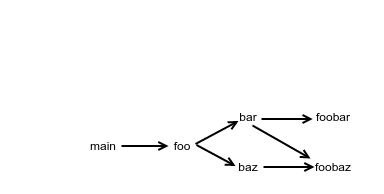
\includegraphics[width=3.5in, trim=0.8in 0in 0in 1.0in, clip]{callgraph.png}
%\caption{The call graph of the example program}
%\end{figure}
%
%I define a potential error revealing method (PERM) as the method that might trigger the dynamic condition of residual investigation for a FindBugs bug pattern.  For example, FindBugs reports an error when a class overrides the equals(Object) method but not the hashCode() method.  Residual investigation installs dynamic checks for the condition that Object.hashCode() is called on an object of a class that redefines equals(Object) and inherits the implementation of hashCode(). The method that contains a call to hashCode() on the suspect class (i.e. the class that redefines equals and inherits hashCode) or its subclass is the PERM for this bug pattern.  Another example is that FindBugs statically detects dropped exceptions and reports them.  Residual investigation examines which methods end up being dynamically invoked in the suspect code block and watches whether the same methods ever throw the dropped exception when called from anywhere in the program. The methods that contain calls to a method that can be invoked in the suspect code block and can throw exceptions are the PERMs for this bug pattern. I analyze the PERMs using text search such as grep and static analysis such as call graph analysis and Java reflection API.  For example, for the dropped exception pattern, I analyze the types of the exceptions declared to be thrown by the methods in the suspect code block (suspect methods) using Java reflection and then search for methods whose names are the same as that of any suspect method and throw the same exceptions using grep.  Suppose the method foobar in the above code example is our PERM.  
%
%Once finding a PERM, I interpose k levels back in the call graph from a PERM and call this a “switching” method.  Suppose k=1. In our example, the method bar is a switching method.  At the beginning I run existing system tests.  When I hit a switching method, I start exploring (i.e. switching to dynamic symbolic execution mode, instead of just dynamic execution).  To allow exploration, I relax (i.e., forget) some concrete values.  The first cut is to forget the arguments of switching methods.  In short, the invocation of a switching method turns on dynamic symbolic execution mode during the execution of an existing system test.  I declare victory when I find an approximate system test that calls the PERM method: the unit test case for bar that invokes foobar during its execution given the relaxed state.  In our example, this corresponds to a path like 
%
%\begin{figure}[h]
%\centering
%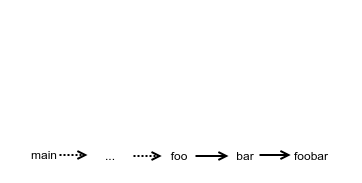
\includegraphics[width=3.5in, trim=0in 0in 0in 2.0in, clip]{path.png}
%\caption{The path that calls the PERM method in the example program}
%\end{figure}
%
%The dotted line arrow marks the path before I start dynamic symbolic exploration (i.e. the path exercised by the existing system test), while the solid line arrow marks the path that the generated unit test case for bar establishes. 
%
%PERM definitions for other bug patterns not mentioned in the above text:
%\begin{itemize}
%\item Bad Covariant Definition of Equals: FindBugs detects that programmers write equals method that accept a parameter of type other than Object.  Residual investigation checks whether the ancestral equals method, Object.equals(Object), is called on an instance of a class that has a covariant definition of equals.  The PERM for this bug pattern is the method that contains a call to equals() on the suspect class (i.e. the class redefines equals and inherits hashCode) or its subclass.
%\item Cloneable Not Implemented Correctly: This bug pattern does not require native test suite.  Thus, I do not need to improve existing test suite.
%\item Equals Method Overrides Equals in Super-class and May not Be Symmetric: FindBugs detects whether both the overriding equals method in the subclass and the overridden equals method in the superclass use instanceof in the determination of whether two objects are equal.  Residual investigation dynamically calls both equals method whenever it observes a comparison involving a contentious object and test if the results match.  The PERM for this bug pattern is the method that contains a call to equals() on the suspect superclass or subclass.
%\item Non-Short-Circuit Boolean Operator: FindBugs issues warnings for use of \sv{\&} and \sv{|} inside the condition of an if statement.  Residual investigation checks for actual side-effects on the right-hand side of a non-short-circuiting boolean operator.  The PERM for this bug pattern is the method that contains a \sv{\&} or \sv{|} in an if statement.
%\item Read Return Should be Checked: FindBugs checks if the return value from read in java.io.InputStream is ignored.  Residual investigation waits until it sees a read method on an object of any subclass of InputStream returns fewer bytes than requested (even for a call that does check the return value).  The PERM for this bug pattern is the method that contains a call to read on the suspect class.
%\end{itemize}



%\chapter{Management and Timeline}
%\label{chp:timeline}
%
%My overall goal is to defend the dissertation by September 2015.  I plan to submit a paper on the proposed work to ICSE 2016; the deadline for this conference is September 4, 2015.  Right now the underlying dynamic symbolic execution engine Dsc\cite{islam10dsc+mock} is similar to jCute\cite{sen06cute} released by University of Illinois at Urbana-Champaign. I plan to improve Dsc to make it become cutting-edge and open-sourced by the end of next March.  I plan to work out the required static analysis (e.g. call graph analysis) by May 2015.  I plan to finish the implementation of the proposed work by July 2015.  I will be writing the dissertation, performing implementations and evaluations, and plan to complete the dissertation by September 2015. 

\chapter{Residual Investigation: Predictive and Precise Bug Detection}
\label{chp:rfbipaper}
%\documentclass{acm_proc_article-sp}
%\documentclass[10pt,journal,letterpaper,compsoc]{IEEEtran}
%\documentclass[prodmode,acmtosem]{acmsmall} % Aptara syntax

%% % Package to generate and customize Algorithm as per ACM style
%% \usepackage[ruled]{algorithm2e}
%% \renewcommand{\algorithmcfname}{ALGORITHM}
%% \SetAlFnt{\small}
%% \SetAlCapFnt{\small}
%% \SetAlCapNameFnt{\small}
%% \SetAlCapHSkip{0pt}
%% \IncMargin{-\parindent}



%\title{Residual Investigation:\\Predictive and Precise Bug Detection}
%
%%% \author{Michael~Shell,~\IEEEmembership{Member,~IEEE,}
%%%         John~Doe,~\IEEEmembership{Fellow,~OSA,}
%%%         and~Jane~Doe,~\IEEEmembership{Life~Fellow,~IEEE}% <-this % stops a space
%\author{KAITUO LI
%\affil{University of Massachusetts, Amherst, USA}
%        CHRISTOPH REICHENBACH
%\affil{Goethe University Frankfurt, Germany}
%        CHRISTOPH CSALLNER
%\affil{University of Texas at Arlington, USA}
%        YANNIS SMARAGDAKIS
%\affil{University of Athens, Greece}
%}
% NOTE! Affiliations placed here should be for the institution where the
%       BULK of the research was done. If the author has gone to a new
%       institution, before publication, the (above) affiliation should NOT be changed.
%       The authors 'current' address may be given in the "Author's addresses:" block (below).
%       So for example, Mr. Abdelzaher, the bulk of the research was done at UIUC, and he is
%       currently affiliated with NASA.
% CR: According to this I should list myself as unaffiliated, but that
% seems silly.  I could change it to UMass, though.

%\begin{abstract}
%We introduce the concept of ``residual investigation'' for program
%analysis. A residual investigation is a dynamic check installed as a
%result of running a static analysis that reports a possible program
%error.  The purpose is to observe conditions that indicate whether the
%statically predicted program fault is likely to be realizable and
%relevant. The key feature of a residual investigation is that it has
%to be much more precise (i.e., with fewer false warnings) than the
%static analysis alone, yet significantly more general (i.e., reporting
%more errors) than the dynamic tests in the program's test suite that
%are pertinent to the statically reported error. That is, good residual
%investigations encode dynamic conditions that, when considered in
%conjunction with the static error report, increase confidence in the
%existence or severity of an error without needing to
%directly observe a fault resulting from the error.
%
%We enhance the static analyzer FindBugs with several residual
%investigations, appropriately tuned to the static error patterns in
%FindBugs, and apply it to 9 large open-source systems and their native
%test suites. The result is an analysis with a low occurrence of false
%warnings (``false positives'') while reporting several actual errors
%that would not have been detected by mere execution of a program's
%test suite. 
%\end{abstract}

%\category{D.2.5}{Software Engineering}{Testing and Debugging -- debugging aids}
%\category{B.8.1}{Performance and Reliability}{Reliability, Testing, and Fault-Tolerance}
%
%\terms{Design, Reliability, Verification}
%% \keywords{Static analysis, bugs, false warnings, FindBugs, RFBI, software testing, existing test cases, dynamic analysis}
%\keywords{False warnings, existing test cases, RFBI}
%
%
%\acmformat{Kaituo Li, Christoph Reichenbach, Christoph Csallner, and
%Yannis Smaragdakis, 2013.
%Residual Investigation: Predictive and Precise Bug Detection.
%}
% At a minimum you need to supply the author names, year and a title.
% IMPORTANT:
% Full first names whenever they are known, surname last, followed by a period.
% In the case of two authors, 'and' is placed between them.
% In the case of three or more authors, the serial comma is used, that is, all author names
% except the last one but including the penultimate author's name are followed by a comma,
% and then 'and' is placed before the final author's name.
% If only first and middle initials are known, then each initial
% is followed by a period and they are separated by a space.
% The remaining information (journal title, volume, article number, date, etc.) is 'auto-generated'.

%\begin{bottomstuff}
%Authors' addresses: K. Li, Computer Science Department,
%University of Massachusetts, Amherst, MA 01003, USA;
%C. Reichenbach, Department of Informatics and Mathematics,
%Goethe-University Frankfurt, 60054 Frankfurt am Main, Germany;
%C. Csallner, Department of Computer Science and Engineering,
%University of Texas at Arlington, Arlington, TX 76019, USA;
%Y. Smaragdakis, Department of Informatics,
%University of Athens, Athens 15784, Greece.
%
%This is a revised and extended version of \cite{rfbi-issta12}
%which was presented at ISSTA~2012 and received an ACM SIGSOFT
%Distinguished Paper Award.
%\end{bottomstuff}

%\maketitle

A tension exists between static analysis and testing.  Static analysis has the problem of issuing false positives: namely, it often warns about bugs that are not real bugs.  They are just there because of over-generalizing observations.  However, testing suffers from no false positives.  When it reports an error, it's a true error.  In converse, testing suffers from false negatives: it misses many errors.  It only watches errors that are dynamically exercised by the test suite, whereas static analysis generalizes the test suite, or generalizes what the application would normally do.  Static analysis does not even need a test suite.  Therefore static analysis has fewer false negatives.  That's a traditional tension between static analysis and testing.  Ideally, what we would like is to have something in the middle.  And what can come in the middle is what we usually call dynamic analysis. But it is not well defined by what we mean by dynamic analysis.  We believe that ideally dynamic analysis are things that sit in the middle and get the best of both worlds, both static analysis and testing.  

This chapter investigates predictive and precise dynamic analysis.  The thrust of this  dynamic analysis is to have very few false positives and fewer negatives than testing.  Predictive and precise dynamic analysis can be combined with static analysis to improve precision and recall of bug detection. We have confirmed the efficacy of this combination  by implementing it inside FindBugs, a static bug detection tool. 

\section{Introduction and Motivation}
\label{introduction}

False error reports are the bane of automatic bug detection---this
experience is perhaps the most often-reported in the program analysis
research literature
\cite{musuvathi03lessons,zitser04testing,wagner05comparing,rutar04comparison,Ayewah:2010:GFF:1831708.1831738}.
Programmers are quickly frustrated and much less likely to trust an
automatic tool if they observe that reported errors are often not real
errors, or are largely irrelevant in the given context. This is in
contrast to error detection at early stages of program development,
where guarantees of detecting all errors of a certain class (e.g.,
type soundness guarantees) are desirable. Programmers typically
welcome conservative sanity checking while the code is actively being
developed, but prefer later warnings (which have a high cost of
investigation) to be issued only when there is high confidence that
the error is real, even at the expense of possibly missing errors.

The need to reduce false or low-value warnings raises difficulties
especially for static tools, which, by nature,
overapproximate program behavior. This has led researchers to devise
combinations of static analyses and dynamic observation of faults
(e.g., \cite{csallner05check,csallner06dsd-crasher,godefroid05dart,cadar05execution,tomb07variably,tillmann08pex,Islam14Generating})
in order to achieve higher certainty than purely static approaches.

In this article we identify and present a new kind of combination of
static and dynamic analyses that we term \emph{residual investigation}.
A residual investigation is a dynamic analysis that serves as the
run-time agent of a static analysis. Its purpose is to determine with higher
certainty whether the error identified by the static analysis is
likely true. In other words, one can see the dynamic analysis as the
``residual'' of the static analysis at a subsequent stage: that of
program execution. The distinguishing feature of a residual investigation,
compared to past static-dynamic combinations, is that the residual
investigation does not intend to report the error only if it actually
occurs, but to identify \emph{general} conditions that reinforce the
statically detected error. That is, a residual investigation is a
\emph{predictive} dynamic analysis, predicting errors in executions
not actually observed.  The predictive nature of residual investigation
is a significant advantage in practice: high-covering test inputs are hard to produce for
complex programs. 
% Given limited test inputs, residual investigation 
%can still detect a lot of bugs. This makes residual investigation more 
%feasible in practice compared to past static-dynamic combinations.

Consider as an example the ``equal objects must have equal hashcodes''
analysis (codenamed HE) in the FindBugs static error detector for Java
\cite{hovemeyer04finding,hovemeyer07finding,Ayewah:2010:GFF:1831708.1831738}. The HE
analysis emits a warning whenever a class overrides the method
\sv{equals(Object)} (originally defined in the \sv{Object} class, the
ancestor of all Java classes) without overriding the \sv{hashCode()}
method (or vice versa). The idea of the analysis is that the hash code
value of an object should serve as an equality signature, so a class
should not give a new meaning to equality without updating the meaning
of \sv{hashCode()}. An actual fault may occur if, e.g., two objects
with distinct hash code values are equal as far as the \sv{equals}
method is concerned, and are used in the same hash table. 
%This error
%will be hard to trace, as it can lead to a violation of fundamental
%program invariants. 
The programmer may validly object to the error
warning, however: objects of this particular class may never be used
in hash tables in the current program.  Our residual investigation
consists of determining whether (during the execution of the usual
test suite of the program) objects of the suspect class are ever
used inside a hash table data structure, or otherwise have their
\sv{hashCode} method ever invoked. (The former is a strong indication
of an error, the latter a slightly weaker one.)  Note that this will
likely not cause a failure of the current test execution: all objects
inserted in the hash table may have distinct hash code values, or
object identity in the hash table may not matter for the end-to-end
program correctness. Yet, the fact that objects of a suspect type
are used in a suspicious way is a very strong indication that the
program will likely exhibit a fault for different inputs. In this way
the residual investigation is a predictive dynamic analysis: it is
both more general than mere testing and more precise than static analysis.

We have designed and implemented residual investigations for several
of the static analyses/bug patterns in the FindBugs system. The result
is a practical static-dynamic analysis prototype tool, RFBI (for
\emph{Residual FindBugs Investigator}). Our implementation uses
standard techniques for dynamic introspection and code interposition,
such as bytecode rewriting and customized AspectJ aspects
\cite{aspectj}. The addition of extra analyses is typically hindered
only by engineering (i.e., implementation) overheads. Designing
the residual investigation to complement a specific static pattern
requires some thought, but it is typically quite feasible, by
following the residual investigation guidelines outlined earlier: the
analysis should be significantly more general than mere testing while
also offering a strong indication that the statically predicted fault
may indeed occur.

We believe that the ability to easily define such analyses is
testament to the value of the concept of residual investigation.
Predictive dynamic analyses are usually hard to invent. To our
knowledge, there are only a small number of predictive dynamic analyses
that have appeared in the research literature. (A standard example of
a predictive dynamic analysis is the Eraser race detection algorithm
\cite{266641}: its analysis predicts races based on inconsistent
locking, even when no races have appeared in the observed execution.)
In contrast, we defined several predictive analyses in a brief
period of time,
by merely examining the FindBugs list of bug patterns under the lens
of residual investigation. 

%The present article revises, generalizes, and extends the original
%conference publication on residual investigation \cite{rfbi-issta12}.
%Thus, we integrate the original definition and presentation of
%residual investigation analyses in RFBI, but our presentation also
%reflects a broader perspective on how residual investigation can apply
%to different contexts, the enabling factors and limitations
%of the approach, and more.

In summary, the main contributions of this work are:
\begin{itemize}
\item We introduce residual investigation as a general concept and
illustrate its principles.
\item We implement residual investigations for several of the most
common analyses in the FindBugs system, such as ``cloneable not
implemented correctly'', ``dropped exception'', ``read return should
be checked'', and several more. This yields a concrete result of our
work, in the form of the Residual FindBugs Investigator (RFBI)
tool.
\item We validate our expectation that the resulting analyses are useful by
applying them to 9 open-source applications (including large systems,
such as JBoss, Tomcat, NetBeans, and more) using their native
test suites. We find that residual investigation produces numerous
(31) warnings that do not correspond to test suite failures and
are overwhelmingly bugs.
\item We discuss the applicability of residual investigation to
several other static analyses in the literature. These include
race detection, SQL injection analyses, and other pattern-based
code analyses in FindBugs. We also discuss how the quality of
the test suite affects the applicability of residual investigation.
\end{itemize}

%The rest of the article is organized as follows. We begin with a
%description of our approach to residual investigation and the kinds of
%analyses we have defined (Section~\ref{our-analyses}).  \cite{fixit}


%\begin{figure}[tbp]
%\begin{verbatim}
%int testme(int x, int y) {
%  int prod = x*y;
%  if (prod < 0)
%    throw new ArgumentException();
%  if (x < y) {     // swap them
%    int tmp = x;
%    x = y;
%    y = tmp;
%  }
%  int sqry = y*y;
%  return prod*prod - sqry*sqry;
%}
%\end{verbatim}
%\caption{An example method whose invariants we want to infer.}
%\label{ex1}
%\end{figure}


\section{Residual Investigation}
\label{our-analyses}

Residual investigation is a simple concept---it is a vehicle that
facilitates communication rather than a technical construction with a
strict definition. We next discuss its features and present
the example analyses we have defined.

\subsection{Background and General Concept}

We consider a dynamic check that is tied to a
static analysis to be a residual investigation if it satisfies the informal
conditions outlined in Section~\ref{introduction}:
\begin{itemize}
\item The check has to identify with very high confidence that the
statically predicted behavior (typically a fault\footnote{The
computing literature is remarkably inconsistent in the use of the
terms ``error'', ``fault'', ``failure'', etc. In plain English
``error'' and ``fault'' are dictionary synonyms. Mainstream Software
Engineering books offer contradicting definitions (some treat an
``error'' as the cause and a ``fault'' as the observed symptom, most
do the opposite). Standard systems parlance refers indiscriminately to
``bus errors'' and ``segmentation faults'', both of which are quite
similar program failures. In this article we try to consistently treat
``error'' (as well as ``bug'' and ``defect'') as the cause (in the
program text) of unexpected state deviation, and ``fault'' as the
dynamic occurrence that exhibits the consequences of an error. That is
we think of \emph{programming} errors, and \emph{execution} faults. It
should also be possible for the reader to treat the two terms as
synonyms.}) is valid and relevant for actual program executions. A
residual investigation should substantially reduce the number of false (or
low-value) error reports of the static analysis.
\item The analysis has to be predictive: it should be generalizing
significantly over the observed execution. A residual investigation should
recognize highly suspicious behaviors, not just executions with faults. 
This is a key requirement, since it is easier to have a test case 
to expose suspicious behaviors than to have a test case to actually cause
 faults.
\end{itemize}


A bit more systematically, we can define the following predicates
over a program $p$:
\begin{itemize}
\item $B_p(b)$, for ``$p$ has bug $b$'', i.e., the program text contains an
   error, $b$, of a kind we are concerned with (e.g., class
   overrides \sv{equals} but not \sv{hashcode}) and there is some
   execution $e_p$ of $p$ for which this error leads to a fault.
\item $S_p(b)$, for ``$p$ induces a static error report on bug $b$'', i.e., the program
   text contains a possible error that the static analysis reports.
\item $T_p(b)$, for ``$p$ causes a test case fault due to bug $b$'', when executed with $p$'s  
   test suite.
\item $R_p(b)$, for ``$p$ triggers the residual investigation
  (dynamic) check'' (associated with the static report for bug $b$),
  when executed with $p$'s test suite.
\end{itemize}

% \CC{The definitions in Section 2.1 still do not make sense to me:
% - What does p in Figure 1 represent? It seems to represent all
%		bugs that are theoretically possible in a given program p.
% - The definition of S_p(b) ("p induces a static error report on bug b")
%		is confusing as it sounds like b "is a bug". But S does not
%		imply B.
% - The definition of R_p(b) is also confusing, see S_p(b).}


% \CC{Notes towards a systematic technique for deriving dynamic checks:
% (1) Programmer objections can be of two kinds:
%	(a) The static analysis is not sound---it does not fully 
%	understand the semantics of the programming language 
%	(inter-procedural reasoning, reflection, native code, loops, and 
%	other tricky language constructs).
%	(b) The static analysis does not fully understand the conventions
%	we are using in this particular program (``We never use instances
%	of this class in a hashed data structure'', etc.)
% (2) Dynamic checks can check for (1a) or (1b) or both.
% (3) You want the dynamic checks to be predictive..}

Although we typically use the term ``residual investigation'' for
the dynamic analysis, the error reporting process includes the static
analysis. That is, a residual investigation issues a reinforced warning
in case the static analysis predicted an error and the dynamic analysis
confirms it, i.e., in case $S_p(b) \wedge R_p(b)$.

We assume that 
% our static analysis is complete for the kinds of errors
% we consider, and 
the dynamic testing is sound for the execution it
examines.\footnote{
% This assumption holds only for the purposes of the 
% formalism in this sub-section. The notion of residual investigation holds perfectly well 
% for incomplete bug finders.  
We view all analyses as bug detectors, not as
correctness provers. Therefore soundness means that warning about an
error implies it is a true error, and completeness means that having
an error implies it will be reported. For a correctness prover the two
notions would be exactly inverse.} Thus, we have:
% \[ \forall p: B_p(b) \Rightarrow S_p(b) \] (by completeness of static analysis)
\[ \forall p, b: T_p(b) \Rightarrow B_p(b) \] 
% (by soundness of dynamic testing).

\begin{figure}
\centering
% 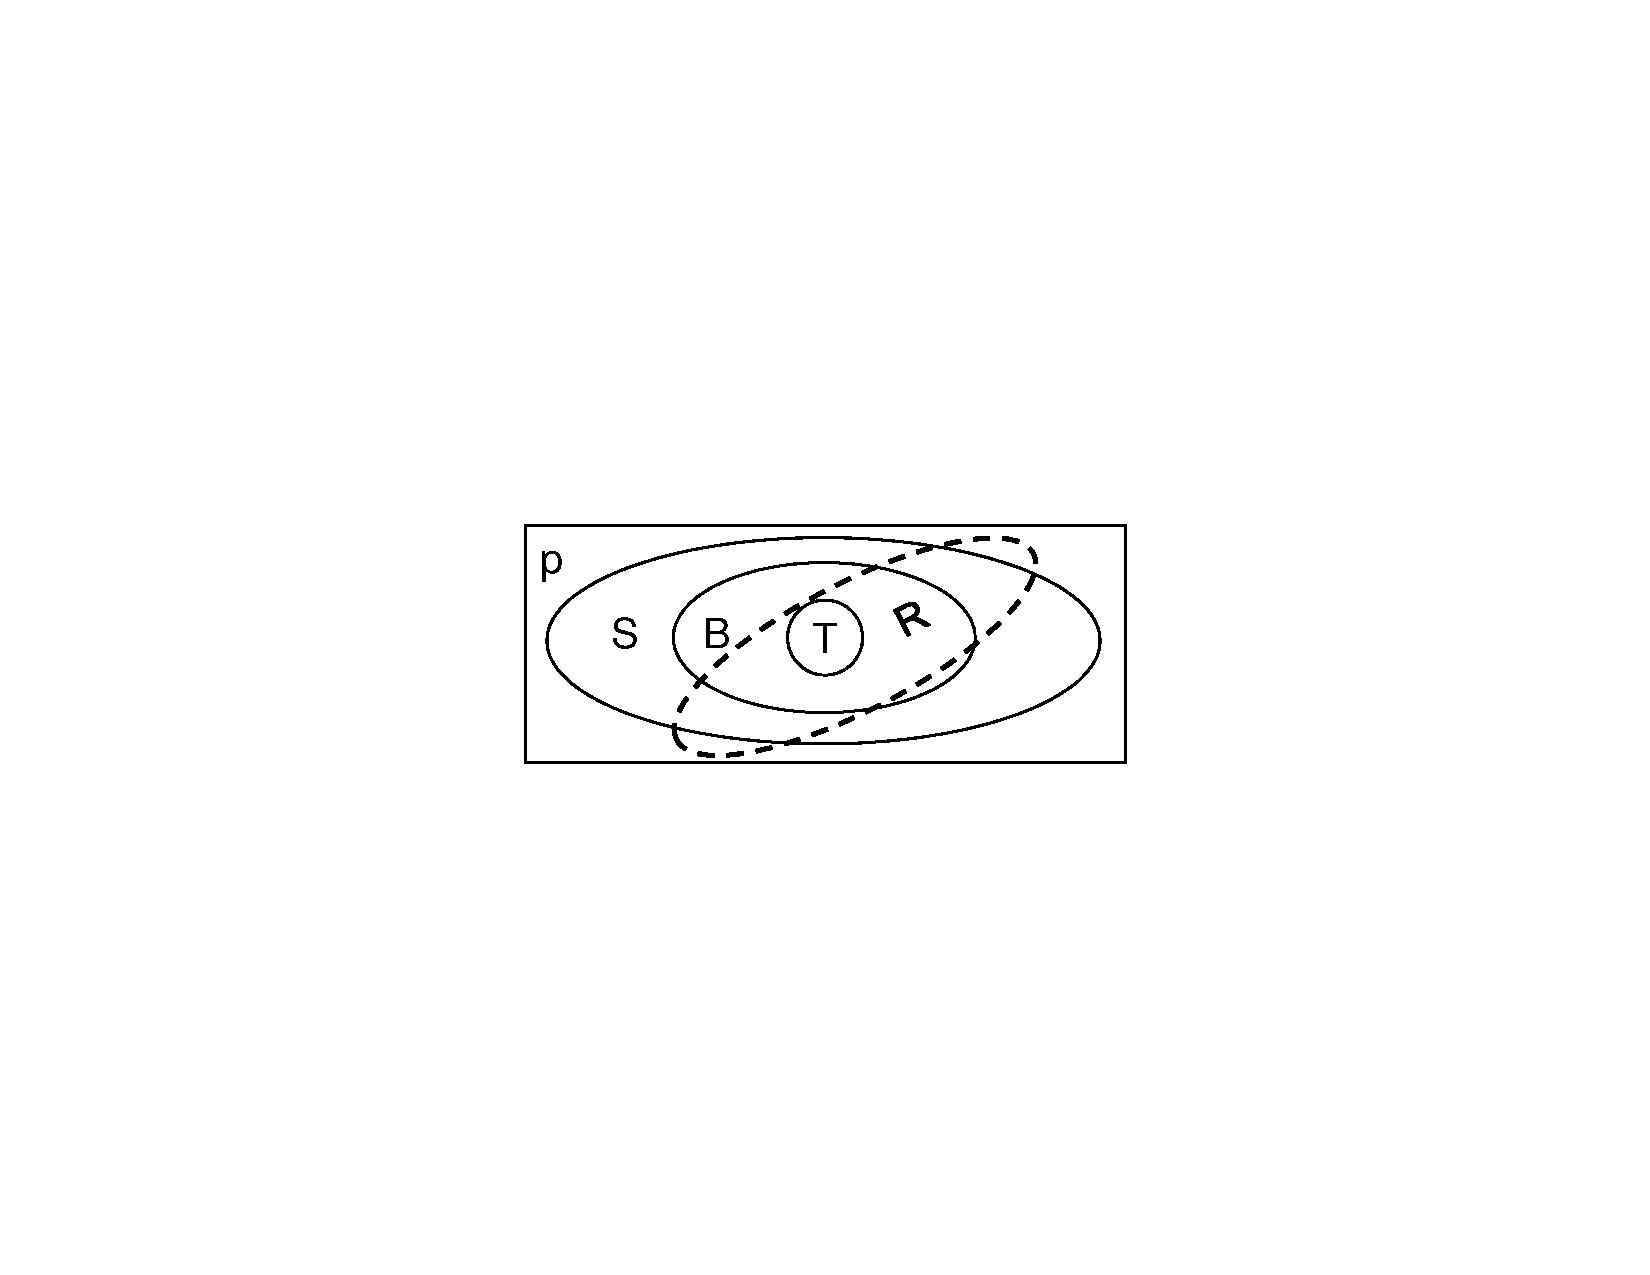
\includegraphics[width=2in, trim=3.25in 3.25in 3.25in 3.25in, clip]{prelim.pdf}
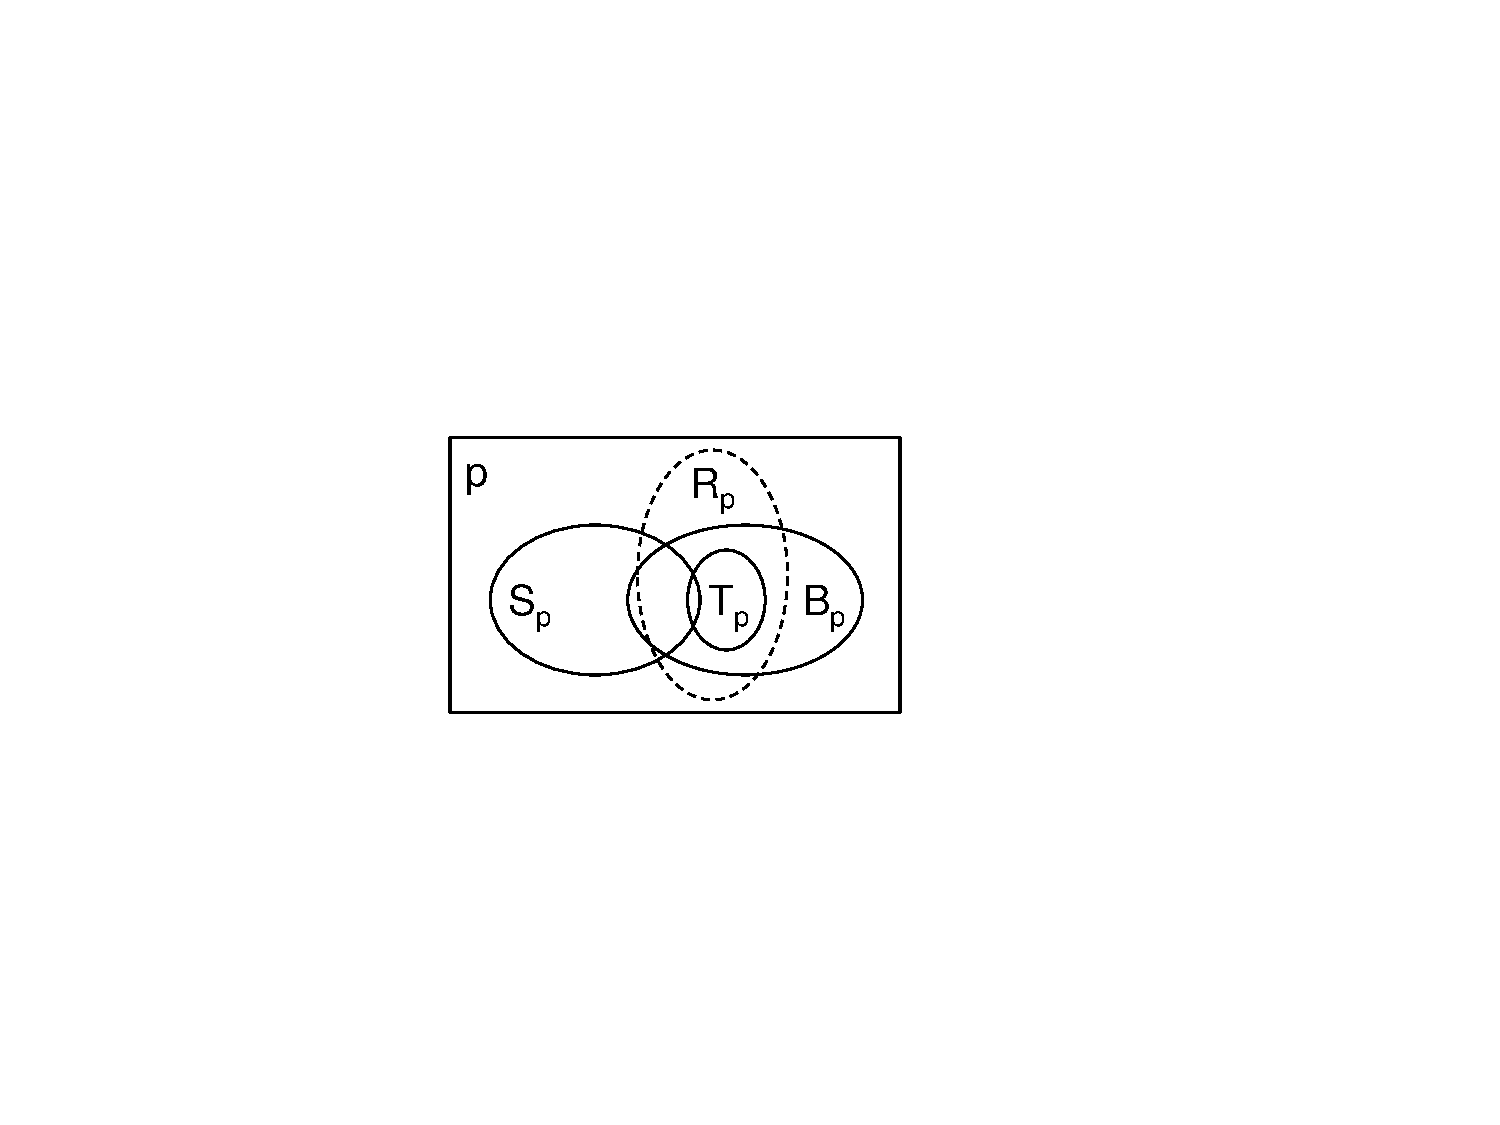
\includegraphics[width=1.5in, trim=2.9in 2.7in 3.9in 2.8in, clip]{prelim_S-incomplete.pdf}
\caption{The goal of residual investigation ($R_p$) of a program $p$ is to provide a filter for 
the static bug warnings ($S_p$), such that $R_p$ and $S_p$ combined 
(i.e., the intersection of $R_p$ and $S_p$) better approximates 
the program's set of true bugs ($B_p$) than static analysis alone.}
% and dynamic testing (T).}
% \CC{It is hard to compare R with T. They are different, but it is not
% clear which one approximates B better. R seems to be cheaper though, as
% you do not have to manually write any test cases.}
\label{fig:prelim}
\end{figure}

The requirements for having a valid and useful residual investigation then
become:
\begin{enumerate}

% \item A residual investigation should be complete with respect to the 
% dynamic testing, hence:
% \[ \forall p: T_p(b) \Rightarrow R_p(b) \]

%% [YANNIS]: I agree. But it's a matter of definitions. One can always
%% take R to be T || R_original. E.g., we can consider any test suite
%% failure to be a residual investigation failure. No matter, this is
%% a non-essential point, so it's better removed.
%% question by CC: Why do we want (T ==> R) to hold?
%% As the programmer runs R on the test suite T anyways, she already
%% has T to find the bugs that T can find. There is no need for R
%% to replicate these bug warnings. I think we can relax that
%% requirement without losing anything.
%% Also, it seems that (T ==> R) does not hold for some of the
%% detectors such as "Non-Short-Circuit Boolean Operator (NS)".

\item The static analysis is unsound (i.e., some warnings are
false):
\[ \exists p,b: S_p(b) \wedge \neg B_p(b) \]
% (We are only interested in non-trivial and therefore undecidable 
% program properties. As our static analysis is complete, it has to be
% unsound.
(As discussed in the introduction, this assumption is true for most
static analysis systems, as they produce false warnings.%
%% Note that since $T$ is sound, this implies $\exists p,b: S_p(b) \wedge
%% \neg T_p(b)$ i.e., the dynamic analysis also does not flag this program
%% that the static analysis flags.
%% CR: What it really says is that there are bugs that are reported by
%% static checkers but not flagged by unit tests.  While that's true,
%% I don't see how it adds to the discussion at this point.
)

\item The dynamic testing (of a program's test suite) is
incomplete (i.e., bugs are missed by testing):
\[ \exists p,b: B_p(b) \wedge \neg T_p(b) \]
(Again, the undecidability of non-trivial program properties combined
with the soundness of testing implies testing is incomplete.)

\item The residual investigation should be an appropriate bridge for
the gap between the static analysis and the bug (see also
Figure~\ref{fig:prelim}):
\[ \forall p, b: B_p(b) \textrm{\ approximately iff\ } S_p(b) \wedge  R_p(b) \]
%% CR: let's not mix predicate and set notation.  Yes, 90% of our
%% readers understand this, but the only reason I can see for
%% switching notation styles here is that there's no tilde-\iff.  But
%% since we're informal anyway, that does not seem like a good excuse.
This is the only
informal notion in the above. It is practically impossible to have
exact equivalence for realistic programs and error conditions, since
$R_p(b)$ examines a finite number of program executions. Note that
(approximate) equivalence means both that $S_p(b) \wedge R_p(b)$ (likely)
implies a bug $b$ exists
% (i.e., $S_p(b) \wedge R_p(b) \Rightarrow B_p(b)$)
and that, if there is a bug $b$, $S_p(b) \wedge R_p(b)$ will (likely) be true. 
% (i.e., $B_p(b) \Rightarrow R_p(b)$).
In practice, we place a much greater weight on the former direction of
the implication. That is, we are happy to give up on completeness
(which is largely unattainable anyway) to achieve (near-)soundness of
error warnings. 
%%% YS: I am not sure what this adds.
% For instance, residual investigation does not consider the bugs
% missed by static analyses due to reflection. No static analyses%
% that we know of over-approximate in the presence of reflection.
% They all accept incompleteness and move on. We only consider t%he
% bugs that can be issued by static analysis tools and try to reduce
% false positives among them.
\end{enumerate}

The question then becomes: how does one identify a good residual
investigation? We have used some standard steps:
\begin{itemize}
\item Start with the static analysis and identify under what
conditions it is \emph{inaccurate} (produces false positives) or \emph{irrelevant} (produces true but low-value positives).
\item Estimate how likely these conditions can be. In other words, is
this static analysis likely to yield error reports that the programmer
will object to, seeing them as false or of low-value?
\item If so, is there a concise set of dynamic information (other than
a simple fault) that can invalidate the programmer's objections? That is,
can we determine based on observable dynamic data if the likely
concerns of a programmer to the static warnings do not apply?
\end{itemize}

Recognizing such ``likely objections of the programmer'' has been the
key part in our design. With this approach we proceeded to identify
residual investigations for seven static analyses in the FindBugs
system, including some of the analyses that issue the most common
FindBugs warnings.


%\CC{The new definition of R is better. But the word ``residual''
%still implies that R is a subset of S, as a residual analysis will
%only inspect S-warnings. But in this section we use R in the sense
%of ``dynamic check installed blindly on all classes, without running
%any static analysis to guide the installation''.}
%\YS{I don't agree. We don't use R as a check installed in all classes.
%It is only installed in classes that need it. But it also does not
%watch for all conditions that enable the static analysis. I.e., it
%is not a subset. If I'm looking for a dropped exception at one point
%in the program (detected statically) and I check for that exception 
%at all sites calling
%the same method, then I'm not a subset of the static scenario yet
%directly influenced by it.}
% \CC{RFBI only installs dynamic checks to investigate warnings produced
% by the static analysis. So RFBI will never produce a warning about
% something the static analysis has not warned about. But in Section 2.1
% we use R_p(b) as if the dynamic check is installed regardless of what
% the static analysis says. Then we say that RFBI intersects S_p(b) with
% R_p(b).}

%\YS{I am not sure we should burden this section with that. Also,
%  I don't understand the point about T. RFBI does not trigger T.}
%
%\CC{Maybe we should make the following assumption explicit. We assume 
%that the existing test suite mainly (only) contains ``happy paths'',
%i.e., paths that reflect real-world program execution scenarios. On the
%other hand, if the test suite would only check that the application 
%rejects input values that can never occur in practice, then RFBI warnings
%would not be very interesting.}
%
%\CC{Based on ``T only contains happy paths'', we could also say 
%explicitly that RFBI follows the executions of the test suite
%precisely. That is, RFBI wants to get credibility from the existing
%test suite. We say ``look, it can happen in a real execution''. So
%we are not interested in tweaking the existing test suite. Hence
%running the resdiual analysis will trigger $T_p(b)$. As we said before,
%it is a matter of definition, as R does not really have to contain T.
%There is no need for RFBI to reproduce T, as RFBI triggers T anyways.}
%


\subsection{Catalog of Analyses}

We next present the residual investigations defined in our RFBI
(Residual FindBugs Investigator) tool, each tuned to a static analysis
in the FindBugs system.
We list each analysis (uniquely described by the corresponding
FindBugs identifier) together with the likely user \emph{objections}
we identified and a description of \emph{clues} that dynamic analysis
can give us to counter such objections.  To simplify the presentation,
we detail our implementation at the same time.
%%  We separate the definition of each analysis
%% from the way it is implemented, but choose to present them grouped
%% together, to avoid the need to revisit each analysis definition to
%% describe its implementation.

%Just
%like other dynamic analyses, implementing residual investigations
%can be complex. 


\subsubsection{Bad Covariant Definition of Equals (Eq)}

The \sv{equals(Object)} method is defined in the \sv{Object} class
(\sv{java.lang.Object}) and can be overridden by any
Java class to supply a user-defined version of object value
equality. A common mistake is that programmers write \sv{equals}
methods that accept a parameter of type other than \sv{Object}. The
typical case is that of a covariant re-definition of \sv{equals},
where the parameter is a subtype of \sv{Object}, as in the example
class \sv{Pixel}:

\begin{small}
\begin{verbatim}
class Pixel { 
  int x; 
  int y; 
  int intensity; 

  boolean equals(Pixel p2) 
  { return x==p2.x && y==p2.y; }
} 
\end{verbatim}
\end{small}

This \sv{equals} method does not override the \sv{equals} method in
\sv{Object} but instead overloads it for arguments of the appropriate,
more specific, static type. As a result, unexpected behavior will
occur at runtime, especially when an object of the class type is
entered in a Collections-based data structure (e.g., \sv{Set},
\sv{List}). For example, if one of the instances of \sv{Pixel} is put
into an instance of a class implementing interface \sv{Container}, then
when the \sv{equals} method is needed, \sv{Object.equals()} will get
invoked at runtime, not the version defined in \sv{Pixel}. One of the
common instances of this scenario involves invoking the
\sv{Container.contains(Object)} method. A common skeleton for
\sv{Container.contains(Object)} is:

\begin{small}
\begin{verbatim}
boolean contains(Object newObj) {
  for (Object obj : this) {
    if (obj.equals(newObj))
      return true;
  }
  return false;
}
\end{verbatim}
\end{small}

Here, \sv{contains(Object)} will use
\sv{Object.equals}, which does not perform an appropriate
comparison: it compares references, not values. Therefore, objects of
type \sv{Pixel} are not compared in the way that was likely intended.

\objection 
FindBugs issues an error report for each occurrence of a covariant
definition of \sv{equals}. Although the covariant definition of
\sv{equals} is very likely an error, it is also possible that no error
will ever arise in the program. This may be an accidental artifact of
the program structure, or even a result of the programmer's
calculation that for objects of the suspect class the dynamic type
will always be equal to the static type, for every invocation of
\sv{equals}. For instance, the redefined \sv{equals(Pixel)} method may
be used only inside class \sv{Pixel}, with arguments that are always
instances of subtypes of \sv{Pixel}, and the programmer may have
chosen the covariant definition because it is more appropriate and
convenient (e.g., obviates the need for casts). 

%% [YANNIS]: Again, it's a matter of definitions, not substance.
%% Abstractly, R can be viewed as the dynamic part, although the
%% implementation really checks R && S.
%% question by CC: In the preliminary discussion, we separated S and R.
%% I.e., we said that R is a filter for S, such that (S && R) == B. 
%% In this concrete detector description, we present the detector as 
%% the combination of S and R.
%% I.e., the core of this detector is really just 
%% "record calls to Object.equals(Object)".
%% If we stick with the current combined presentation of S and R
%% then I wonder, why we did not say "S == B".

\clue Our residual investigation consists of simply checking whether
the ancestral \sv{equals} method, \sv{Object.equals(Object)}, is
called on an instance of a class that has a covariant definition of
\sv{equals}. The implementation first enters suspect classes into a
blacklist and then instruments all call sites of
\sv{Object.equals(Object)} to check whether the dynamic type of the
receiver object is in the blacklist.

\implementation 
We transform the
application bytecode, using the ASM Java bytecode engineering library.
Generally, for all our analyses, we instrument
incrementally (i.e., when classes are loaded), except in
applications that perform their own bytecode rewriting which may
conflict with load-time instrumentation. In the latter case, we
pre-instrument the entire code base in advance (build time).


\subsubsection{Cloneable Not Implemented Correctly (CN)}

%% comment by CC: Cloneable is hard to understand. It is completely
%% broken in Java, to the point people may consider it irrelevant. 
%% Quoting Joshua Bloch from Effective Java [2nd edition, page 61]:
%% "Because of its many shortcomings, some expert programmers simply
%% choose never to override the clone method and never to invoke it [..]"
%% I would move this subsection further to the back, as it may 
%% otherwise confuse and turn off people early on.

Java is a language without direct memory access, hence generic object
copying is done only via the convention of supplying a \sv{clone()}
method and implementing the \sv{Cloneable} interface. Additionally,
the \sv{clone()} method has to return an object of the right dynamic
type: the dynamic type of the returned object should be the same as
the dynamic type of the receiver of the \sv{clone} method and
\emph{not} the (super)class in which the executed method \sv{clone}
happened to be defined. This is supported via a user convention: any
definition of \sv{clone()} in a class \sv{S} has to call
\sv{super.clone()} (i.e., the corresponding method in \sv{S}'s
superclass). The end result is that the (special) \sv{clone()} method
in the \sv{java.lang.Object} class is called, which always produces an object
of the right dynamic type.

\objection
FindBugs statically detects violations of the above convention and reports
an error whenever a class implements the \sv{Cloneable} interface, but
does not directly invoke \sv{super.clone()} in its \sv{clone} method
(typically because it merely creates a new object by calling a
constructor). Although this condition may at first appear to be quite
accurate, in practice it often results in false error reports because
the static analysis is not inter-procedural. The \sv{clone} method may
actually call \sv{super.clone()} by means of invoking a different
intermediate method that calls \sv{super.clone()} and returns the
resulting object.

\clue
A dynamic check that determines whether a \sv{clone} method definition
is correct consists of calling \sv{clone} on a subclass of the
suspect class \sv{S} and checking the return type (e.g., by casting
and possibly receiving a \sv{ClassCastException}).  Our residual
investigation introduces a fresh subclass \sv{C} of \sv{S} defined and used
(in a minimal test case) via the general pattern:

\begin{small}
\begin{verbatim}
class C extends S { 
  public Object clone() 
  { return (C) super.clone(); }
} 
... ((new C()).clone()) // Exception 
\end{verbatim}
\end{small}

\noindent If \sv{S} does not have a no-argument constructor, we statically
replicate in \sv{C} all constructors with arguments and dynamically
propagate the actual values of arguments used for construction of
\sv{S} objects, as observed at runtime.

If the test case results in a \sv{ClassCastException} then the
definition of \sv{clone} in class \sv{S} is indeed violating
convention. Conversely, if \sv{S} implements the \sv{clone} convention
correctly (i.e., indirectly calls \sv{super.clone()}) no exception is
thrown. This test code is executed the first time an object of class
\sv{S} is instantiated. In this way, if class \sv{S} does not get used
at all in the current test suite, no error is reported.

The above residual investigation provides a very strong indication of
a problem that will appear in an actual execution of the program,
without needing to observe the problem itself. Indeed, the current
version of the program may not even have any subclasses of \sv{S}, but
a serious error is lurking for future extensions.

\implementation 
Our implementation of this analysis uses AspectJ to introduce the
extra class and code. In the case of complex constructors, we retrieve
those with Java reflection and use AspectJ's constructor joinpoints
instead of generating customized calls. A subtle point is that if the
superclass, \sv{S}, is declared \sv{final} or only has private constructors, the residual
investigation does not apply. This is appropriate, since the absence
of any externally visible constructor suggests this class is not to be
subclassed. Similarly, the generated code needs to be in the same
package as the original class \sv{S}, in order to be able to access
package-protected constructors.


\subsubsection{Dropped Exception (DE)}

Java has \emph{checked exceptions}: any exception that may be thrown
by a method needs to either be caught or declared to be thrown in the
method's signature, so that the same obligation is transferred to
method callers. To circumvent this static check, programmers may catch
an exception and ``drop it on the floor'', i.e., leave empty the
\sv{catch} part in a \sv{try}-\sv{catch} block. FindBugs statically
detects dropped exceptions and reports them.

\objection
Detecting all dropped exceptions may be a good practice, but is also
likely to frustrate the programmer or to be considered a low-priority
error report. After all, the type system has already performed a check
for exceptions and the programmer has explicitly disabled that check
by dropping the exception. The programmer may be legitimately certain
that the exception will never be thrown in the given setting (a common
case---especially for I/O classes---is that of a general method that
may indeed throw an exception being overridden by an implementation
that never does).

\clue
Our residual investigation consists of examining which methods end up
being dynamically invoked in the suspect code block and watching
whether the same methods ever throw the dropped exception when called
from \emph{anywhere} in the program. For instance, the following code
snippet shows a method \sv{meth1} whose \sv{catch} block is empty. In
the \sv{try} block of \sv{meth1}, first \sv{foo1} is executed, then
\sv{foo2} (possibly called from \sv{foo1}), then \sv{foo3}, and so on:

\begin{small}
\begin{verbatim}
void meth1() { 
  try { 
    foo1(); 
    //Call-graph foo1()->foo2()->...->fooN() 
  } catch(XException e) { }  //empty 
}
\end{verbatim}
\end{small}

%\vspace{-2mm}

The residual investigation will report an error if there is any other
method, \sv{methX}, calling some \sv{foo$i$} where \sv{foo$i$} throws an
\sv{XException} during that invocation (regardless of whether that
exception is handled or not):

\begin{small}
\begin{verbatim}
void methX {  
  try { ...
    //Call-graph ...->fooN()->... 
  } catch(XException e) { 
    ...  // handled
  } 
} 
\end{verbatim}
\end{small}

In this case the user should be made aware of the possible threat.  If
\sv{foo$i$} can indeed throw an exception, it is likely to throw it in
any calling context. By locating the offending instance, we prove to
programmers that the exception can occur.  Although the warning may
still be invalid, this is a much less likely case than in the purely
static analysis.

\implementation 
The implementation of this residual investigation uses
both the ASM library for bytecode transformation and AspectJ, for ease
of manipulation.

We execute the program's test suite twice. During the first pass, we
instrument the beginning and end of each empty \sv{try}-\sv{catch} block
with ASM, then apply an AspectJ aspect to
find all methods executed in the dynamic scope of the
\sv{try}-\sv{catch} block (i.e., transitively called in the block)
that may throw the exception being caught.\footnote{To apply the
combination of ASM and AspectJ at load time, we had to make two
one-line changes to the source code of AspectJ. The first allows
aspects to apply to ASM-transformed code, while the second allows
AspectJ-instrumented code to be re-transformed.} (We also check
that there is no intermediate method that handles the  exception,
by analyzing the signatures of parent methods on the call stack.)
In the first pass we collect all such methods and generate
custom AspectJ aspects for the second pass.  During the second pass,
we then track the execution of all methods we identified in the first pass
and identify thrown exceptions of the right type. For any such exception
we issue an RFBI error report.

%all thrown exceptions are observed, using AspectJ instrumentation.  For
%each thrown exception, we register its dynamic type and the method
%that threw it in a list of ``smoking gun'' methods.  During the second
%pass, every \sv{try}-\sv{catch} block has been instrumented (using the
%ASM library) to register the fact that is being executed on a dynamic
%data structure. As \sv{try}-\sv{catch} blocks get entered, the list of
%exceptions being handled or dropped is appropriately updated (since a
%\sv{try}-\sv{catch} block may be executing under another). Any smoking
%gun method found to execute under the dynamic scope of a
%\sv{try}-\sv{catch} block that drops its exception type (i.e.,
%transitively called by the code of such a block) results in a
%warning. Care is taken to match dynamic types with their supertypes
%declared in a \sv{try}-\sv{catch} block.


\subsubsection{Equals Method Overrides Equals in Superclass and May Not Be Symmetric 
\newline
{\normalsize {\it (EQ\_OVERRIDING\_EQUALS\_NOT\_SYMMETRIC)}}}
%% {\normalsize {\it (EQ\_OVERRIDING\_EQUALS\_NOT\_SYMMETRIC)}}}
%(REVIEW) had to hack it or looked awful with a line break

Part of the conventions of comparing for value equality (via the
\sv{equals} method) in Java is that the method has to be symmetric:
the truth value of \sv{o1.equals(o2)} has to be the same as that of
\sv{o2.equals(o1)} for every \sv{o1} and \sv{o2}.  FindBugs has a bug
pattern ``equals method overrides equals in super class and may not be
symmetric'', which emits a warning if both the overriding equals
method in the subclass and the overridden equals method in the
superclass use \sv{instanceof} in the determination of whether two
objects are equal. The rationale is that it is common for programmers
to begin equality checks with a check of type equality for the
argument and the receiver object. If, however, both the overridden and
the overriding \sv{equals} methods use this format the result
will likely be asymmetric because, in the case of a superclass, \sv{S},
of a class \sv{C}, the \sv{instanceof S} check will be true for a
\sv{C} object but the \sv{instanceof C} check will be false for an 
\sv{S} object.
%not vice versa.

\objection The above static check is a blunt instrument. The
programmer may be well aware of the convention and might be using
\sv{instanceof} quite legitimately, instead of merely in the naive pattern
that the FindBugs analysis assumes. For instance, the code of the
JBoss system has some such correct \sv{equals} methods that happen to
use \sv{instanceof} and are erroneously flagged by FindBugs.

\clue
Our residual investigation tries to
establish some confidence before it reports the potential error.  We
checked this pattern dynamically by calling both \sv{equals} methods
whenever we observe a comparison involving a contentious object and
test if the results match (this double-calling is safe as long as
there are no relevant side effects). If the two \sv{equals} methods
ever disagree (i.e., one test is true, one is false) we emit an
error report.



%We collect the three kinds of results from multiple invocations:
%symmetric positives (both \sv{equals} tests are true), symmetric
%negatives (both are false) and disagreements (one test is true, one is
%false), and at the end of execution report the FindBugs results
%filtered by the dynamic observations.  We currently use an aggressive
%standard to judge whether a reported bug by FindBugs is a real bug or
%not: if there is at least one case in which the two \sv{equals} tests
%disagree, we have established an asymmetric definition and emit the
%error report; if there are some cases in which the tests agree and no
%case where they disagree, we have some evidence (but no proof) that
%FindBugs may be wrong and suppress the warning; if there is no case
%where the \sv{equals} tests disagree or agree, we assume that FindBugs
%is right and report the error.\footnote{The above strategy is a clear
%suggestion of another possibility for residual investigation: Error
%reports can be ranked by confidence, instead of being suppressed,
%based on dynamic observations. This is probably most useful for
%analyses with significant grey areas. Dynamic observations do not
%necessarily validate or invalidate the static prediction. They may
%instead offer no information (either positive or negative), or they
%may find the static inference to be unsupported only statistically via
%a small number of observations. This direction is currently only
%crudely supported in our RFBI tool but should be interesting in the
%future.}


%According to our observation by getting FindBugs to
%trigger this bug pattern on JBoss, some warnings are not genuine
%asymmetricities: one is just stylistically weird, and the other two
%are optimisation attempts coupled with reliance on an external
%comparison function. 

\implementation 
We implemented this residual investigation using AspectJ to intercept
calls to the \sv{equals} method and perform the dual check in addition
to the original.


\subsubsection{Equal Objects Must Have Equal Hashcodes (HE)} 

As mentioned in the Introduction, FindBugs reports an error when a
class overrides the \sv{equals(Object)} method but not the
\sv{hashCode()} method, or vice versa. All Java objects support these
two methods, since they are defined at the root of the Java class
hierarchy, class \sv{java.lang.Object}. Overriding only one of these
methods violates the standard library conventions: an
object's hash code should serve as an identity signature, hence it
needs to be consistent with the notion of object value-equality.

\objection
This warning can easily be low-priority or irrelevant in a given
context. Developers may think that objects of the suspect type are
never stored in hashed data structures or otherwise have their hash
code used for equality comparisons in the course of application
execution. Furthermore, the warning may be cryptic for programmers
who may not see how exactly this invariant affects their program
or what the real problem is.

\clue
Our Residual FindBugs Investigator installs dynamic checks for the
following cases:

\begin{itemize}
\item \sv{Object.hashCode()} is called on an object of a class that
redefines \sv{equals(Object)} and inherits the implementation
of \sv{hashCode()}.

\item \sv{Object.equals(Object)} is called on a class that redefines
\sv{hashCode()} and inherits the implementation of
\sv{equals(Object)}.
\end{itemize}

Meeting either of these conditions is a strong indication that the
inconsistent overriding is likely to matter in actual program executions.
Of course, the error may not trigger a fault in the current (or any
other) execution.
 
\implementation 
Our detector is implemented using the ASM Java bytecode engineering
library. First, we create a blacklist containing the classes that only redefine one of 
\sv{Object.equals(Object)} and \sv{Object.hashCode()} in
a coordinated manner.  Then we introduce our own implementations of
the missing methods in the blacklisted classes. The result is to intercept
every call to either \sv{Object.equals(Object)} or \sv{Object.hashCode()} in
instances of blacklisted classes. 

%%[YANNIS] I don't think this is true.
%For reporting purposes, we
%special-case calls occurring from system code---a particularly
%important case, since the majority of uses of \sv{hashCode()} in a
%Java program is through \sv{HashSet} and \sv{HashMap} structures in
%the standard library. Such a use is an even stronger indication of an
%error and results in much more comprehensible error messages that the
%programmer will more likely acknowledge as correct bug reports.

%% OLD
%We statically
%rewrite all system classes (\sv{rt.jar}) and then dynamically rewrite
%all non-system classes through a pre-agent, in which instrumentation
%code is passed to each class as it is loaded. The rewrite is a
%standard interposition of our own code: a bytecode instruction
%sequence of the form ``\sv{push a; push b; invokevirtual
%Object.equals(Object):bool}'' becomes ``\sv{push a; push b;
%invokestatic RFBIDynamicAnalyzer.equals(Object, Object):bool}''.
%Method \sv{RFBIDynamicAnalyzer.equals(Object, Object):bool} retrieves
%the runtime class of the object that would have received the original
%\sv{Object.equals(Object):bool} call and tests it for membership in
%the blacklist before dispatching to the original method.





\subsubsection{Non-Short-Circuit Boolean Operator (NS)}

Programmers may mistakenly use the non-short-circuiting binary operators \sv{\&} or \sv{|}
where they intend to use the short-circuiting boolean operators \sv{\&\&} or
\sv{||}. This could introduce bugs if the first argument suffices
to determine the value of the expression and the second argument
contains side-effects (e.g., may throw exceptions for situations like
a null-pointer dereference or division by zero). %
%For instance,
%the following code is a bug with very high probability: the
%
%\begin{small}
%\begin{verbatim}
%  if (numReq > 0 & ref.getRequests()) ...
%\end{verbatim}
%\end{small}
%
Therefore, FindBugs issues warnings for uses of \sv{\&} and \sv{|}
inside the conditions of an \sv{if} statement. 

\objection 
Such warnings can clearly be invalid or irrelevant, e.g. if the
programmer used the operators intentionally or if they do not affect
program behavior.  FindBugs can sometimes identify the latter case
through static analysis, but such analysis must be conservative
%% In fact, the FindBugs system already
%% contains several variations of static analyses that attempt to
%% pinpoint with greater accuracy whether the suspicious use is likely to
%% make a difference---e.g., by statically recognizing instances of
%% operations with immediate side-effects.  (In case these conditions
%% cannot be established, FindBugs only issues a lower confidence
%% warning, which may be unreported, depending on the tool's usage mode.)
%% Still, this static check can only be conservative
 (e.g., FindBugs considers any method
call on the right hand side of an \sv{\&\&} or \sv{||} to be
side-effecting).  Therefore the error reports are often false.

\clue
Using a residual investigation we can check for actual side-effects on
the right-hand side of a non-short-circuiting boolean operator.
%Additionally, we can perform the check only when the
%corresponding short-circuiting operator would have indeed
%short-circuited, i.e., when the first argument of an \&\& truly
%evaluates to false or the first argument of an \texttt{||} evaluates to true.
It is expensive to perform a full dynamic check for side-effects,
therefore we check instead for several common cases. These include
dynamically thrown exceptions (directly or in transitively called
methods, as long as they propagate to the current method), writes to
any field of the current class, writes to local variables of the
current method, and calls to well-known (library) I/O methods. Since
the residual investigation can miss some side-effects, it can also
miss actual bugs.  Additionally, the residual investigation will often
fail to generalize: there are common patterns for which it will report
an error only if the error actually occurs in the current
execution. For instance, in the following example an exception is
thrown only when the left-hand side of the boolean expression should
have short-circuited:
%%  Thus, for this example, the residual
%% investigation reduces to plain testing:

\begin{small}
\begin{verbatim}
  if (ref == null | ref.isEmpty()) ...
\end{verbatim}
\end{small}

Still, the residual investigation generally avoids the
too-conservative approach of FindBugs, while reporting dynamic
behavior that would normally go unnoticed by plain testing.


\implementation 
The implementation of this residual investigation is one of the most
complex (and costly) in the Residual FindBugs Investigator
arsenal. We rewrite boolean conditions with the ASM bytecode rewriting framework
to mark a region of code (the right-hand side of the operator)
for an AspectJ aspect to apply, using a ``conditional check
pointcut''. The aspect then identifies side-effects that occur in this
code region, by instrumenting field writes, installing an exception
handler, and detecting method calls to I/O methods over files, network
streams, the GUI, etc. Additionally, we use ASM to detect local
variable writes (in the current method only) in the right-hand side of
a boolean condition.


\subsubsection{Read Return Should Be Checked (RR)}

The \sv{java.io.InputStream} class in the Java standard library
provides two \sv{read} methods that return the number of bytes
actually read from the stream object (or an end-of-file condition). It
is common for programmers to ignore this return value. FindBugs
reports an error in this case. At first glance this check looks to be
foolproof: the code should always check the stream status and received
number of bytes against the requested number of bytes. If the return
value from \sv{read} is ignored, we may read uninitialized/stale
elements of the result array or end up at an unexpected position in
the input stream.

\objection
Perhaps surprisingly, this FindBugs check is the source of many false
positives. Although the original \sv{java.io.InputStream} class can
indeed read fewer bytes than requested, the class is not \sv{final}
and can be extended. Its subclasses have to maintain the same method
signature (i.e., return a number) when overriding either of the two
\sv{read} methods, yet may guarantee to always return as many bytes
as requested (Notably, the Eclipse system defines such a subclass
and suffers from several spurious FindBugs error reports.)

\clue
Our residual investigation first examines whether the
read method is called on a subclass of \sv{java.io.InputStream} that
overrides the \sv{read} method. If so, we wait until we see a
\sv{read} method on an object of the suspect subclass return fewer
bytes than requested (even for a call that \emph{does} check the
return value). Only then we report \emph{all} use sites that do not
check the return value of \sv{read}, as long as they are reached in
the current execution and the receiver object of \sv{read} has the
suspect dynamic type.

%(For subclasses of
%\sv{InputStream} that do not override \sv{read}, the error is reported
%right away.) 

%, as well as all sites (exercised or
%not) where the receiver object of \sv{read} statically has the
%suspect type.  This is in line with the predictive nature of
%residual investigation: a perfectly correct execution may trigger an
%error report, at a site that may not even have been exercised in the
%test suite.


%For subclasses of InputStreams, we report the error right away. Note
%again the features of a good dynamic analysis: it has to be much more
%general than just testing, yet still accurate. So, we shouldn't report
%only when the suspicious read method returns fewer bytes than expected
%(this would be testing, not dynamic analysis), we should report a bug
%if *any* read method on an object of the unknown type returns fewer
%bytes, even if that particular call to the read method does check the
%return value. So, one call to a read may be the trigger for reporting
%an error at another site where ``read'' gets called, even if that
%other site has never been called in the test suite.

\implementation 
The implementation of this analysis involves
two computations, performed in the same execution. For the first
computation, we instrument all \sv{read} methods that override the one in
\sv{InputStream} (using AspectJ) to observe which
ones return fewer bytes than requested.  We collapse this information
by dynamic object type, resulting in a list of all types implementing
a \sv{read} method that may return fewer bytes than requested; we
always include \sv{java.io.InputStream} in that list. For the second
computation, we instrument all suspected \sv{read} call sites with ASM,
to determine the dynamic
type of the receiver object. These
dynamic types are the output of the second computation. At the end of
the test suite execution, we cross-check the output of both passes.
We then report any use of \sv{read} without a result check on an
object with a dynamic type for which we know that \sv{read}
may return fewer bytes than the maximum requested. 


%We use AspectJ to implement this analysis.  Calls to \sv{read} that do
%not check the return value need to remember the dynamic types of all
%receiver objects they have been called on. If the dynamic type is a
%subclass of \sv{InputStream} that overrides \sv{read}, we compare the
%return bytes with the maximum bytes requested by the read calls. If an
%object of such a subclass is found to return fewer bytes than
%requested, then (among the suspect sites in FindBugs results) we
%report all \sv{read} calls either with a static type equal to this
%subclass (regardless of whether they have been exercised), or
%dynamically observed to execute over objects of this subclass.


\subsection{Discussion}

%We next discuss usage considerations for residual
%investigation.
%
%\paragraph{Usage}

The main purpose of a residual investigation is to provide increased
soundness for bug reports: an error report should be likely valid and
important. In this sense, a residual investigation is not in
competition with its underlying static analysis, but instead
complements it. In the case of RFBI, the point is not to obscure the
output of FindBugs: since the static analysis is performed anyway, its
results are available to the user for inspection. Instead, RFBI
serves as a classifier and reinforcer of FindBugs reports: the RFBI
error reports are classified as higher-certainty than a plain
FindBugs report.

This confidence filtering applies both positively and negatively. RFBI
may confirm some FindBugs error reports, fail to confirm many because
of a lack of pertinent dynamic observations, but also fail to confirm
some \emph{despite} numerous pertinent dynamic observations.  To see
this, consider an analysis such as ``dropped exception'' (DE).  RFBI
will issue no error report if it never observes an exception thrown by
a method dynamically called from a suspicious \sv{try}-\sv{catch}
block. Nevertheless, it could be the case that the program's test
suite never results in exceptions or that there are exceptions
yet the suspicious \sv{try}-\sv{catch} block was never exercised, and
hence the methods under its dynamic scope are unknown. In this case,
RFBI has failed to confirm an error report due to lack of observations
and not due to the observations not supporting the error.  This
difference is important for the interpretation of results.  
%We
%% because designating when the preconditions for an
%%error have been dynamically observed is hard and arbitrary.
It is an interesting future work question how to report effectively to
the user the two different kinds of negative outcomes (i.e.,
unexercised code vs. exercised code yet failure to confirm the static
warning). Our experimental evaluation describes this distinction via a metric of
the number of dynamic opportunities to confirm an error report that the residual investigation had,
as we discuss in the next section.
%, so that it is clear when there was
%lack of confirmation because of complete lack of observations.


%: for most static-dynamic
%analysis combinations (e.g.,
%\cite{damorim06empirical,xie03tool,csallner05check,tomb07variably})
%the dynamic analysis covers a small part of the states reachable
%statically.
% manages to exercise only a part of the static
%reports. Similarly, other static-dynamic analysis combination


%Perhaps the most important element of residual investigation is that
%it provides recipes for building predictive dynamic analyses. It is
%generally hard to tell what distinguishes a good dynamic analysis from
%mere testing.

%-Load time vs. Build time weaving.
%-AspectJ doesn't support load time weaving combined with other instrumentation tool (like ASM/BCEL)

\subsection{Implementation Complexity}

Residual investigation requires effort in capturing dynamic evidence
related to static bug reports, by using instrumentation infrastructure
such as ASM and AspectJ. The degree of effort varies with the
complexity of runtime evidence that we are trying to collect. In
simple cases, residual investigations are easy to develop.  For example, for
the bug pattern ``Equal Objects Must Have Equal Hashcodes'', we only have
to insert a method for each class in a blacklist as the class is being
loaded.  But in complex cases that require interaction of different
instrumentation tools or a variety of dynamic information, residual
investigation needs non-trivial development effort. A typical example is
the implementation of ``Non-Short-Circuit Boolean Operator'', which
needs to make AspectJ communicate with ASM on the code blocks for
which field writes, exception handlers, network or I/O operations,
etc. need to be instrumented.

%% CC says: It is not clear why ASM and AspectJ need to communicate.
%% Everything could just be implemented with ASM, right? Then AspectJ
%% and these communication difficulties would go away.
%% KL: The problem is that we don't have an libary implemented using ASM that can 
%% replace AspectJ.  You are basically asking why we don't have a dynamic instrumentation %% framework that incorporate ASM and AspectJ.  Implementing that could make our analysis %% easier to use. But we don't have that now. 

In total, our tool contains 3292 lines of Java code, including 298
lines for utility classes, such as logging facilities and Java agents,
and 2994 lines for 7 bug patterns altogether.  Note that this does not
include AspectJ code generated dynamically. Figure~\ref{fig:size}
quantifies the implementation complexity via source lines of 
code\footnote{The counting is done using
  SLOCCount---\small{\url{http://www.dwheeler.com/sloccount/}}}
for each bug pattern. The
figure also lists the set of tools used to develop the residual
investigation.

%\begin{table}%[h!]
\begin{figure}[h!]
\begin{center}
%\centering
\begin{footnotesize}
\begin{tabular}{|l||r|r|}
\hline
\textbf{Bug Pattern} & \multicolumn{1}{c|}{\textbf{Implementation Tool}} & \multicolumn{1}{c|}{\textbf{Lines of Code}} \\
\hline
\hline
\ssf{Bad Covariant Definition of Equals}    & ASM & 40    \\
\hline
\ssf{Cloneable Not Implemented Correctly}    & AspectJ & 512  \\
\hline
\ssf{Dropped Exception}    & ASM, AspectJ  & 769   \\
\hline
\ssf{Equals Method May Not Be Symmetric}    & AspectJ  & 465    \\
\hline
\ssf{Equal Objects Must Have Eq. Hashcode}    & ASM   &  40   \\
\hline
\ssf{Non-Short-Circuit Boolean Operator}    & ASM, AspectJ  & 811   \\
\hline
\ssf{Read Return Should Be Checked}    & ASM, AspectJ  &  357  \\
\hline
%\hline
%\ssf{\textbf{Total}}    &      &  2994   \\
%\hline
\end{tabular}
\end{footnotesize}
\end{center}
%\begin{tabnote}
\caption
{Size of implementation and implementation tools in residual investigations.}
%\end{tabnote}
\label{fig:size}
\end{figure}
%\end{table}

\section{Evaluation}

We evaluate RFBI in two complementary ways. First, we do a targeted
evaluation using two medium-size systems with which we were already
familiar, and, hence, can directly assess the quality of bug reports.
Second, we apply RFBI on several well-known large
open-source systems. For such systems, judging the quality of a bug
report is harder and can only be done via sampling and best-effort
estimates.

In order to make the important distinction between ``relevant code not
exercised'' (undetermined bugs) and ``relevant code exercised, yet no confirmation of the
bug found'' (rejected bugs), we use a \emph{dynamic potential} metric.  Generally, for
each static error report, we automatically pick a method whose execution is part of our analysis
(chosen according to the kind of bug reported) and measure how many
times this method gets executed by the test suite.
The resultant count gives us an upper bound on the number
of reports we can expect from residual investigation.
 We found this
metric to be invaluable. Generally, when multiple conditions need to
be satisfied for a residual investigation, we choose one of them
arbitrarily.  For instance, for the ``equal objects must have equal
hashcodes'' analysis, we measure the number of times the overridden
\sv{equals} is called on objects of the suspect class that redefines
\sv{equals} and not \sv{hashCode} (and vice versa). This is not
directly tied to the opportunities to find the bug (which, as we described earlier, is
reported if \sv{hashCode} is ever called on such a suspect object) but
it is a good indication of how much this part of the code is
exercised.

%% YS{
%% I don't get this. What does it have to do with the targeted eval?
%% If it wasn't needed before (with the large systems eval) why is it
%% needed now? Why does DP have to be 1 and not >=1?
%% }
%For a static warning, a programmer can determine with high confidence
%whether or not the static warning is correct based on the value of DP
%and whether or not the dynamic clues that reinforce the static warning
%are found.  If $DP >= 1$ and the dynamic clues that reinforce the
%static warning are found, the programmer can say the bug flagged by
%the static warning is likely to occur in running software, so the
%static warning is confirmed. If $DP >= 1$ but the dynamic clues that
%reinforce the static warning are not found, the programmer can say the
%bug flagged by the static warning is unlikely to manifest itself in
%running software, so the bug is rejected.  If $DP = 0$, regardless of
%whether the dynamic clues that reinforce the static warning are found
%(almost always not found in this case), the correctness of the static
%warning is considered undetermined because the test suite does not
%exercise inter-related code of the static warning. 
%As a consequence,
%the programmer can drop those static warnings, since static warning
%has no chance to manifest themselves. Of course, to increase the
%confidence of either confirming or rejecting a bug, the programmer can
%always improve the test suites by manually adding more test cases or
%using a tool and apply RFBI again.

\subsection{Targeted Evaluation}
The targeted evaluation consists of applying RFBI to programs whose
behavior we know well, so that we can determine whether RFBI's
warnings are correct or incorrect by examining the systems' source
code. We evaluated RFBI on two medium-sized systems, Daikon
\cite{ernst01dynamically} (Revision a1364b3888e0) and Apache
Jackrabbit (Revision 1435197), using the systems' standard test
suites.  Since the size of Apache Jackrabbit is still large for our
purpose of targeted evaluation, we used only the core component of
Apache Jackrabbit (which has 21 components overall).

\subsubsection{Analysis of reports}

FindBugs reports 14 bugs for Daikon and Jackrabbit. The standard
system test suites exercise 8 of these bugs, i.e., there are 8
reports for which the DP metric is non-zero.
This ratio between RFBI and FindBugs reports is high, compared to our
later experiments with other large third-party systems.
%% CR: the `quite high' part is unintuitive on first reading.
%% Thus, the coverage
%% of the default test suite for these systems appears to be quite
%% high---we expect the ratio of RFBI to FindBugs reports to be
%% lower in large third-party systems, as also discussed in later
%% experiments.

Of the 8 RFBI reports, 3 are reinforced and 5 are rejected.  By manual
inspection, we found that RFBI correctly confirms 2 of the 3 reports,
incorrectly reinforces a false positive, and correctly rejects 5
reports. (This yields a precision of 66.6\% and a recall of 100\% over
the 8 exercised FindBugs reports, but clearly the absolute numbers of
reports are low for statistical accuracy.)

\begin{itemize}
\item Findbugs reports two ``Cloneable Not Implemented Correctly''
  warnings for Jackrabbit.  RFBI observes one dynamically exercised
  instance and correctly confirms the instance: rather than calling
  \sv{super.clone()} in its superclass, \sv{clone} in the instance
  directly constructs a new object.

\item Findbugs reports four ``Dropped Exception'' warnings for Daikon
  and two for Jackrabbit.  RFBI does not observe any dynamically
  exercised instance for Daikon, but does observe two
  for Jackrabbit.  Of the two dynamically
  exercised instances, RFBI incorrectly confirms one instance, and
  correctly rejects another one. In the incorrectly confirmed instance, exception
  throwing is used
 %% as a means of deciding whether a guess of the type
 %%  of a property is successful: If the guess is correct, the property
 %%  name will be put into an array; if the guess is wrong, exceptions
 %%  will be thrown and another guess will be made.
  as a means for handling control flow within a large method body.
  The method in question tries several alternatives for an action, in
  a fixed order.  It encodes each alternative as a single block of code
  wrapped into its own (empty) exception handler.  If an alternative
  succeeds, the block returns from the method to signal overall success.  If the
  alternative fails, the block raises an exception and thereby continues to
  the next block.
  Thus, the
  dropped exception here needs no exception handler. The correctly rejected bug report
  ignores a statically reported exception that supposedly can be raised while shutting down a
  virtual file system.  In practice, this exception can only arise if
  initialization failed.
  However, if the virtual file system failed to initialize
  correctly, some other exceptions would already have been thrown at
  creation time, and the related catch blocks would have handled or
  reported these exceptions. Thus, it is not necessary to handle or
  report the same exception again when the virtual file system is closed.

\item FindBugs reports two ``Equal Objects Must Have Equal Hashcodes''
  warnings for Daikon and three for Jackrabbit. All reported classes
  override their superclasses' \sv{equals} methods without
  overriding \sv{hashCode}.  Instances of all reports are exercised in
  test suites.  RFBI correctly confirms one report on Daikon and
  rejects another.  To understand the confirmed Daikon case, note that
  Daikon takes an arbitrary client program, instruments it, and
  performs dynamic analysis.
  In the correctly confirmed error report, Daikon takes arbitrary
  objects from the client program and uses them as keys to a hash
  map.  Since Daikon knows nothing about the client program a
  priori, this behavior is inherently unsafe.
  The rejected Daikon case
  involves a class whose instances are only inserted in an
  \sv{ArrayList} structure, which does not employ \sv{hashCode}.

  RFBI correctly rejects the three Jackrabbit reports.  In two of
  these cases, instances of the suspicious class are used as
  values of a hash map, but never as keys (i.e., they are never hashed).
  Instead, a
  uniquely-identifying field of the suspicious class is used as the
  key of the \sv{HashMap} structure. The field type is not involved in
  the FindBugs error report, since it correctly defines both
  \sv{hashCode} and \sv{equals}. The third Jackrabbit report, similar
  to the rejected Daikon case, involves a class whose instances are
  only used in an \sv{ArrayList} structure. 
%% CR: I don't think this adds anything here:
 %% Therefore, these are all
 %%  low-priority reports, as the program in its current state does not suffer from the
 %%  predicted fault.

%  The Class that declares the field overrides
%  both equals and hashcodes. 

\item FindBugs reports one ``Read Return Should Be Checked'' warning
  for Jackrabbit, but the relevant code is not exercised dynamically.
\end{itemize}

In summary, although small, our experiments with Daikon and the 
Apache Jackrabbit core package show the potential for residual
investigation.
%% CR: let's not make that claim here when we have another analysis
%% right below.
%%  Many of the FindBugs reports are likely to be 
%% low-priority and can be classified well with easy dynamic tests.

\subsubsection{Runtime overhead}
Because Daikon's own instrumenter and Jackrabbit's testing framework
are in conflict with RFBI's dynamic instrumenter, we pre-instrumented
the code bases at build time.  When we run pre-instrumented code, the
overhead is mostly due to logging dynamic clues that reinforce static
warnings.  We do not measure the overhead to compute the DP values
because we do not report them by default.
%DP values are typically used to help analyze the quality of RFBI reports.  
The analysis time was measured for one run each on a 4-core 3.1 GHz Intel i5 with 8 GB of RAM.
Running the uninstrumented code of Daikon takes 41m:19s, whereas
running the pre-instrumented code of Daikon takes 43m:38s.  Running
the uninstrumented code of Jackrabbit takes 7m:32s, whereas running
the pre-instrumented code of Jackrabbit takes 8m:30s.  Thus, the
runtime slowdown of running pre-instrumented code for these residual
investigations is small. The overhead will, however, vary based on the
kinds of dynamic analyses installed, as we will also see in the next
section.
   
\subsection{Evaluation on Large Systems}

%\paragraph{Subject applications} 

We evaluated RFBI on several large 
open-source systems: JBoss (v.6.0.0.Final), BCEL (v.5.2), NetBeans
(v.6.9), Tomcat (7.0), JRuby (v.1.5.6), Apache Commons Collections
(v.3.2.1), and Groovy (v.1.7.10). The advantage of using third-party
systems for evaluation is that we get a representative view of what to
expect quantitatively by the use of residual investigation.  The
disadvantage is that these systems are large, so great effort needs to
be expended to confirm or disprove bugs by manual inspection.

It is common in practice to fail to confirm a static error report
because of a lack of relevant dynamic observations. This is hardly a
surprise since our dynamic observations are dependent on the examined
program's test suite.  For all systems, we used the test suite
supplied by the system's creators, which in some cases was sparse (as
will also be seen in our test running times). 




\begin{figure}
%\begin{center}
%\begin{table}%[h!]
\centering
\begin{footnotesize}
\begin{tabular}{|l||r|r|r|r|}
\hline
\textbf{Bug Pattern} & \multicolumn{1}{c|}{\textbf{FindBugs}} & \multicolumn{1}{c|}{\textbf{RFBI}} & \multicolumn{1}{c|}{\textbf{Dynamic Potential}} & \multicolumn{1}{c|}{\textbf{Test Cases}} \\
\hline
\hline
\ssf{Bad Covariant Definition of Equals}    & 5  &0    &0 &0\\
\hline
\ssf{Cloneable Not Implemented Correctly}    &41     &4    &5 &0 \\
\hline
\ssf{Dropped Exception}    & 128        & 0   &7 &0 \\
\hline
\ssf{Equals Method May Not Be Symmetric}    & 8    &1     &1 &0\\
\hline
\ssf{Equal Objects Must Have Eq. Hashcode}    & 211    &25    & 28 &0\\
\hline
\ssf{Non-Short-Circuit Boolean Operator}    & 18    & 0    &1 &0\\
\hline
\ssf{Read Return Should Be Checked}   &  25   &  1  &1 &0\\
\hline
\hline
Total    &  436   &  31  &43 &0\\
\hline
\end{tabular}
%\begin{tabnote} 
\end{footnotesize}
% Putting footnotesize after the caption messes up the label.  If we really
% want that, we should try a different formatting strategy.
\caption
{Summary of results: reports by FindBugs vs. RFBI,
the Dynamic Potential metric of how many of the static error reports had related
methods that were exercised dynamically, and the number of original 
test cases that reported an error.}
%\end{tabnote}
%\end{center}
\label{fig:summary}
\end{figure}
%\end{table}

%\paragraph{Volume of reports}
\subsubsection{Volume of reports}
Figure~\ref{fig:summary} shows the number of static error reports
(FindBugs), reports produced by residual investigation (RFBI), and
dynamic potential metric.  The difference between FindBugs and RFBI
reports is roughly an order of magnitude: a total of 436 potential
bugs are reported by FindBugs for our test subjects and, of these,
RFBI produces reports for 31. Thus, it is certainly the case that
residual investigation significantly narrows down the area of focus
compared to static analysis. Similarly, none of the test cases in our
subjects' test suites failed. Therefore, the 31 reports by RFBI do
generalize observations significantly compared to mere testing.  Of
course, these numbers alone say nothing about the \emph{quality} of
the reports---we examine this topic later.

By examining the dynamic potential metric in Figure~\ref{fig:summary},
we see that much of the difference between the numbers of FindBugs and RFBI
reports is due simply to the suspicious conditions not being exercised
by the test suite. Most of the static bug reports are on types or
methods that do not register in the dynamic metrics. This can be
viewed as an indication of ``arbitrariness'': the dynamic analysis can
only cover a small part of the static warnings, because of the
shortcomings of the test suite.  A different view, however, is to
interpret this number as an indication of why static analysis suffers
from the ``slew of false positives'' perception mentioned in Section~\ref{introduction}. Programmers are likely to consider static warnings to be
irrelevant if the warnings do not concern code that is even touched by
the program's test suite.



%\paragraph{Quality of research reports (summary)}
\subsubsection{Quality of residual investigation reports (summary)}
RFBI narrows the programmer's focus compared to FindBugs but the
question is whether the quality of the RFBI reports is higher than
that of FindBugs reports, and whether RFBI succeeds as a classifier
(i.e., whether it classifies well the dynamically exercised reports
into bugs and non-bugs).

Since our test subjects are large, third-party systems, we cannot
manually inspect all (436) FindBugs reports and see which of them are
true bugs. Instead, we inspected the 43 reports that are dynamically
exercised (per the DP metric) as well as a sample of 10 other FindBugs
reports that were never dynamically exercised (and, thus, never
classified by RFBI as either bugs or non-bugs). The latter were chosen
completely at random (blind, uniform random choice among the reports).

If we view RFBI as a classifier of the 43 dynamically exercised
FindBugs reports, its classification quality is high. As seen in
Figure~\ref{fig:summary}, RFBI classifies 31 of the 43 dynamically
exercised reports as bugs (i.e., reinforces them), thus rejecting 12
reports. Figure~\ref{fig:prec_rec} shows which of these RFBI classifications
correspond to true bugs vs. non-bugs. The number for the correct
outcome for each row is shown in boldface.

%\begin{table}%[h!]
\begin{figure}[h!]
\begin{center}
%\centering
\begin{footnotesize}
\begin{tabular}{|l||r|r|r|}
\hline
\textbf{Dynamic reports} & \multicolumn{1}{c|}{\textbf{bug}} & \multicolumn{1}{c|}{\textbf{non-bug}} & \multicolumn{1}{c|}{\textbf{undetermined}} \\
\hline
\hline
\ssf{31 reinforced}    & \textbf{24}  & 6   & 1 \\
\hline
\ssf{12 rejected}    & 0     & \textbf{11}    & 1  \\
\hline
\hline
\ssf{43 total}    & 24     & 17    & 2  \\
\hline
\end{tabular}
\end{footnotesize}
\end{center}
%\begin{tabnote}
\caption
{Quality of RFBI warnings on the 43 dynamically exercised FindBugs reports.}
%\end{tabnote}
\label{fig:prec_rec}
\end{figure}
%\end{table}

From Figure~\ref{fig:prec_rec}, we have that the precision of RFBI is $\geq$
77\% (or that RFBI produces $<$ 23\% false warnings) and that 
its recall is $\geq$ 96\%, over the 43 dynamically exercised FindBugs reports.

For comparison, among the 10 non-exercised FindBugs reports that
we sampled at random, only one is a true bug. Thus, the precision
of FindBugs on this sample was 10\%, which is a false warning rate of 90\%.
We see, therefore, that RFBI
reports are of higher quality than FindBugs reports and the
programmer should prioritize their inspection.



%Quality of 10 FB but not RFBI bugs: 10 reports, 1 bug.
%
%Of the 31 reinforced reports, we found 24 to be true bugs, 6
%to be non-bugs, while 1 is unclear. Of the 12 rejected reports, we
%found 11 to be non-bugs, 0 to be bugs, while 1 is unclear.
%
%
%Quality of 31 reinforced = 24 bug, 6 no bug, 1 unclear.
%Quality of 12 rejected = 11 no bug, 0 bug, 1 unclear.




%\paragraph{Detailed discussion of reports}
\subsubsection{Detailed discussion of reports}
We next discuss in detail the RFBI results that we inspected
manually. This yields concrete examples of bug reports reinforced and
rejected (both correctly and falsely) for the numbers seen above.
Figure~\ref{breakdown} breaks down the reports dynamically exercised
by test subject and analysis, as well as their dynamic potential.
Note that in the rest of this section we are not concerned with
FindBugs reports that are not exercised dynamically.

%\footnote{This is not a concept that can be defined precisely, so our
%metric is arbitrary. Specifically, for the ``bad
%covariant definition of equals''



\begin{figure*}[t]
%\begin{table}%[ht]
%\begin{center}
\centering
\begin{scriptsize}
\begin{tabular}{|l||l|l|l|l|l|l|l|}
\hline
\textbf{Bug Pattern} & \multicolumn{7}{c|}{\textbf{\#confirmed bugs/dynamic potential(\#executed methods)/avg. times executed}} \\
        & \textbf{JBoss} & \textbf{BCEL} & \textbf{Net}   & \textbf{Tomcat} & \textbf{JRuby} & \textbf{Apache} & \textbf{Groovy} \\
        &                &               & \textbf{Beans} &                 &                & \textbf{CC}     &                 \\
\hline
\hline
\ssf{Bad Covariant Def. of Equals}    &     &    &0/0/0    &0/0/0     &    &    &\\
\hline
\ssf{Cloneable Not Impl. Correctly}    &     &    &0/0/0    &0/1/9     &    &3/3/658    &1/1/11 \\
%&&&&&&& \\
\hline
%\multirow{2}{*}{\ssf{Dropped Exception}}    & 0/4/378        &    &0/1/79    &0/0/0     &0/1/5    &    &0/1/25\\
\ssf{Dropped Exception}    & 0/4/378        &    &0/1/79    &0/0/0     &0/1/5    &    &0/1/25\\ 
\hline
\ssf{Equals Method Not Symmetric}    & 0/0/0    &     &0/0/0    &     &1/1/2.6M    &    &\\
\hline
\ssf{Equal Objs $\Rightarrow$ Eq. Hashcodes}    & 1/2/1    &20/20/77k&0/0/0    & 1/1/5k     &2/2/3.5&    &1/3/14\\
\hline
\ssf{Non-Short-Circuit Bool. Oper.}    &     &     &0/0/0    &     & 0/1/194    &    &\\
\hline
\ssf{Read Ret. Should Be Checked}    &     &    &0/0/0    &0/0/0     & 0/0/0    &    &1/1/571\\
\hline
\end{tabular}
\end{scriptsize}
%\end{center}
%\begin{tabnote}
%  {
\caption{Breakdown of all RFBI warnings as well as the dynamic
potential metric for the warning. ``$a$/$b$/$c$'' means there were $a$
RFBI warnings of this kind, $b$ dynamic potential methods executed
(zero typically means there was no opportunity for the residual
investigation to observe an error of the statically predicted kind),
and each of them was observed to execute $c$ times (on average).
Thus, the sum of all $a$s is the number of RFBI reinforced reports
(31) and the sum of all $b$s is the number of total dynamically
exercised FindBugs reports (43).  Empty cells mean that there were no
static error reports for this test subject and analysis---this is in
contrast to 0/0/0 cells, which correspond to static warnings that were
never exercised dynamically.}
%\end{tabnote}
\label{breakdown}
\end{figure*}
%\end{table}

\begin{itemize}

%% CN:Tomcat
%% \item CN:Tomcat, we found one problematic class is instantiated, but calling its clone method from a subclass won't cause cast exception.  (the implementation is `return this', which is typesafe.)
%
%% CN:ApacheCC
%
%% CN:Groovy report:
%% -----------------
%% org.codehaus.groovy.ant.AntProjectPropertiesDelegate
%% RFBI reports a true positive here and is likely to be correct:
%% cloning the AntProjectPropertiesDelegate yields a type that is not
%% even necessarily compatible with AntProjectPropertiesDelegate.  This
%% latter class mostly acts as a delegator (sic), and cloning it yields a
%% clone of the delegate (rather than the delegator of type
%% `AntProjectPropertiesDelegate', as might be expected).  This behavior
%% may be practical for the extant program, but it is likely to
%% complicate future extensions to this module.

\item RFBI correctly confirms four dynamically exercised instances of
  ``Cloneable Not Implemented Correctly'' and rejects one.  This is a
  sharp distinction, and, we believe, correct.  In three of the four
  instances (in Apache Commons) \sv{clone} directly constructs a new
  object, rather than calling the parent \sv{clone}.  One bug in
  Groovy arises in an instance where a delegator violates the cloning
  protocol by returning a clone of its delegate instead of a clone of
  itself.  The rejected bug report is a \sv{clone} method for a
  singleton object that returned \sv{this}, which is entirely
  typesafe.

%% DE:JRuby report:
%% ----------------
%% org.jruby.RubyFileStat:
%% RFBI's report (false positive) is likely to be accurate:  from a static
%% perspective, the user potentially drops a wide range of errors that
%% may arise, particularly null pointer exceptions.  In practice, these
%% errors are very unlikely (i.e., they can only arise if fields central
%% to JRuby execution are not initialised or if memory runs out); even if
%% they were to arise, they would only result in some debug output being
%% suppressed.
%
%% DE:Groovy report:
%% -----------------
%% org.codehaus.groovy.tools.RootLoader: 25
%% RFBI correctly reports a false positive.  In this code, the built-in
%% class org.w3c.dom.Node is loaded by explicitly calling the
%% classloader.  According to method signatures, this could lead to a
%% ClassNotFoundException; in practice, this exception can only arise if
%% the Java runtime environment is corrupted.
%% DE:JBoss	0/4/378    	10
%
%% DE:NetBeans
%
%% DE:JBoss
%% \item RFBI is likely to find four false positves of "dropped exception" static reports for JBoss.  One likely false
%%   positive is seen in the getRandomBytes() method in the
%%   SessionIDGenerator class.  The method is used to generate random
%%   bytes by first try to read from OS sources like /dev/urandom.  If
%%   the read fails, an exception is thrown.  The getRandomBytes() method
%%   ignores the exception in the catch block, yet falls back on a
%%   java.util.Random to generate random bytes after the catch block.
%%   The insight is that although the exception is ignored in its catch
%%   block, the getRandomBytes() method "handle" that exception in its
%%   later code.

%%   Similarly, the testtestConnection() method in the
%%   JBossManagedConnectionPool class ingore an exception because the
%%   code "handle" that exception in its later code.

%%   Another likely
%%   false positive is seen in a contructor of BeanLockManager.  It tries
%%   to initialize a field of type EntityLockMonitor.  Exception may
%%   arise in the process of creating an instance of type
%%   EntityLockMonitor.  The programmer can ignore that exception because
%%   whenever there is a reference to that field in other code, there
%%   would be a null check for the field.  And if the field is null, the
%%   code would not use that field or throw an exception in other places.
%%   Another probabable false positive is seen in the stop() method in
%%   the WebServer class.

%%   The stop() method uses two steps to shut down
%%   a server: (a) it first tries to make sure no other code can use the
%%   server; (b) then it calls ServerSocket.close() to release the
%%   resources acquired by the server.  Exception can be thrown in step
%%   (b).  The programmer can justify their reason for ignoring that
%%   exception in the view that there is nothing that they can do about
%%   it anyway.
\item RFBI rejects seven ``Dropped  Exception'' reports, of which our
  manual inspection found six to have been rejected correctly and one to be unclear.
% (out of a total of 127 static reports).  
  The unclear case involved the NetBeans test harness ignoring an
  exception caused by backing store problems during synchronization;
  we expect that such an exception is likely to trigger further bugs
  and hence unit test failures but argue that it might have been
  appropriate to log the exception rather than ignoring it.  Of the
  remaining six cases, four affected JBoss.  In three of these cases
  the code correctly handles the erroneous case by exploiting the
  exceptional control flow in other ways (e.g., when an assignment
  throws an exception, the left-hand side retains its previous value,
  which the code can test for) or by falling back on alternative
  functionality (for example, JBoss attempts to use I/O access to
  \sv{/dev/urandom} to generate random numbers, but falls back on the
  Java random number generator if that approach fails).  The fourth
  JBoss case ignores exceptions that may arise while shutting down
  network connections.  We assume that the programmers' rationale is
  that they can do no more but trust that the library code tries as
  hard as possible to release any resources that it has acquired, and
  that afterwards the program should run in as robust a fashion as
  possible.

  In one of the two remaining cases (JRuby), exceptions are dropped in
  debug code and can only arise if the JRuby VM has been corrupted or
  has run out of memory.  In the final case (Groovy), the dropped
  exception is a ClassLoaderException that could only arise if the
  Java standard library were missing or corrupt.


%% SYM:JRuby report:
%% -----------------
%% RFBI reports 1 true positive in RubyString.equals().  We consider this
%% to be a low-priority bug: in current code, no issue will
%% arise because if the the superclass instanceof check fails, it reverts
%% to a general-purpose Ruby equality check.  However, RubyString.equals()
%% itself fails when its instanceof check fails.  This could cause issues
%% if RubyString is later subclassed within the JRuby implementation
%% (e.g., into ASCIIRubyString), but does not affect Ruby execution, as
%% Ruby code always uses the general-purpose Ruby equality check instead
%% of RubyString.equals().
\item We observed one out of eight ``Equals Method May Not Be
  Symmetric'' instances dynamically, in JRuby's \sv{RubyString}
  class.  RFBI here indicated that the report was correct, pointing to
  an implementation of \sv{equals} that differs subtly from the
  equivalent Ruby equality check for the same class.  In practice,
  the `Java' version of equality is only used in rare circumstances
  and unlikely to cause problems, unless the integration between Java
  and Ruby were to be changed significantly.  We thus found it unclear
  whether this bug report was a true positive (as suggested by RFBI)
  or not.

%---
\item RFBI confirms 20 
%(among a total of 154) 
``Equal Objects Must Have Equal Hashcodes'' reports for BCEL.  The 20
RFBI reports concern classes that represent branch instructions in the
Java bytecode language.
%, while the rest of the reports concern
%non-branching instructions. 
All reported classes define an application-specific value equality
\sv{equals} method, without ever defining \sv{hashCode}. Objects for
branch instructions, however, get entered in a \sv{HashSet}, as part
of a seemingly oft-used call:
\sv{InstructionHandle.addTargeter}. Therefore, we believe that the bug
warning is accurate for these instructions and can result in obscure
runtime faults.
%% HE:Ruby report:
%% ---------------
%% RFBI reports two true positives but is in error.
%% - org.jruby.runtime.Block
%% Block override equals() but not hashCode().  RFBI correctly
%% detects the use of hashCode(), but this use is not for normal hashing
%% purposes, but instead for stringification as part of debug code.
%% - org.jruby.RubyHash
%% RubyHash.hashCode() defaults to the superclass hashCode(), which
%% uses a custom Ruby vtable to look up the appropriate implementation of
%% hashCode().  RFBI cannot understand this indirection and thus falsely
%% reports a true positive.

 RFBI incorrectly confirms two ``Equal Objects Must Have Equal
  Hashcodes'' bug reports in JRuby:  in both cases, \sv{equals} is
  overridden but \sv{hashCode} is not.  In one of the pertinent
  classes, the superclass \sv{hashCode} implementation uses a custom
  virtual method table for Ruby to look up a correct subclass-specific \sv{hashCode}
  implementation; such complex indirection is impossible to detect in
  general.  In the other class, \sv{hashCode} is only used to generate
  a mostly-unique identifier for debugging purposes, instead of
  hashing.  This breaks the heuristic assumption that \sv{hashCode}
  and \sv{equals} collaborate.  In Groovy, RFBI incorrectly confirms a
  bug for exactly the same reason.  Meanwhile, the two bugs we
  rejected in Groovy again did not see invocations of the missing
  methods, and we consider our results to be accurate in those cases.
  RBFI also incorrectly confirms a bug for JBoss (and rejects one,
  correctly): although the \sv{equals} method is overridden, it
  does nothing more than delegate to the superclass method, which
  also defines an appropriate \sv{hashCode}.

%% NS:JRuby report:
%% ----------------
%% - org.jruby.RubyBigDecimal: 194
%% RFBI's report (false positive) is likely to be accurate:  a
%% non-short-circuit operator is being used here, and used on method
%% calls (which FindBugs conservatively flags as effectful).  However,
%% the method call receivers cannot be null, and the methods themselves
%% are trivial getter methods.
\item RFBI correctly rejects a ``Non-Short Circuit Boolean Operator'' bug
  report in JRuby involving a method call, as the method in question is only a
  getter method (and thus has no side effects that might unexpectedly
  alter program behavior).


%% *R:Groovy report:
%% -----------------
%% RFBI incorrectly gives true positive in groovy.json.JsonLexer.  This
%% class reads from a Reader without checking directly that the number of
%% characters returned matches the expectations, but immediately
%% afterwards transforms the result into a string and checks that string
%% against an expected string, hence implicitly performing the required
%% length checking.
\item 
%Out of the 25 static , 
  Only one report of ``Read Return Should Be
  Checked'' is exercised in unit tests.
  This report involves Groovy's Json lexer, which in one instance
  does not check the number of bytes returned by a read operation.
  However, the bytes read are written into an empty character array
  that is immediately converted to a string, which is then checked
  against an expected result:  if the number of bytes read was less
  than requested, this later check must fail, because the generated
  string will be too short.  Such complex logic is beyond the scope of
  RFBI, which erroneously confirms the static report.


\end{itemize}

In summary, the few misjudged bug reports arose because the code
violated the assumptions behind our concrete residual investigation
heuristics (e.g., application-specific use of
\sv{hashCode}). Incorrect RFBI bug reports typically were due to
complex mechanisms that achieve the desired result in a way that
requires higher-level understanding yet proves to be semantically
correct (e.g., leaving out a test for bytes read because it is
subsumed by a string length check). It is unlikely that any automatic
technique can eliminate bug reports that are erroneous because of such
factors.


%RFBI correctly judged the overwhelming majority of the bugs
%it confirmed or rejected.  
%Out of 40 manually inspected judgments,
%only six were not obviously bugs, and only four of those were
%clearly incorrectly reported bugs---all of them requiring a high-level
%understanding of the program to determine that they are not
%(obviously) bugs.






%\paragraph{Runtime overhead}
\subsubsection{Runtime overhead}
Figure~\ref{times} shows the runtime overhead of our residual
investigation. We measured the analysis time of one run on a 4-core 2.4 GHz Intel i5 with 6 GB of RAM.
As can be seen, compared to the baseline (of
uninstrumented code) residual investigation slows down the execution
of the test suite typically by a factor of 2-to-3, possibly going up
to 6. The ``dropped exception'' analysis is the worst offender due
to executing the test suite twice and watching a large number of
the executed method calls.


%\YS{I doubt the 3 points below are easy to answer, so we'll probably
%  not address it.  Kaituo and CR can comment.  Also, I am uneasy about
%  representativeness. It will be a loose upper bound, near
%  meaningless. The last point doesn't work, I believe.  RFBI without
%  FindBugs finds no bugs. RFBI is not a dynamic bug finder, it's a
%  FindBugs report classifier.}
%\YS{Discussing this further over email.}
%\CC{Additional research question we could explore: ``What is the upper
%bound of the runtime overhead RFBI adds?''
%This depends on how frequently the given test suite executes an RFBI
%detector. That is, overhead is zero if FindBugs does not produce any
%warnings. But overhead is high if the test suite executes many RFBI
%detectors (either because the same detector appears many times in
%the test execution trace or because we installed a lot of detectors).
%In any case, one way to simulate high overhead is to add all detectors
%to all classes, regardless if FindBugs produced a warning for the class
%or not.}
%
%\CC{Adding all RFBI detectors to all classes (regardless of FindBugs
%warnings) would also allow us to explore another research question:
%``How much faster is FindBugs+RFBI vs. RFBI-without-FindBugs?''}
%
%\CC{Finally, adding all RFBI detectors to all classes (regardless of 
%FindBugs warnings) would allow us to explore another research question:
%``Can RFBI-without-FindBugs find any bugs that FindBugs does not find?''
%The trouble with this research question is that it may require us to
%analyze a lot of additional RFBI warnings.
%To implement ``RFBI-without-FindBugs'' we could change the RFBI patterns
%such that they dynamically check the condition checked by FindBugs.}


\begin{figure*}
%\begin{center}
%\begin{table*}%[ht]
\begin{scriptsize}
\centering
\begin{tabular}{|l||r|r|r|r|r|r|r|}
\hline
\textbf{Bug Pattern} & \multicolumn{7}{c|}{\textbf{Execution time with and without instrumentation [min:s]}} \\
        & \textbf{JBoss} & \textbf{BCEL} & \textbf{Net}   & \textbf{Tomcat} & \textbf{JRuby} & \textbf{ApacheCC} & \textbf{Groovy} \\
        &                &               & \textbf{Beans} &                 &                &                   &                 \\
\hline
\hline
\ssf{Bad Covariant Def. of Equals}    &     &    &13:07    &3:04     &    &    &\\
\hline
\ssf{Cloneable Not Impl. Correctly}    &     &    &7:17    &5:20     &    &5:25    &39:15 \\
\hline
\ssf{Dropped Exception}    & 655:01        &    &16:00    &16:05     &17:08    &    &41:44\\
\hline
\ssf{Equals Method Not Symmetric}    & 531:42   &     &8:23    &     &11:03    &    &\\
\hline
\ssf{Equal Objs $\Rightarrow$ Eq. Hashcodes}    & 363:48    &1:20    & 13:07     &3:03&  3:44  & & 7:25 \\
\hline
\ssf{Non-Short-Circuit Bool. Oper.}    &     &     &9:36    &     & 11:13    &    &\\
\hline
\ssf{Read Ret. Should Be Checked}    &     &    &16:49    &10:19     & 12:30    &    &42:25\\
\hline
\ssf{No Instrumentation}    &   178:07   & :23   &6:42    &3:03     & 3:28    &  2:05  &7:13\\
\hline
\end{tabular}
\end{scriptsize}
%\begin{tabnote}
\caption{
Running times for all residual investigations. The baseline
(bottom line of the table) is the non-instrumented test suite running
time. Empty cells mean that there were no static error reports for
this test subject and analysis.
}
%\end{tabnote}
\label{times}
\end{figure*}
%\end{table*}
%\end{center}


%\paragraph{Threats to validity}
\subsubsection{Threats to validity}
%Beyond the standard measurement/observation/statistical threats to
%validity, 
Our experimental evaluation of the efficacy of residual investigation
shows that it yields higher-precision bug reporting and a reliable
classification of bugs.  The main threats to validity include the
following threats to external validity.

\begin{itemize}

\item Choice of subject applications: We did not select our seven
subject applications truly randomly from the space of all possible
Java applications or even from all current Java applications. I.e.,
our empirical results may not generalize well to other
applications. However, our applications cover a variety of application
areas: we use a data structure library, two language runtime
systems, a bytecode engineering library, a dynamic axiom detector,
a content repository, two web servers, and an
IDE. Given the large size of these subject applications, we suspect
that our findings will generalize to a large extent, but this remains
to be confirmed as part of a larger empirical study.

\item Choice of FindBugs patterns: We did not select the patterns
randomly from the list of all FindBugs patterns. I.e., 
residual investigation likely does not generalize to all
FindBugs patterns.
Our choice of patterns was influenced by subjective
considerations such as how well-known we deemed a pattern to be.
Six of our patterns have been described in an 
article~\cite{hovemeyer04finding-notices} by the FindBugs authors.
That article describes a total of 18 patterns. For our evaluation
we picked patterns for which we suspected that FindBugs would produce 
false warnings on our subject applications.
We argue that this is not a strong threat to validity, since we
easily obtained strong results for a third of the sample presented by 
the earlier FindBugs article.

If we step back and review all current FindBugs bug patterns, we can
easily identify several of them that are simple enough to allow for
a fully precise static detector, and such a fully precise static detector will not 
benefit from residual investigation.
However, many other bug patterns are too complex to allow for a precise 
static detector.
%
For example, Hovemeyer and Pugh tested twelve out of the 18 patterns
they described (including four of ours) for false positives in two applications.
They found that ten of the twelve patterns (including ours) produced false
positives with the pattern implementations they had available in 2004.
We suspect that the 18 patterns that they described are at least somewhat
%
%% Their detectors therefore will, by definition, produce many 
%% false warnings.
%% Determining how many of these imprecise static detectors will ultimately
%% benefit from residual investigation is beyond the scope of this article.
%% We suspect though that the set of 18 patterns described in the early FindBugs 
%% article is somewhat
representative of all FindBugs patterns. We selectively mention a few
more FindBugs patterns in our discussion of the greater applicability
of residual investigation in the next section.


% First, our evaluation shows that the dynamic RFBI analyses weed out
% false positives due to patterns that are not particular to the
% applications or application domains we chose.  Thus, we expect the
% patterns that we picked to be helpful in other programs.  Second,

% while we note that there are many static patterns that are fully
% precise and thus cannot benefit from residual investigation,
% there are many others that are necessarily imprecise.  We make no
% claim as to how large a fraction of imprecise analyses can benefit
% from residual analysis, but see no reason to assume that the patterns
% we picked would be the only ones that can.


% This is not a threat
% in terms of the representativeness of the patterns: we do not claim
% that residual investigation is an idea that applies to \emph{all}
% static analyses, only that it can be fruitfully applied to the cases
% the designer of the analysis deems appropriate. Therefore, it is not a
% threat that we chose patterns for which we could easily implement a
% residual investigation. Nevertheless, the biased choice of patterns is
% a threat to validity in the sense that we picked patterns for which we
% knew there would be error reports provable and disprovable via dynamic
% analysis among (some of) the test subjects. (A subset of the authors
% had prior familiarity with aspects of the seven subject applications.)

\item Choice of static analysis system: We did not select FindBugs,
our static analysis system, truly randomly. We picked FindBugs because
it is arguably the most widely known and used such tool for Java. We
suspect that our findings will generalize to other static analysis
tools and approaches. The next section discusses some such directions,
but only anecdotally.
%, but this remains to be tested as part of future work.


%Instead, the choice of patterns was influenced by subjective
%considerations about the ease of implementing a residual
%investigation, as well as an
%we picked
%one pattern we deemed to be relatively easy to implement and
%six patterns from a previous FindBugs article~\cite{hovemeyer04finding-notices}.

%% CC on choice of patterns:
% Instead we consulted
% an early FindBugs article~\cite{hovemeyer04finding-notices} that 
% describes 18 patterns and selected 6 that we were familiar with and
% seemed easy to implement. To this list we added one more pattern 
% (Equals Method May Not Be Symmetric).

%% ChristophR on choice of patterns:
% \item Choice of FindBugs patterns: We did not select the patterns
% randomly from the list of all FindBugs patterns.  In particular, we
% chose patterns that we knew to exhibit false positives in some of our
% tests.  We argue that neither choice is a strong threat to validity.
% First, our evaluation shows that the dynamic RFBI analyses weed out
% false positives due to patterns that are not particular to the
% applications or application domains we chose.  Thus, we expect the
% patterns that we picked to be helpful in other programs.  Second,
% while we note that there are many static patterns that are fully
% precise and thus cannot benefit from residual investigation,
% there are many others that are necessarily imprecise.  We make no
% claim as to how large a fraction of imprecise analyses can benefit
% from residual analysis, but see no reason to assume that the patterns
% we picked would be the only ones that can.


\end{itemize}

%The main threats to the validity of this
%conclusion concern the inherent bias in our choice of bug patterns and
%benchmark applications. The choice of bug patterns is not by itself a
%significant threat:  The bias 

%I.e., while we did not select these 7 applications truly randomly
%from the space of all possible Java applications, we still expect them
%to be somewhat representative of many other realistic applications.
%Our initial sample consisted of 15 Java applications, which we selected
%because they are open-source and each of them has its own, large
%test suite. From these 15, we eliminated 6 because we could not get
%them to compile on our machine, one more because our technique conflicts
%with that application's use of custom class loaders, and another one
%because we deemed it not well-known.

\section{Residual Investigation for Race Detection}
Residual investigation is a concept of much greater applicability than
just our RFBI tool. The essence is to combine static analyses with
predictive dynamic analyses that ascertain the validity or importance
of the warned-about error.  We show one example of the applicability of residual investigation by designing and implementing a residual analysis for race 
detection. Applying the residual analysis, we successfully analyze
four real-world applications and evaluate the practical benefit experimentally.

\subsection{Problem and Design}

Static race detection is an analysis domain of very high recent
interest
\cite{Lahiri09staticand,warlock,racerX,relay,naik06,abadiFlanaganFreund06,Radoi:2013:PSR:2483760.2483765}.
At the same time, static race detection is notoriously fraught with a
high false positive rate. In the most common static report pattern
that causes programmer objections, the ``race'' is on a variable that
is never publicized, i.e., it is only ever accessed by one
thread.\footnote{This was brought to our attention by Stephen Freund,
  during the conference presentation of our work.}  It is hard to
statically establish whether a memory location (object field, class field or array
%% CC says: Are these the only memory locations that matter in static 
%% race detection? What about class fields?
element) is ever accessed by multiple threads, especially since the
number of memory locations is not statically bounded. A
%% CC says: It is statically bounded by the size of the virtual memory, no?
%% KL: Yes, it is bounded by the sie of the virtual memory.
\emph{thread-escape} analysis is often used but it is by nature both a
whole-program analysis and quite conservative and overapproximate. In
this way, memory locations are often conservatively considered
thread-shared when they are not, thus resulting in false static race
reports. Indeed, non-shared locations are more likely to result in
static race reports since the code will access them with no
synchronization.

%% CC says: Being unfamiliar with race detection, I wonder why the 
%% following definitions are relative to "joined" as opposed to "waiting".
%% I read that Thread.join is implemented via wait:
%% http://docs.oracle.com/javase/7/docs/api/java/lang/Thread.html#join()

%% CC says: I was confused by the text, as it makes it sound as if
%% a memory location is only shared if the threads are not-joined.

%% CC says: Maybe we can mention the different reasons of why 
%% SharedMemLocation is a heuristic:
%% - "if vs. iff" in the definition (using not-joined)
%% - ignores event ordering constructs such as barriers
%% - SharedMemLocation(d1,d2) may differ on different executions of the
%%   same test case. (In execution1 td2 has not jet called join()
%%   whereas in execution2 it already has called join().)
%% KL: Correct.  But I don't know adding these would bring us much benefit.

This kind of false positive is a perfect fit for applying residual
investigation. Our heuristic here is to check whether a memory
location is shared: A memory location is shared in a given execution
iff two different threads access the location and the thread
performing the first access remains active (i.e., not yet joined) at the time 
of the second access to the location.

%% CC says: "isJoinedAtEvent(d2, td2)" is trivially false, as td2 
%% cannot perform any event (such as d2) while it is joined :-)

In this light, how we confirm a static race is intuitively clear:
given a static warning for a pair of racing events, we should find a
pair of dynamic events on a matching shared memory location.  Here,
``matching'' merely means that the program locations match up; the exact
choice of pair(s) of dynamic events that we use is left as an
implementation choice.

At the same time, we can reject a static race if the test suite
confirms that one of the events in the race report can occur but
offers no evidence that a pair of events matching the static race
report occur dynamically.
%We argue that for many programs this is enough for degrading a static race report since the test suite confirms that one of events in the race report can occur but offers little evidence that the pair of events in the race report could have occurred at exactly the same instance.
%% The order of matching is not important and the
%% definition of how events match is left as an implementation
%% choice. The relevant predicate becomes:

%(so long as both \textit{$\text{d}_1$  and $\text{d}_2$} can find a matching static event), but they must both find a match.
%That is, as long as both \textit{$\text{d}_1$  and $\text{d}_2$} can find a matching static event, it does not matter which static event they are matching. 

%% CC says: "Confirmed" in "IsConfirmedRace" seems too strong. Residual
%% investigation is more about additional evidence than (definite) 
%% confirmation. In Figure 4 we used "reinforced".
%% KL: We used confirm in previous texts as well.

%% \textit{$\text{IsConfirmedRace(e}_1, \text{e}_2 \text{)} \equiv \text{Static(e}_1, \text{e}_2 \text{)} \wedge \exists d_1, d_2: \text{Dynamic(d}_1, \text{d}_2) \wedge \text{((match(e}_1 \text{, d}_1 \text{)} \wedge \text{match(e}_2 \text{, d}_2 \text{))} \vee \text{(match(e}_2 \text{, d}_1 \text{)} \wedge \text{match(e}_1 \text{, d}_2\text{)))} \wedge \text{SharedMemLocation(d}_1 \text{, d}_2 \text{)}$.} 

%% If the above condition does not hold, the correctness of the static
%% race could be rejected.  A static race \textit{$\text{Static(e}_1,
%%   \text{e}_2 \text{)}$} is rejected if it is not confirmed, while at
%% the same time one of its events can find a match with a dynamic event,
%% \textit{$\text{Dynamic(d)}$}:
%has at least one event in common with a dynamic race pair. 

Specifically:

\begin{itemize}
\item We \emph{confirm} a statically detected race if we can find
  a dynamic event pair with a shared memory location that can act as a
  dynamic witness to the race.
\item We \emph{reject} any statically detected races that we cannot
  confirm and for which we have at least one matching dynamic memory access.
\end{itemize}

%\textit{$\text{IsRejectedRace(e}_1, \text{e}_2 \text{)} \equiv \text{Static(e}_1, \text{e}_2\text{)} \wedge \text{Dynamic(d}_1, \text{d}_2) \wedge 
%\lnot \text{IsConfirmedRace(e}_1, \text{e}_2 \text{)} \wedge \text{(match(e}_1 \text{, d}_1 \text{)} \vee \text{match(e}_1 \text{, d}_2 \text{)} \vee \text{match(e}_2 \text{, d}_1 \text{)} \vee \text{match(e}_2 \text{, d}_2\text{))}$} 

%% \textit{$\text{IsRejectedRace(e}_1, \text{e}_2 \text{)} \equiv \text{Static(e}_1, \text{e}_2\text{)} \wedge 
%% \lnot \text{IsConfirmedRace(e}_1, \text{e}_2 \text{)} \wedge \exists d: \text{Dynamic(d)} \wedge \text{(match(e}_1 \text{, d} \text{)} \vee \text{match(e}_2 \text{, d)})$.}
 

The correctness of a static race that is neither confirmed nor rejected is undetermined. From our past experience, undetermined races are generally due to a sparse test suite.

Observing dynamically whether a suspicious memory location is indeed thread-shared is easy. It is also significantly predictive: having the variable be shared is a much more general condition than actually observing a race. Nevertheless, observing a suspicious variable being shared \emph{in conjunction} with the static race report significantly enhances the suspicion of a program error and warrants a reinforced report to the programmer.

%% CC says: We use "increase the certainty" several times. "Certainty" 
%% sounds like a binary concept. Should it be "increase the odds"?

To further explore the applicability of residual investigation in this
high-value but diverse domain (compared to our main work), we
implemented a prototype based on the above insight, applying it to a
state-of-the-art static data race detection tool for Java, JChord
\cite{naik06}.

\subsection{Implementation}

We tailored our implementation to the needs of confirming or rejecting
JChord reports. This task was far from trivial, mainly because
of the impedance mismatch in detecting and reporting concurrent events statically
vs. dynamically, as discussed next.

\begin{itemize}
\item Our implementation applies only to races in non-JDK classes.  A lot of JChord's reports are on fields or arrays inside JDK classes instead of fields or arrays inside the application classes.  For example, if an application class contains a field of type \sv{java.io.ByteArrayInputStream} and there are some races that can occur on the \sv{ByteArrayInputStream} object's fields, JChord will report those races on the JDK class fields (e.g., a race will be reported on a field such as \sv{buf} or \sv{pos} inside the \sv{ByteArrayInputStream} object). However, it is hard to map this to information collected from dynamic analyses. Without modifications of the underlying Java Virtual Machine,  current dynamic race analysis can only report races on fields or arrays inside non-JDK classes (e.g., the field of type \sv{ByteArrayInputStream} itself).  The reason is that dynamic race analysis typically has to instrument each field or array of each class.  Doing so for JDK classes would crash the Java Virtual Machine. To process JChord's reports through dynamic thread-local analysis, we limit our focus to races on shared variables inside non-JDK classes. 

%% CC says: This bullet mixes "library" and "JDK classes". There are 
%% many non-JDK libraries. Do we treat these classes as application or
%% library?
%% KL: fixed

%% CC says: How is the discussion of library/application-level related 
%% with "thread-local analysis"?
%% KL: Because we have to deal with JChord in our implementation.

%% CC says: It is not clear why this task is "far from trivial". The 
%% names of JDK classes are well-known and we could filter the reports
%% of the static analysis with this list.
%% KL: The "far from trivial" applies to all implementation section.

% This is a possible bias, since we do not care about the absolute number of races we reinforce/reject. We care about whether we do this well, for the subset of races that we decide we are interested in.

\item We use dynamic stack traces to match paths of call sites in JChord's reports. Each JChord race report contains a field or an array, a pair of accesses represented by a pair of (call-)paths in the call graphs leading to a race on that field, and a pair of access types (read or write).  Each path begins with the call site of the \sv{main} method or the \sv{run} method of class \sv{java.lang.Thread} and ends with the call site of the access (at least one of them is a write) to the field.  The internal states that we want to collect dynamically are quite similar. When a dynamic memory access event happens, if the memory sharing condition holds, we collect the field or array name representing the memory location, the most recent and current stack traces of accesses to the same memory location, and their access types.  We use stack traces because static call sites are most accurately identified by using the full dynamic stack trace of the access instruction.
%has presented a race using the name of an instance or static field and the name of the class that the field belongs to (all array elements are represented by a hypothetical field that is regarded as read/written whenever an array element is read/written), the call sites/context of two threads that may simultaneously access the same memory location denoted by the field, and their access types (either Read or Write). 
However, collecting stack traces incurs a heavy runtime overhead. We minimize this overhead heuristically by collecting stack traces only for the first $N$ unique accesses to a shared memory location.
%% YS: I don't really understand this, nor why it's important
% A unique access maps to a stack trace that is not captured before
% the access happens (i.e., a set of access can map to the same stack
% trace).
%% KL: Try to define what is a unique access according to Reviewer 3's comment (Second TOSEM Version)
An access is uniquely determined given the stack trace and name of the variable on which the access is deemed to occur, i.e., if two memory accesses are by the same instruction with different stack traces or different variable names, they are considered different accesses.
Furthermore, we only collect traces for the first $M$ unique accesses to the same field/array in the program text. (The same field of different objects can point to different memory locations, so $M > N$. Currently $M = 300$, $N = 100$.) Once these limits are reached, any access to the memory location, or to all memory locations pointed by the same field is subsequently ignored.
%% CC says: Maybe we want to say: Due to the high overhead of 
%% collecting the stack trace of a memory access we do so only for a 
%% sample of the memory accesses. Then we could rerun the tool with
%% several different sampling strategies (such as "first N"). Currently
%% we have only implemented the "first N" strategy.
%% KL: It makes sense.  But reviewer may want us explain more about our sampling
%% strategies.  Unless you have more to add, I tend to keep the current text.
\end{itemize}

The dynamic thread-local analysis is implemented using Roadrunner
\cite{Flanagan:2010:RDA:1806672.1806674}. Roadrunner manages the
low-level details of adding probe code to the target program's
bytecode at load time and creates a stream of events for field and array
accesses, thread joins, etc. Our probe code performs thread locality
checks, while recording the states of both thread-local heap memory
locations and shared memory locations.

%% CC says: By "thread-local memory locations" we mean heap locations
%% the analysis has identified as thread-local or which are by design 
%% guaranteed to be thread-local (i.e., local variables or ThreadLocal):
%%   http://docs.oracle.com/javase/7/docs/api/java/lang/ThreadLocal.html
%% KL: fixed.

Our residual investigation of JChord is accomplished via a three-phase algorithm: \textit{pre-analysis} phase, \textit{instrumented execution} phase, and \textit{cross-checking} phase. 

In the \textit{pre-analysis} phase, we 
%% YS: too low-level
%use a Bash script to 
identify all fields and arrays that appear in JChord race
reports. Accesses to these fields and arrays will be instrumented at class
load time in the \textit{instrumented execution} phase.

In the \textit{instrumented execution} phase, we run the instrumented
program once and store the application's observations
for use in the \textit{cross-checking} phase.  There are
two kinds of observations that we utilize (with duplicates
eliminated) during a dynamic memory access:

\begin{itemize}
\item \emph{shared access observations},
  which are quintuples \tuple{f, r', a', r, a} if stack
  traces $r'$ and $r$ for accesses $a'$ and $a$ are
  accessing the same memory location of field/array $f$ 
	(with or without synchronization) 
	and at least one of $a'$ and $a$ is a write.
%representing a consecutive memory access pairs to the same memory location of field/array \sv{f} with/without synchronization if the memory sharing condition holds and at least one of the accesses is a write. 
The components of this quintuple correspond directly to a JChord race
report. We check whether the most recent access to the same memory
location as $a$ or $a'$ was by a different thread (establishing
an access to a shared memory location, per our initial definition)
and at least one of the
two accesses is a write. If so, the algorithm records the
shared access observation
\tuple{f, r', a', r, a}.

%%YS: Redundant, too low-level
% We use the quintuples to confirm JChord races by matching their
%components to the corresponding components of JChord reports.
%Basically, each memory location $m$ of field/array $f$ is associated
%with a \sv{ThreadLocalGuardState} that keeps track of accessing
%thread id \sv{tid'}, access type \sv{a'} (write or read), and stack
%trace \sv{$r$'} during the most recent access. When we come across a
%memory access event on a memory location, we extract the current
%access event's thread id \sv{tid}, type \sv{a}, and stack trace
%\sv{$r$}, and compare them to the memory location's corresponding
%\sv{ThreadLocalGuardState} components.  Our algorithm checks for two
%conditions during the comparison.  
%
%%Then the instrumentation code
%%tries to determining thread-locality in the course of each memory
%%access.  For each memory access operation in the observed trace, we
%%compare its \sv{ThreadLocalGuardState} \tuple{tid', a', r'} and the
%%components of current access \tuple{tid, a, r}.
%
%First, using \sv{tid} and \sv{tid'}, we check whether
%\textit{$\text{SharedMemLocation(d}_1, \text{d}_2)$} defined at the
%beginning of the section is true (with $\text{d}_1$ and $\text{d}_2$
%the most recent and the current accesses, respectively).  Second,
%using \sv{a} and \sv{a'}, we check whether at least one of the
%accesses is a write (since the JChord races that we want to confirm
%has at least a write).  If the two conditions hold, the algorithm
%records the quintuple \tuple{f, r', a', r, a}.
%
%Recall that a JChord's race report pairs up two accesses represented by a pair of paths, each of which is a sequence of call sites consisting of an executing statement and its containing method calls; the executing statements of both paths are accessing the same field/array; in either access, at least one of those accesses is a write.  The second check is necessary because if we want static and dynamic race pairs to match exactly in \textit{cross-checking} phase, dynamic race pair has to have a write access as well.  
%If these two checks succeed, we bundle the tuple \tuple{f, r', a', r, a}.  

\item \emph{single access observations},
  which are triples \tuple{f, r, a}.
   All access history for all memory locations is recorded.
  The components of a single access observation correspond directly to either endpoint of
  a JChord race report.  We use these triples to reject JChord races
  that cannot be confirmed by any shared access observations.
\end{itemize}

%To ensure its uniqueness, when recording a quintuple \tuple{f, r',
%a', r, a} or a triple \tuple{f, r, a}, we first add it to a %\sv{Set}
%and if the \sv{Set} does not already contain the tuple or the
%quintuple we will write it to a XML file.
%%we use \sv{ConcurrentSkipListSet} to ensure the stored contents are unique. After the checks, \sv{ThreadLocalGuardState} are updated. 

We pre-process the above shared and single access observations, since dynamic stack
traces contain richer information than static call-paths.  For
instance:

\begin{enumerate}[label=\itshape\alph*\upshape)]
\item There are extra method calls in stack traces by Roadrunner: For
  example, methods $\langle init \rangle$ or $\langle clinit \rangle$
  appear for instance or class initializers; every time an
  instrumented method is called, an extra call to a dynamically
  generated method (specific to the method called) is recorded.
%relevant to the method whose name contains \sv{\_\_\$rr\_}.
\item In dynamic traces, the instrumented method name is getting
  prefixed with \sv{\$rr\_\_Original\_\_\_\$rr} by Roadrunner.
\item There are missing method calls in JChord's call sites due to its
  imprecise call-graph construction. Missing methods are ignored when
  matching is performed in the \textit{cross-checking} phase.
\end{enumerate}

%Our preprocessing consists of filtering call sites belonging to
%\textit{\itshape\upshape a}) and taking out prefixes in call sites
%belonging to \textit{\itshape\upshape b}).
%%The remaining dynamic traces are saved in XML format and are used by
%%the following \textit{cross-checking} phase for comparison.
%As for \textit{\itshape\upshape c}), missing method calls in JChord
%reports are not considered a mismatch in the \textit{cross-checking}
%phase.

In addition, recall that establishing the shared memory condition
requires checking that the accessing threads are not joined. To do
this, in the event of a thread joining, the id of the joining thread
is recorded. Every time a memory location is accessed, the most recent
access is considered to be able to share the memory with the current
access only if the thread id of the most recent access is not one of
a joined thread.

%% CC says: The text only mentions how "t1 joins t2" is recorded. Once
%% t2 terminates, t1 becomes un-joined. How do we record this un-joining?
%% KL: the id of joined thread is recorded once and for all.

%% CC says: Does your tool "only" compare two consecutive events
%% of the same memory location (current and most recent access) or also 
%% compare with older events?
%% KL: the former.

Another factor to consider is that operations inside probe code can be
involved in concurrency errors since they may be executed concurrently
by the same threads they are monitoring. To avoid concurrency errors
in probe code, synchronization is added to the code that will affect
the reporting of a race, such as checking thread-locality and updating
the most-recent-access information for the memory location.
%% YS: No longer mentioned by name
%of a \sv{ThreadLocalGuardState} object.  

%% YS: Not sure this is worth mentioning
%Other operations, such as pre-processing stack trace text and checking
%the existence of a thread id in joined-id sets are performed without
%intervening synchronization operations, so that synchronization cost
%can be minimized.

The \textit{instrumented execution} phase computes, in the form of the
above access observations, all the dynamic information needed to
classify static races. The subsequent \textit{cross-checking} phase
performs a two-pass matching: a first pass is responsible for
confirming JChord races and a second pass is responsible for rejecting
the JChord races that are not confirmed. When confirming a JChord
race, we check pairs of events in the JChord race against
matching shared access observations (which we interpret as
dynamic event pairs).  If we do not find a shared access observation
as witness to the static report,
the JChord race is not confirmed and we continue to check its events
against every single access observation to see if we can reject it,
again following our earlier definitions.
If we cannot reject the JChord race either,
its classification is undetermined.


%the quintuples and triples on-the-fly.  These are in fact the bases of
%determining whether the correctness of a static race is confirmed, or
%rejected, or unknown.  

% according to the rule \textit{$\text{IsConfirmedRace(e}_1, \text{e}_2 \text{)}$} and \textit{$\text{IsRejectedRace(e}_1, \text{e}_2 \text{)}$} defined at the beginning of this section. 
%
%Applying these rules requires defining the logic  that are required to match against the static races in the subsequent \textit{cross-checking} phase  

A critical step in either confirming or rejecting a JChord race is
to define the logic of matching static events against
dynamic events.  We consider a dynamic event and a static event
to match if (a) both refer to the same field or array name, (b)
both have the same access type (read or write), and (c) the
call stacks of the statically predicted invocation are \emph{similar} to the ones
in the dynamic invocation.  For our purposes,
two call stacks (one static, one dynamic) are similar iff
all stack frames from the static invocation occur in the dynamic
invocation, in order (but possibly separated by other stack frames).
For instance, the call sites of the sequence
$\langle \textit{foo}, \textit{bar}, \textit{baz} \rangle$ appear in order in the stack frame sequence
$\langle \textit{foo}, \textit{bar}, \textit{foobar}, \textit{baz}, \textit{fun} \rangle$.  

%% YS: Too trivial.
%As mentioned
%earlier, $\text{r}_\text{d}$ contains a superset of stack frames that
%$\text{r}_\text{e}$ can capture because $\text{r}_\text{e}$ can miss
%call sites due to imprecise call-graph construction.  That is why our
%algorithm has to measure approximate equivalence of
%$\text{r}_\text{e}$ and $\text{r}_\text{d}$.
%
%The matching mechanism is purely syntactic by comparing text
%strings. Identifying the same field names or access types is
%straightforward.  We just extract the field names or access types
%from JChord's reports and compare the extracted results against their
%corresponding components from the quintuples or the triples to find
%true match.  Determining the equivalence of a JChord's path of call
%sites and a dynamic stack trace requires examination of partial
%subsequence matching.  The program in Figure~\ref{fig:logic-trace}
%tests this by tallying the number of call sites of a JChord trace
%appearing in order in the sequence of dynamic stack frames, and
%eventually return true or false (depending on whether the count
%equals to the total number of call sites in the JChord trace.
%
%\begin{figure*}[tb]
%\begin{center}
%\begin{lstlisting}[language=Ruby]
%def compareSingleTrace(traceJChord, traceResidual) 
%    rel = 0
%    jcl = 0
%    while rrl < traceResidual.length
%        if (traceJChord[jcl].eql? traceResidual[rel])
%	        jcl += 1
%        end
%        rel += 1
%    end
%    
%    if jcl == traceJChord.length
%        return true
%    else
%        return false
%    end
%end
%\end{lstlisting}
%\end{center}
%\caption{Logic of determining the approximate equivalence of a sequence of JChord call sites and a sequence of dynamic stack trace elements in Ruby.}
%\label{fig:logic-trace}
%\end{figure*}

  
\subsection{Experiments}
We evaluate the efficiency of our prototype implementation by applying
it to 4 open-source Java projects coupled with test harnesses: EM3D,
JUnit, Lucene, and Weka. These test subjects were used in prior
literature~\cite{Radoi:2013:PSR:2483760.2483765} and are
heterogeneous: their domains are varied and their code sizes range
from hundreds to hundreds of thousands lines. Also, as in prior
work~\cite{Radoi:2013:PSR:2483760.2483765}, we configure JChord so
that:

\begin{itemize}
\item it reports races between instructions belonging to the same
  abstract thread.
	%% CC says: How can instructions of the same thread race with each 
	%% other?
	%%KL: By default, JChord only reports
    %%races between distinct abstract threads. As it mod-
    %%els the threads executing a parallel loop as one ab-
    %%stract thread, the default behavior would ignore all
    %%races in parallel loops.

\item it filters out races between the non-main threads and main
  thread because the benchmarks only have parallelism in
  the form of parallel loops \cite{Okur:2012:DUP:2393596.2393660}.
  Reports of races between the main thread and non-main threads are
  clearly false positives for these benchmarks. 
%Our detector does not
%  attempt to capture stack trace pairs if any one of them involves the
%  main thread.
\item it ignores races in constructors.
\item it does not use conditional must-not-alias analysis
  \cite{Naik:2007:CMA:1190216.1190265}, as it is not currently
  available.
\item it excludes a large number of known thread-safe JDK classes from
  analyses.  A class is thread-safe if any invocation of it cannot
  be involved in races.
\end{itemize}
%p{2.7cm}|p{2.5cm}|p{2.5cm}

Our experimental results show that residual investigation precisely
identifies real races and rejects false JChord warnings, in
reasonable running time. All analyses were run on a machine with a
4-core Intel Xeon E5530, 2.40GHz processor and 24GB of RAM, using
Oracle JDK version 1.6.45, with the maximum heap size set to 24GB.

\begin{figure*}[tb]
\begin{center}
\begin{small}
\begin{tabular}{|l|r|r|r|}
\hline
 &  \textbf{JChord} & \multicolumn{2}{c|}{\textbf{Residual Investigation}} \\
project & Races & Confirmed & Rejected \\
\hline
\hline
EM3D & 11 &	0 & 4 \\
%mc & 23 & 2/0 & 0/0 & 0/0 \\
JUnit & 6 & 2 & 3 \\ 
Lucene & 3132 & 0 & 49 \\
Weka	 & 721 & 0 & 71 \\
\hline
\end{tabular}
\end{small}
\end{center}
\caption{Summary of our experiments on race detection.}
\label{fig:race-results}
\end{figure*}

Figure~\ref{fig:race-results} shows the number of JChord races that
our tool can confirm or reject in each benchmark. To assess how many of
these confirmations and rejections are correct, we manually inspected
JChord races for EM3D and JUnit.  We did not inspect race warnings for
Lucene and Weka due to a high number of warnings by JChord and the
large size and non-trivial complexity of both Lucene and Weka.

Out of 11 EM3D races detected by JChord, 4 were rejected by our
tool. Further inspection revealed that the 4 rejections were
justified: EM3D is race-free. JUnit gave rise to 6 JChord races and 2
of them were confirmed by our tool. Examining the source code
indicated that the 2 confirmed races were real races, both of which
were related to unsynchronized accesses to a field used for printing
JUnit test result.  Again for JUnit, our tool correctly rejected 3
JChord races: All of these 3 pairs of accesses were well-ordered. For
the remaining 2 benchmarks, Lucene and Weka, our tool classified fewer
than 10\% of the JChord race warnings as confirmed or rejected.

%In Lucene, there are 3132 detected by JChord and 49 were rejected; in Weka, there are 721 detected by JChord and 71 were rejected.     

%% CC says: "EM3D is race-free" is a bold statement. How do we know it is
%% true? Is there an earlier paper we can cite? Or should we elaborate on
%% how we convinced ourselves that this is really true?
%% KL: I did manual inspection.  It is common in race detection paper to 
%% say some library is race-free.  No earlier paper we can cite (or trust:)). If you have
%% time, feel free to do some manual inspection of this.

%% CC says: How did our tool reject the 3 JUnit races? Does JUnit use
%% Thread.join to order events? This is the only event ordering construct
%% we are looking for. A quick search in the JUnit sources does not show
%% any call to join:
%%   https://github.com/junit-team/junit/search?q=join&type=Code
%% KL: The rejection algorithm is explained above.  We don't necessarily require
%% JUnit to use Thread.join. I think you are still confused about our algorithm.  
%% Basically, we are looking for two different threads simultanously access the same 
%% memory locaiton. But a memory location is not shared if any one of these two are
%% joined.
%% we used the jUnit implementation from here https://github.com/cos/evaluation-junit, 
%% which is used in Cosmin Radoi's ISSTA13 paper.

Figure~\ref{fig:racetime} collects the runtime overhead of our
residual investigation tool, in seconds.  ``JChord'' gives the running
time of JChord for the benchmark. ``Pre'', ``Instrumented'', and
``Checking'' report the running time in the
\textit{pre-analysis} phase, \textit{instrumented execution} phase, and
\textit{cross-checking} phase of residual investigation,
respectively. 
%
%%YS: If I don't understand it, readers won't either. Why isn't k equal
%% to n? Where is the call-stack size captured? Surely you are not saying
%% that a call-stack with only two functions costs the same to compare
%% as one with 100?
%%KL: k is the number of racing field.  n is the number of races.  Two races
%%can happen to the same field in different context (paths of call sites).  
%%For example, JChord will report multiple races on one filed A.a.  
%
%While analyzing \ensuremath{k} racing fields in static reports, it is
%clear that the \textit{pre-analysis} phase requires \BigO{k} time.
%In terms of the \textit{instrumented execution} phase, the efficiency
%is \BigO{m} for an execution with \ensuremath{m} memory accesses. The
%remaining phase, \textit{cross-checking}, needs \BigO{n\cdot(s+r)}
%comparisons in the worst case, since we may have to go over all
%\ensuremath{n} JChord races for each of \ensuremath{s} memory-sharing
%trace pairs with respect to confirming JChord races and for each of
%\ensuremath{r} traces recorded during the lifetime of execution of
%the program with respect to rejecting JChord races. In average case,
%the expected number of comparisons is usually lower than in the worst
%case since a JChord race that has been confirmed or rejected will
%never again be compared with other dynamic traces.
``Plain'' reports the running time of the benchmark
programs without any instrumentation.

The overall runtime overhead required for the three phases of residual
investigation is occasionally significant but always practically
feasible (especially considering the human time benefits that a better
race classification affords).
%%YS: No, it's not. I see nothing quadratic in cross-checking.
%is representative of the complexity analysis above.  
%%KL: Right.  Too see the relationship, I have to give the concrete number.
%%For example, in cross-checking, I have to give the concrete value 
%%of n, s, r to let people see the quadratic relationship.
In particular, as can be seen in the ``Instrumented'' column,
applications typically slow down by a factor of $2$ to $20$ during the
\textit{instrumented execution} phase, although the memory-intensive
Weka results in roughly $300$x slowdown.
%Still, the overhead incurred by residual analysis is comparable to state-of-the-art dynamic race detection tools.  For example, 
This is hardly surprising. Dynamic race detection tools, such as
Eraser \cite{266641} and FastTrack
\cite{Flanagan:2009:FEP:1542476.1542490}, also incur a large slow-down
on \textit{Weka}. Eraser also suffers a roughly $300$x slowdown;
FastTrack cannot finish running in $24$ hours since it requires $O(n)$
time, with \ensuremath{n} being the total number of threads created,
and for Weka \ensuremath{n} grows to $15021$.

\begin{figure*}[tb]
\begin{center}
\begin{small}
\begin{tabular}{|l|r|r|r|r|r|}
\hline
 &  \textbf{JChord} & \multicolumn{3}{c|}{\textbf{Residual Investigation}} & \textbf{Plain}     \\
project &  & Pre & Instrumented & Checking &  \\
\hline
\hline
EM3D & 51.00 & 0.01 & 0.81 & 0.01 & 0.11 \\
%mc & 23 & 2/0 & 0/0 & 0/0 \\
JUnit & 125.67 & 5.61 & 6.50 & 15.50 & 0.36 \\ 
Lucene & 138.67 & 18.25 & 15.08 & 23.62 & 6.56 \\
Weka	 & 150.67 & 37.79 & 946.29 & 35.13 & 3.90 \\
\hline
\end{tabular}
\end{small}
\end{center}
\caption{Average running time in seconds for residual investigation on race 
detection.}
\label{fig:racetime}
\end{figure*}

\section{Greater Applicability of Residual Investigation in Other Domains}

In the following, we discuss several kinds
of analyses to which residual investigation is applicable. We also
present our experimental experience from attempting to apply residual
investigation to randomly chosen open-source projects. This experience
illustrates vividly the standard caveat not just of residual
investigation but of every dynamic analysis: the quality of results
depends on the test suite.

\subsection{Applicability to Other Analyses}

%% CC says: added "typically" qualifier, as some static analyses do not
%% try to be exhaustive, e.g., ESC/Java clearly says it only tries to
%% cover portions of all paths that are possible, e.g., through loops.
Static analysis typically attempts to be exhaustive and, thus, suffers the
possibility of false positives. The challenge for applying residual
investigation is to identify common failure scenarios that affect the
false positive rates of the analysis yet can be easily ascertained
dynamically, even when no fault is observed.



\subsubsection{Flow Analyses: SQL Injection}

Another kind of static analysis that will often result in false
positives is analysis that deals with string operations and attempts
to discern the structure of programmatically generated strings.  An
example of this is SQL injection analysis for SQL queries created in
code written in an imperative language (typically Java, C++, C\#).
Although powerful analyses have been proposed (e.g.,
\cite{Gould:2004:JCS:998675.999476}), it is difficult to make an
accurate determination of the possible contents of generated strings,
and this difficulty is compounded with the obligation to also track how
the strings can be used. Residual investigation approaches can be of
help in this domain. For instance, in a course-based evaluation of the
industrial static code analyzer Fortify\footnote{\url{http://www8.hp.com/us/en/software-solutions/static-code-analysis-sast/index.html}}, D'Souza et al. \cite{dsouza07}
observe false positives in ``the report of a SQL injection at places
where [they] did not find any hint of a dynamic SQL query
generation.'' This observation directly suggests an easy dynamic test
(``does the suspicious string ever get included in a SQL query?'')
that will eliminate the false positives, yet will allow reporting the
error even when the current execution does not exhibit any
fault. Thus, our argument is that if we combine a static SQL injection
report with dynamic taint analysis \cite{Newsome05dynamictaint} (i.e.,
tracking of which user-influenced strings flow where) we get a much
higher-confidence SQL injection report. Note that in this case the
taint analysis by itself is not an indication of a fault, unlike other
security analyses where tainting of a function's input by user data is
direct evidence of a problem.

Note that combinations of static and dynamic analyses for SQL
injection detection have already been 
explored~\cite{Huang:2004:SWA:988672.988679,halfond05woda}.
 Huang et al.\cite{Huang:2004:SWA:988672.988679} insert dynamic guards 
to secure a variable that is found to be involed in an insecure statement
 by static verification. Halfond and Orso \cite{halfond05woda} use static analysis to build a conservative
model of the legitimate queries generated by the program, yet follow
it with a dynamic analysis that checks for conformance with that
model.  These approaches, however, do not quite follow the residual
investigation pattern: the static analysis by itself does not detect
errors but prepares the ground for a dynamic analysis that will report
faults.  Still, the residual investigation approach is largely
applicable to this domain, if not already applied, to an extent.

Saner~\cite{4531166} composes static analysis and testing to find bugs
 of the input validation process for cross-site scripting and SQL injection flaws. 
 Saner statically identifies incorrect or incomplete code sections of 
 input validation routines and uses testing to confirm that these code sections 
 are actually ineffective.  Instead of using testing, residual investigation employs
predictive dynamic analyses to confirm statically reported bugs.  Thus, 
given the same test suite, residual investigation is less likely
to miss a true vulnerability (but still nearly precise).


\subsubsection{Other FindBugs Patterns}

FindBugs currently supports several hundred bug patterns, each with
its own analysis, ranging from plain textual matching to more
complicated type- and flow-based analyses. We implement a set of bug
patterns in RFBI (mostly from the 18 bug patterns in the original
FindBugs publication \cite{hovemeyer04finding-notices}) and examine
them in our main evaluation, but, as already mentioned, residual
investigation is applicable to a lot more. Examples include:

\begin{itemize}
\item The ``\emph{Covariant compareTo method defined}'' bug pattern
  reports classes that define method \sv{compareTo} covariantly (i.e.,
  with an argument type that is not \sv{java.lang.Object} but a
  subtype of it).  This, and other bug patterns on erroneous
  overriding of standard methods, can be handled in much the same way
  as the ``Bad Covariant Definition of Equals'' pattern, discussed
  earlier.

\item The ``\emph{Private method is never called}'' pattern is a source of
  false positives because some private methods are intended to be
  called only via reflection. In this case the method is private for
  static code, but public for reflective code. For this to happen, the
  \sv{setAccessible} method needs to be called on the \sv{Method}
  object corresponding to the suspicious method. Thus, the presence of
  a \sv{setAccessible} call on this method is a hint to suppress the
  static error report.

\item Reflection and dynamic loading are common in Java enterprise
  applications and invalidate several patterns. Yet the uses of
  reflection are typically simple and only limited aspects of
  reflective behavior change dynamically. The ``\emph{Call to equals
    comparing unrelated class and interface}'' bug pattern, as well as
  the ``\emph{Call to equals comparing different interface types}''
  pattern both assume a closed view of the inheritance
  hierarchy. Dynamic code can invalidate the patterns by loading a new
  class that is a subtype of both compared types. The error warning is
  thus reinforced if we track loaded classes and observe that, indeed,
  while running the test suite no such common subtype arises.

\end{itemize}

\subsection{Applicability Relative to Test Suites}

It is worth considering the preconditions for applicability
of residual investigation in terms of the analyzed program. Clearly,
the program being examined should have a means for being exercised
under representative usage. That is, one needs either an off-line
system-level test suite or a human tester that will run the program
through actual usage scenarios. In the absence of the above, residual
investigation is not likely to bear fruit. 

The state of the practice regarding test suites is rather grim,
however. The vast majority of open source projects maintain no test
suite alongside the code, or only integrate a rudimentary unit test
suite. For an example, we considered the SF100 benchmark suite
\cite{sf100}, which has recently been the focus of significant
attention. SF100 selects at random 100 open-source projects from the
SourceForge repository and puts them forward as a statistically
sound sample for empirical SE results. We studied at random 40 of
the 100 benchmark programs. A handful of them were further excluded as
they were outdated---e.g., providing an API for Amazon's XML Web
Service 3.0, which has been long replaced by Amazon Cloud
Computing. (These benchmarks could not run in our environment,
although the intent of the SF100 suite is to include all dependencies
in the benchmark package.) We found that the vast majority of the
SF100 projects do not contain a test suite for unattended system-level
testing. This is perhaps expected, since most of the SF100 benchmarks
are small-to-medium size: more than four-fifths of the programs have
fewer than 100 classes, more than one-fifth have fewer than 10.

As a result, RFBI did not produce any useful results for our sampling
of SF100 programs: the dynamic potential (DP) metric for all bugs was
zero, reducing RFBI to merely FindBugs, which often also did not
manage to produce good reports. This reinforces the dependence of
residual investigation on a reasonable test suite. As already seen,
this is no more stringent a requirement than already satisfied by test
suites supplied by the creators of large, mature open-source projects
(such as JBoss, BCEL, NetBeans, Tomcat, etc.).

Of course, this does not mean that residual investigation is not
useful for the SF100 programs. However, it has to be used in
conjunction with the usual testing process that developers employ for
these programs. This is likely to be manual testing under inputs
representative of actual usage. In principle, RFBI is fully compatible
with the notion of manual testing: instead of collecting dynamic
program behavior under automatic test execution, we could also collect
this information during manual program execution. Generally, testing
for residual investigation has a low bar to clear---we do not need to
amass many observations, since just a few runs of a program are
enough to reinforce or discount static warnings.

Secondarily, we posit that statistically sound benchmark samples, such
as the SF100, will be of greater value if they also include a \emph{biased}
sampling of applications based on specific characteristics, such as
size or the integration of a complete test suite. Some empirical SE
studies (e.g., on automatic test generation, which was the first
application of the SF100 \cite{sf100}) have no such need, but others
(such as our study) do.

%The above experience was surprising only as to the extent of the
%failure to achieve any meaningful results---it was a surprise to us
%that we did not find a single benchmark that would yield a non-zero DP
%metric. 


%\CR{SP100 seems reasonable (to me) for the purpose of examining
%  whether a given tool is useful for Joe R. Open Source programmer,
%  modulo the lack of working dependencies.  The only filter I would
%  admit to the SF100 selection process is whether the project
%  compiles.  Thus, I don't like the thrust of the above paragraph.
%  Instead, here's a reification of CCs notion of just running the
%  application:}


%\CC{SF100 is a random sample and therefore representative of all the
%300,000 projects that are hosted by SourceForge. Do we really want to 
%reject SF100 and thereby reject most (or all) of SourceForge? Instead, 
%we may want to say that reality is grim (many people do not yet write 
%test cases) but we can deal with it. That is, people do not have to have
%an existing test suite to use RFBI! We could just install our detectors 
%and let the user use a subject for a few minutes. That should give us the
%needed executions.}



\subsection{Applicability to Refactoring}

Refactoring is the process of changing a program's structure without
altering its behavior.  Developers have used test
suites to manually gauge if behavior remains unchanged~\cite{fowler1999}, but
automatic refactoring tools provide a complementary approach
through static analysis~\cite{griswold90program,mens-survey}.  These static
analyses, in turn, necessarily come with trade-offs in the same way
that the analyses of static bug-checkers do.  Consider a seemingly
innocuous refactoring such as ``rename.''  This refactoring will
systematically replace all occurrences of one particular identifier
(e.g., a method name) throughout the program by another.  In a
language like Java, this transformation is not necessarily
behavior-preserving, as the relevant method might be called through
reflection, or via an external client program that is not visible to
the refactoring engine.

Existing refactoring tools might thus plausibly reject any attempt at
renaming a large subset of Java identifiers, i.e., those that could
be read or modified via Java reflection.
  For example, program
metamorphosis~\cite{reichenbach09pm}, a generalization of traditional
refactoring, materializes such concerns as persistent warnings that
users can review during the refactoring process.
 This is analogous to a static
bug report issued by FindBugs in that developers may now raise
objections, such as ``this method is private and not supposed to ever
be called via reflection.''

Production refactoring tools anticipate this objection to the point
where they concede defeat to it: we are not aware of any production
refactoring engine that will reject a rename refactoring because it
cannot exclude the possibility of behavioral change.

Residual investigation can serve to improve recall of such lenient
refactoring systems, as well as precision of more conservative systems (such
as the aforementioned program metamorphosis system).
For example, for any newly renamed method, a refactoring system can
statically determine name captures (e.g., accidental method overriding
or overloading).  The system can determine \emph{some} instances of
behavioral change due to reflection, by analyzing string usage~\cite{jwig2003}.
To detect the remaining cases of reflective method invocation,
we can introduce two dynamic checks: (1)
a search for reflective invocations of methods with the old
(pre-renaming) name, regardless of the dynamic type of their target,
and (2) any use of reflection on instances of the refactored class
(perhaps including its superclasses).  If either or even both checks
trigger, the risk of a behavioral change increases and may now
warrant a more severe warning to the user.

These dynamic checks can then complement the existing static checks
in the same vein as the dynamic analyses we have
described for static bug checkers: whenever a static check cannot
conclusively determine that the refactoring is safe or unsafe, it can emit the
above checks as additional safeguards of behavior preservation.



%\section{Conclusions}
%
%We presented residual investigation: the idea of accompanying a static
%error analysis with an appropriately designed dynamic analysis that
%will report with high confidence whether the static error report is
%valid. We believe that residual investigation is, first and
%foremostly, an interesting \emph{concept}. Identifying this concept
%helped us design dynamic analyses for a variety of static bug patterns
%and implement them in a tool, RFBI. We applied RFBI to a variety of
%test subjects to showcase the potential of the approach.
%
%There are several avenues for future work along the lines of residual
%investigation. Our current work has been a proof
%of concept. That is, we have been interested in examining whether
%\emph{some} application of residual investigation can be fruitful and
%not in determining how universally applicable the concept is to the
%realm of static analyses (i.e., how likely is it that a specific
%static analysis for bug detection can be accompanied by a profitable
%residual investigation).
%
%Overall, we feel that for bug finding tools to get to the next level
%of practicality they need to incorporate some flavor of the dynamic
%validation that residual investigation offers.

%%% (YS) Unfortunately I find the paragraph below to not flow well in
%%% the conclusions section.
%Furthermore, it is interesting to consider a specialized language for
%the easy specification of residual investigations, so that
%programmers can implement specific residual investigations in a
%relatively uniform fashion on the same infrastructure.  For example,
%the programmer can use the language to specify the regions of the
%code that need to be instrumented.

%automating residual investigation through an
%appropriate user input language and training of a 

%\CC{The following comments (originally from Section 2.1) may be good 
%material for a discussion of possible future work. That is, we could 
%extend RFBI to also address FindBugs incompleteness. Buth this is
%probably less impressive than addressing FindBugs false warnings.}
%
%\YS{I also don't see why we need to bring up FindBugs here. We are not
% trying to address all its shortcomings.}
%------------------
%\CC{FindBugs is both unsound (produces false warnings) and incomplete 
%(misses real bugs). We addressed FindBugs unsoundness with RFBI in ISSTA. 
%FindBugs incompleteness may be more surprising but has been documented
%by the FindBugs authors~\cite{hovemeyer07finding}. To address 
%incompleteness, the FindBugs authors have described their efforts of 
%finding more NullPointer bugs, to find some of the bugs other tools are
%finding~\cite{hovemeyer07finding}.}
%
%\CC{Are we are doing (or should be doing) anything about FindBugs
%incompleteness? What we could be doing is to install a different set of
%detectors in classes that did not receive a FindBugs warning. This new
%set of detectors would check what the existing RFBI detectors are checking
%plus roughly what FindBugs is checking.
%A potential drawback of addressing FindBugs incompleteness is that people
%may not see FindBugs incompleteness as a problem that needs fixing.}
%------------------


%\newpage

%%\paragraph*{Acknowledgments}
%% \section{ACKNOWLEDGMENTS}

%\appendix

%\begin{acks}
%We thank 
%%% YANNIS: I'm not in favor of thanking the reviewers blindly. It
%%% cheapens the cases when they really need to be thanked.
%%the anonymous ISSTA reviewers for their helpful comments, as well as 
%Bill Pugh for helpful comments and interesting discussions.  Stephen
%Freund suggested race detection as a possible domain of
%application for residual investigation and helped us set up RoadRunner.
%Cosmin Radoi provided the
%parallel implementation of the evaluation suites for race detection.
%This material is based upon work supported by
%the National Science Foundation under Grants No.
%0917774, 0934631, 1017305, 1115448, and 1117369.
%We gratefully acknowledge funding by the European Union under a Marie Curie
%International Reintegration Grant (\textsc{PaDecl}) and a European
%Research Council Starting/Consolidator grant (\textsc{Spade}); and by
%the Greek Secretariat for Research and Technology under an Excellence
%(Aristeia) award (\textsc{Morph-PL}).
%
%%% CC says: Replace with standard NSF ack format
%% This work was funded by the National Science Foundation under grants 
%% CCF-0917774, CCF-0934631, CCF-1115448, CCF-1117369, and CCF-1017305.
%
%%% This material is based upon work supported by the National Science Foundation 
%%% under Grants No. 0917774, 0934631, 1115448, 1117369, and 1017305.
%\end{acks}


%\bibliographystyle{ACM-Reference-Format-Journals}
%\bibliography{testing,testing-cc,refactoring}

% History dates
%\received{February 2007}{March 2009}{June 2009}

% Electronic Appendix
%\elecappendix

\chapter{Second-Order Constraints in Dynamic Invariant Inference}
\label{chp:metainvariantpaper}

This chapter centres around the enhancement of dynamic invariant inference with static second-order constraints. We call these constraints second-order because they are constraints over constraints: they relate classes of invariants (first-order constraints).  Such second-order constraints are provided directly by programmers or vetted by programmers among candidates suggested automatically by a tool we developed.  By incorporating second-order static information about invariants, we will improve the quality of derived invariants in ways that greatly improve the utility of dynamically discovered invariants in program analysis, testing, and program understanding. 

% \begin{abstract}


%The current generation of dynamic invariant detectors often produce
%%purported 
%invariants that are inconsistent with program semantics or programmer
%knowledge. We improve the consistency of dynamically discovered
%invariants by taking into account higher-level constraints.  These
%constraints encode knowledge \emph{about}
%invariants, even when the invariants themselves are unknown. For
%instance, even though the invariants describing the behavior of two
%functions \emph{f1} and \emph{f2} may be unknown, we may know that any
%valid input for \emph{f1} is also valid for \emph{f2}, i.e., the
%precondition of \emph{f1} implies that of \emph{f2}.  We explore
%techniques for expressing and employing such consistency constraints
%to improve the quality of produced invariants. We further introduce
%techniques for dynamically discovering potential second-order
%%constraints that the programmer can subsequently approve or reject.
%
%Our implementation builds on the Daikon tool, with a vocabulary of
%constraints that the programmer can use to enhance and constrain
%Daikon's inference. We show that dynamic inference of second-order
%constraints together with minimal human effort can significantly
%influence the produced (first-order) invariants even in systems of
%substantial size, such as the Apache Commons Collections and the
%AspectJ compiler. We also find that 99\% of the dynamically inferred
%second-order constraints we sampled are true.
%
%
%\end{abstract}

%\begin{IEEEkeywords}
%component; formatting; style; styling;
%\end{IEEEkeywords}


%%\category{D.2.5}{Software Engineering}{Testing and Debugging}[Symbolic execution]
%\category{D.2.4}{Software Engineering}{Software/Program Verification}[Class invariants]
%\category{D.2.5}{Software Engineering}{Testing and Debugging}[testing tools]
%\terms{Reliability,Verification}
%%
%%%KEYWORDS ARE NOT MANDATORY ON THE PAPER ITSELF, ALTHOUGH ENTERED ON THE
%%%SUBMISSION PAGE
%\keywords{Daikon, dynamic invariant inference, second-order constraints}

%\newpage

\section{Introduction and Motivation}

Systematically understanding program properties is a task at the core
of many software engineering activities. Software testing, software
documentation, and software maintenance benefit directly from any
significant advance in automatically inferring program behavior.
\emph{Dynamic invariant detection} is an intriguing behavior inference
approach that has received considerable attention in the recent
research literature.  Tools such as Daikon \cite{ernst01dynamically},
DIDUCE \cite{hangal02tracking}, and DySy \cite{dysy-icse08} monitor a
large number of program executions and heuristically infer abstract
logical properties of the program, expressed as invariants.
%\footnote{
%Of course, one can question the need for discovering facts about
%program behavior instead of requiring that they be supplied by the
%programmer. In an ideal world, the programmer would document both
%desired and implemented functionality in a specification language, and
%would maintain this specification in parallel with the code. In
%practice, the code is usually the only artifact surviving the software
%development process. Furthermore, the aspects of program behavior that
%are interesting for further analysis and testing may not be clear at
%the time of writing the original code. Thus, even if the programmer is
%willing to specify precisely the implemented functionality, he/she
%will not necessarily know the level of abstraction or the kinds of
%properties that this specification should target.}

Dynamic invariant inference is fundamentally a search in the space of
propositions over program variables for the tiny subset of
propositions that are both true (on all executions) and relevant (to
the programmer, or to some client analysis such as a theorem prover or
test data generator). Any such search requires a way of generating
candidate propositions and a way of evaluating them.  Even limiting
consideration to propositions of fixed length, over a particular
vocabulary of operations and relations among variables, the space is
enormous, and for a long time it seemed folly to even attempt such a
search based on dynamic program
execution. Daikon~\cite{ernst01dynamically} was the first
demonstration that a generate-and-test tactic could be feasible,
generating a moderately large set of candidate propositions from
syntactic templates and quickly pruning the vast majority as they were
refuted by program execution.

%% (Yannis) I think this should be removed. It's not clear
%% what it is adding, plus it may enrage some Daikon-biases people
%The success of Daikon generated a great deal of excitement and a
%flurry of research activity, including a number of applications in
%which the inherent limits of such a blind search were not crippling
%\cite{harder03suites,xie06tool,lorenzoli08models}. More slowly, these
%fundamental limitations have become better understood, damping the
%initial enthusiasm but also motivating research into addressing
%them. Attempts to improve candidate generation include using program
%text (especially predicates governing control flow) to choose
%candidate propositions that are more likely to be related to program
%logic and generating propositions from symbolic execution along actual
%program execution paths \cite{dysy-icse08}.  Attempts to more
%effectively prune false propositions have so far been limited to
%generating more thorough test suites \cite{godefroid05dart,sen05cute}.

In this work we enhance the dynamic invariant detection approach by
including second-order constraints.  The invariants
%% REMOVED FOR SPACE
%\footnote{We follow
%the standard convention of using the term ``invariant'' to
%collectively refer to method preconditions, method postconditions, and
%class invariants.} 
inferred should be consistent with these
constraints. More specifically, we identify a vocabulary of
constraints on inferred invariants. We call these constraints
``second-order'' because they are constraints over constraints: they
relate classes of invariants (first-order constraints). Such
second-order constraints can be known even though the invariants are
unknown. (To avoid confusion, we try to consistently use the term
``constraints'' for second-order constraints, as opposed to the
first-order ``invariants'', although the term ``second-order
invariants'' would have been equally applicable.)  Our vocabulary
includes concepts such as \emph{Subdomain} (one method's precondition
implies that of another); \emph{Subrange} (one method's postcondition
implies that of another); \emph{CanFollow} (one method's postcondition
implies the precondition of another); \emph{Concord} (two methods
satisfy a common property for the common part of their domains,
although some inputs for one may be invalid for the other); and more.

Such constraints arise fairly naturally. Two methods may be applicable
at exactly the same state of an input. For instance, the \sv{top} and \sv{pop}
methods of a stack data structure will have constraints:

\vspace{-2mm}\begin{small}
\begin{verbatim}
Subdomain(top, pop)
Subdomain(pop, top)
\end{verbatim}
\end{small}\vspace{-1.5mm}

\noindent This signifies that their preconditions are equivalent. As another
example, a method may be a specialized implementation of another
(e.g., a matrix multiplication with a faster algorithm, applicable to
upper triangular matrices only, relative to a general matrix
multiplier). This induces a \sv{Subdomain(triangMatMul(), matMul())}
constraint. Similarly, a method may be preparing an object's state for
other operations, as in the common case of \sv{open} and \sv{read}:
\sv{CanFollow(open(), read())}. 

%% (Yannis) Seems too narrow a concept to present in Introduction.
%In practice, constraints may apply
%only to a part of the total inferred invariants. Therefore, our
%vocabulary of constraints includes concepts such as
%\sv{OnlyCareAboutField} and \sv{OnlyCareAboutVariable}, to limit the
%invariant inference to pertinent quantities.

%% On re-reading, this stuff sounded out of place for the intro.
%In general, second-order constraints need to have a deep integration with
%the invariant inference engine. For example, consider two methods
%``\sv{void m1(int i)}'' and ``\sv{void m2(int i)}'' that are linked by
%the \emph{Subdomain} constraint: All values of \sv{i} that are legal
%for \sv{m1} are also legal for \sv{m2}. If we were to consider this
%constraint only after dynamic invariant inference, we could encode it
%as an implication of the form \emph{Pre}$_{m1} \Rightarrow
%$\emph{Pre}$_{m2}$ (i.e., the precondition of \sv{m1} implies that of
%\sv{m2}). Yet, if the invariant inference engine is not aware of the
%constraint, it can easily produce invariants inconsistent with it. For
%instance, if, in the observed execution, method \sv{m1} happens to
%only be called with positive numbers and method \sv{m2} happens to
%only be called with negative numbers, then the system may infer
%``\emph{Pre}$_{m1} \equiv (i > 0)$'' and ``\emph{Pre}$_{m2} \equiv (i
%< 0)$''. The result of the mistaken invariants is a contradiction. The
%inferred invariants, combined after-the-fact with our constraint,
%produce ``$(i > 0) \Rightarrow (i < 0)$''---a false statement. If the
%invariants and constraint are combined automatically---e.g., by making
%``\emph{Pre}$_{m2} \equiv (i < 0) \vee (i > 0)$''---then several
%possibilities for better inference may be missed, as we document in
%detail. Instead, our approach consists of allowing the observations
%from one program point to transparently propagate to another. This
%yields interesting results, especially for complex constraints, such
%as \emph{Concord} (i.e., linking postconditions only for inputs that
%satisfy both preconditions).
%
%%e.g., by passing JML \cite{leavens98preliminary} output to a formal
%%reasoning tool like ESC/Java \cite{flanagan02extended,cok04escjava2},
%%then the tool would be incapacitated: The false fact can be used to
%%prove other false statements and the entire analysis would be
%%incorrect.

The purpose served by second-order constraints is dual:
\begin{bullets}
\item First, when the constraints are discovered dynamically, without
  any human effort expended, they can serve as a concise and deeper
  documentation of program behavior---e.g., a single second-order constraint
  can distill the meaning of many Daikon invariants. This can be seen
  as an effort to generalize the observations that the Daikon system
  already makes via sophisticated post-processing. For instance,
  state-machine behavior (e.g., calls to method \sv{foo} can follow
  calls to method \sv{bar}) can be documented in the vocabulary of
  second-order constraints.

\item Second, when the (second-order) constraints are either supplied
  by the programmer or vetted by the programmer (among candidate
  constraints suggested automatically) they can help enhance
  dynamically inferred (first-order) invariants by effectively
  cross-checking invariants against others. In this way, the noisy
  inferences caused by having a limited number of dynamic
  observations are reduced: the second-order constraint links the
  invariant at a certain program point with a larger set of observed
  values from different program points. In exchange for modest
  specification effort, second-order constraints can eliminate
  inconsistencies and produce more relevant and more likely-correct
  invariants.
\end{bullets}

\noindent In more detail, the main contributions of our paper are as follows:

\begin{bullets}
\item We identify and describe the idea of second-order constraints
  that help improve the consistency and relevance of dynamically
  inferred invariants.
\item We define a vocabulary of common
%  common and  useful 
   second-order constraints.
\item We present a generalization of Daikon's dynamic inference
   approach to second-order constraints, by appropriately defining the
   Daikon ``confidence'' metric for second-order properties.
\item We discuss how second-order constraints can be implemented,
   how their enforcement is affected by properties of the dynamic
   invariant inference system (we identify \emph{monotonicity} as
   a particularly important property). We provide an implementation
   of the constraints in our vocabulary in the context of the
   Daikon system.
\item We provide experimental evidence for the value of second-order
  constraints and their dynamic inference. 
%  Minimal manual effort to
%  write second-order constraints leads to improvements in invariants.
%  Furthermore, automatic inference of second-order constraints
%  produces several useful properties.  We show these effects both in
  We evaluate our approach both in controlled micro-benchmarks and in
  realistic evaluations with the Apache Commons Collections and the
  AspectJ compiler. A low-cost effort to write constraints (e.g., a
  few hours spent to produce 26 constraints) results in significant
  differences in the dynamically inferred invariants. Furthermore, the
  vast majority (99\%) of a random sample among our dynamically
  inferred second-order constraints are found to be true.
\end{bullets}

%%REMOVED FOR SPACE, NEEDS CHANGES
%The rest of the paper is organized as follows: We begin with a brief
%background on Daikon and a discussion of the monotonicity property in
%invariant inference systems (Section~\ref{background}).  We then
%describe our vocabulary of invariants (Section~\ref{vocabulary}) and
%discuss implementation possibilities, as well as our implementation
%decisions (Section~\ref{implementation}). Our evaluation is covered in
%Section~\ref{evaluation} and we detail related work
%(Section~\ref{related}) before concluding (Section~\ref{conclusions}).


\section{Invariants and Constraints}

We begin with a brief background on dynamic invariant inference, and
subsequently present our vocabulary of second-order constraints.  For
illustration purposes, our discussion is in the context of Java and
the Daikon invariant inference tool. This is the most mainstream
combination of programming language and dynamic invariant inference
tool, but similar observations apply to different contexts and tools.

\subsection{Daikon and Dynamic Invariant Inference}
Daikon \cite{ernst01dynamically,perkins04efficient} tracks a program's
variables during execution and generalizes their observed behavior to
invariants. Daikon instruments the program, executes it (for example,
on an existing test suite or during production use), and analyzes the
produced execution traces.  At each method entry and exit, Daikon
instantiates some three dozen invariant templates, including unary,
binary, and ternary relations over scalars, and relations over arrays
(relations include linear equations, orderings, implication, and
disjunction).
%\cite{ernst01dynamically,nimmer02invariant}.
For each invariant template, Daikon tries several combinations of
method parameters, method results, and object state.  For example, it
might propose that some method \sv{m} never returns null.  It later
discards those invariants that are refuted by an execution trace---for
example, it might process a situation where \sv{m} returned null and
it would therefore discard the above invariant.  Daikon summarizes the
behavior observed in the execution traces as invariants and
generalizes it by proposing that the invariants hold in all other
executions as well. Daikon can annotate the program's source code with
the inferred invariants as preconditions, postconditions, and class
invariants in the JML~\cite{leavens98preliminary} specification
language for Java.

%%Not True
%(In this paper we concentrate on preconditions
%and postconditions. Most of our discussion concentrates on conditions
%on values passed to a method and not conditions on member fields of
%the surrounding class.)


\subsection{A Vocabulary of Constraints}
\label{vocabulary}

To express rich constraints on invariants, we use a vocabulary
including constraints such as \emph{Subdomain} and
\emph{Subrange}. These constraints are specified explicitly by the
user of the invariant inference system by employing an annotation
language.  Furthermore, we give the user an opportunity to express one
more useful kind of information regarding inferred constraints: a set
of ``care-about'' program variables and fields that are allowed in inferred
invariants.
%, and a set of user-defined boolean predicates that the
%invariant detection system will add to its collection of invariant
%candidates. 
Our vocabulary includes the following concepts:

\begin{bullets}

%\item \emph{CareAbout($<$predicates$>$)}: This annotation supplies
%predicates that the user wants tested as part of invariant
%inference. For instance, the user may want to check
%\sv{matrix.isUpperTriangular()} on entry and exit from a method. This
%predicate can then be used in invariants. \emph{CareAbout}


\item \emph{OnlyCareAboutVariable($\langle$var$\rangle$)} and
\emph{OnlyCareAboutField($\langle$fld$\rangle$)}: These annotations instruct the
invariant inference system that the derived invariants of a method
should only contain the listed method formal argument variables or
class fields. This prevents the system from deriving facts irrelevant
to the property under examination, which would also be more likely to
be erroneous. Additionally, it allows restricting invariants so that
complex constraints can be expressed. The \emph{OnlyCareAbout...}
constraints are not consistency constraints on invariants, but they
are essential background for use together with the consistency
constraints that follow.
%We believe that enabling higher-level, user-defined invariants
%is an essential part of the future of all dynamic invariant detection
%tools. Current tools also support extensibility, but often not in the
%form of a simple program annotation. For instance, Daikon allows
%user-defined invariants by writing Java code that follows a simple
%protocol for integration with the rest of Daikon.

\item \emph{Subdomain(m1,m2)}: The precondition of method \emph{m1}
  implies the precondition of method \emph{m2}. For instance, the
  author of a matrix library may specify the constraint:

\vspace{-2mm}\begin{small}
\begin{verbatim}
Subdomain(processDiagonal, processUpperTriangular)
\end{verbatim}
\end{small}\vspace{-1.5mm}

This means that method \sv{processDiagonal}, which works on diagonal
matrices, has a precondition that implies that of method
\sv{processUpperTriangular}, which works on upper triangular matrices:
the latter method is applicable wherever the former is. (Matrix
libraries often have a large number of related operations, in terms
of interface and applicability, but with different implementations for
performance reasons \cite{guyer99annotation}. In this section, we
draw several examples from this domain for illustration
purposes.)

Preconditions are not only expressible on method parameters but also
on member fields of an object. E.g., one may specify that the
preconditions of method \sv{append} imply those of method \sv{write}:
If the object is in an appendable state, it can also be written to.

In order to specify useful \emph{Subdomain} constraints, one may need
to limit the inferred invariants by employing the
\emph{OnlyCareAboutVariable} and \emph{OnlyCareAboutField} annotations
presented earlier. (This also holds for many of the later
constraints.) For instance, methods \emph{m1} and \emph{m2} may be on
separate objects. Thus, their invariants would normally include
distinct sets of variables. Yet if we specify their common variables
with \emph{OnlyCareAboutVariable}, then the \emph{Subdomain}
constraint can be applicable.\footnote{\label{foot-implicit}Our 
  implementation provides some default restrictions on
  which variables are considered when second-order constraints are
  used, so that common cases are covered without explicit
  \emph{OnlyCareAbout...} annotations.  Namely, when two methods are
  linked by a second-order constraint, their invariants are defined
  over ``matching'' arguments and fields.  Roughly, argument variables
  match if they are in the same position and the methods have the same
  arity, and class fields match if they have the same name and type.}

\item \emph{Subrange(m1,m2)}: This constraint is analogous to
\emph{Subdomain} but for postconditions. It means that the
postcondition of method \emph{m1} is stronger than (i.e., implies)
that of \emph{m2}. Again, the condition may apply to parameter or
return values---e.g., a method with postcondition
\sv{isDiagonal(return)}
%$\backslash$result)} 
is related with \emph{Subrange} to one with postcondition
\sv{isUpperTriangular(return)}. (Where \sv{return} stands for the
return value of the method.) Yet the condition can also be on object
state.  For instance, we may have constraints such as:

\vspace{-2mm}\begin{small}
\begin{verbatim}
Subrange(listTail,listRange)
\end{verbatim}
\end{small}\vspace{-1.5mm}

This means that the state of the return value and overall object after
execution of the method \sv{listTail} is also a valid state after
\sv{listRange}: the former method produces a subset of the possible
results and effects of the latter.
% The \emph{OnlyCareAbout...}
% constraint can be used to narrow the state of interest further.  % Yes, but why is this particularly important here?

%a method \sv{initDataSource} may have a
%postcondition that implies the postcondition of method
%\sv{openDataSource} and both conditions may be expressed over member
%variables of the surrounding class.  

\item \emph{CanFollow(m1,m2)}: This constraint means
that the postcondition of method \emph{m1} implies the precondition
of method \emph{m2}. Execution of method \emph{m2} is enabled by 
execution of \emph{m1} in this sense, and it is a natural way to 
capture temporal sequencing rules, e.g.,:

\vspace{-2mm}\begin{small}
\begin{verbatim}
CanFollow(open,write)
\end{verbatim}
\end{small}\vspace{-1.5mm}

Such specifications are common and are often expressed in the form of
state machines. Note that the above constraint means that ``an
\sv{open} can be followed by a \sv{write}'', not ``a \sv{write} has to
be preceded by an \sv{open}''. (The latter is inexpressible, since our
vocabulary is only concerned with the relationship between conditions
at two program points, but there is nothing to prohibit other program
points from establishing the same conditions.)
%(For the latter, the next constraint
%needs to be additionally specified.)

\item \emph{Follows(m1,m2)}: This constraint means that the
precondition of method \emph{m2} implies the postcondition of method
\emph{m1}. Informally, this means that the only states that \emph{m2}
can start from are states that \emph{m1} \emph{may} result in.
\emph{m1} does not guarantee such a state, though:
%% \emph{m2} cannot be expecting
%% to start at a state that is not achievable by executing \emph{m1}:
\emph{m1}'s postcondition is necessary but not sufficient for
preparing to execute \emph{m2}.
%%YANNIS: no, this is not what it means. E.g., m1 may be establishing
%% ``the earth is round'', which is completely irrelevant to m2's
%% precondition, which may be ``gravity pulls, not pushes''.
%Informally, this means that anything that \emph{m1} accomplishes is
%relevant to ensuring that \emph{m2} can execute correctly.
In practice, this constraint prevents
the postcondition of \emph{m1} from being more specific than
necessary. For instance, we may have:
 
\vspace{-2mm}\begin{small}
\begin{verbatim}
Follows(add,remove)
\end{verbatim}
\end{small}\vspace{-1.5mm}

This does not signify that \sv{add} needs to execute before
\sv{remove} (a different method may be reaching the same states as
\sv{add}). But it means that if we are in a state where the last
operation cannot have been an \sv{add} (e.g., an empty structure),
then we cannot \sv{remove}.
%%YANNIS: again, I think the above is more accurate, despite the
%%negative wording.
%But it does mean that a \sv{remove} must be preceded at least by an
%\sv{add} or an equivalent set of operations.

%Though the constraint is not sufficient for guaranteeing
%anything about the sequencing of \emph{m1} and \emph{m2}, it serves
%as a hint that the purpose of \emph{m1} is to prepare for \emph{m2},


\item \emph{Concord(m1,m2)}: \emph{Concord} means that the
  postcondition of method \emph{m1} implies that of method \emph{m2}
  but only for the values that satisfy the preconditions of both
  \emph{m1} and \emph{m2} (or, put another way, only for the values
  for which the precondition of \emph{m1} implies that of
  \emph{m2}). This is a valuable constraint for methods that
  specialize other methods.  For instance, there can be a fully
  general matrix multiply routine, a more efficient one for when the
  first argument is an upper triangular matrix, one for when the first
  argument is a diagonal matrix, etc. The operations' invariants are
  linked with a \emph{Concord} constraint:

\vspace{-2mm}\begin{small}
\begin{verbatim}
Concord(triangularMultiply, matrixMultiply)
\end{verbatim}
\end{small}\vspace{-1.5mm}

Thus, the postcondition of the specialized operation
(\sv{triangularMultiply}) should imply that of the more general
operation (indeed, in this case the conditions should be equivalent)
for all their common inputs. Nevertheless, the general operation,
\sv{matrixMultiply}, is applicable in more cases and, thus, has a
weaker precondition than the specialized one. For inputs valid for
\sv{matrixMultiply} but not \sv{triangularMultiply}, the
\emph{Concord} constraint imposes no restriction.

%\item \emph{Conditional($<$predicate$>$, $<$constraint$>$)}: All the above
%constraints can hold conditionally, under a specific boolean
%predicate. For instance, we may have an annotation 
%\emph{Conditional}(\sv{isStateful()}, \emph{Follows}(\sv{open}, \sv{write})).
%This means that when the \sv{isStateful} predicate is true,
%then the precondition of method \sv{write} implies the postcondition
%of method \sv{open}---i.e., in terms of a state machine, a
%\sv{write} must be preceded by an \sv{open} (or another method
%establishing the same precondition) but this constraint is present
%only when the object is stateful.

\end{bullets}


\begin{figure*}[tb!p]
\begin{center}
\begin{scriptsize}
\begin{tabular}{|l|l|l|}
\hline
\textbf{Constraint} 		& \textbf{Pre/Post} 		& \textbf{Dataflow} \\
\hline
\hline
\emph{Subdomain($m_1$, $m_2$)}	& $\emph{Pre}_{m_1} \implies \emph{Pre}_{m_2}$	& $\textsf{in}_t(m_1) \subseteq \textsf{in}_t(m_2)$ \\
\hline
\emph{Subrange($m_1$, $m_2$)}	& $\emph{Post}_{m_1} \implies \emph{Post}_{m_2}$	& $\textsf{out}_t(m_1) \subseteq \textsf{out}_t(m_2)$ \\
\hline
\emph{CanFollow($m_1$, $m_2$)}	& $\emph{Post}_{m_1} \implies \emph{Pre}_{m_2}$	& $\textsf{out}_t(m_1) \subseteq \textsf{in}_t(m_2)$ \\
\hline
\emph{Follows($m_1$, $m_2$)}	& $\emph{Pre}_{m_2} \implies \emph{Post}_{m_1}$	& $\textsf{in}_t(m_2) \subseteq \textsf{out}_t(m_1)$ \\
\hline
\emph{Concord($m_1$, $m_2$)}	& $\emph{Pre}_{m_1} \wedge \emph{Pre}_{m_2} \implies (\emph{Post}_{m_1} \implies \emph{Post}_{m_2})$
                                & $\emph{Pre}_{m_1}(t) \wedge \emph{Pre}_{m_2}(t) \implies \textsf{out}_t(m_1) \subseteq \textsf{out}_t(m_2)$ \\
\hline
\end{tabular}
\caption{Meanings of second-order constraints.}
\label{fig:semantics}
\end{scriptsize}
\end{center}
\end{figure*}

\subsection{Meaning and Completeness of Second-Order Constraints}

We intend for second-order constraints to be devices for expressing
relationships between program elements at a high level.  This means
that the precise interpretation of the constraints will depend on the
specifics of the invariant inference system we use and on its
capabilities.  As a guideline, we present the intended meaning of five
of our constraints in Figure~\ref{fig:semantics}, column
\emph{Pre/Post}.  (We omit the `OnlyCareAbout' predicates as they are
straightforward.)  In that column we summarize the meanings of each
constraint as logical relations over the preconditions $\emph{Pre}_m$
and postconditions $\emph{Post}_m$ of all involved methods.


We assume in this presentation that all preconditions use the same
names for parameters in the same position, and all postconditions use
the same names for their return value.  In other words, $\emph{Pre}_{m_1}
\implies \emph{Pre}_{m_2}$ means that any constraints that $\emph{Pre}_{m_1}$ places on
the first (second, third, \ldots) parameter of $m_1$, $\emph{Pre}_{m_2}$ also
places on the first (second, third, \ldots) parameter of $m_2$.

As we can see, the first four predicates capture all possible
`straightforward' implications between the preconditions and
postconditions of two methods.  Predicate \emph{Concord} meanwhile
captures a more complex but practically important second-order
constraint.

We will return to this figure later, when we describe our
implementation.

\subsection{Discussion}
Second-order constraints can serve as documentation of program
behavior in much the same way that first-order invariants can (i.e.,
for program understanding purposes). Furthermore, second-order constraints can offer external
knowledge that helps steer invariant inference in the right
direction. Certainly one reason to do this is to avoid erroneous
invariants: second-order constraints serve to cross-check invariants
and thus enhance the dynamic opportunities to invalidate them, even
with a limited number of observations.
%%WHICH?
%, as seen in our earlier examples. 
Another important use of constraints, however, is in
deriving more \emph{relevant} invariants. Clearly, a simple use of
\emph{OnlyCareAbout...} can prevent some irrelevant invariants.
Greater benefit can be obtained by more abstract constraints,
however. Consider, for example, a constraint on the constructor of a
class \sv{C} and on one of \sv{C}'s methods, \sv{m}. If we have the
constraint \emph{Follows}(\sv{C}, \sv{m}) then we have a hint that the
constructor establishes part of the precondition for \sv{m}. Without
the constraint, we may observe the constructor's execution and derive
for a certain field \sv{fld} of the class the postcondition
``\sv{this.fld == 100}''. This inference would certainly be
reasonable, if, whenever the constructor is executed, \sv{fld} is
assigned the value 100. Yet the invariant could be overly
specific. Given that we know that the constructor's postcondition is
implied by \sv{m}'s precondition, we can observe all the different
circumstances when \sv{m} is called (not necessarily right after
construction). This may yield the broader precondition ``\sv{this.fld
> 0}'' for \sv{m}. Because of the \emph{Follows} constraint, the
constructor needs to also register all the same values and, hence,
changes its postcondition to ``\sv{this.fld > 0}'' instead of the more
specific ``\sv{this.fld == 100}''. The generality can mean that the
new postcondition is more meaningful from a program understanding
standpoint. The specific value 100 may be just an artifact of the
specific test cases used (i.e., the postcondition ``\sv{this.fld ==
100}'' may be erroneously over-specific) but, even if it is correct,
it may be the result of an arbitrary technicality or a detail likely
to change in the next version of the program. Certainly, the
\emph{Follows} constraint steers the invariant inference to the kind
of invariant the user wants to see in this case: the condition that
(partly) enables \sv{m} to run.


It is worth noting that the principle of \emph{behavioral subtyping}
\cite{leavens98preliminary} can be viewed as a combination of
constraints from our vocabulary. Informally, behavioral subtyping is
the requirement that an overriding method should be usable everywhere
the method it overrides can be used. This is a common concept,
employed also in program analyzers (e.g., ESC/Java2
\cite{cok04escjava2})
%\cite{cok04escjava2,cok04esc}
and design methodologies (e.g., ``subcontracting'' in Design by Contract
\cite[p.576]{meyer97Object}). 
%Meyer, page 576
When a method \sv{C.m} overrides another, \sv{S.m}, the behavioral
subtyping constraints consist of a combination of
\emph{Subdomain}(\sv{S.m}, \sv{C.m}) and \emph{Concord}(\sv{C.m},
\sv{S.m}). (Implicitly there are also \emph{OnlyCareAboutVariable} and
\emph{OnlyCareAboutField} constraints that restrict both the
preconditions and postconditions to be over parameters of method
\sv{m} and member variables of the superclass \sv{S}.)  In past work
\cite{csallner06invariants} we discussed how consistent behavioral
subtyping can be supported in the context of dynamic invariant
inference systems, and similar ideas have informed the present work.

%% (Yannis) I'm not sure this helps anyone
%(We do not, however, offer automatic support for behavioral subtyping
%in our implementation, nor do we implement the full technique
%described in \cite{csallner06invariants}.)


%% (Yannis) This may be a bit abstract. Remove now that we need space.
%% SPACE
%Our above constraint vocabulary captures several interesting cases of
%constraints on method invariants. Clearly, the vocabulary could be
%expanded, all the way to arbitrary relations among invariants.  Yet,
%recall that we want to modify dynamic invariant detection systems so
%that they only produce invariants consistent with the constraints. If
%we allow arbitrary constraints, these can easily end up unenforceable
%or uncheckable, either because of conceptual or because of pragmatic
%reasons.
%%(E.g., if we add arbitrary first-order logic constraints, checking
%%them will become undecidable. In other cases, ensuring constraints may
%%require substantial extra overhead during invariant detection---e.g.,
%%remembering all past executions.) 
%Hence, we chose to concentrate on constraints that capture
%interesting properties and at the same time can be supported by just
%enabling existing observations to be used by more methods than just
%the one executed.


\section{Design and Implementation}
\label{design-implementation}

We next discuss the crucial design questions regarding a second-order
constraints facility, as well as our own implementation
decisions. Before this, however, we introduce the concept of
monotonicity for a dynamic invariant inference system. This concept
plays a central role in our discussion and understanding.

\subsection{Background: Monotonicity}
\label{monotonicity}
An important consideration for our later implementation arguments is
whether our invariant inference system is (mostly) \emph{monotonic}:
If supplied more values to observe, the conditions it will output will
be logically weaker (i.e., broader). Note that monotonicity applies to
the logical predicates and not to the number of invariants. There may
be fewer invariants produced when more values are observed, but these
will be implied by the invariants produced for any subset of the
values.

Most dynamic invariant inference tools are in principle
monotonic. Tools like DySy \cite{dysy-icse08} and Krystal
\cite{kannan08krystal} use a combination of dynamic and symbolic
execution. The invariants are computed from the boolean conditions
that occur inside the program text, when these are symbolically
evaluated. The more executions are observed, the more the invariants
of a program point are weakened by the addition of extra symbolic
predicates (in a disjunction).  Similarly, tools like Daikon or DIDUCE
have invariant templates that are (multiply) instantiated to produce
concrete candidate invariants. The candidate invariants are
conceptually organized in hierarchies from more to less
specific. Values observed during execution are used to falsify
invariants and remove them from the candidate set. The \emph{most
specific} non-falsified candidate invariant of each hierarchy is a
reported invariant. For instance, if two candidate invariants ``\sv{x
== 0}'' and ``\sv{x >= 0}'' are satisfied by all observed values of
\sv{x}, then the former will be reported, as it is more specific. This
is a monotonic approach: It means that as candidate invariants are
falsified, they are replaced by more general conditions.

Nevertheless, invariant detection tools often include
non-monotonicities in their inference logic. For instance, Daikon uses
a \emph{confidence} threshold for invariants: An invariant is not
output even when consistent with all observations, if the number of
pertinent observations is small. Similarly, Daikon treats some
boundary values and invariant forms specially.  For instance, if the
maximum value for a variable is -2, Daikon will not output an
invariant of the form \sv{x <= -2}, but if it additionally observes
the value 0 for the variable, it will output \sv{x <= 0} (an invariant
that would have been true even without observing the 0 value, but
would not have been reported).  Furthermore, Daikon produces the
weakest predicate (\emph{true}) when no invariants can be
inferred. These features entail non-monotonicity: Observing more
inputs will produce a stricter invariant.

In general, some non-monotonicity is unavoidable in practically useful
dynamic invariant inference tools, even if just in corner cases.  For
instance, if a tool is strictly monotonic, then it has to infer a
precondition and postcondition of \emph{false} for every method that
happens to not be exercised by the test suite. (This is the only
logical condition that is guaranteed to be weakened---as monotonicity
prescribes---when we add an execution that does exercise the method.)
Computing invariants of \emph{false} is a sound approach (accurately
captures observations) but largely useless.  Any further use of the
produced invariants cannot employ the method in any way, as it can
never establish the preconditions for calling it or know anything
about its results.  Effectively, monotonic invariant inference would
have to report that a method is forever unusable if it was not
observed to be used in the test run.  This and other similar examples
in practically significant cases preclude the use of strictly
monotonic dynamic invariant inference. 

%This observation becomes
%important when we later discuss why our choice of implementation
%approach is more fruitful than others.

% In fact, Daikon infers \emph{true}
%instead of \emph{false} for methods never called: i.e., the weakest
%condition possible instead of the strongest one, as monotonicity would
%dictate!






\subsection{Implementation}
\label{implementation}

%% Specifically, let $\FV(\sv{P}, \sv{Q}, \sv{R}, \sv{S}) = \sv{V}$ be
%% the set of free variables in $\{\sv{P}, \sv{Q}, \sv{R}, \sv{S}\}$.
%% Then the definition of \emph{Concord(m1, m2)} states that
%% \[
%% \forall \sigma. \dom \sigma = \sv{V}.
%%   \sigma\sv{P} \wedge \sigma\sv{R} \Rightarrow \sigma\sv{Q} \vee \sigma\sv{S}
%% \]
%% In words, for all possible bindings $\sigma$ of the free variables in
%% all pre- and postconditions, \emph{Concord(m1, m2)} ensures that if the
%% preconditions for both \emph{m1} and \emph{m2} hold, then both
%% postconditions also hold.  The critical point is the sharing of
%% variable bindings.  Consider methods \emph{m1} and \emph{m2} defined
%% as follows:

%% \begin{lstlisting}
%% // pre: true
%% // post: return = i * i
%% int m1(int i)
%% {
%%   return i * i;
%% }

%% static int[] squares = [0, 1, 4, 9];

%% // pre: 0 <= i <= 3
%% // post: return = i * i
%% int m2(int i)
%% {
%%   return squares[i];
%% }
%% \end{lstlisting}
%% %% Too confused right now

We implemented second-order constraints in the Daikon system. (Daikon
is not only the mainstream option for dynamic invariant inference, but
also convenient for engineering purposes.  The DySy tool
\cite{dysy-icse08}, on which we have worked in the past, was another
interesting prospect, but requires C\#/.NET and a specialized,
closed-source, dynamic-symbolic execution infrastructure.)
There are two aspects to the implementation. First, we infer
second-order automatically through dynamic
observations of program behavior. Second, we allow treating
second-order constraints as ``ground truth'' and use
them to influence regular invariant inference.

\myparagraph{Dynamically inferring second-order constraints}
The key construct in most of our second-order constraint is an implication
between pre/post conditions $\emph{P}$ and $\emph{Q}$ at two different
program points (with each one being either the entry or the exit of a
program procedure).  Our strategy for proving the second-order
constraint $P \implies Q$ is to first use Daikon (Rev. 2eded4baf181) 
to produce $\emph{P}$ and $\emph{Q}$ and then employ
the Simplify theorem prover
%(v. 1.5.4 here) 
to check whether $\emph{P}$ can imply $\emph{Q}$. The full implication
check may fail, even if the implication holds in principle. One reason
for this is that an inadequate test suite may lead Daikon to produce a
slightly inaccurate $\emph{P}$ or $\emph{Q}$. Furthermore, the theorem
prover may be unable to decide whether an implication is satisfiable
or not. Therefore, a more realistic check, since $\emph{P}$ and
$\emph{Q}$ are expressed as conjunctions of invariants, is to see if a
particularly large number of invariants in $\emph{Q}$ are subsumed by
invariants of $\emph{P}$ (i.e., implied by the full conjunction
$\emph{P}$).

In order to find whether a sufficiently large number of implications
between $\emph{P}$ and the constituent invariants of $\emph{Q}$ are
true, we define the \emph{success rate} (\emph{SA}) of the implication
as $\emph{SA} = \frac{N}{M}$, where $\emph{N}$ represents the number of
invariants in $\emph{Q}$ that can be implied by $\emph{P}$ and
$\emph{M}$ denotes the number of invariants of $\emph{Q}$.
%%Obvious?
%Thus the
%success rate is the percentage of invariants of $\emph{Q}$ that can be
%implied by $\emph{P}$.

The success rate on its own is often not enough for comparing the
likelihood of a second order constraint being true. In our definition
of success rate, all invariants are treated equally, so in a case with
lots of junk invariants in $\emph{P}$ but not in $\emph{Q}$ that ratio
may get overwhelmed by the junk.  Daikon uses a \emph{confidence}
metric to approximate the probability that an invariant cannot hold by
chance alone.  If we sum up the confidence values for all invariant
implications between $\emph{P}$ and each constituent invariant of
$\emph{Q}$, then the weight of the junk invariants in the ratio will
decrease. Thus, we extend the definition of confidence to second-order
constraints in order to approximately measure the probability that a
second-order constraint could not hold by chance alone.  
%The second-order constraint confidence is not meant to provide some
%objective score.  It only provides a means of comparison between two
%second-order constraints' likelihood being true.
For regular invariants, Daikon defines the confidence of an
implication relation ($\emph{Inv1} \implies \emph{Inv2}$) to be the
product of the confidence of the guard ($\emph{Inv1}$) and the
confidence of the consequent ($\emph{Inv2}$).  Similarly, the
second-order constraint confidence of $P \implies Q$ can be defined as
the mean of the confidences of the implication relations between
$\emph{P}$ and each invariant of $\emph{Q}$ that is implied (according
to Simplify). Representing the confidences of invariants in $\emph{P}$
by $pc_1$, $pc_2$, ..., $pc_Z$, and denoting the confidences of
invariants of $\emph{Q}$ that can be implied by $\emph{P}$ by $qc_1$,
$qc_2$, ..., $qc_N$, we calculate the second-order constraint
confidence, $\emph{MA}$, as $\emph{MA} = \frac{pc_1 \cdot pc_2 \cdot
  ... \cdot pc_Z \cdot (qc_1+qc_2+...+qc_N)}{N}$.

We filter out second-order constraints whose success rate is below a
threshold (by default $0.75$) and rank the unfiltered second-order
constraints according to confidence.
% Higher confidence second-order constraints appear
%before lower confidence ones in our ranking list.  
It is meaningful for the user to change the success rate threshold,
possibly based on the accuracy of invariants produced by Daikon for
the program at hand.  The fewer redundant and irrelevant invariants a
program has, the higher the program's success rate filter can be.

The time complexity of our algorithm is quadratic over the number of
methods. We consider all
combinations of program points inside a class as candidate
second-order constraints.  If there are $n$ methods in a class, there
are $2n$ program points, i.e., $2n(2n-1)$ potential
second-order constraints.
%and the number of candidate second-order
%constraints is the number of 2-permutations of 2n denoted by
%${_{2n}P_2}=\frac{(2n)!}{(2n-2)!}$.  
To verify a candidate second-order constraint, we invoke the Simplify prover
on implications between invariants.  Removing
irrelevant and redundant invariants before applying our tool can help
reduce theorem proving time. (Standard avenues for doing so with
Daikon include using more representative test suites and employing the
DynComp tool~\cite{dyncomp} for more accurate invariants.)

We use a few heuristics to improve the accuracy of derived
second-order constraints. One heuristic is to normalize parameters: a
parameter's name is based on its position in the parameter list. 
%This is equivalent to consistently renaming the first method
%parameter to $\emph{param1}$ consistently, etc.
For example, if we examine the second-order constraint
\emph{Subdomain}(\sv{foo(int i, int j)}, \sv{bar(int x, int y)}) then
we do not use the names $\emph{i}$ and $\emph{j}$ when we compare to
\sv{bar(int x, int y)}.  Instead, we substitute $\emph{arg1}$ for
$\emph{i}$ and $\emph{x}$, and $\emph{arg2}$ for $\emph{j}$ and
$\emph{y}$.  We implement this normalization via regular expression
transformation on the data trace file generated by Chicory (the Java
instrumenter inside Daikon). In addition, if a variable only exists in
the consequent-side program point of a second-order constraint, it
often gets in the way of verification for the second-order
constraint. We ignore invariants that contain such variables in the
consequent-side program point. Another heuristic is that invariants
over variables that are likely to be meaningless for cross-method
comparisons are ignored. For instance, in the case of
\emph{Follows}(\sv{bar}, \sv{foo}) and \emph{Subrange}(\sv{foo},
\sv{bar}), we ignore invariants over the $\emph{orig(x)}$ variable
(which refers to the value of variable $x$ upon entry to a procedure)
at the exit of \sv{bar}; for \emph{Subrange}(\sv{foo}, \sv{bar}) and
\emph{CanFollow}(\sv{foo}, \sv{bar}), we ignore procedure parameters
at both the entry and exit point of \sv{bar}; for
\emph{Follows}(\sv{bar}, \sv{foo}), we ignore the return variable at
the exit of \sv{bar}.

\myparagraph{Using second-order constraints for better invariants}
We extended Daikon
%~4.6.4 
with an annotation mechanism for second-order constraints. Users can
pass a separate configuration file with second-order constraints to
Daikon. This changes the Daikon processing of the low-level
observations and allows refining the inferred invariants without
having to re-run any test suites.

The main element of our approach is that when the precondition (or
postcondition) of a method \emph{m1} is constrained to imply the
precondition (resp. postcondition) of another method \emph{m2} (as
shown in our earlier Figure~\ref{fig:semantics}, column
\emph{Dataflow}), we propagate the values observed at entry
(resp. exit) of \emph{m1} to \emph{m2}. This ensures that producing
\emph{m2}'s invariants takes into account all the behavior observed
for \emph{m1}. Note that \emph{m2} need not be executed during
invariant inference---the conditions observed/established for
\emph{m1} are simply registered as if \emph{m2} had also
observed/established them. These observations are suitably adapted to
be over common variables, as dictated by \emph{OnlyCareAbout...}
constraints (including implicit assumptions, as mentioned in
Footnote~\ref{foot-implicit}).

For the first four second-order constraints of
Figure~\ref{fig:semantics} the implementation of the above value
propagation is straightforward, as it can leverage existing Daikon
facilities. Specifically, the implementation extensively hijacks the
Daikon \emph{dataflow hierarchy} mechanism. This Daikon internal
facility propagates primitive invariants between different program
points (a program point is a line of code or the entry or exit from a
method). The machinery is therefore quite suitable (with some minor
adjustment to suppress filtering in some cases) for implementing
our value propagation.

However, the \emph{Concord} second-order constraint is more complex:
we only want to flow primitive invariants from $\textsf{out}_t(m_1)$
to $\textsf{out}_t(m_2)$ if at execution point $t$ the preconditions
of both $m_1$ and $m_2$ hold.  However, at this point in Daikon's
execution we do not yet know what the preconditions of $m_1$ and $m_2$
should be, since we have not even seen all primitive invariants yet.
We thus evaluate \emph{Concord} constraints in two passes.  The first
pass stores all data from $\textsf{in}_t(m_1)$, $\textsf{in}_t(m_2)$,
and $\textsf{out}_t(m_1)$.  At the end of this pass we ask Daikon to
compute the preconditions $P$ to $m_1$ and $m_2$ using Daikon's usual
heuristics (and any other second-order constraints).  In the second
pass, we now use these preconditions on the data from
$\textsf{in}_t(m_1)$ and $\textsf{in}_t(m_2)$: $P(m_i, t)$ holds iff
$\textsf{in}_t(m_i)$ satisfies the precondition to $m_i$ at point $t$.
We thus iterate over $t$ one more time to copy all primitive
invariants from $\textsf{out}_t(m_1)$ to $\textsf{out}_t(m_2)$ and
update Daikon's results as needed.

For example, assume that we are examining two methods
\textsf{int m1(int x)} and
\textsf{int m2(int y)}.  We make the following observations about m1:

\begin{tabular}{c|c|c}
  m1: $t$ & $\textsf{in}_t(\textsf{m1})$ & $\textsf{out}_t(\textsf{m1})$ \\
  \hline
  $t_1$	& $\sv{arg1} = -3$ & $\sv{return} = -1$ \\
  $t_2$	& $\sv{arg1} =  0$ & $\sv{return} =  0$ \\
  $t_3$	& $\sv{arg1} =  3$ & $\sv{return} =  1$ \\
  $t_4$	& $\sv{arg1} =  6$ & $\sv{return} =  2$ \\
\end{tabular}

That is, the method is invoked at time $t_1$ with its first (and only)
parameter \textsf{x} bound to $-3$, and returns $-1$, etc.  From the
table above, Daikon might plausibly infer the precondition
$\emph{Pre}_{\textsf{m1}} \equiv \textsf{true}$ and postcondition
$\emph{Post}_{\textsf{m1}} \equiv \sv{return} = \sv{arg1} / 3$.

Now assume that we make the following observations about \textsf{m2}:

\begin{tabular}{c|c|c}
  m1: $t$ & $\textsf{in}_t(\textsf{m2})$ & $\textsf{out}_t(\textsf{m2})$ \\
  \hline
  $t_5$	& $\sv{arg1} =  0$ & $\sv{return} =  0$ \\
  $t_6$	& $\sv{arg1} =  1$ & $\sv{return} =  0$ \\
  $t_7$	& $\sv{arg1} =  2$ & $\sv{return} =  0$ \\
\end{tabular}

Here, Daikon sees no negative inputs and a constant output, so it
might infer precondition
$\emph{Pre}_{\textsf{m2}} \equiv \textsf{arg1} \ge 0$ and postcondition
$\emph{Post}_{\textsf{m2}} \equiv \textsf{return} = 0$.

If the user intended \textsf{m2} to be a specialized version of
\textsf{m1} for nonnegative integers, the precondition for \textsf{m2}
would be correct but the postcondition would be wrong.  The user can
address this by adding the constraint \textsf{Concord(m1, m2)}.  This
constraint will make our system first compute preconditions and
postconditions as above, then compute all the times $t$ at which
$\emph{Pre}_{\textsf{m1}}(t)$ agrees with $\emph{Pre}_{\textsf{m2}}(t)$.
 $\emph{Pre}_{\textsf{m1}}$ is always true, so we will only
filter out $t_1$ via  $\emph{Pre}_{\textsf{m2}}$.
Consequently, Daikon will get to
see all inputs and outputs from $t_2$, $t_3$ and $t_4$ in addition to
the ones it was already considering for method \textsf{m2}.  With this
additional data, Daikon can no longer infer
$\emph{Post}_{\textsf{m2}} \equiv \sv{return} = 0$ but might instead conclude
$\emph{Post}_{\textsf{m2}} \equiv \sv{return} = \sv{arg1} / 3 \wedge
\sv{return} \ge 0$, which matches the user's intention.





%% (Yannis) I think this highly detailed explanation of the implementation
%% is unnecessary, especially since we need the space.
\begin{comment}
The informal documentation of the dataflow hierarchy feature in Daikon
reads as follows:
\begin{quote}
Dataflow hierarchy is a means to relate variables in different program
points in a partial ordering. Variables in program point $X$ are
related to variables in another program point $Y$ by a ``flow''
relation if every sample seen of $X$'s variables is also meant to be
seen at $Y$. $Y$ is called a parent program point of $X$.  For
example, all the field variables in the \sv{:::ENTER} program point of
a method in class \sv{C} relate to the field variables in the
\sv{:::CLASS} program point of \sv{C}. ...  The purpose of dataflow
hierarchy is to reduce the presence of redundant invariants by only
keeping invariants at the highest parent at which they apply. This
saves both time and space.
\end{quote}
(As suggested by the name, \sv{:::ENTER} is the program point of a
method's entry, and similarly \sv{:::EXIT} is any exit point of a method
and \sv{:::CLASS} is the point representing the state of the
entire class.)

Some second-order constraints (most notably \emph{Concord}) require a
specialized implementation that alters the Daikon logic significantly,
but most of our constraints can be nicely expressed via non-standard
uses of the dataflow hierarchy. We employ this facility for a purpose
quite different from its original goal (which is to reduce redundant
invariants). Thus, we had to make minor adjustments (suppress
filtering in some cases) so that invariants were not unnecessarily
eliminated because of promotion to other program points.

We summarize the implementation of our second-order constraints below,
after introducing a small amount of notation to capture Daikon's
internal dataflow system:

Daikon computes its primitive invariants by observing co-occurrences
of data on its dataflow graph at particular execution points (points
in time).  We index these execution points with a variable $t$.
%%Never again used
% \in T$.
For each method $m$ at execution point $t$, we use notation
$\textsf{in}_t(m)$ and $\textsf{out}_t(m)$ to describe the Daikon
dataflow nodes $m$\sv{:::ENTER}
% (representing method entry) 
and $m$\sv{:::EXIT}%
% (representing method return)
, respectively.

Returning to Figure~\ref{fig:semantics}, column \emph{Dataflow}, we
can thus describe our first four constraints as subset requirements on
dataflow nodes, at any given point in time.

Predicate \emph{Concord} is slightly more complex: we only want to flow
primitive invariants from $\textsf{out}_t(m_1)$ to
$\textsf{out}_t(m_2)$ if at execution point $t$ the preconditions of
both $m_1$ and $m_2$ hold.  However, at this point in Daikon's
execution we do not yet know what the preconditions of $m_1$ and $m_2$
should be, since we have not even seen all primitive invariants yet.
We thus evaluate \emph{Concord} constraints in two passes.  The first
pass stores all data from $\textsf{in}_t(m_1)$, $\textsf{in}_t(m_2)$,
and $\textsf{out}_t(m_1)$.  At the end of this pass we ask Daikon to
compute the preconditions $P$ to $m_1$ and $m_2$ using Daikon's usual
heuristics (and any other second-order constraints).  In the second
pass, we now use these preconditions on the data from
$\textsf{in}_t(m_1)$ and $\textsf{in}_t(m_2)$: $P(m_i, t)$ holds iff
$\textsf{in}_t(m_i)$ satisfies the precondition to $m_i$ at point $t$.
We thus iterate over $t$ one more time to copy all primitive invariants
from $\textsf{out}_t(m_1)$ to $\textsf{out}_t(m_2)$ and update
Daikon's results as needed.

For example, assume that we are examining two methods
\textsf{int m1(int x)} and
\textsf{int m2(int y)}.  We make the following observations about m1:

\begin{tabular}{c|c|c}
  m1: $t$ & $\textsf{in}_t(\textsf{m1})$ & $\textsf{out}_t(\textsf{m1})$ \\
  \hline
  $t_1$	& $\sv{arg1} = -3$ & $\sv{return} = -1$ \\
  $t_2$	& $\sv{arg1} =  0$ & $\sv{return} =  0$ \\
  $t_3$	& $\sv{arg1} =  3$ & $\sv{return} =  1$ \\
  $t_4$	& $\sv{arg1} =  6$ & $\sv{return} =  2$ \\
\end{tabular}

That is, the method is invoked at time $t_1$ with its first (and only)
parameter \textsf{x} bound to $-3$, and returns $-1$, etc.  From the
table above, Daikon might plausibly infer the precondition
$\emph{Pre}_{\textsf{m1}} \equiv \textsf{true}$ and postcondition
$\emph{Post}_{\textsf{m1}} \equiv \sv{return} = \sv{arg1} / 3$.

Now assume that we make the following observations about \textsf{m2}:

\begin{tabular}{c|c|c}
  m1: $t$ & $\textsf{in}_t(\textsf{m2})$ & $\textsf{out}_t(\textsf{m2})$ \\
  \hline
  $t_5$	& $\sv{arg1} =  0$ & $\sv{return} =  0$ \\
  $t_6$	& $\sv{arg1} =  1$ & $\sv{return} =  0$ \\
  $t_7$	& $\sv{arg1} =  2$ & $\sv{return} =  0$ \\
\end{tabular}

Here, Daikon sees no negative inputs and a constant output, so it
might infer precondition
$\emph{Pre}_{\textsf{m2}} \equiv \textsf{arg1} \ge 0$ and postcondition
$\emph{Post}_{\textsf{m2}} \equiv \textsf{return} = 0$.

If the user intended \textsf{m2} to be a specialized version of
\textsf{m1} for nonnegative integers, the precondition for \textsf{m2}
would be correct but the postcondition would be wrong.  The user can
address this by adding the constraint \textsf{Concord(m1, m2)}.  This
constraint will make our system first compute preconditions and
postconditions as above, then compute all the times $t$ at which
$\emph{Pre}_{\textsf{m1}}(t)$ agrees with $\emph{Pre}_{\textsf{m2}}(t)$.
 $\emph{Pre}_{\textsf{m1}}$ is always true, so we will only
filter out $t_1$ via  $\emph{Pre}_{\textsf{m2}}$.
Consequently, Daikon will get to
see all inputs and outputs from $t_2$, $t_3$ and $t_4$ in addition to
the ones it was already considering for method \textsf{m2}.  With this
additional data, Daikon can no longer infer
$\emph{Post}_{\textsf{m2}} \equiv \sv{return} = 0$ but might instead conclude
$\emph{Post}_{\textsf{m2}} \equiv \sv{return} = \sv{arg1} / 3 \wedge
\sv{return} \ge 0$, which matches the user's intention.

The remaining constraints we implemented as follows:

\begin{bullets}
\item \emph{OnlyCareAboutVariable($\langle$var$\rangle$)}: This feature easily
  maps to a Daikon command-line option (\sv{--var-select-pattern}).

\item \emph{OnlyCareAboutField($\langle$fld$\rangle$)}: We have changed Daikon
  to consult a list of allowed fields before reading data for a
  variable. (Variables and fields are treated similarly inside Daikon.)
  If the qualified name and type of an accessed field match those
  in an \emph{OnlyCareAboutField} constraint, we allow the data
  to be read for later processing, otherwise we discard it.

\end{bullets}

\end{comment}


%%From Kaituo:
% when Daikon reads a variable's data, we judge
%whether this variable is a field or not: if it is a field, we find the
%filed's type and name match those specified in the
%``OnlyCareAbout(type, filed_name)'' constraint. If the type and name
%match, we allow Daikon to read the data for later processing.
%Otherwise, we don't allow Daikon to discard the data.

%% \item \emph{Subdomain(m1,m2)}: We use Daikon's internal dataflow
%%   hierarchy to link \emph{m1}\sv{:::ENTER} (the program point of the
%%   method's entry) as a child of \emph{m2}\sv{:::ENTER}. As a result,
%%   all inputs and states observed before execution of \emph{m1} are
%%   propagated to \emph{m2}, as if the same inputs and pre-execution
%%   states had been observed.

%% \item \emph{Subrange(m1,m2)}: Analogously to \emph{Subdomain(m1, m2)},
%%   we use Daikon's dataflow hierarchy to link \emph{m1}\sv{:::EXIT}
%%   (describing any exit point of the method) as a child of
%%   \emph{m2}\sv{:::EXIT}. 
%% %Note that if there are many exit points for
%% %  the method, the \sv{:::EXIT} program point encompasses all of them.

%% \item \emph{CanFollow(m1,m2)}: We use Daikon's dataflow hierarchy to
%%   link \emph{m1}\sv{:::EXIT} as a child of \emph{m2}\sv{:::ENTER}.

%% \item \emph{Follows(m1,m2)}: We use Daikon's dataflow hierarchy to
%%   link \emph{m2}\sv{:::ENTER} as a child of \emph{m1}\sv{:::EXIT}.
%%   (Note the order of \emph{m1}, \emph{m2}.)

%% \item \emph{Concord(m1,m2)}: The \emph{Concord} constraint introduces
%%   the complication that postconditions are linked only for inputs that
%%   satisfy both preconditions. This necessitates a two-pass
%%   implementation. We first compute the precondition of \emph{m1} and
%%   \emph{m2}, while simultaneously recording all observations over
%%   inputs and outputs for method \emph{m1}. In the second pass, we
%%   replay all recorded values to see if the inputs satisfy the
%%   previously computed preconditions of \emph{m2}. If so, the
%%   corresponding values on exit from method \emph{m1} are also used in
%%   computing the postconditions of \emph{m2}.

%%   More specifically, Daikon already separates a program's execution
%%   from the invariant inference process. Daikon uses a tool called
%%   Chicory (implemented using the BCEL bytecode manipulation library)
%%   to instrument a running Java program,
%% % (using javaagent option)
%%   and record all data at every pertinent program point. Chicory
%%   produces a
%% % .dtrace 
%%   file that contains these data, which Daikon reads and processes to
%%   produce invariants.
%% %  Daikon would then
%% %  read these data and feed them into a data structure called
%% %  PptTopLevel.  And Daikon process these data and produce invariants
%% %  for every program point.
%%   Our \emph{Concord(m1,m2)} implementation reads the data of \emph{m1}
%%   (for both the \sv{:::ENTER} and \sv{:::EXIT} program points) at
%%   the same time as Daikon.  These data are entered in a map, using as
%%   a key the data at \sv{m1:::ENTER} and as a value the corresponding
%%   data at \sv{m1:::EXIT}. Daikon then computes invariants for each
%%   program point, as it would normally do. The second pass consists
%%   of fetching each key from the recorded map and testing if
%%   it satisfies the computed invariant (i.e., precondition) at
%%   point \sv{m2:::ENTER}. If so, the values from \sv{m1:::EXIT} are
%%   inserted into the value set of \sv{m2:::EXIT} and the invariants
%%   of the latter are recomputed.

%% %When reading a data record, it judges
%% %  whether it comes from m1:::ENTER or m1:::EXIT.  If so, it puts the
%% %  data into a map.  The key of the map is the data at m1:::ENTER and
%% %  the value of the map is the corresponding data at m1:::EXIT such as
%% %  ``return'' and ``org(.)'' value.
%% %
%% %After finishing reading data, the concord code does nothing until
%% %Daikon finishes processing data and computing invariants for each
%% %program point. At this point, the concord code fetch each of its key
%% %value inside previously stored map and test if the key satisfy the
%% %previously computed invariants of m2:::ENTER.  If the key value
%% %falsify an invariant, then the mapping for this key is removed.
%% %
%% %Finally, the concord code would put all the left values in the map
%% %into the value set of m2:::EXIT and recompute the invariants of
%% %m2:::EXIT.


%% During initial experimentation, we found it helpful to eliminate Daikon's
%% \emph{ParentFilter} system to obtain more useful results.  The
%% \emph{ParentFilter} suppresses invariants in dataflow children that
%% have already been reported for their parent.  This can eliminate some
%% invariants from postconditions that only need to be reported in
%% preconditions, but in our case the filter often inhibited the propagation of
%% relevant facts as intended by our meta-invariants.

\subsection{Discussion}

%\paragraph{Static vs. Dynamic Processing of Second-Order Constraints}

It is evident from the previous section that our two mechanisms (that
of dynamically inferring second-order constraints and that of taking
them into account when inferring invariants) operate differently. The
former follows a static approach for checking invariant implication:
the Simplify system is used as a symbolic prover. However, the
mechanism of enforcing invariant implications (to produce different
invariants by taking second-order constraints into account) eschews
symbolic reasoning in favor of propagating more dynamic
observations. Why do we not just take the conjunction of the produced
invariants and declared second-order constraints, simplify it
symbolically, and report it as the new produced invariants?  The
reason is that there is noise introduced when generalizing from
observed executions to invariants (e.g., because the invariant
patterns are uneven), and this carries over to the combined
invariants. \emph{It is better to generalize (i.e., compute
  invariants) from more observations than to generalize from fewer
  ones and then combine the generalizations symbolically.}

The above insight is evident in the case of non-monotonic
invariant inferences, which are virtually unavoidable, as mentioned in
Section~\ref{monotonicity}. For instance, consider a
\emph{Subdomain(m1,m2)} constraint.  If $P$ is the precondition of
\emph{m1} and $Q$ is the precondition of \emph{m2}, then we can
statically satisfy the constraint by considering the real precondition
of \emph{m2} to be $P \vee Q$, so that it is always implied by $P$.
If, however, method \emph{m1} is never called in our test suite,
Daikon will infer \emph{true} as its precondition. This will make
\emph{true} also be the precondition of \emph{m2}, even though we have
actual observations for that method! This result is counter-intuitive
and so common in practice as to significantly reduce the value of
produced invariants.

In contrast, in our chosen approach, a second-order constraint just
causes more observations to register. These observations are then
generalized using the same approach as the base inference
process---i.e., just as if the system had really registered these
observations. This is particularly beneficial in cases of
non-monotonicity. Consider again our example of an \emph{m1} and
\emph{m2} with preconditions $P$ and $Q$, respectively, and a
constraint \emph{Subdomain(m1,m2)}. If \emph{m2} observes the exact
values that led to the inference of $P$, then these values, combined
with the ones that led to the inference of $Q$, may induce higher
confidence for an invariant more specific than either $P$ or $Q$,
which will now be reported (because of crossing a confidence
threshold).


% Nevertheless, this is probably preferable to producing
%useless invariants (as in the earlier example of \emph{true} caused by
%lack of observations for a different method). 




\begin{comment}
There are two ways to attempt to satisfy second-order constraints over
the invariants produced by a dynamic invariant inference system. The
first is to combine invariants \emph{statically} (after all invariants
are derived, they are logically forced to be consistent); the second
is to \emph{dynamically} allow more observations to influence the
derivation of invariants.


\subsubsection{Static Approach}
The static approach is conceptually simpler, easier to implement, and
guaranteed consistent: The final invariants will always satisfy the
second-order constraint.  In practice, however, the static combination
often leads to invariants that are so imprecise as to be useless. The reason


This problem is exacerbated by the non-monotonic features of dynamic
invariant inference tools, which are virtually unavoidable, as
mentioned in Section~\ref{monotonicity}. For instance, consider a
\emph{Subdomain(m1,m2)} constraint.  If $P$ is the precondition of
\emph{m1} and $Q$ is the precondition of \emph{m2}, then we can
statically satisfy the constraint by considering the real precondition
of \emph{m2} to be $P \vee Q$, so that it is always implied by $P$.
If, however, method \emph{m1} is never called in our test suite,
Daikon will infer \emph{true} as its precondition. This will make
\emph{true} also be the precondition of \emph{m2}, even though we have
actual observations for that method! This result is counter-intuitive
and so common in practice as to significantly reduce the value of
produced invariants.


\subsubsection{Dynamic Approach}
In contrast, the main principle of the dynamic approach is that when
the precondition (or postcondition) of a method \emph{m1} is
constrained to imply the precondition (resp. postcondition) of another
method \emph{m2}, we propagate the values observed at entry
(resp. exit) of \emph{m1} to \emph{m2}. This ensures that producing
\emph{m2}'s invariants takes into account all the behavior observed
for \emph{m1}. Note that \emph{m2} need not be executed during
invariant inference---the conditions observed/established for
\emph{m1} are simply registered as if \emph{m2} had also
observed/established them. (The \emph{Concord} constraint introduces
slightly more complexity, by requiring us to compute preconditions and
postconditions in separate phases, as explained later.)


The advantage of the dynamic approach of accounting for second-order
constraints is that it uses the same generalization logic as the base
inference process in order to combine observations. This is
particularly beneficial in cases of non-monotonicity. Consider again
our example of an \emph{m1} and \emph{m2} with preconditions $P$ and
$Q$, respectively, and a constraint \emph{Subdomain(m1,m2)}. If
\emph{m2} observes the exact values that led to the inference of $P$,
then these values, combined with the ones that led to the inference of
$Q$, may induce higher confidence for an invariant more specific than
either $P$ or $Q$, which will now be reported (because of crossing a
confidence threshold).

On the other hand, the consistency of the dynamic approach
\emph{depends on the monotonicity of the invariant inference
process}. Monotonicity is the only reason why it is usually correct to
propagate observations from one point to another, when the condition
of the former should imply that of the latter: Taking into account the
union of two sets of observations should typically produce a condition
that is weaker than either individual condition. In cases of
non-monotonic inferences, there is no such guarantee. In other words,
the dynamic approach to accounting for second-order constraints
sacrifices soundness: The second-order constraint is only ``usually''
satisfied, not guaranteed to be satisfied. Nevertheless, this is
probably preferable to producing useless invariants (as in the earlier
example of \emph{true} caused by lack of observations for a different
method). This soundness tradeoff is similar to the base tradeoff of
dynamic invariant inference: under imperfect test case coverage it is
more important to produce something useful than to produce something
guaranteed true but typically over-constrained.

Although we have experimented with the static approach, our mature
implementation of second-order constraints uses the dynamic
approach. Consequently, our goal is to enhance the consistency of
invariants in practice and not to guarantee statically that all
second-order constraints are satisfied.
%absence of all consistency errors.
\end{comment}

\myparagraph{Caveats}
Note that our approach (of propagating observations from one program
point to another) does not strictly guarantee that the dynamically
inferred invariants satisfy the second-order
constraints. Interestingly, \emph{if the inference process is
  monotonic, correctness is guaranteed}: under monotonic invariant
inference, taking into account the union of two sets of observations
should produce a condition that is weaker than either individual
condition. This observation argues for why our approach is expected to
be correct: as long as there are enough observations, dynamic
invariant inference is typically monotonic, as discussed in
Section~\ref{monotonicity}.

Additionally, any implementation of dynamic invariant inference under second-order
constraints suffers from the possibility of a disconnect between
observed executions and values reflected in an invariant. The source
of the problem is that we are allowing an invariant to be influenced
by values not really seen at that program point during
execution. These values will be reflected in a reported invariant but
will not be reflected in other dependent invariants. For instance,
using second-order constraints we may infer a more general
precondition, but not the corresponding postcondition.
%%  This is a case
%% of practically useful but non-monotonic inference: future observations
%% may strengthen, rather than weaken, the invariant.
Thus, readers who consider the two invariants together may
misinterpret their meaning even when the invariants are individually
correct.


%% The resulting weakened precondition may still be more insightful
%% than the original, e.g. by showing additional viable inputs,
%% but readers who consider the two invariants together may be misled,
%% e.g. by not being able to observe the corresponding additional
%% outputs.

%%(The
%%\emph{Concord} constraint is about coordinated preconditions and
%%postconditions, and, thus, does not suffer from this problem, but
%%\emph{Subdomain}, \emph{Subrange}, \emph{CanFollow}, and
%%\emph{Follows} do.)

%Consider, for example, a method \sv{id} with the simple definition:
%
%\begin{small}
%\begin{verbatim}
%int id(int i) { return i; }
%\end{verbatim}
%\end{small}
%
%If \sv{id} is exercised only with non-negative numbers, an invariant
%inference system will likely report a precondition ``\emph{Pre}$_{id}
%\equiv (i \geq 0)$'' and a postcondition ``\emph{Post}$_{id} \equiv
%(return \geq 0)$''. If, additionally, a second-order constraint
%\emph{Subdomain}(\sv{m},\sv{id}) exists for some method \sv{m} that does
%accept negative numbers, then the modified precondition may become
%just ``\emph{Pre}$_{id} \equiv$ \emph{true}''. The postcondition will
%not be changed to reflect the negative inputs, however. (The only
%possibility for inferring the corresponding postconditions in this case
%without additional second-order constraints
%would be to re-run method \sv{id} for the new inputs. This is not
%possible in general, however. The state of the program is unlikely to
%allow re-executing a method for other inputs without introducing
%severe semantic inconsistencies relative to actual program execution.)
%
%Our implementation of second-order constraints treats this
%case in much the same way as the case of zero-observations in the
%Daikon system. (Recall that this case results in an invariant of
%\emph{true}, i.e., as weak as possible.) Specifically, the
%postcondition reflects the preconditions under which it was inferred,
%and nothing is reported for other cases. In our example of method
%\sv{id}, the final postcondition will be ``\emph{Post}$_{id} \equiv
%(orig(i) \geq 0) \Rightarrow (return \geq 0)$'', i.e., the return
%value will be non-negative in the case the input parameter is
%non-negative.  The postcondition reports nothing about other cases
%(i.e., allows that anything might happen for negative inputs). Note
%that this is an example of a practical but non-monotonic inference:
%future observations may strengthen, rather than weaken, this
%invariant.

%
%
%
%% Consider a \emph{Concord(m1,m2)} constraint.  If $P$, $Q$
%% are the precondition and postcondition of \emph{m1}, and $R$, $S$ are
%% the precondition and postcondition of \emph{m2}, then we can
%% statically satisfy the constraint in a variety of ways. For instance,
%% we can consider the real postcondition of \emph{m2} to be $Q \vee S$,
%% so that it is always implied by $Q$. However, this after-the-fact
%% combination is ``context-insensitive'': It is missing the information
%% as to \emph{which} inputs caused $Q$ to be derived as a postcondition
%% for \emph{m1}. 


\section{Evaluation}
\label{evaluation}

\noindent There are two questions that our evaluation seeks to answer:
\begin{bullets}
\item Do second-order constraints aid the inference of better first-order
 invariants?
\item Can correct second-order constraints be inferred dynamically?
\end{bullets}

The next two sections address these questions in order.

\subsection{Impact of Second-Order Constraints}

We explored the utility of second-order constraints in three case
studies: one of a manageable, small example application with a
relatively thorough test suite, and two of large, unfamiliar programs,
with their actual test suites.  In all studies, we first took existing
classes and examined their APIs.  We then added second-order
constraints to manifest implicit relationships between API methods in
the same class or in different classes.  We ran a series of
experiments to determine the effects that adding these constraints had
on the observed pre- and postconditions reported by Daikon.

In these three case studies, second-order constraints were written by
hand and their correctness was verified by inspection. This is a
feasible approach in several settings since second-order constraints
are much sparser/coarse-grained than first-order invariants: one needs
to write few second-order constraints to affect a large number of
first-order invariants.


\subsubsection{StackAr}
Our first case study is \sv{StackAr}, an array-based fixed-size stack
implementation that ships with Daikon and is perhaps the most common
Daikon benchmark and demonstration example. \sv{StackAr} is
interesting because it is the most controlled of our case studies (due
to test suite coverage and small size). 

%% SPACE. Also, we don't want to be judged by this experiment.
%This means that our
%second-order constraints are closer to an ideal set than in they are
%in the next two case studies and that little noise is introduced from
%the original invariant inference (without second-order constraints).
%Therefore the \sv{StackAr} study is a good example for showing the
%potential benefit of our approach.

Figure~\ref{fig:StackAr} lists the class and its methods.  Methods
\sv{isEmpty} and \sv{isFull} are straightforward.  \sv{makeEmpty}
clears the stack.  \sv{push(o)} pushes element \sv{o} to the top of
the stack.  \sv{pop()} removes the top stack entry, but does not
return a value.  Instead, \sv{top()} peeks at the top of the stack and
returns the most recently pushed value; while \sv{topAndPop()} returns
the top of the stack before removing it.  Operations \sv{top} and
\sv{pop} raise an exception if the stack is empty, while
\sv{topAndPop} returns \sv{null} in that case.

\begin{figure}
\begin{small}
\begin{lstlisting}[language=Java]
public class StackAr {
    public boolean isEmpty();
    public boolean isFull();
    public void makeEmpty();
    public void push(Object);
    public void pop();
    public Object top();
    public Object topAndPop();
}
\end{lstlisting}
\end{small}
\caption{The array-based stack {\small StackAr}, shipped with Daikon}
\label{fig:StackAr}
\end{figure}

To explore our invariants, we examined this API and determined
second-order constraints that we considered to be meaningful for this
class.  The process took one of the authors negligible time (less than
a minute, although there was previous discussion of interesting
invariants, hence the exact effort cost is unclear).  We split these
constraints into separate experiments and explored the effect they had
on Daikon's invariant detection mechanism:
%\footnote{For space reasons,some experiments are omitted.}  








%%% THIS SHOULDN'T BE HERE BUT LATEX SUCKS!
\begin{figure*}[tb]
\begin{center}
\begin{scriptsize}
\begin{tabular}{|l|l|l||r|r||r|r|}
\hline
\textbf{\#} & \textbf{Classes} & \textbf{second-order constraints} & \multicolumn{4}{c|}{\textbf{First-order invariants}} \\
& & & \textbf{pre} & \textbf{post} & \textbf{$\delta$pre} & \textbf{$\delta$post} \\
\hline
\hline
%% #1
%% CanFollow(ArrayStack.push(Object), ArrayStack.peek())
1 & \textsf{ArrayStack}			&	\emph{CanFollow(push, peek)}			& 1 & 3	& -1 & 	\\
\hline
%% #2
%% Subrange(ArrayStack.peek(), ArrayStack.get())
2 & \textsf{ArrayStack}			&	\emph{Subrange(peek, get)}			& 0 & 5	& &-2	\\
\hline
%% #3
%% Subdomain(ListUtils.removeAll(Collection, Collection),  ListUtils.retainAll(Collection, Collection) )
3 & \textsf{ListUtils}			&	\emph{Subdomain(removeAll, retainAll)}		& 12 & 0 & -2 & \\
\hline
%% #4
%% Subdomain(ListUtils.sum(List, List) , ListUtils.subtract(List, List))
4 &  \textsf{ListUtils}			&	\emph{Subdomain(sum, subtract)}			&  0	& 0 & &  \\
\hline
%% #5
%% Subdomain(CollectionUtils.subtract(Collection, Collection) , CollectionUtils.disjunction (Collection, Collection))
5 & \textsf{CollectionUtils}			&	\emph{Subdomain(subtract, disjunction)}		&  8 & 0 & +2 & \\
\hline
%% #6
%% Subdomain(CollectionUtils.subtract (Collection, Collection) , CollectionUtils.intersection (Collection, Collection))
6 & \textsf{CollectionUtils}		&	\emph{Subdomain(subtract, intersection)}	&  14 & 0 & & \\
\hline
%% #7
%% Subdomain(TreeBidiMap.containsKey(Object), TreeBidiMap.get(Object)) 
7 & \textsf{TreeBidiMap}		&	\emph{Subdomain(containsKey, get)}		&  101&0	& +6-7& \\
\hline
%% #8
%% Subdomain(TreeBidiMap.nextKey(Object) , TreeBidiMap.previousKey(Object))
8 & \textsf{TreeBidiMap}		&	\emph{Subdomain(nextKey, previousKey)}		&  108 & 0 & &\\       %% 8
\hline
%% #9
%% Subrange( UnmodifiableSortedBidiMap.tailMap(Object), UnmodifiableSortedBidiMap.subMap(Object, Object))
9 & \textsf{UnmodifiableSortedBidiMap}	&	\emph{Subrange(tailMap, subMap)}		&  0 & 16  & &\\     %% 9
\hline
%% #10
%% CanFollow(org.apache.commons.collections.iterators.ArrayIterator.ArrayIterator(), org.apache.commons.collections.iterators.ArrayIterator.setArray(java.lang.Object))

%% THIS IS A FALSE meta-invariant!
%10 & \textsf{ArrayIterator}			&	\emph{CanFollow(ArrayIterator, setArray)}			& 6 & 4 & &\\        %% 10

%\hline
%% #11, #12
%% Subdomain(TreeBidiMap.remove(Object), TreeBidiMap.get(Object))
%% Subdomain(TreeBidiMap.get(Object), TreeBidiMap.remove(Object))
\multirow{2}{*}{10} & \multirow{2}{*}{\textsf{TreeBidiMap}}	&	\emph{Subdomain(remove, get)}, 	& \multirow{2}{*}{99} & \multirow{2}{*}{0}	& \multirow{2}{*}{+2-7}  & \multirow{2}{*}{}	\\ %19 & 0  &+20-2&\\     %% 11+12
                    &                                           &	\emph{Subdomain(get, remove)}   & & & & \\
\hline
%% #13, #14
%% Subdomain(TreeBidiMap.getKey(Object), TreeBidiMap.removeValue(Object))
%% Subdomain(TreeBidiMap.removeValue(Object), TreeBidiMap.getKey(Object))
\multirow{2}{*}{11} & \multirow{2}{*}{\textsf{TreeBidiMap}}		&	\emph{Subdomain(getKey, removeValue)}, 	& \multirow{2}{*}{93} & \multirow{2}{*}{0}	& \multirow{2}{*}{+2-7} & \\
                    &                                                   &       \emph{Subdomain(removeValue, getKey)}   & & & & \\
\hline
%% #15
%% Subrange(DualTreeBidiMap.tailMap(Object), DualTreeBidiMap.subMap(Object, Object))
12 & \textsf{DualTreeBidiMap}		&	\emph{Subrange(tailMap, subMap)}		& 0 & 22  &&\\        %% 15
\hline
%% #16
%% CanFollow(ArrayIterator.hasNext(), ArrayIterator.next())

%% THIS IS A FALSE meta-invariant!
%14 & \textsf{ArrayIterator}		&	\emph{CanFollow(hasNext, next)}		& 7 & 19 &+4-4&\\       %% 16
%\hline

%% #17
%% Follows(UnboundedFifoBuffer.add(Object), UnboundedFifoBuffer.remove())
13 & \textsf{UnboundedFifoBuffer}		&	\emph{Follows(add, remove)}		& 11 & 34 &&+1-1\\        %% 17
\hline
%% #18
%% Follows(SetUniqueList.addAll(int, java.util.Collection), SetUniqueList.remove(java.lang.Object))
14 & \textsf{SetUniqueList}		&	\emph{Follows(addAll, remove)}		&3 & 8  &&-1\\      %% 18
\hline
%% #19, was #30
%% Subrange(AbstractBidiMapDecorator.getKey(Object), AbstractBidiMapDecorator.removeValue(Object))
15 & \textsf{AbstractBidiMapDecorator}		&	\emph{Subrange(getKey, removeValue)}		&0 & 10  & & +3-1\\     %% 19
\hline
%% #21, #22
%% Subrange(ReverseListIterator.previousIndex(), ReverseListIterator.nextIndex())
%% Subrange(ReverseListIterator.nextIndex(), ReverseListIterator.previousIndex())
\multirow{2}{*}{16} & \multirow{2}{*}{\textsf{ReverseListIterator}}		&	\emph{Subrange(previousIndex, nextIndex)}, 	& \multirow{2}{*}{0} & \multirow{2}{*}{20}	& \multirow{2}{*}{} & \multirow{2}{*}{+5-1} \\
                    &                                             		&       \emph{Subrange(nextIndex, previousIndex)}   & & & & \\
\hline
%% #23
%% CanFollow(CursorableLinkedList.addNode(AbstractLinkedList$Node, AbstractLinkedList$Node), CursorableLinkedList.removeNode(AbstractLinkedList$Node))
17 & \textsf{CursorableLinkedList}		&	\emph{CanFollow(addNode, removeNode)}		&  3 & 6   & &\\     %% 23
\hline
%% #24
%% CanFollow(CursorableLinkedList.addNode(AbstractLinkedList.Node, AbstractLinkedList.Node), CursorableLinkedList.updateNode(AbstractLinkedList.Node, Object))  

%% THIS IS A FALSE meta-invariant!
18 & \textsf{CursorableLinkedList}		&	\emph{CanFollow(addNode, updateNode)}		&  5 & 6   & &\\     %% 24
\hline

%% #25, #26
%% Subdomain(LinkedMap.get(int), LinkedMap.remove(int))
%% Subrange(LinkedMap.get(int), LinkedMap.remove(int))
\multirow{2}{*}{19} & \multirow{2}{*}{\textsf{LinkedMap}}		&	\emph{Subdomain(get, remove)}, 	& \multirow{2}{*}{4} & \multirow{2}{*}{6}	& \multirow{2}{*}{+1-1} &  \multirow{2}{*}{+1-1} \\
                    &                                                   &       \emph{Subrange(get, remove)}   & & & & \\
\hline
%% #27
%% Subrange(ListOrderedMap.put(Object, Object) , ListOrderedMap.remove(int))
20 & \textsf{ListOrderedMap}		&	\emph{Subrange(put, remove)}			& 0 & 16  &&-3\\        %% 27
\hline
%% #28, #29
%% Subrange((SingletonMap.firstKey(), SingletonMap.nextKey(java.lang.Object))
%% Subrange(SingletonMap.lastKey(), SingletonMap.nextKey(java.lang.Object))
%\multirow{2}{*}{21} & \multirow{2}{*}{\textsf{SingletonMap}}		&	\emph{Subrange(firstKey, nextKey)}, 	& \multirow{2}{*}{0} & \multirow{2}{*}{34}	& \multirow{2}{*}{} &  \multirow{2}{*}{+2-2} \\
%                    &                                                   &       \emph{Subrange(lastKey, nextKey)}   & & & & \\
%\hline
%% #30
%% CanFollow(CompositeMap.addComposited(Map), CompositeMap.removeComposited(Map))
21 & \textsf{CompositeMap}		&	\emph{CanFollow(addComposited, removeComposited)}	& 8 & 19&+6-3 & \\ 
\hline
%% #31
%% Concord(CompositeCollection.addComposited(java.util.Collection), CompositeCollection.addComposited(java.util.Collection, java.util.Collection))
\multirow{2}{*}{22} & \multirow{2}{*}{\textsf{CompositeCollection}}		&	\emph{Concord(addComposited(Collection),} 	& \multirow{2}{*}{12} & \multirow{2}{*}{28}	& \multirow{2}{*}{} & \multirow{2}{*}{+2-2} \\
                    &                                             		&       \emph{addComposited(Collection, Collection))}   & & & & \\
\hline

%% \hline
%% 30 & \textsf{CompositeCollection}		&	\emph{Concord(addComposited1, addComposited2)}	& 0 & 28 & & -8+1 \\ 
\end{tabular}
\caption{Summary of our experiments on the Apache Commons
  Collections.}
\label{fig:acc-results}
\end{scriptsize}
\end{center}
\end{figure*}







\begin{bullets}
\item Experiment 1 (\textbf{Ex1}):  \emph{Subdomain} on
  \sv{topAndPop}, \sv{top}, and \sv{pop}.  The operations \sv{top},
  \sv{pop}, and \sv{topAndPop} all require a nonempty stack, so we
  instructed the system to treat all of them as having identical
  subdomains.

%% \item Experiment 2 (\textbf{Ex2}):  \emph{Subrange} on \sv{topAndPop} and
%%   \sv{top}.  Both \sv{topAndPop} and \sv{top} inspect the top
%%   stack entry, so their effects should be identical or close to
%%   identical.

\item Experiment 2 (\textbf{Ex2}):  Any \emph{push} sets up the stack
  for a \emph{top}, \emph{pop}, or \emph{topAndPop}.  We experimented with setting up
  \emph{CanFollow} relations between \emph{push} and the three
  \emph{top/pop} operations.

%% SPACE (nothing interesting to say for 3c anyway)
%, and
%  both \emph{Follows} and \emph{CanFollow} together (3c).

%%REMOVED FOR SPACE
%\item Experiment 4 (\textbf{Ex4}):  \emph{OnlyCareAbout} on
%  \emph{topOfStack}.  To focus invariants on a particular variable of
%  interest, we instructed the system to only consider the internal
%  top-of-stack pointer.
\end{bullets}

To ensure the highest-quality invariants, we
ran these experiments with the DynComp
tool~\cite{dyncomp} enabled.

%% We first instructed Daikon to compute the pre- and postconditions
%% for each of these methods without second-order constraints
%% (Figure~\ref{fig:StackAr:prepost}, column \emph{default}).

%\begin{figure}
%\begin{center}
%\begin{small}
%\begin{tabular}{|l|l|l|l|l|l|}
%\hline
%\textbf{Method} & \multicolumn{5}{c|}{\textbf{Number of pre/postconditions}} \\
%		& \textbf{default} & \textbf{Ex1} & \textbf{Ex2} & \textbf{Ex3a} & \textbf{Ex3b} \\
%\hline
%\hline
%\sv{isEmpty}	& 5 / 18	&	&	&	 &	\\
%\hline
%\sv{isFull}	& 0 / 8		&	&	&	 &	\\
%\hline
%\sv{makeEmpty}	& 1 / 7		&	&	&	 &	\\
%\hline
%\sv{push}	& 3 / 10	& 	&	&--/-1+9 &	\\
%\hline
%\sv{pop}	& 6 / 19	&-2+1/--&	& 	 &-1+1/--\\
%\hline
%\sv{top}	& 0 / 22	& 	&--/+8	&	 & 	\\
%\hline
%\sv{topAndPop}	& 0 / 27	&	&	&	 & 	\\
%\hline
%\end{tabular}
%\end{small}
%\end{center}
%\caption{Daikon's StackAr class:  pre- and postconditions in the
%  default configuration, and summarized relative changes for each of
%  our experiments.  Results appear in the form $-a+b$/$-c+d$, which
%  means `$a$ old preconditions removed and $b$ new preconditions added',
%  and similarly for postconditions.}\label{fig:StackAr:prepost}
%\end{figure}

%----------
\emph{Experiment 1:}  We instructed the system to treat all of
\sv{top}, \sv{pop}, and \sv{topAndPop} as having the same subdomains,
using specifications such as

\vspace{-2mm}\begin{small}
\begin{verbatim}
Subdomain(StackAr.topAndPop(), StackAr.pop())
Subdomain(StackAr.pop(), StackAr.top())
Subdomain(StackAr.top(), StackAr.topAndPop())
\end{verbatim}
\end{small}\vspace{-1.5mm}

The above specification captures a circular subrange dependence, and
hence equality:  it specifies that all three operations should have
effectively the same preconditions.  There are other ways to express
this equality:  we experimented with reversing the circular
dependencies and with establishing mutual \emph{Subdomain}
constraints between all three interesting pairs of the three
operations (for a total of six constraints).  We found these
approaches to be equivalent.


%% -this has only one value
%% -this.theArray has only one value
%%  this.theArray != null
%%  this.theArray.getClass() == java.lang.Object[].class
%% -size(this.theArray[]) == 100
%% -this.theArray[this.topOfStack] != null
%% -this.theArray[this.topOfStack-1] != null
%% -this.topOfStack < size(this.theArray[])-1
%% +this.topOfStack >= -1
%% +this.topOfStack <= size(this.theArray[])-1
%% +DataStructures.StackAr.DEFAULT_CAPACITY != size(this.theArray[])-1


The experiment results in the elimination of five spurious invariants
from \sv{pop}:
\begin{bullets}
\item `\sv{this} has only one value'
\item `\sv{this.theArray} has only one value'
\item `\sv{size(this.theArray[]) == 100}'
\item `\sv{this.theArray[this.topOfStack] != null}'
\item `\sv{this.topOfStack < size(this.theArray[])-1}'
\end{bullets}

Also, ``\sv{this.topOfStack} \sv{<} \sv{size(this.theArray[])-1}'' 
is replaced by
the weaker (and correct) ``\sv{this.topOfStack <= size(this.theArray[])-1}''. 
Our constraints further helped infer two new correct preconditions:
one 
establishing an inequality between a stack's default capacity and 
the size of \sv{this.theArray}, and one establishing that the top of
the stack does not exceed the size of the internal array.
As a result, the preconditions between the three methods were
identical.

%% \begin{figure}
%% \begin{center}
%% \begin{small}
%% \begin{tabular}{|l|l|l|l|}
%% \hline
%% \textbf{Method} & \multicolumn{3}{c|}{\textbf{Number of pre/postconditions}} \\
%% 		& \textbf{default} & \textbf{Ex1} & \textbf{Ex2} \\
%% \hline
%% \hline
%% \sv{isEmpty}	& 5 / 18	&	&		\\
%% \hline
%% \sv{isFull}	& 5 / 13	&	&	 	\\
%% \hline
%% \sv{makeEmpty}	& 6 / 14	&	&		\\
%% \hline
%% \sv{push}	& 7 / 16	& 	& 		\\
%% \hline
%% \sv{pop}	& 8 / 23	&-6+3/--& -4+3/--	 \\
%% \hline
%% \sv{top}	& 5 / 27	& 	&	 	\\
%% \hline
%% \sv{topAndPop}	& 5 / 33	&	&	 	\\
%% \hline
%% \end{tabular}
%% \end{small}
%% \end{center}
%% \caption{Daikon's StackAr class:  pre- and postconditions in the
%%   default configuration, and summarized relative changes for each of
%%   our experiments.  Results appear in the form $-a+b$/$-c+d$, which
%%   means `$a$ old preconditions removed and $b$ new preconditions added',
%%   and similarly for postconditions.}\label{fig:StackAr:prepost}
%% \end{figure}



%% %----------
%% \paragraph{Experiment 2}  We specified that the postconditions for
%% \sv{topAndPop} should be a superset of the postconditions of \sv{pop}
%% as follows:
%% %%  ===========================================================================
%% %%  =DataStructures.StackAr.topAndPop():::EXIT
%% %%  this.theArray == orig(this.theArray)
%% %%  size(this.theArray[]) == orig(size(this.theArray[]))
%% %%  (return != null)  <==>  (orig(this.topOfStack) >= 0)
%% %%  (return != null)  ==>  (orig(this.theArray[this.topOfStack]) != null)
%% %%  (return != null)  ==>  (return == orig(this.theArray[this.topOfStack]))
%% %% +(return != null)  ==>  (return.getClass() != orig(this.theArray.getClass()))
%% %%  (return != null)  ==>  (return.getClass() in orig(this.theArray[].getClass()))
%% %%  (return != null)  ==>  (this.theArray.getClass() != return.getClass())
%% %%  (return != null)  ==>  (this.theArray[orig(this.topOfStack)] == null)
%% %%  (return != null)  ==>  (this.topOfStack - orig(this.topOfStack) + 1 == 0)
%% %% +(return != null)  ==>  (this.topOfStack < orig(size(this.theArray[]))-1)
%% %%  (return != null)  ==>  (this.topOfStack < size(this.theArray[])-1)
%% %%  (return == null)  <==>  (orig(this.topOfStack) == -1)
%% %%  (return == null)  <==>  (this.topOfStack == orig(this.topOfStack))
%% %%  (return == null)  ==>  (DataStructures.StackAr.DEFAULT_CAPACITY > orig(this.topOfStack))
%% %%  (return == null)  ==>  (orig(this.theArray[]) elements == null)
%% %%  (return == null)  ==>  (orig(this.theArray[]) elements == return)
%% %%  (return == null)  ==>  (orig(this.theArray[].getClass()) elements == null)
%% %%  (return == null)  ==>  (this.theArray[] == orig(this.theArray[]))
%% %%  (return == null)  ==>  (this.theArray[] elements == null)
%% %%  (return == null)  ==>  (this.theArray[] elements == return)
%% %%  (return == null)  ==>  (this.theArray[].getClass() elements == null)
%% %%  (return == null)  ==>  (this.topOfStack < DataStructures.StackAr.DEFAULT_CAPACITY)
%% %%  (return == null)  ==>  (this.topOfStack == -1)
%% %%  this.theArray != null
%% %%  this.theArray.getClass() == java.lang.Object[].class
%% %%  this.topOfStack >= -1
%% %% +orig(this.theArray) != null
%% %% +orig(this.theArray.getClass()) == java.lang.Object[].class
%% %%  orig(this.topOfStack) >= -1
%% %%  this.theArray.getClass() != return.getClass()
%% %%  this.theArray.getClass() == orig(this.theArray.getClass())
%% %%  this.topOfStack <= orig(this.topOfStack)
%% %%  this.topOfStack <= size(this.theArray[])-1
%% %% +this.topOfStack <= orig(size(this.theArray[]))-1
%% %%  DataStructures.StackAr.DEFAULT_CAPACITY != size(this.theArray[])-1
%% %% +DataStructures.StackAr.DEFAULT_CAPACITY != orig(size(this.theArray[]))-1
%% %% +return.getClass() != orig(this.theArray.getClass())
%% %%  return.getClass() in orig(this.theArray[].getClass())
%% %%  orig(this.topOfStack) <= size(this.theArray[])-1
%% %% +orig(this.topOfStack) <= orig(size(this.theArray[]))-1
%% %%  ===========================================================================
%% \begin{small}
%% \begin{verbatim}
%% Subrange(StackAr.topAndPop(), StackAr.pop())
%% \end{verbatim}
%% \end{small}

%% From our experiments we removed 18 postconditions on
%% \sv{pop}:
%% \begin{bullets}
%% \item Four postcondition held only when \sv{pop} returns without exception.

%% \item Three postconditions established that the top-of-stack pointer
%%   was within valid bounds before and after \sv{pop}.
%%   These three postconditions were somewhat
%%   redundant but correct, with two of them referring exclusively to
%%   variables from method entry.
%% %% +(return != null)  ==>  (this.topOfStack < orig(size(this.theArray[]))-1)
%% %% +orig(this.theArray) != null
%% %% +this.topOfStack <= orig(size(this.theArray[]))-1
%% %% +orig(this.topOfStack) <= orig(size(this.theArray[]))-1

%% \item One postcondition established the type of the internal array.
%% %% +orig(this.theArray.getClass()) == java.lang.Object[].class

%% \item One postcondition established an irrelevant relationship between
%%   the stack size minus one and the default array size constant.
%% %% +DataStructures.StackAr.DEFAULT_CAPACITY != orig(size(this.theArray[]))-1

%% \item Finally, two properties established type inequalities between
%%   return values and the storage array within the stack.  These
%%   properties are likely but not generally true.
%% %% +(return != null)  ==>  (return.getClass() != orig(this.theArray.getClass()))
%% %% +return.getClass() != orig(this.theArray.getClass())
%% \end{bullets}

%% %We assume that t
%% The additional data we permitted raised Daikon's confidence on many
%% interesting invariants above its internal threshold while leaving less
%% likely invariants below that threshold.

%----------
\emph{Experiment 2:}  For this experiment we specified that
the \sv{push} operation sets up a stack for using \sv{top} and similar
operations:

\vspace{-2mm}\begin{small}
\begin{verbatim}
CanFollow(StackAr.push(Object), StackAr.top())
CanFollow(StackAr.push(Object), StackAr.pop())
CanFollow(StackAr.push(Object),
        StackAr.topAndPop())
\end{verbatim}
\end{small}\vspace{-1.5mm}

\noindent This specification improved the inferred invariants, removing four
incorrect preconditions (the same as for experiment \#1, except for
`\sv{this} has only one value') and adding three invariants:

%% -this.theArray has only one value
%% -size(this.theArray[]) == 100
%% -this.theArray[this.topOfStack-1] != null
%% -this.topOfStack < size(this.theArray[])-1
%% +this.topOfStack >= 0
%% +this.topOfStack <= size(this.theArray[])-1
%% +DataStructures.StackAr.DEFAULT_CAPACITY != size(this.theArray[])-1
\begin{bullets}
  \item One states that \sv{topOfStack} cannot exceed the
    internal array size (as in experiment \#1).
  \item One establishes an inequality between stack default capacity
    and array size (as in experiment \#1).
  \item One establishes that the \sv{topOfStack} is nonnegative.
\end{bullets}

Again the changes affected method `\sv{pop}', while `\sv{top}' and
`\sv{topAndPop}' remained unaffected, as they already had high test
coverage.

%% \paragraph{Experiment 3b}  This experiment is analogous to
%% Experiment~3a.  The only change is that we used \emph{CanFollow}
%% instead of \emph{Follows}, thereby establishing a flow of observed
%% facts in the converse direction.

%% We only observed a change in  \sv{pop}, where the additional
%% constraints eliminated a spurious invariant
%% (claiming that the internal array object was constant across all
%% StackAr instances) and added a correct precondition, requiring
%% that the stack be non-empty.
%% % DataStructures.StackAr.pop():::ENTER
%% %-this.theArray has only one value
%% %+this.topOfStack >= 0

%% %% We also observed the elimination of the postcondition
%% %% `\textsf{this.topOfStack >= 0}' for \sv{push} again.
%% %% % DataStructures.StackAr.push(java.lang.Object):::EXIT
%% %-this.topOfStack >= 0

%% %% \item Experiment 4 (\textbf{Ex4}):  \emph{OnlyCareAbout} on
%% %%   \emph{isFull}.  To eliminate uninteresting invariants, we used
%% %%   \emph{OnlyCareAbout} to restrict the use of \emph{isFull}.

%% %% SPACE
%% %\paragraph{Experiment 3c}  This experiment combines the specifications
%% %from experiments~3a and 3b.  We found that the results were exactly
%% %the union of all changes from the previous two experiments.

%% %% -this.topOfStack >= 0
%% %% +this.theArray[this.topOfStack] != null
%% %% +orig(x) in this.theArray[]
%% %% +this.topOfStack <= orig(size(this.theArray[]))-1
%% %% =DataStructures.StackAr.pop():::ENTER
%% %% -this.theArray has only one value


%% %% REMOVED FOR SPACE
%% %\paragraph{Experiment 4}  For our final experiment with
%% %\emph{StackAr}, we instructed Daikon to focus on the field
%% %\sv{topOfStack}, which is the stack pointer.  We specified this
%% %constraint as \emph{OnlyCareAboutField(\sv{StackAr}, \sv{topOfStack})}
%% %indicating that the system should only consider \sv{StackAr}
%% %references and \sv{topOfStack} fields.
%% %As a result, Daikon
%% %eliminated most preconditions and most postconditions, retaining only
%% %32 postconditions throughout the class and adding 5 new
%% %postconditions.  Together, these provided a very focused picture of
%% %the operations:
%% %
%% %\begin{bullets}
%% %\item For \sv{isEmpty}, \sv{isFull}, and \sv{top} the preserved postconditions
%% %  specified preservation, as expected.  For \sv{top} and \sv{isEmpty},
%% %  our constraint added new postconditions to enforce a lower bound.
%% %  For both methods, Daikon had previously specified such bounds
%% %  specific to particular method exit points, but not for the method as
%% %  a whole.
%% %%% ; we believe that Daikon had previously suppressed
%% %%%   the postcondition because it was considering two exit
%% %%%   points for the method separately.  Our \emph{OnlyCareAbout}
%% %%%   constraint eliminated this distinction by eliminating the variable
%% %%%   that the exit points were discriminating over.
%% %\item For \sv{makeEmpty}, the sole postcondition accurately captured
%% %  the resetting of the stack pointer.
%% %\item The postconditions of \sv{push} and \sv{pop} concisely captured
%% %  the effects of both operations (increasing/decreasing the pointer).
%% %  For \sv{push}, Daikon also detected that the stack pointer will
%% %  always be nonnegative (expressing that the stack is nonempty).
%% %\item For \sv{topAndPop}, Daikon retained one invariant that ensured that
%% %  the stack pointer would not grow and two invariants bounding its value.  Our
%% %  \emph{OnlyCareAboutField} constraint added two invariants to concisely
%% %  describe the changes to the stack pointer in the case of an empty or
%% %  non-empty stack (respectively), and one additional redundant invariant.
%% %\end{bullets}
%% %
%% %We found these results unusually concise for output from Daikon.  We
%% %thus argue that, used interactively, \emph{OnlyCareAbout} is of
%% %particular value to program understanding.

%% %% ===========================================================================
%% %% DataStructures.StackAr.isEmpty():::EXIT
%% %% this.topOfStack == orig(this.topOfStack)
%% %% ===========================================================================
%% %% DataStructures.StackAr.isFull():::EXIT
%% %% this.topOfStack == orig(this.topOfStack)
%% %% ===========================================================================
%% %% DataStructures.StackAr.makeEmpty():::EXIT
%% %% this.topOfStack == -1
%% %% this.topOfStack <= orig(this.topOfStack)
%% %% ===========================================================================
%% %% DataStructures.StackAr.pop():::EXIT
%% %% this.topOfStack - orig(this.topOfStack) + 1 == 0
%% %% ===========================================================================
%% %% DataStructures.StackAr.push(java.lang.Object):::EXIT
%% %% this.topOfStack >= 0
%% %% this.topOfStack - orig(this.topOfStack) - 1 == 0
%% %% ===========================================================================
%% %% DataStructures.StackAr.top():::EXIT
%% %% this.topOfStack == orig(this.topOfStack)
%% %% ===========================================================================
%% %% DataStructures.StackAr.topAndPop():::EXIT
%% %% (orig(this.topOfStack) == -1)  <==>  (this.topOfStack == orig(this.topOfStack))
%% %% (orig(this.topOfStack) == -1)  ==>  (this.topOfStack == -1)
%% %% (orig(this.topOfStack) >= 0)  ==>  (this.topOfStack - orig(this.topOfStack) + 1 == 0)
%% %% this.topOfStack <= orig(this.topOfStack)
%% %% ===========================================================================

In summary, the impact of second-order constraints on \sv{StackAr}, under
the standard test suite was overwhelmingly positive. All of the additional
invariants were correct and most were insightful, while spurious invariants
were eliminated.


\subsubsection{Apache Commons Collections}
\label{acc-experiment}

%%REMOVED FOR SPACE
%\begin{figure}
%\begin{tabular}{|l|r|r||r|r||r|}
%\hline
% & \multicolumn{2}{c||}{\textbf{\#inst.}} & \multicolumn{2}{c||}{\textbf{\#static}} & \\
%\textbf{class} & \textbf{m} & \textbf{f}  & \textbf{m} & \textbf{f}  & \textbf{loc} \\
%\hline
%\hline
%\textsf{AbstractBidiMapDecorator} & 5 & 0 & 0 & 0 & 25 \\
%\hline
%\textsf{ArrayStack} & 8 & 0 & 0 & 1 & 71 \\
%\hline
%\textsf{BeanMap} & 30 & 4 & 1 & 3 & 393 \\
%\hline
%\textsf{BoundedFifoBuffer} & 24 & 10 & 18 & 1 & 328 \\
%\hline
%\textsf{CircularFifoBuffer} & 1 & 0 & 0 & 1 & 20 \\
%\hline
%\textsf{CollectionUtils} & 0 & 0 & 47 & 3 & 531 \\
%\hline
%\textsf{CompositeCollection} & 20 & 2 & 0 & 0 & 168 \\
%\hline
%\textsf{CompositeMap} & 17 & 2 & 0 & 0 & 169 \\
%\hline
%\textsf{CompositeSet} & 7 & 0 & 0 & 0 & 82 \\
%\hline
%\textsf{CursorableLinkedList} & 63 & 5 & 0 & 2 & 1,085 \\
%\hline
%\textsf{DualTreeBidiMap} & 14 & 1 & 0 & 1 & 201 \\
%\hline
%\textsf{LinkedMap} & 8 & 0 & 0 & 1 & 120 \\
%\hline
%\textsf{ListOrderedMap} & 25 & 1 & 1 & 1 & 385 \\
%\hline
%\textsf{ListUtils} & 0 & 0 & 15 & 2 & 119 \\
%\hline
%\textsf{ReverseListIterator} & 10 & 3 & 0 & 0 & 59 \\
%\hline
%\textsf{TreeBidiMap} & 44 & 7 & 36 & 9 & 1,059 \\
%\hline
%\textsf{UnboundedFifoBuffer} & 18 & 6 & 4 & 1 & 275 \\
%\hline
%\textsf{UnmodifiableSortedBidiMap} & 16 & 1 & 1 & 0 & 88 \\
%\hline
%\end{tabular}
%\caption{Apache Commons Collections classes we used in our experiments. \textbf{\#inst. m} is the number of instance methods, 
%`\textbf{\#inst. f}' the number of instance fields.  Analogously for static methods and fields.  `\textbf{loc}' is the number of
%  non-comment, non-whitespace lines of code, as computed by the sloccount tool.}
%%http://www.dwheeler.com/sloccount/}.}.
%
%\label{fig:acc-overview}
%\end{figure}


Our second case study is the Apache Commons Collections
library,\footnote{\url{http://commons.apache.org/collections/}}
version~3.2.1.  This library contains 356 classes, of which we used a
total of 18 explicitly\footnote{Some classes may use other classes
  from the library internally.}
% for their own purposes.} 
for our experiments.
%%REMOVED FOR SPACE
%Figure~\ref{fig:acc-overview} summarizes the classes we
%based our constraints on.

For our experiments, one of the authors (unfamiliar with the library)
examined the above classes and constructed a specification (while
consulting the API documentation) with a total of 27 second-order
constraints, comprising 22 experiments.  This process took
approximately 3.5h.  The author spent another 2h double-checking and
fixing the invariants after specification.  This amount of effort is
in the noise level, compared to the development effort for a library
of this size.

We then examined the utility of our specifications by running
Daikon first with and then without our 
constraints.  Since running the entire test suite with Daikon's
instrumentation tool would have consumed harddisk space in excess of
10 GB (compressed), we instructed Daikon's instrumentation tool to
only report invariants for the methods we were interested in.
We only ran these experiments with DynComp disabled, as using the
DynComp-instrumented JDK caused errors during execution.


We recorded the invariants of all affected methods and
analyzed the generated differences.
Figure~\ref{fig:acc-results}
summarizes our results.  We first list the affected class or classes,
then the concrete second-order constraints we introduced (slightly
compressed for space).  Next, we considered the invariants inferred
by Daikon, restricted to invariants of the particular methods
occurring in our constraints.  For example, in experiment
\#1, we considered methods \sv{push} and \sv{peek} in class
\sv{ArrayStack} only.  The final four columns summarize these
invariants:  first, we give the number of invariants in the absence of
any second-order annotations, separated into pre- and postconditions
(\textbf{pre} and \textbf{post}).
Finally we give the differences
over any preconditions (\textbf{$\delta$pre}) and postconditions we observed
 (\textbf{$\delta$post}).
We use the notation $+x-y$ to indicate that we 
added $x$ new invariants and removed $y$ existing ones.

%% In the following, we discuss our experiments in more detail:
%% \begin{bullets}
%% \item Experiments without effect: \#1, \#4, \#5, \#6, \#9, \#10, \#17--\#21, \#23, \#24
%%   (Section~\ref{sec:eval:no-effect})
%% \item Experiments with circular dependencies: \#11, \#12 (Section~\ref{sec:eval:concord})
%% \item Experiments with \emph{Concord}: \#17, \#26--\#29  (Section~\ref{sec:eval:circular})
%% \item Other experiments (Section~\ref{sec:eval:other})
%% \end{bullets}

%% \subsubsection{Constraints with no effect}\label{sec:eval:no-effect}

%% (%% a) The related program points only have variables we don't consider, such as the "this" variable. We don't pass "data" (either data of invariant or data of samples) of these ignored variables. (see 1)
%% %% (b) No samples for related program points, therefore with and without meta-invariant are the same. (see 4)
%% %% (c) The invariants of the "child" program point is a subset of the invariants of  "parent" program point. (see 5, 6) 
%% %% (d) For all the variables (include local variables, parameters and non-static fields) that the "parent" and the "child" program point share, these two program points have the same invariants even without meta-invariants. (see 9, 23, 24)
%% %% (e) For the same type of invariants that  the "parent" and the "child" program point have, the involved variables (include local variables, parameters and non-static fields)  at both program points are the same. (see 30)
 

%Overall, the change in invariants is not numerically huge, but this
%has to do with the test suite and the invariants that Daikon produces
%for it. The Daikon-produced invariants for the Apache Commons
%Collections are often numerous and low-level (e.g., stating that a
%variable is not null), not necessarily capturing deep insights about
%the functionality, except in a few cases.

%%SPACE (also: blah)
%Figure~\ref{fig:acc-results} tells a quantitative story, but does not
%really capture the substance of the experiment, which consists of the
%qualitative question of whether the changes were overwhelmingly
%improvements. 
Qualitatively, the use of second-order constraints on
the Apache Commons Collections was a clear win. All 35
invariants removed were false, to the best of our understanding.  
%One remaining invariant, 
%``\sv{return == null}'', was incorrectly removed from the postcondition
%of method \sv{SingletonMap.nextKey(Object)},
%which can return \sv{null},
%that is supposed to return null whatsoever, which happened 
%in experiment 21.  
We added 26 invariants, of which our manual
inspection found 25 to be true (i.e., expected to hold 
for all executions, not just the ones observed) and 1 to be false.
%Practically all the added invariants shown in Figure~\ref{fig:acc-results}
%are of a similar corrective nature with our , except for limited instances
%of non-monotonicity. 
The added invariants arise due to non-monotonicity.  In experiment 16,
for example, the augmented observations in the presence of
second-order constraints enable two additional true invariants (i.e.,
a stronger inference) in the precondition of method \sv{nextIndex}:
\sv{this.list != null} and \sv{this.iterator != null}.  
%Of the 3 incorrectly added invariants, 2 were again related to the method
%\sv{SingletonMap.nextKey(Object)}.  
The invariant ``\sv{orig(value) != null}'' was incorrectly added to
\sv{AbstractBidiMapDecorator.removeValue(Object)} in experiment 15,
where parameter \sv{value} does not have to be
non-null.  Furthermore, we replaced 5 invariants with more general
invariants.  Consider, for example, experiment 13, with second-order
constraint \sv{Follows(add,remove)}. The postcondition of method
\sv{UnboundedFifoBuffer.add(Object)} originally contained invariants
such as ``\sv{this.head one of \{0, 1, 2\}}''. Such false invariants
are replaced with a more insightful ``\sv{this.head >= 0}''.





%%% THIS DESCRIBES THE IMPACT OF A FALSE META-INVARIANT!
%Consider, for example, experiment 14, with second-order constraint
%\sv{CanFollow(hasNext,next)}. The precondition of method
%\sv{ArrayIterator.next()} originally contained invariants such as
%``\sv{this.startIndex one of \{ 0, 1, 2 \}}''. Such false invariants
%are replaced with a more insightful ``\sv{this.startIndex >= 0}''.
%Also the incorrect ``\sv{this.index < this.endIndex}'' is replaced by
%the weaker (and correct) ``\sv{this.index <= this.endIndex}''.

%% OLD VERSION TEXT, most of it probably no longer applicable
%%% Nine of our experiments did not affect the generated invariants in
%%% any way.  Specifically:
%
%Several of our experiments did not result in any changes:
%
%\begin{bullets}
%  \item \#1 related two operations through \emph{CanFollow}, but the
%    first operation only established invariants over its return
%    value.  These could not contribute to the precondition of the
%    second operation.
%  \item \#4, \#18, \#21, \#23 and \#24 had no invariants to work with.
%  \item \#9, \#19, and \#20 are situations in which Daikon had already
%    inferred identical invariants for the relevant
%    program points.  Thus, the second-order constraints had no effect.
%
%  \item \#5 and \#6 are similar to the previous scenario, but
%    unidirectional:  the program point we were propagating invariants
%    from already had a strict subset of the invariants found in the
%    program point we were trying to propagate to.
%
%  \item \#17 related information that Daikon had
%    already aggregated in the fact flow graph.  Thus, our 
%    constraints did not contribute any new information.  This is a
%    more subtle version of the previous two points.
%%  \item In the remaining cases (\#5, \#6) we found that
%    %% Daikon internally shared data that could have produced additional
%    %% invariants but did not.  We assume that Daikon's internal
%    %% filtering heuristics discarded these opportunities.
%%% (e) If all of the above reasons cannot explain, we can only say:
%%% although the related two program points indeed share "data", Daikon's
%%% dataflow hierarchy or our own concord implementation just couldn't
%%% work out new invariants. (see 5, 23, 24) 
%\end{bullets}
%
%
%Overall, the use of second-order constraints resulted in the
%propagation of significantly more observations than in the original
%test suite, which in turn produced more invariants. On brief manual
%inspection, the quality of new invariants was comparable to that
%produced by Daikon for the original library.  For example, in
%experiments \#2 and \#3 our constraints eliminated three false
%invariants but added another, all due to test suite artifacts.
%Although the Apache Commons Collections have a reasonably
%representative test suite (for a project of this size), the
%test suite is still sparse for really high quality Daikon
%invariants. Nevertheless, the use of second-order constraints
%achieved its purpose of influencing invariants by supplying
%more observations, within the limitations of the test suite.

\subsubsection{AspectJ Compiler}

\begin{figure*}[htb]
\begin{center}
\begin{scriptsize}
\begin{tabular}{|l|l|l||r|r||r|r|}
\hline
\textbf{\#} & \textbf{Classes} & \textbf{second-order constraints} & \multicolumn{4}{c|}{\textbf{First-order invariants}} \\
& & & \textbf{pre} & \textbf{post} & \textbf{$\delta$pre} & \textbf{$\delta$post} \\
\hline
\hline
%% #1
%% CanFollow(ArrayStack.push(Object), ArrayStack.peek())
\multirow{2}{*}{1} & \textsf{AjTypeSystem,}	&\multirow{2}{*}{\emph{Subrange(getAjType, getDeclaringType)}} & \multirow{2}{*}{0} & \multirow{2}{*}{9}	& \multirow{2}{*}{} & \multirow{2}{*}{++2} \\
                    &  \textsf{AdviceImpl}                                      		&        & & & & \\
% 1 & \textsf{AjTypeSystem, AdviceImpl}			&	\emph{Subrange(getAjType, getDeclaringType)}			& 0 & 9	&  & +2	\\
\hline
%% #2
%% Subrange(ArrayStack.peek(), ArrayStack.get())
%% THIS IS A FALSE meta-invariant!
%2 & \textsf{Factory}			&	\emph{Subrange(makeMethodSig(int,...), makeMethodSig(String))}			& 0 & 73& &+2-4	\\
%\hline
%% #3
%% Subdomain(ListUtils.removeAll(Collection, Collection),  ListUtils.retainAll(Collection, Collection) )

%% THIS IS A FALSE meta-invariant!
%3 & \textsf{Factory}			&	\emph{Subrange(makeMethodSig(String), makeMethodSig(int,...))}		& 0 & 73 & &+1-7 \\
%\hline
%% #4
%% Subdomain(ListUtils.sum(List, List) , ListUtils.subtract(List, List))
%% THIS IS A FALSE meta-invariant!
%4 &  \textsf{Factory}			&	\emph{Subrange(makeMethodSig(int,...), makeMethodSig(String,...))}			&  0	&124 & &-4  \\
%\hline
%% #5
%% Subdomain(CollectionUtils.subtract(Collection, Collection) , CollectionUtils.disjunction (Collection, Collection))
%% THIS IS A FALSE meta-invariant!
%5 & \textsf{Factory}			&	\emph{Subrange(makeMethodSig(String,...), makeMethodSig(int,...) )}		& 0 & 124 & & +13-11\\
%\hline
%% #6
%% Subdomain(CollectionUtils.subtract (Collection, Collection) , CollectionUtils.intersection (Collection, Collection))
%% THIS IS A FALSE meta-invariant!
%6 & \textsf{Factory}		&	\emph{Subrange(makeMethodSig(String), makeMethodSig(String,...))}	&  0 & 89 & &-2 \\
%\hline
%% #7
%% Subdomain(TreeBidiMap.containsKey(Object), TreeBidiMap.get(Object)) 
%% THIS IS A FALSE meta-invariant!
%7 & \textsf{Factory}		&	\emph{Subrange(makeMethodSig(String,...) , makeMethodSig(String))}		&  0&89	& &+9-2 \\
%\hline
%% #8
%% Subdomain(TreeBidiMap.nextKey(Object) , TreeBidiMap.previousKey(Object))
%% THIS IS A FALSE meta-invariant!
%8 & \textsf{Ajde}		&	\emph{Follows(getDefault, init)}		&  149 & 100 & &-3\\       %% 8
%\hline

%% #9
%% Subrange( UnmodifiableSortedBidiMap.tailMap(Object), UnmodifiableSortedBidiMap.subMap(Object, Object))
2 & \textsf{ProgramElement}	&	\emph{Subdomain(toSignatureString(boolean), toLabelString(boolean))}		&  76 & 0 &  &\\     %% 2
\hline
%% #10
%% CanFollow(org.apache.commons.collections.iterators.ArrayIterator.ArrayIterator(), org.apache.commons.collections.iterators.ArrayIterator.setArray(java.lang.Object))
3 & \textsf{ProgramElement}			&	\emph{Subdomain(toLabelString(boolean), toSignatureString(boolean))}			& 76 & 0 &  &\\        %% 3
\hline
%% #11
%% CanFollow(org.apache.commons.collections.iterators.ArrayIterator.ArrayIterator(), org.apache.commons.collections.iterators.ArrayIterator.setArray(java.lang.Object))
4 & \textsf{ProgramElement}			&	\emph{Subrange(toLabelString(), toLabelString(boolean))}			& 0 & 142 & &\\        %% 4
\hline
%% #12
%% CanFollow(org.apache.commons.collections.iterators.ArrayIterator.ArrayIterator(), org.apache.commons.collections.iterators.ArrayIterator.setArray(java.lang.Object))
5 & \textsf{ProgramElement}			&	\emph{Subdomain(getParent, getChildren)}			& 76 & 0 & &\\        %% 5
\hline
%% #13
%% CanFollow(org.apache.commons.collections.iterators.ArrayIterator.ArrayIterator(), org.apache.commons.collections.iterators.ArrayIterator.setArray(java.lang.Object))
6 & \textsf{ProgramElement}			&	\emph{Subrange(genModifiers(), getModifiers(int))}			& 0 & 80 & &\\        %% 6
\hline
%% #14
%% CanFollow(org.apache.commons.collections.iterators.ArrayIterator.ArrayIterator(), org.apache.commons.collections.iterators.ArrayIterator.setArray(java.lang.Object))
7 & \textsf{ProgramElement}			&	\emph{Subdomain(toLabelString(), toSignatureString())}			& 81 & 0 &+1-5 &\\        %% 7
\hline
%% #15
%% Subrange(DualTreeBidiMap.tailMap(Object), DualTreeBidiMap.subMap(Object, Object))
8 & \textsf{ProgramElement}		&	\emph{Subdomain(toSignatureString(), toLabelString())}		& 81 & 0  & &\\        %% 8
\hline
%% #16
%% CanFollow(ArrayIterator.hasNext(), ArrayIterator.next())
9 & \textsf{ProgramElement}		&	\emph{Subdomain(getChildren, getParent)}		& 76 & 0 &-1&\\       %% 9
\hline
%% #17
%% CanFollow(ArrayIterator.hasNext(), ArrayIterator.next())
10 & \textsf{FieldSignatureImpl}		&	\emph{Subdomain(getDeclaringTypeName, getDeclaringType)}		& 0 & 0 &&\\       %% 10
\hline
%% #18
%% CanFollow(ArrayIterator.hasNext(), ArrayIterator.next())
11 & \textsf{FieldSignatureImpl}		&	\emph{Subdomain(getDeclaringType, getDeclaringTypeName)}		& 0 & 0 &&\\       %% 11
\hline
%% #19
%% CanFollow(ArrayIterator.hasNext(), ArrayIterator.next())
12 & \textsf{MethodSignatureImpl}		&	\emph{Subdomain(getField, getFieldType)}		& 0 & 0 &&\\       %% 12
\hline
%% #20
%% CanFollow(ArrayIterator.hasNext(), ArrayIterator.next())
13 & \textsf{MethodSignatureImpl}		&	\emph{Subdomain(toShortString, toLongString)}		& 0 & 0 &&\\       %% 13
\hline
%% #21
%% CanFollow(ArrayIterator.hasNext(), ArrayIterator.next())
14 & \textsf{MethodSignatureImpl}		&	\emph{Subdomain(getDeclaringType, getDeclaringTypeName)}		& 0 & 0 &&\\       %% 14
\hline
%% #22
%% CanFollow(ArrayIterator.hasNext(), ArrayIterator.next())
15 & \textsf{SignatureImpl}		&	\emph{Subdomain(getDeclaringTypeName, getDeclaringType)}		& 66& 0 &&\\       %% 15
\hline
%% #23
%% CanFollow(ArrayIterator.hasNext(), ArrayIterator.next())
16 & \textsf{SignatureImpl}		&	\emph{Subdomain(getDeclaringType, getDeclaringTypeName)}		& 66 & 0 &+4-4&\\       %% 16
\hline
%% #24
%% CanFollow(ArrayIterator.hasNext(), ArrayIterator.next())
17 & \textsf{SignatureImpl}		&	\emph{Subdomain(toLongString, toShortString)}		& 71 & 0 &+3&\\       %% 17
\hline
%% #25
%% CanFollow(ArrayIterator.hasNext(), ArrayIterator.next())
18 & \textsf{SignatureImpl}		&	\emph{Subdomain(toShortString, toLongString)}		& 71 & 0 &+3-1&\\       %% 18
\hline
%% #26
%% CanFollow(ArrayIterator.hasNext(), ArrayIterator.next())
\multirow{2}{*}{19} & \multirow{2}{*}{\textsf{BcelWeaver}}		&	\emph{CanFollow(prepareForWeave,} &\multirow{2}{*}{52} & \multirow{2}{*}{80} &\multirow{2}{*}{+3-4}&\\       %% 16
&&\emph{weave(UnwovenClassFile, BcelObjectType))}&&&&\\
\hline
%% #27
%% CanFollow(ArrayIterator.hasNext(), ArrayIterator.next())
\multirow{2}{*}{20} & \multirow{2}{*}{\textsf{BcelWeaver}}		&	\emph{CanFollow(prepareForWeave, } &\multirow{2}{*}{41} & \multirow{2}{*}{80} &\multirow{2}{*}{}&\\       %% 16
&&\emph{weave(UnwovenClassFile, BcelObjectType, bool.))}&&&&\\
\hline
%20 & \textsf{BcelWeaver}		&	\emph{CanFollow(prepareForWeave, weave(UnwovenClassFile, BcelObjectType, bool.))}		& 41 & 80 & &\\       %% 16
%\hline
%% #28
%% CanFollow(ArrayIterator.hasNext(), ArrayIterator.next())
21 & \textsf{BcelWeaver}		&	\emph{CanFollow(prepareForWeave, weaveAndNotify)}		& 54 & 80 & &\\       %% 16
\hline
%% #29
%% CanFollow(ArrayIterator.hasNext(), ArrayIterator.next())
22 & \textsf{BcelWeaver}		&	\emph{CanFollow(prepareForWeave, weaveNormalTypeMungers)}		& 53 & 80 & &\\       %% 16
\hline
%% #30
%% CanFollow(ArrayIterator.hasNext(), ArrayIterator.next())
23 & \textsf{BcelWeaver}		&	\emph{CanFollow(prepareForWeave, weaveParentTypeMungers)}		& 53 & 80 & &\\       %% 16
\hline
%% #31
%% CanFollow(ArrayIterator.hasNext(), ArrayIterator.next())
%24 & \textsf{BcelWeaver}		&	\emph{CanFollow(prepareForWeave, weave(File))}		& 27 & 80 &-15&\\       %% 16
%\hline
%% #32
%% CanFollow(ArrayIterator.hasNext(), ArrayIterator.next())
24 & \textsf{BcelWeaver}		&	\emph{CanFollow(prepareForWeave, weave(IClassFileProvider))}		& 52 & 80 & &\\       %% 16
\hline
%% #33
%% CanFollow(ArrayIterator.hasNext(), ArrayIterator.next())
25 & \textsf{BcelWeaver}		&	\emph{CanFollow(prepareForWeave, weaveParentsFor)}		& 57 & 80 & &\\       %% 16
\hline
%% #34
%% CanFollow(ArrayIterator.hasNext(), ArrayIterator.next())
26 & \textsf{BcelWeaver}		&	\emph{CanFollow(prepareForWeave, weaveWithoutDump)}		& 51& 80 & &\\       %% 16
\hline
%% \hline
%% 30 & \textsf{CompositeCollection}		&	\emph{Concord(addComposited1, addComposited2)}	& 0 & 28 & & -8+1 \\ 
\end{tabular}
\caption{Summary of our experiments on the AspectJ Compiler.}
\label{fig:ajc-results}
\end{scriptsize}
\end{center}
\end{figure*}

Our third case study is the AspectJ compiler.  We followed the same
approach as for the Apache Commons Collections, collecting invariants
from unit tests and integration tests.  
%% Kaituo: We don't have broken unit tests any more.
%As in previous work \cite{SchulerDZ2009} we used AspectJ 1.6.1 and 
%skipped broken unit tests.
Since AspectJ lacks detailed API documentation, one of the authors 
(unfamiliar with the library) directly inspected the source code of 
AspectJ and derived a total of 27 second-order constraints.  The
combined process of understanding the foreign code base and writing
invariants cost the author approximately 10h.
Again DynComp's instrumented JDK caused problems during execution, so
we only tested with DynComp disabled.

We summarize our results in Figure~\ref{fig:ajc-results}.  We removed
12 invariants. All of the 12 invariants were false.  For
instance, most ``variable has only one value'' and ``variable is one
of $\{\ldots\}$'' invariants (largely due to limitations in the test
suite) were removed or replaced by more accurate invariants.  
We also added 1 false invariant in experiment 16 (again, due to non-monotonicity) by assuming 
a variable is always less than a constant. 
Meanwhile, we added 12 true invariants and replaced 3 invariants 
with more general ones. For instance, without the second-order constraint 
\sv{Subrange(getAjType, getDeclaringType)} 
in experiment 1, Daikon reports no invariants for the exit of the
\sv{getDeclaringType} method.  Our \sv{Subrange} constraint yields two
new postconditions,  ``\sv{return != null}'' and
``\sv{return.getClass() == AjTypeImpl.class}'',
due to observations on \sv{getAjType}.

%For most
%methods, the added invariants were either true or more general than
%the ones they replaced, but the improvement is not as clear as in
%Section~\ref{acc-experiment}, mostly due to large amounts of noise in
%the Daikon output. It is telling that the original,
%unmodified Daikon pre- and post-conditions in Figure 5 show several
%empty lists of invariants next to very long lists of (largely
%spurious) invariants.


%\subsubsection{Discussion}
%
%Writing second-order constraints requires manual effort and it is
%worth asking whether this effort could be instead spent writing
%first-order invariants. We believe there are good reasons
%why second-order constraints are a good interface between the
%human programmer and the invariant inference system:
%
%\begin{bullets}
%\item Writing second-order constraints is expected to be easier than
%writing first-order invariants, because second-order constraints will
%be much sparser/coarse-grained. One needs to write few second-order
%constraints to affect a large number of first-order invariants.
%
%\item Second-order constraints are often more natural than many
%existing Daikon invariants. First-order invariants such as ``if input
%parameter was negative, result is in certain set'' are further removed
%from standard programming concepts than our notions of encoding
%``method \sv{foo} happens after method \sv{bar}'' or ``method \sv{foo}
%can be used as a replacement for method \sv{bar}'' are.
%
%\item Although there is always the threat of specifying invalid
%second-order constraints, we believe this risk is alleviated by their
%coarse granularity. Property ``\sv{foo} can be used whenever \sv{bar}
%can'' is easier to get right than writing explicitly many individual
%first-order invariants for methods \sv{foo} or \sv{bar}. We have no
%way to detect when second-order constraints are wrong, but since every
%second-order constraint crucially impacts the inference of many
%first-order invariants, errors are typically quite easy to detect.
%\end{bullets}
%
%%We believe that there can be lightweight automatic support for
%%second-order constraints, but we also consider this an orthogonal
%%topic and outside the scope of this particular paper. Automation for
%%second-order constraints may be harder than for first-order
%%invariants, except in very specific cases. For instance, it is hard to
%%infer that ``the precondition for foo is stronger than that for bar''
%%automatically via static analysis. As a result, we believe that
%%second-order constraints are an appropriate point for interfacing with
%%the human programmer.


\subsection{Inferring Second-Order Constraints}

We next evaluate the success of  our dynamic process of inferring second-order
constraints. Note that dynamically inferred second-order constraints
are useful for many reasons:
 \begin{bullets}  %
%    \setlength{\topsep}{0pt}%
%    \setlength{\itemsep}{0.5\itemsep}%
\item As documentation of program behavior, on their own, i.e., as deeper
invariants than typical Daikon invariants.

\item For finding bugs in manually stated second-order constraints.

\item For offering the programmer a set of mostly-correct second-order
constraints to choose from.
\end{bullets}


Although the first benefit is very important,
% (e.g., we have
%found several bugs in second-order constraints that we considered true
%by comparing to dynamically inferred ones) 
it is hard to quantify experimentally. Therefore, we focus on the
second and third benefits, and specifically on evaluating the
correctness of automatically inferred second-order constraints.

%% (Yannis) This is not ``recall'' and ``precision''. These terms
%% are defined relatively to an ideal set. If our precision
%% is 99%, this means that we consider the ideal set to be a superset
%% of our ~1000 invariants. It cannot be the set of our manual
%% constraints, like the text suggests. If our recall is ``perfect''
%% then our ideal set is just the manual invariants. This means that
%% our precision is horrible (all the reported constraints that are
%% in our manual set), not 99%.

%We evaluated our inference mechanism twice, once for recall and once
%for precision.


\myparagraph{Correctness of Inferred Constraints}
We inspected the results of our automatic mechanism for inferring
second-order constraints (Section~\ref{implementation}) on four
randomly selected classes from ACC and AspectJ (two each).  One of the
authors manually verified all of the generated second-order
constraints.  For this experiment, we considered a second-order
constraint to be correct whenever it did not disagree with the
implementation of the given class.
Figure~\ref{fig:second-order-inference} lists our precision results.
We note that overall precision exceeds $99\%$, suggesting that our
confidence metric is highly effective at identifying low-quality
constraint candidates.

Our five losses in \sv{LstBuildConfigManager} were three \emph{Follows}
and two \emph{Subrange} constraints involving methods with low-quality
invariants.  For example, four of the five constraints involved an
\sv{addListener} method for which Daikon had failed to observe the
method's effect on the internal object state.

Although these constraints are true, they are not necessarily all
interesting. Many of them just reflect implementation artifacts and
would not arise if the methods in question had interesting invariants
to begin with. For instance, for two methods that have a very small
number of invariants in their preconditions, it is easy to find
meaningless agreement---e.g., on the fact that their argument is never
\sv{null}. 

For \sv{SingletonMap}, we observed more than 800 proposed
high-confidence constraints that claimed that most methods were in
some relationship to each other.  We found that \sv{SingletonMap} is
an immutable class, meaning that methods do not influence each other
on subsequent calls---therefore many invariants remained the same
across methods, resulting in second-order constraints being
derived. (These include the two second-order constraints we manually
wrote for \sv{SingletonMap} but also many others of much less value.)
This suggests the existence of other useful higher-order constraints
beyond the catalog we have proposed herein; for \sv{SingletonMap}, a
meta-constraint \emph{Immutable} would be the most concise way to
express the properties that we observed.

\begin{figure*}
\begin{center}
\begin{footnotesize}
\begin{tabular}{|l|l|r|r|r|r|r|r|}
\hline
				&							&		&			&			&	\multicolumn{3}{c|}{Second-Order Constraints \#}		\\
Library				& Class							& methods\# & Program	& Daikon 	& total & correct & incorrect\\
& & & points \# & variants \# &&&\\
\hline
\hline
% Apache Commons Collection	& org.apache.commons.collections.bag.AbstractMapBag	25	7	85	2	2	0
  ACC				& AbstractMapBag					& 25	& 7	& 85	& 2	& 2	& 0 \\
\hline
% Apache Commons Collection	& org.apache.commons.collections.map.SingletonMap	34	54	635	806	806	0
  ACC				& SingletonMap						& 34	& 54	& 635	& 806	& 806	& 0 \\
\hline
% AspectJ			& org.aspectj.util.Reflection	17	10	192	30	30	0
  AspectJ			& Reflection						& 17	& 10	& 192	& 30	& 30	& 0 \\
\hline
% AspectJ			& org.aspectj.ajde.internal.LstBuildConfigManager	18	23	778	112	108	5
  AspectJ			& LstBuildConfigManager					& 18	& 23	& 778	& 112	& 107	& 5 \\
\hline
\end{tabular}
%% \caption{Results of inferring second-order constraints.  In the above,
%%   `program points' lists the number of \sv{:::ENTER} and \sv{:::EXIT}
%%   program points only.}
\caption{Results of inferring second-order constraints.  In the above,
   `program points' lists only program points that our inference considers, i.e., 
  {\texttt{:::ENTER}} and \texttt{:::EXIT} program points.}
\label{fig:second-order-inference}
\end{footnotesize}
\end{center}
\end{figure*}

In summary, we found that dynamic second-order constraint inference is
highly effective at identifying high-quality sets of second-order
constraints, even though we allow some margin of error over
already-erroneous or imprecise axioms.

%  The combination of inferring and then using second-order constraints
%% CR: ...is not something we've tried, so let's not talk about it.


\myparagraph{Inferred vs. Manual Constraints}
Our manually derived second-order constraints of the previous section
were never intended as a full or ideal set, but as a set of
constraints that take low effort to produce and have significant
effect over first-order invariants. Still, it is instructive to
compare them with automatically inferred constraints. For this
purpose, we ran our inference mechanism on all classes that we had
manually written second-order constraints for.

Indeed, our manual effort to produce constraints for ACC and the
AspectJ compiler originally yielded $64$ constraints and not just the $52$
shown in Figures~\ref{fig:acc-results} and \ref{fig:ajc-results}.  $12$
manually derived second-order invariants were removed exactly because
their absence from the set of automatically inferred constraints
caused us to re-inspect them and discover they were erroneous!  This
pattern is likely to also occur in practice when dealing with
unfamiliar code (in fact, $8$ of the $12$ were in AspectJ, which lacks
documentation).  Note that in a scenario in which software authors
write their own second-order constraints, such disagreements between
hand-written and inferred second-order constraints would point to more
serious issues; likely to poor test suites or to implementation bugs.

Of the $52$ constraints in Figures~\ref{fig:acc-results} and
\ref{fig:ajc-results} our automatic inference mechanism produced $37$
and missed $15$.  On closer inspection we found that $6$ of those
missing hand-written second-order constraints are rejected (although
true) due to low success rate. This is caused by ``noise'' invariants
participating in the corresponding preconditions and postconditions,
due to very few actual observations for the relevant methods.  $7$
more second-order constraints are missing due to having no data
samples at all for the methods. The last $2$ second-order constraints
are missing since our current implementation does not support
detecting the \emph{Concord} constraint or constraints relating
methods in two different classes.

Thus, overall the automatic inference facility produces quite
high-quality results on its own, and is found to be a strong
complement for manual derivation of second-order constraints.

%After removing the $10$ second-order constraints, we arrived at the set of hand-written
%second-order constraints we use throughout this paper.  Our system identified most of the
%remaining second-order constraints, yielding a recall of $72.2\%$.




%\section{Conclusions}
%\label{conclusions}
%
%
%Second-order constraints can steer dynamic invariant inference to
%avoid erroneous invariants and to derive more relevant invariants
%while reducing noise.  We have defined a vocabulary of second-order
%constraints and described how each of them encodes information that is
%typically known by programmers and useful to a dynamic invariant
%detector.  
%%The simplest approach to applying second-order constraints
%%is static in the sense that it combines invariants after dynamic
%%detection is complete, but static combination tends to produce
%%uselessly over-general invariants.  
%We have taken an approach in which the second-order constraints control
%the propagation of the observations on which invariant detection is
%based. We have also extended the Daikon system so as to infer second-order
%constraints.
%
%%We have implemented dynamic invariant detection with second-order
%%constraints as an extension of Daikon, allowing a user to provide a
%%separate configuration file containing second-order constraints. We
%%report three case studies, one of a small example application with a
%%relatively thorough test suite, and two of large, unfamiliar
%%applications, with real-world test suites.  The programmer effort
%%required to specify implicit relationships among methods as
%%second-order constraints in all cases was modest, and resulted in
%%elimination of many spurious invariants and addition of others, many
%%of which were insightful.
%
%Overall, we consider second-order constraints to be a particularly
%promising idea not just as a meaningful documentation concept but also
%for improving the consistency and quality of dynamically inferred
%invariants---a major challenge in this area. 
%% We believe this work to
%%be an important first step in this direction.

\chapter{SEDGE: Symbolic Example Data Generation for Dataflow Programs}
\label{chp:sedgepaper}

This chapter describes the first dynamic symbolic execution engine for
dataflow programs: SEDGE.  Dynamic symbolic execution is a systematic test case
generation method.  It statically collect path constraints while dynamically
executes test cases generated by solving those path constraints using a 
constraint solver.  We demonstrate SEDGE beats previous state-of-the-art in terms of 
test case coverage. 

% \documentclass[10pt,conference,compsocconf]{IEEEtran}
% \documentclass[conference]{IEEEtran}
%% We have some bulleted lists with multi-paragraph items. These are a
%% bit wasteful of space, and a bit hard to read because of lack of
%% paragraph indentation, when put in an "itemize"
%% environment. "bullets" is an alternative that keeps the paragraphs
%% looking more like paragraphs. 
%% CR: I'm not convinced that this is okay to keep for TOSEM.

%% Squeezing space! (REVIEW)
%\addtolength{\dbltextfloatsep}{-2mm}
%%\addtolength{\floatsep}{-1mm}
%\addtolength{\intextsep}{-3mm}
%%\addtolength{\abovecaptionskip}{-4mm}
%%\addtolength{\belowcaptionskip}{-2mm}
%
%%\addtolength{\arraycolsep}{-1.2mm}
%%\setlength{\parskip}{0mm}
%%\addtolength{\dbltextfloatsep}{-2mm}
%%\addtolength{\dblfloatsep}{-2mm}

%\addtolength{\abovedisplayshortskip}{-2mm}
%\addtolength{\belowdisplayshortskip}{-2mm}


%\hyphenation{Hyracks/-Asterix}

%\begin{document}
%\bibliographystyle{abbrv}
%
%%
%% --- Author Metadata here ---
%%\conferenceinfo{WOODSTOCK}{'97 El Paso, Texas USA}
%%\CopyrightYear{2007} % Allows default copyright year (20XX) to be over-ridden - IF NEED BE.
%%\crdata{0-12345-67-8/90/01}  % Allows default copyright data (0-89791-88-6/97/05) to be over-ridden - IF NEED BE.
%% --- End of Author Metadata ---
%
%\title{SEDGE: Symbolic Example Data Generation \\for Dataflow Programs}
%%Dynamic Symbolic Execution for Example Data Generation for Dataflow Programs}
%
%
%\author{
%\IEEEauthorblockN{Kaituo Li\IEEEauthorrefmark{1}, Christoph Reichenbach\IEEEauthorrefmark{2}, 
%  Yannis Smaragdakis\IEEEauthorrefmark{3}, Yanlei Diao\IEEEauthorrefmark{1},
%  Christoph Csallner\IEEEauthorrefmark{4}}
%\IEEEauthorblockA{\IEEEauthorrefmark{1}Computer Science Department, University of Massachusetts, Amherst, USA}
%\IEEEauthorblockA{\IEEEauthorrefmark{2}Institute of Informatics, Goethe University Frankfurt, Germany}
%\IEEEauthorblockA{\IEEEauthorrefmark{3}Department of Informatics, University of Athens, Greece}
%\IEEEauthorblockA{\IEEEauthorrefmark{4}Computer Science and Engineering, University of Texas at Arlington, USA}
%}

%
%\begin{comment}
%\author{
%\IEEEauthorblockN{Kaituo Li}
%\IEEEauthorblockA{Computer Science Dept.\\
%University of Massachusetts\\
%Amherst, MA 01002, USA\\
%%Email: kaituo@cs.umass.edu
%}
%\and
%\IEEEauthorblockN{Christoph Reichenbach}
%\IEEEauthorblockA{Institute of Informatics,\\
% Goethe University Frankfurt\\
% Frankfurt am Main 60054, Germany\\
%% Email: creichen@gmail.com
%}
%\and
%\IEEEauthorblockN{Yannis Smaragdakis}
%\IEEEauthorblockA{Dept. of Informatics,\\
% U. of Athens\\
% Athens 15784, Greece\\
%% Email: smaragd@di.uoa.gr
%}
%\and
%\IEEEauthorblockN{Yanlei Diao}
%\IEEEauthorblockA{Computer Science Dept.\\
%University of Massachusetts\\
%Amherst, MA 01002, USA\\
%%Email: yanlei@cs.umass.edu
%}
%\and
%\IEEEauthorblockN{Christoph Csallner}
%\IEEEauthorblockA{Computer Science and Eng.\\
% University of Texas at Arlington,\\
% Arlington, TX 76019, USA\\
%% Email: csallner@uta.edu
%}
%}
%
%
%\numberofauthors{4}
%\author{
%\alignauthor Kaituo Li\\
%       \affaddr{Computer Science Dept.}\\
%       \affaddr{University of Massachusetts}\\
%       \affaddr{Amherst, MA 01003, USA}\\
%       \email{kaituo@cs.umass.edu}
%\alignauthor Christoph Reichenbach\\
%	\affaddr{Institut f\"{u}r Informatik}\\
%        \affaddr{Goethe University Frankfurt}\\
%%       \affaddr{Johann Wolfgang Goethe University Frankfurt}\\
%	\affaddr{Frankfurt am Main 60054, Germany}
%       \email{creichen@gmail.com}
%\alignauthor Yannis Smaragdakis\\
%       \affaddr{Dept. of Informatics} \\
%        \affaddr{U. of Athens}\\
%       \affaddr{Athens 15784, Greece}\\
%       \email{smaragd@di.uoa.gr}
%\and 
%\alignauthor Yanlei Diao\\
%       \affaddr{Computer Science Dept.}\\
%       \affaddr{University of Massachusetts}\\
%       \affaddr{Amherst, MA 01003, USA}\\
%       \email{yanlei@cs.umass.edu}
%\alignauthor Christoph Csallner\\
%       \affaddr{Computer Science and Eng.}\\
%%             \affaddr{Department of Computer Science and Engineering}\\
%       \affaddr{U. Texas at Arlington,}\\
%       \affaddr{Arlington, TX 76019, USA}\\
%       \email{csallner@uta.edu}
%}
%\end{comment}


%\maketitle
%\begin{abstract}
%Exhaustive, automatic testing of dataflow (esp. map-reduce) programs
%has emerged as an important challenge. Past work demonstrated
%effective ways to generate small example data sets that exercise
%operators in the Pig platform, used to generate Hadoop map-reduce
%programs. Although such prior techniques attempt to cover all cases of
%operator use, in practice they often fail. Our SEDGE system addresses
%these completeness problems: for every dataflow operator, we produce
%data aiming to cover all cases that arise in the dataflow program
%(e.g., both passing and failing a filter).  SEDGE relies on
%transforming the program into symbolic constraints, and solving the
%constraints using a symbolic reasoning engine (a powerful SMT solver),
%while using input data as concrete aids in the solution process. The
%approach resembles dynamic-symbolic (a.k.a. ``concolic'') execution in
%a conventional programming language, adapted to the unique features of
%the dataflow domain.
%
%In third-party benchmarks, SEDGE achieves higher coverage than past
%techniques for 5 out of 20 PigMix benchmarks and 7 out of 11 SDSS
%benchmarks and (with equal coverage for the rest of the
%benchmarks). We also show that our targeting of the high-level
%dataflow language pays off: for complex programs, state-of-the-art
%dynamic-symbolic execution at the level of the generated map-reduce
%code (instead of the original dataflow program) requires many more
%test cases or achieves much lower coverage than our approach.

%%YS: There is no ``reduce'' in functional programmint. Map-reduce
%%refers to the Google design pattern unambiguously.
%%CC: I am confused. The Wikipedia page of fold starts with
%%``In functional programming, fold – also known variously as reduce, 
%%accumulate, aggregate, compress, or inject [..]''
%%  http://en.wikipedia.org/wiki/Fold_(higher-order_function)
%%Also see a journal paper that explains MapReduce in terms of
%%functional programming:
%%  http://userpages.uni-koblenz.de/~laemmel/MapReduce/paper.pdf
%%YS: The google map-reduce pattern is certainly modeled after the
%% FP operators. But the name ``reduce'' is rare in FP, especially
%% before the Google pattern (``fold'' is common) and the two
%% words were never used together as a single concept in FP. There are
%% other equally important high-order operators in FP. I am not
%% aware of a single use of the joint term ``map-reduce'' that does not
%% refer to the Google pattern or is named that way because the Google
%% pattern made the term popular. If you see any reference to ``map-reduce''
%% that predates the Google pattern, let me know.
%\cc{Consider replacing ``map-reduce'' with ``MapReduce'', to avoid confusion
%with ``map'' and ``reduce'' from funcational programming. As we all know the 
%Google-style MapReduce is derived from but different from ``map'' + ``reduce''.}
%\end{abstract}

% A category with the (minimum) three required fields
%\category{H.4}{Information Systems Applications}{Miscellaneous}
%A category including the fourth, optional field follows...
%\category{D.2.8}{Software Engineering}{Metrics}[complexity measures, performance measures]
%\terms{}
%\keywords{}

\section{Introduction}

\emph{Dataflow programming} has emerged as an important data
processing paradigm in the area of big data analytics. Dataflow
programming consists of specifying a data processing program as a
directed acyclic graph. Internal nodes of the graph represent
operations on the data, for example, using relational algebra
primitives such as filter, project, and join, or functional
programming primitives such as ``map'' applications of user-defined
local functions and ``reduce'' operations that collect values over
sets of data. The edges in the graph represent data tables or files
passed between operators (nodes) in the graph.  Many recently proposed
data processing languages and systems, such as Pig
Latin~\cite{Olston:2009:GED:1559845.1559873},
DryadLINQ~\cite{Isard:2007:DDD:1272996.1273005}, and
Hyracks/ Asterix \cite{BehmBCGLOVDPT11} resemble dataflow programming
on datasets of enormous sizes.
%key domain in data-processing, for reasons of scalability and the associated need for fault tolerance. 
A user can develop dataflow programs by either writing the programs
directly using the above languages or compiling queries written in
declarative languages such as SQL and Hive~\cite{ThusooSJSCALWM09}.

When a user writes a dataflow program, he/she will typically employ
example data or test cases to validate it. Validating with large real
data is impractical, both for reasons of efficiency (running on large
data sets takes a long time) and for reasons of ease-of-validation (it
is hard to tell whether the result is what was expected). One
alternative is to sample the real data available. The sample data need
to thoroughly exercise the program, covering all key behavior of each
dataflow operator. This is very hard to achieve via random sampling,
however. For instance, equi-joining two sample data tables of small
size is likely to produce an empty result, if the values being joined
are distributed arbitrarily.

Another alternative is to synthesize representative data.  Such data
synthesis is complicated by the complexity of dataflow language
operators as well as by the presence of user-defined functions.
Current state-of-the-art in example data generation for dataflow
programs~\cite{Olston:2009:GED:1559845.1559873} is of limited
help. Such techniques can generate high-coverage data for dataflow
programs with simple constraints. However, for dataflow programs with
complex constraints, e.g., with numerous filters, arithmetic
operations, and user-defined functions, the generated data are
incomplete due to shortcomings in constraint searching and solving
strategies.

In this paper, we address the problem of efficient example data
generation for complex dataflow programs by bringing {\em
  symbolic reasoning} to bear on the process of sample data
generation.  We present the first technique and system for
systematically generating representative example data using dynamic
symbolic execution (DSE)~\cite{godefroid05dart,cadar05execution,
  Tillmann:2008:PWB:1792786.1792798} of dataflow programs.  Our
concrete setting is the popular Pig Latin
language~\cite{Olston:2008:PLN:1376616.1376726}.  Our DSE technique
analyzes the program while executing it using sampled data, determines
whether the sampled input data are complete (i.e., achieve full
coverage), and, if not, attempts to synthesize input tuples that
result in the joint sampled and synthesized data being a complete
example data set for the program.

%% YS: People may have an objection relative to Pex etc.
%The distinguishing feature of our DSE techniques, compared to past
%example data generation techniques, is that we systematically search
%and solve constraints with a symbolic constraint solver, while also
%leveraging actual tuples observed during dynamic execution. The latter
%is key for dealing with user-defined functions---a crucial element of
%dataflow programming.

We have implemented this approach in \textsc{Sedge}, short for
\emph{Symbolic Example Data GEneration}. \textsc{Sedge} is a
reimplementation of the example generation part in the Apache Pig
dataflow system, which currently implements the closest comparable
past research, by Olston et
al. \cite{Olston:2009:GED:1559845.1559873}.

% While we currently
%focus on the Pig Latin programming language, the principles are
%quite general.  The same high-level technique can be applied to other
%dataflow programming languages such as
%DryadLINQ~\cite{Isard:2007:DDD:1272996.1273005} and
%Hyracks/Asterix~\cite{BehmBCGLOVDPT11}.  The same high-level technique
%can also be integrated into exploratory querying systems, once their
%prototypes become available: for example, in a data space of hundreds
%of attributes, once an exploratory query is formed on 20 attributes,
%with a range predicate on each attribute, our \textsc{Sedge} system
%can be called to synthesize example data that satisfies any subset of
%these attributes. Such example data will allow the system to gain
%quick user feedback on which attributes to explore further and in
%which value ranges.




\subsubsection*{Illustration}
\label{sec:illustration}
For a simple demonstration, consider an application scenario in
computational astrophysics.  We surveyed 11 queries in the Sloan
Digital Sky
Survey\footnote{\small{\url{http://skyserver.sdss.org/public/en/help/docs/realquery.asp}}}
for analyzing star and galaxy observations, and rewrote them using the
Pig Latin language.  The most complex query contains 34 filters and 2
joins.  For ease of exposition, we show a simple example query in
Listing~\ref{lst:ece} by combining features from two actual queries
and will use it as a running example in the paper.  (For more details
on the real queries, see the evaluation section.)

\begin{lstlisting}[style=PigStyle, caption=An example Pig Latin program, label=lst:ece]
A = LOAD 'fileA' using PigStorage() 
  AS (name:chararray, value:int);
B = LOAD 'fileB' using PigStorage() 
  AS (u:double, class:int);
C = FILTER A BY value < 100 AND value >= 0;
D = FILTER B BY math.POW(u,2.0) > 0.25;
E = JOIN C ON value, D ON class;
\end{lstlisting}

The program begins by loading tables \pig{A} and \pig{B} from files
containing measurements. Both kinds of measurements need to be
filtered. The first filter keeps only measurements in a certain value
range and the second filter removes low $u$ values. The tuples that 
survive the filtering get joined.

Imagine that we execute the program for a small number of sampled
input tuples from \sv{fileA} and \sv{fileB}. If we want to achieve
perfect coverage on random sampling of actual data alone, we are
unlikely to be successful if the sample is small. The data from the
two tables need to pass filters and (even more unlikely) have their
\sv{value} and \sv{class} fields coincide. This is a case where
targeted test data generation can help.

Past techniques for example data generation cannot handle this example well. 
%Olston et al.'s technique \cite{Olston:2009:GED:1559845.1559873}
%in the Pig Latin setting will attempt to create data to satisfy the
%\pig{JOIN} without concern for the \pig{FILTER} conditions that the
%same data have to satisfy. 
Olston et al.'s technique \cite{Olston:2009:GED:1559845.1559873}
will synthesize data by considering operators
one-by-one in reverse order in the Pig Latin program.
% (formally defined in the next section).
It will attempt to create data to satisfy the
\pig{JOIN} first, without concern for the \pig{FILTER} conditions that the
same data have to satisfy. 
This will likely fail to satisfy even the
first \pig{FILTER} operator: the range 0-99 will have to be hit purely
by chance. The problem for the Olston technique is that \sv{value} is
not a free variable once the \pig{JOIN} constraint is satisfied: it is
limited to the values that the system arbitrarily chose in order to
have the \pig{JOIN} operator produce output.

Even more importantly, the second \pig{FILTER} operator is hard to
process. It contains a user-defined function, \sv{math.POW}. Although
this function is simple, it will still befuddle an automatic test data
generation system. Furthermore, an essential part of dataflow
programming is the ability to use user-defined functions freely,
however complex these functions may be. The large volume of work on
automatic data generation in other settings (e.g., SQL databases
\cite{BinnigKLO07}) does not address user-defined functions.

Our approach overcomes such problems by modeling the entire
program in a powerful reasoning engine, handling complex conditions,
and dealing with user-defined functions with the aid of concrete
values observed over sample data. 
%We process the program using a
%domain with (symbolic) variables, such as $\emph{A::value}$,
%$\emph{B::class}$, etc. A symbolic variable
%``$\emph{tablename::columnname}$'' represents the value of one
%column of a table for a set of tuples. 
We process the program using a domain with (symbolic) variables, 
such as $\emph{value}$, $\emph{class}$, etc.
A symbolic variable ``$\emph{columnname}$''
represents the value of one column of an input table for a set of tuples.
%In this notation, given a Pig Latin program, we assume the column names of
%input tuples are different so that a column name can uniquely identify a column.  
We start with a concrete
execution of the program using small samples of real input data.
During such concrete execution we observe, first, which program cases
are covered, and, second, what are the values of user-defined
functions for real data. E.g., a tuple $(3.3,32)$ of table B will
register the value pair $(\emph{u}:3.3,\emph{math.POW(u,2.0)}:10.89)$
for the user-defined function. This value will later help when trying
to solve symbolic constraints.

After the concrete execution, our approach uses symbolic reasoning
to cover program cases that were not already covered by the
concrete execution. The approach performs a symbolic execution of the
program, gathering constraints along each path to the sources. 

%% REMOVED FOR SPACE ALONE
%For
%instance, the \pig{JOIN} operator of our example program yields the
%constraint:
%\[ \begin{array}{ccc}
%\mbox{$P_1$:} & \emph{C::value} == \emph{D::class}  \end{array} \] 
%Pushing back along the paths we get more constraints due to
%the \pig{FILTER} operators.
%\[ \begin{array}{ccc}
%\mbox{$P_2$:} & \emph{math.POW(B::u,} 2.0\emph{)} > 0.25 \\
%\mbox{$P_3$:} & \emph{D::class} == \emph{B::class} \\
%\mbox{$P_4$:} & \emph{D::u} == \emph{B::u} \\
%...
%\end{array} \] 
%If paths meet at a data table (i.e., the same data are used with
%multiple operators), separate symbolic variables are introduced for
%each use. The overall constraint is the conjunction of all properties
%that the input tuple must satisfy in order for the input tuple to go
%through the particular sequence of operators. 
We use the Z3 SMT solver \cite{DeMoura:2011:SMT:1995376.1995394} to
solve the constraints. Concrete values for user-defined functions are
supplied to the solver. That is, the user-defined function is treated
as a black-box and the solver is supplied extra constraints of the
form $u = 3.3 \Rightarrow \emph{math.POW(}u,2.0) = 10.89$. These can
aid the solver in producing satisfying assignments.  Essentially, we
try to make an educated guess: Whenever we do not know how to generate
example data for a constraint that depends on a user defined function,
we can always simplify this constraint by replacing the symbolic
representation of the user-defined function with concrete values.


\subsubsection*{Contributions}
In brief, the contributions of our work are as follows:
\begin{bullets}
\item We detail a translation of dataflow operators into symbolic
  constraints. These constraints are subsequently solved using an
  SMT solver.

\item We adapt the technique of dynamic-symbolic execution to the
  domain of dataflow languages. By doing so, we exploit the unique
  features of this domain, thus enabling high coverage. Specifically,
  we exploit the absence of side-effects in order to perform a
  multiple-path analysis: observations on the values of a user-defined
  function on different execution paths can help solve constraints
  involving the user-defined function.

\item As a result of the above, we produce an example data generation
  technique that achieves higher coverage than past literature,
  managing to produce data that exercise all operators of
  all programs that we examined.
  %a dataflow program.
  We show extensive measurements to confirm our approach's
  advantage. Our technique achieves full coverage in all
  benchmark programs with a boost in performance for most 
  benchmarks.


\end{bullets}

%\subsubsection*{Illustration}
%\label{sec:illustration}
%For a simple demonstration, consider the application scenario in computational astrophysics.
%We surveyed 11 queries in the Sloan Digital Sky Survey \footnote{\small{\url{http://skyserver.sdss.org/public/en/help/docs/realquery.asp}}} for analyzing star and galaxy observations and rewrote them using the Pig Latin language.
%The most complex query contains 35 filters and 2 joins. 
%For ease of composition, we show a simple example query in Listing~\ref{lst:ece} by 
%combining features from two actual queries and will use it as a running example in the paper.
%(For more details on the real query, see the evaluation section.)




%We address this problem by bringing powerful symbolic reasoning to
%bear on the process of test data generation for dataflow languages.
%We present the first technique and system for systematically
%generating representative example data using dynamic-symbolic
%execution (DSE)~\cite{godefroid05dart,cadar05execution,
%Tillmann:2008:PWB:1792786.1792798} of dataflow programs.  In
%our setting, we are given a Pig Latin
%program\cite{Olston:2008:PLN:1376616.1376726} in source form.  Our DSE
%technique analyzes the program while executing it using sampled data,
%determines whether the sampled input data are complete, and, if not,
%synthesizes input tuples that result in the joint sampled and
%synthesized data being a complete example data set for the program.
%The distinguishing feature of our DSE techniques, compared to past
%example data generation techniques, is that we systematically search
%and solve constraints with a symbolic constraint solver, while also
%leveraging actual tuples observed during dynamic execution. The latter
%is key for dealing with user-defined functions---a crucial element
%of dataflow programming.

%We have implemented this approach in \textsc{Sedge}, short for
%\emph{Symbolic Example Data GEneration}. \textsc{Sedge} is based on
%the example generation part in the Apache Pig dataflow system, which
%originally implements the example generation algorithm of Olston et
%al. \cite{Olston:2009:GED:1559845.1559873}.  While our current tool
%focuses on the Pig Latin programming language, the principles are
%quite general.  The same high-level technique can be applied to other
%dataflow programming languages such as
%Aurora\cite{Abadi:2003:ANM:950481.950485} and
%Dryad\cite{Isard:2007:DDD:1272996.1273005}.


%In brief, the contributions of our work are as follows:
%\begin{bullets}
%\item We detail a translation of dataflow operators into symbolic
%  constraints. These constraints are subsequently solved using a
%  powerful SMT solver.

%\item We adapt the technique of dynamic-symbolic execution to the
%  domain of dataflow languages. By doing so, we exploit the unique
%  features of this domain, thus enabling high coverage. Specifically,
%  we exploit the absence of side-effects in order to perform a
%  multiple-path analysis: observations on the values of user-defined
%  functions on one execution path can help constraint solving in
%  another.

%\item As a result of the above, we produce an example data generation
%  technique that achieves higher coverage than past literature,
%  managing to produce data that exercise all operators of a dataflow
%  program. We show extensive measurements to confirm our approach's
%  advantage. Our technique achieves full coverage in all but one
%  benchmark program. Additionally, it succeeds in exercising more
%  program paths than past work in virtually all benchmarks that
%  involve complex constraints.

%\end{bullets}






%%% START OF OLD VERSION BELOW

\begin{comment}
%\begin{figure}
%\begin{lstlisting}[style=PigStyle]
%A = LOAD 'fileA' using PigStorage() AS
%     (x:int, y:int, z:int);
%B = LOAD 'fileB' using PigStorage() AS
%     (x:int, v:int);
%C = FILTER A BY x % 2== 0;
%D = JOIN C BY x, B BY x; 
%E = FILTER D BY \emph{C::x} > 2;
%\end{lstlisting}
%\caption{An example Pig Latin program.}
%\label{fig:ece}
%\end{figure}

%\begin{lstlisting}[style=PigStyle, caption=An example Pig Latin program, label=lst:ece]
%A = LOAD 'fileA' using PigStorage() AS
%     (x:int, y:int, z:int);
%B = LOAD 'fileB' using PigStorage() AS
%     (x:int, v:int);
%C = FILTER A BY x%2 == 0;
%D = FILTER B BY x > 2;
%E = JOIN C BY x, D BY x; 
%\end{lstlisting}
%\begin{lstlisting}[style=PigStyle, caption=An example Pig Latin program, label=lst:ece]
%A = LOAD 'temperatures-table-BOS' using PigStorage() AS
%	(time:long, temperature:double);
%B = LOAD 'temperatures-table-BDL' using PigStorage() AS
%	(time:long, temperature:double);
%C = FILTER B BY time > 946684800;
%D = JOIN A ON time, C ON time;
%\end{lstlisting}

The program begins by
loading table \pig{A} from a table of temperature statistics at the Boston Logan International airport and table \pig{B} from a table of temperature statistics at the Bradley International Airport.  After removing statistics after \yyyymmdddate\formatdate{1}{1}{2000} \settimeformat{hhmmsstime}\formattime{00}{00}{00} ($946684800$ is the corresponding epoch time) from table \pig{B},
% that 
%has an odd \pig{x} value and every tuple from table \pig{B} that has an 
%\pig{x} value less than or equal to $2$, 
the program joins these two tables on column \pig{time}.
Imagine that we execute the program for a small
number of sampled input tuples from \pig{temperatures-table-BOS} and \pig{temperatures-table-BDL}.  Part of the data
pass the \pig{FILTER},
%and some other part of the data passes the second \pig{FILTER}.  
but none of them are likely to continue to
pass the \pig{JOIN} that requires input values for \pig{time} from table
\pig{A} and table \pig{B} to be equal: even though the real time values are
clustered in a small subset of the $2^{64}$ Pig Latin long integer values, they
are still too numerous to coincide by chance.
%YS: The argument below is a misuse of probabilities.
% Times are not uniformly random. The time -30000 will never appear in airport data.
% Since a long integer in Pig Latin
%has a value between $-9,223,372,036,854,775,808$ and $9,223,372,036,854,775,807$, if we
%assume a uniform distribution, the probability of a long integer passing 
%the \pig{FILTER} is $\frac{1}{9,223,372,035,908,091,007}$; 
%%the probability 
%%of one integer passing the second \pig{FILTER} is $\frac{1}{2147483645}$;
%the probability of two long integers being
%sampled with the same value is $\frac{1}{18,446,744,073,709,551,616}$.  The overall probability that
%  a long integers from table \pig{A} and another long integer from table \pig{B} being able to pass the \pig{FILTER} will join together togethe%r is $\frac{1}{9,223,372,035,908,091,007 \times 18,446,744,073,709,551,616}$. 
To cover all cases of operator use, we need to have an input tuple
from table \pig{A} and an input tuple from table \pig{B} that can be
joined together and satisfy the \pig{FILTER} condition.

%\cc{Maybe we want to give a concrete example that fits Figure~1:
%For example, x could be the user id of a web site that has a billion
%users. Then x values could really be realistically used for a join
%and be uniformly distributed over the integer range.}
%
%\kt{That's a good idea.  I will discuss with Yanlei on how to work out
%a more realistic example.}

Although this example is near-trivial, it still cannot be addressed
well by past techniques. The problem in this case is that past
techniques will attempt to create data to satisfy the \pig{JOIN}
without concern for the \pig{FILTER} that the same data have to
satisfy. Other problems with simplistic past techniques include the
inability to deal with complex conditions, user-defined functions,
etc.

In our approach we generate data by solving the constraints via
symbolic reasoning.  We process the program using a domain with
(symbolic) variables $\emph{C::time}$, $\emph{C::temperature}$,
$\emph{A::time}$ and $\emph{A::temperature}$ in the backward direction
from the end to the start of the program.  A symbolic variable is a
simple variable representing a column of a table.
%For simplicity, the symbolic variable
%of a column omits the name of the table in which the field belongs when
%the field's name is unique throughout the program. When a field's name
%is not unique, 
``$\emph{<tablename>::}$'' prepended to a column name is used to indicate the column's source.  For instance, 
$\emph{C::time}$ is used to signify \pig{time} from table
\pig{C}, as opposed to \pig{time} from table \pig{D} which is represented
by symbolic variable $\emph{D::time}$.  When the program executes the \pig{JOIN},
where the joined columns are viewed as the symbolic variables, our system
 has to consider the equality of joined columns.  Since the
\pig{JOIN} has two inputs, our system form two paths by having one path 
representing the input from table \pig{C}
as the parent path which our system picks to grab the data of the joined column from
and another path 
representing the input from table \pig{D}
as the child path which depends on the parent path to get the data for 
the joined column.  A path defines the sequence of operators that an input tuple staring from the data
source operator can pass.  A path constraint defines 
the conjunction of properties which the input tuple must satisfy in order for 
the input tuple to go through the particular sequence of operators.
 Logically the parent path and the child path are
just equivalent paths, though. In this example, $P_1$ is the parent path constraint
and $P_2$ is the child path constraint, which follows the representation below:
\[ \begin{array}{ccc}
\mbox{$P_1$:} & l \mapsto \emph{C::time}   \\
\mbox{$P_2$:} & \emph{A::time} == \emph{C::time}  \end{array} \]  
$P_1$ denotes the fact that $\emph{C::time}$ can be an arbitrary long integer $l$, while $P_2$ denotes the fact that $\emph{A::time}$ should be a long integer being equal to $\emph{C::time}$.
%When the program executes the second
%\pig{FILTER}, where the filter condition is viewed as an expression
%over the symbolic values, symbolic execution has to consider two
%possible continuations, since the condition may evaluate to either
%true or false, depending on the program's inputs. The two possible
%continuations are ``${\emph{C::x_1} > 2}$'' (the true branch of the second
%\pig{FILTER} is taken) and ``${\emph{C::x_2} <= 2}$''(the false branch of the
%second \pig{FILTER} is taken). The symbolic conditions are
%\[ \begin{array}{ccc}
%\mbox{$P_1$:} & \emph{C::x_1} > 2  \\
%\mbox{$P_2$:} & \emph{C::x_2} <= 2  \end{array} \] 
% Continuing the execution, the symbolic
%conditions' size doubles due to the \pig{JOIN} and they become
%\[ \begin{array}{ccc}
%\mbox{$P_1$:} & \emph{C::x_1} > 2  \\
%\mbox{$P_2$:} & \emph{C::x_2} <= 2  \\
%\mbox{$P_3$:} & \emph{B::x_3} == \emph{C::x_1}  \\
%\mbox{$P_4$:} & \emph{B::x_4} == \emph{C::x_2} \end{array} \] 
%\\
%\pig{P1: \emph{C::x_1} > 2} 
%\\
%\pig{P2: \emph{C::x_2} <= 2} 
%\\
%\pig{P3: \emph{B::x_3} == \emph{C::x_1}} 
%\\
%\pig{P4: \emph{B::x_4} == \emph{C::x_2}} 
%\\

\cc{
 CC says: In the previous paragraph, motivate why we chose:
 - backward direction
 - symbolic domains
 - C as the parent over D -- does this make the approach asymmetric?
 Also explain what we mean by:
 - path
 - parent path
 - distributing a path
 - symbolic value (is it a simple variable or a column?) 
 - where are the constraints $P_1$ and $P_2$ coming from?
}

\kt{
Do you mean I need to explain the following three concepts?
 - backward direction
 - symbolic domains
 - C as the parent over D
backward direction: it seems to me that forward and backward direction reasoning are not much different.  So I didn't emphasize why do we choose backward direction.  All the thing that we have done in backward direction can also be done in forward direction.
symbolic domains: in symbolic domain, we could express constraints.  It's not easy to express constraints using concrete domain.
C as the parent over D: what do you mean by asymmetric?  I divided my constraint solving into two parts: one part is for constraints that don't have any parent; one part is for constraints that have parents.  If a child has a parent, they should wait for the values required to be the same with the parent from their parent before starting their own constraint solving. 
}

\kt{
Added some explanations of
- path
- symbolic values
- where are the constraints $P_1$ and $P_2$ coming from?
Deleted 
- distributing a path
I cannot explain it well, so I have to rephrase.
For
- parent path
I have already explained in the text:``by having one path representing the input from table \pig{C} as the parent path which our system picks to grab the data of the joined column from''.  Maybe I didn't explain it well.  Could you please help me explain this?}
%Note how conditions $P_1$ and $P_2$ are independent, while, e.g.,
%$P_1$ and $P_3$ share a variable.  

%\ys{Kaituo, I don't understand this
%  structure at all. Why do we have 4 conditions here, while on the
%  next step we don't get 8 conditions but still 4, two of which use a
%  conjunction? When is conjunction introduced as opposed to just
%  piling up more conditions? What are the dependencies between
%  conditions?} \kt{When an operator like JOIN and Group that 
%  requires multiple (at least two) inputs  is involved, 
%  we pile up more conditions.  Otherwise, conjunctions are introduced.
%  For Join/Group, we have concepts of parent path constraint 
%  and child path constraint.  For example, when we meet JOIN, 
%  we separate each constraint into two input constraint, when joined,
%  produce the output constraint.  One input constraint is called parent
%  path constraint.  The other input constraint is called child 
%  path constraint.  The parent path constraint and the child path
%  constraint have the same concrete value for the joined column.
%  When we solve constriants, we first send the parent path constraint 
%  to z3 and get the concrete tuple of the parent path.  We then get the 
%  value of the joined column, send it to the child constraint, and set 
%  the joined column in the child path constraint to have that value. 
%  It's a bit like Daikon's dataflow hierarchy in that there's a 
%  dataflow from parent to child. `parent' and `child' imply 
%  that one is solved earlier by z3 than the other. In other
%  words, `parent' is the one that I pick to grab the data from. child
%  path constraint depend on parent path constraint to get the data for 
%  the joined column.  Logically they're just equivalent paths, though.  
%  In this exmaple,
%  $P_1$ is the parent path constraint and $P_3$ is its child path constraint.
%  $P_2$ is the parent path constraint and $P_4$ is its child path constraint.}
%\ys{I still don't understand. Why does the last filter introduce two conditions
%($\emph{C::x_1} > 2$, $\emph{C::x_2} <= 2$) while the first filter only introduces
%$x \% 2 == 0$? What happened to  $x \% 2 != 0$? Also, please articulate
%your coverage requirement, at least to me. I thought originally it was branch
%coverage: you want every case of every operator covered. Then we semi-agreed
%that you are aiming for path coverage: you want every combination of operators
%covered. E.g., if you have ``C = FILTER A...'' and ``D = FILTER A...'', can you
%get full coverage with just two tuples, one that passes both filters and one
%that fails both, or do you need 4 combinations? My current understanding is
%the former.}
%\kt{If a data record satisfies $x \% 2 != 0$, how could it arrive at the second FILTER?
%In the text ``Some of them pass the first FILTER.''  I am suggesting some of them do not
%pass the first FILTER.  So we already have sample input the satisfy $x \% 2 != 0$.  We do 
%not need to synthesize inputs that satisfy $x \% 2 != 0$ any more. In addition,
%how could one tuple that fail both FILTERs?  If one input that fail the first FILTER,
%we do not care whether it will fail the second FILTER or not because the tuple cannot
%arrive at the second FILTER.  If we have ``C = FILTER A...'' and ``D = FILTER A...'',
%there are $3$ paths: one pass both; one do not pass the first FILTER; one pass the first
%FILTER but not the second FILTER.  My coverage requirement: path coverage.  
%}
%The third and fourth symbolic conditions illustrate the semantics of
%the JOIN operator: if two tuples can be joined, their joined column
%values have to be equal.  
 Continuing the symbolic execution, our system also accumulates
  \pig{FILTER}'s condition for $P_1$, as to arrive at the input side of the JOIN, tuples from table $B$ 
should pass the \pig{FILTER}. 
This is captured by the following path constraints:
%\[ \begin{array}{ccc}
%\mbox{$P_1$:} & \emph{C::x_1} > 2 \, \&\& \, \emph{C::x_1\%2} == 0 \\
%\mbox{$P_2$:} & \emph{C::x_2} <= 2 \, \&\& \, \emph{C::x_2\%2} == 0 \\
%\mbox{$P_3$:} & \emph{B::x_3} == \emph{C::x_1}  \\
%\mbox{$P_4$:} & \emph{B::x_4} == \emph{C::x_2} \end{array} \]
\[ \begin{array}{ccc}
\mbox{$P_1$:} & \emph{C::time} > 9466848000 \\
\mbox{$P_2$:} & \emph{D::time} == \emph{C::time} \end{array} \] 
%\\
%\pig{P1: \emph{C::x_1} > 2 && \emph{C::x_1\%2} == 0}
%\\
%\pig{P2: \emph{C::x_2} <= 2 && \emph{C::x_2\%2} == 0}
%\\
%\pig{P3: \emph{B::x_3} == \emph{C::x_1}
%\\
%\pig{P4:} \emph{B::x_4} == \emph{C::x_2}
With this step, \emph{C::x} is not an arbitrary long integer any more.  
So the $l \mapsto \emph{C::x}$ constraint is being dropped. 
In all of our implementations, we made sure to use the same
symbolic variables for the same variables though they may appear
in different tables, so as to not lose accuracy.  
Thus, the symbolic variable \emph{time} in the condition ``${\emph{time} > 9466848000}$''
is updated to $\emph{C::time}$.  Then we use a constraint solver to solve the
two symbolic conditions.  In each, a constraint solver will produce a concrete input tuple
(e.g., $((9466849000, 40.0))$ for table \pig{A}, $((9466849000, 30.0))$ for table \pig{B}).

\cc{I do not understand the purpose of parent and child paths.
Are you saying that you can only solve the child constraint after
you have solved the parent constraint? If yes, why is that? We could
just solve them together as one big constraint system, right? In the
above JOIN example, we could just ask for solutions for 
$P_1 \&\& P_2$. Or is this parent-child processing scheme really 
motivated by FILTER constraints where you want to get two inputs
from different equivalent classes? If the latter is the case, then
maybe we should change the example from JOIN to FILTER. (But even
then there may be a way to encode all constraints into a single
constraint system, which may lead to faster solving.) Or is there
another reason why we want to ask the constraint solver twice, in
this order, for parent and child?}

\kt{You concern makes sense here.  I could combine parent and child
constraint together and solve them.  This is an implementation choice.
Previously, I tried to make the constraint sent to Z3 as small as possible
so that it's more likely Z3 can return a satisfiable answer instead of
running overtime and report undecidable.  But I admit the parent and child
path are not necessary.  Since I cannot change my implementation now, I have 
to maintain these concepts.
}

Our tool ensures that the only symbolic conditions considered are those consistent with the cases that that are not already covered by concrete values. Thus, the approach is \emph{symbolic}, but at the same time \emph{dynamic}: the symbolic execution is guided by actual program behavior on sampled inputs.  This approach directly addresses many of the shortcomings of prior example generation tools for dataflow programs (with Olston's system\cite{Olston:2009:GED:1559845.1559873} used as the foremost reference point).  For this example, Olston's system cannot produce the missing input tuples.

%\begin{figure}
%\begin{lstlisting}
%A = LOAD 'fileA' as (x:int, y:int);
%B = FILTER A BY 3*x == y;
%C = FILTER B BY x != y + 5; 
%\end{lstlisting}
%\caption{An example Pig Latin Program that contains an unreachable equivalence class.}
%\label{fig:nre}
%\end{figure}

%\begin{figure}
%\begin{lstlisting}
%A = LOAD 'fileA' as (x:int, y:int, z:int);
%B = FILTER A BY x % 2== 0;
%C = FILTER B BY x > 2; 
%D = FILTER C BY x == y AND y == z;
%\end{lstlisting}
%\caption{An example Pig Latin.}
%\label{lst:ece}
%\end{figure}

\end{comment}

%%% END OF OLD VERSION


\section{Background and Context}

We next discuss some pertinent background on dataflow programming as well
as on concepts and mechanisms introduced in closely related past work.

\subsection{Dataflow Program} 
%% YS: I don't see what's Pig Latin-specific about it.
%\cc{This sub-section mixes a high-level description of \emph{all}dataflow programming with Pig Latin specific concepts and data types.  Consider moving the Pig Latin specific information into the next sub-section.}
 A dataflow program is a directed bipartite graph, separating computations (i.e., operators) in one partition and computational intermediate results (i.e., data tables) in the other partition. In other words, it is a graph in which data tables \emph{flow into} operators, and operators flow into data tables.  A data table is a collection of tuples with possible duplicates.  A tuple is typically a sequence of atomic values (integer, long, float, chararray, etc.)
%double, boolean, chararray, bytearray, boolean) 
or complex types (tuple, bag, map).
%\footnote{\small{\url{http://pig.apache.org/docs/r0.9.2/basic.html}}}
 % \cite{Apache:2012:Misc}.  
 %% CC says: "Data table" is not the only complex type. According to the
 %% spec, there is also tuple and map:
 %% http://pig.apache.org/docs/r0.10.0/basic.html#data-types
 An operator usually has some input tables and one output table.  We say that a data table is an input table of an operator in a dataflow program if the data table flows into the operator.  Similarly, we say that a data table is an output table of an operator in a dataflow program if the operator flows into the data table.  If operator \pig{A}'s output table is one of operator \pig{B}'s input tables, \pig{A} is said to be an \emph{upstream neighbor} of \pig{B} and \pig{B} is said to be a \emph{downstream neighbor} of \pig{A}.  An operator without any upstream neighbor is called a \emph{leaf} operator, and an operator without any downstream neighbor is called a \emph{root} operator---the root operator generates the final output. 

\subsection{Pig Latin}

Pig Latin is a well-known dataflow programming language and
the language front-end of the Apache Pig infrastructure for analyzing
large data sets. The Pig compiler translates Pig Latin programs into
sequences of map-reduce programs for Hadoop. A Pig Latin program is a
sequence of statements where each statement represents a data
transformation.  In a Pig Latin statement, an operator processes a set
of input tables and produces an output table. Following are the core
operators of Pig Latin~\cite{Olston:2008:PLN:1376616.1376726}.
\begin{enumerate}
\setlength{\topsep}{0pt}%
\setlength{\itemsep}{0.5\itemsep}%
\item LOAD: Read the contents of input data files.
\item FILTER: Discard data that do not satisfy a built-in logic predicate or a user-defined boolean function.
\item COGROUP: Divide one or more sets (more accurately ``bags'', but we use the term ``set'' informally) of input tuples into different groups according to some specification.  Each resultant output tuple consists of a group identifier and a nested table containing a set of input tuples satisfying the specification.
\item GROUP: A special case of COGROUP when only one set of input tuples is involved.
\item TRANSFORM: Apply a transformation function to input tuples.  Transformation functions include projection, built-in arithmetic functions (e.g., incrementing a numeric value), user-defined functions, and aggregation.  An aggregation is implemented by first invoking COGROUP or GROUP, and then doing transformation group by group.  For example, $\textit{Average}\left( \cdot \right)$ is an aggregation that averages the values in each group of input tuples.
\item JOIN: Equijoin tuples from two input tables.
\item UNION: Vertically glue together the contents of two input tables into one output table.
\item FOREACH: Apply some processing to every tuple of the input data set. FOREACH is often followed by a GENERATE clause to pick a subset of all available fields.
\item DISTINCT: Remove duplicate tuples from the input data set.
\item SPLIT: Split out the input data set into two or more output data sets. A condition argument determines the partition that each tuple of the input data goes into.
\item STORE: Write the output data set to a file.
\end{enumerate}

% Kaituo:  add an example here that Chris' system does not fully cover

\subsection{Equivalence Class Model}
\label{sec:eqclass}

Our work tries to maximize branch coverage in Pig Latin programs.
%% Our work consists of trying to achieve high coverage for the logical
%% branches in a Pig Latin program.
 An interesting question is what
constitutes full coverage of a Pig Latin operator. In some cases the
answer is clear: the \pig{FILTER} operator, for instance, is
well-covered when its input contains tuples that satisfy the filter
condition and tuples that fail the filter condition. In other cases,
the definition of coverage is not as simple. For instance, do we
consider a \pig{UNION} operator sufficiently covered if all its output
tuples come from a single input table (i.e., if one of its input
tables is empty)? The choice is arbitrary but the more reasonable
option seems to be to require that both inputs of a \pig{UNION}
operator be non-empty. Furthermore, whether an operator is covered may
be more convenient to discern in some cases by observing its input and
in others by observing its output. For instance, a \pig{JOIN} is
well-covered when its output is non-empty, while a \pig{UNION} is
well-covered when its inputs are both non-empty.

To specify the coverage of operators we inherit the definition of
\emph{equivalence classes} from Olston et
al. \cite{Olston:2009:GED:1559845.1559873}---the research work
that has formed the basis of the example generation functionality
in Apache Pig. Each Pig Latin operator
yields a set of equivalence classes for \emph{either its input or its
  output tuples}. Equivalence classes partition the actual set of
tuples---each tuple can belong to at most one equivalence class per operator. To
generate example data with 100\% coverage, the input or output table
of each operator (when the program is evaluated with the example data)
must contain at least one tuple belonging to each of the operator's
equivalence classes.

%For example, a FILTER operator yields two
%equivalence classes: the class consisting of input data that pass the
%FILTER and the class consisting of input data that do not pass the
%FILTER. As such, to generate example data with 100\% reachable
%equivalence coverage of a filter, we must have one input tuple that
%passes the filter and one that does not.

%YANNIS snotes:
%-in order to cover UNION we need to generate output so that it contains tuples from both inputs. This is what causes two ``input equivalence classes''
%-DISTINCT has the same flavor.
% The paper only gives equivalence class definiton for $6$ operators.  I understand their definitons of other $4$ operators by reading the code.


%Figure~\ref{fig:nre} shows an example of Pig Latin program that contains an unreachable equivalence class.  The program first loads a table $A\left(x, y\right)$.  Then, data table $A$ is filtered by the condition ``$3*x==y$'' and later filtered by the condition ``$x!=y+5$''.  The FILTER operator at statement$\left(2\right)$ has exactly two equivalence classes: one class consisting of all $\left(x,y\right)$ that make the formula ``$3*x==y$'' true and thus pass the FILTER, and the other consisting of all $\left(x,y\right)$ that make the formula ``$3*x==y$'' false and thus do not pass the FILTER.  For the equivalence class of the FILTER operator at statement$\left(3\right)$, we need to consider the condition ``$3*x==y$'' in its upstream neighbor because all $\left(x,y\right)$ that arrive at the input side of the FILTER at the statement$\left(3\right)$ should makes the formula ``$3*x==y$'' true.  Thus, for the FILTER operator at statement$\left(3\right)$, one equivalence class consists of all $\left(x,y\right)$ that make the formula ``$3*x==y \&\& x != y + 5$'' true.  Another equivalence class consists of all $\left(x,y\right)$ that make the formula ``$3*x==y \&\& x != y + 5$'' false. This is an unreachable equivalence class since no $\left(x,y\right)$ can make the formula ``$3*x==y \&\& x != y + 5$'' false.


We summarize the equivalence class definitions for the operators of
Pig Latin below. The definitions are from Olston et al.'s publication
\cite{Olston:2009:GED:1559845.1559873} and the implementation in Apache
Pig.\footnote{\small{\url{http://pig.apache.org/}}}
% Note there is no single correct partitioning
%into equivalence classes. we try
%to imitate \cite{Olston:2009:GED:1559845.1559873} as closely as we can,
%just to keep our empirical results comparable.
\begin{bullets}
\setlength{\topsep}{0pt}%
\setlength{\itemsep}{0.5\itemsep}%
\item LOAD/STORE/FOREACH/TRANSFORM: Every input tuple is assigned to
  the same class $E_1$. (I.e., the operator is always covered, as long
  as its input is non-empty.)
\item FILTER: Every input tuple that passes the filter is assigned to
  a class $E_1$; all others are assigned to a class $E_2$. (The
  intention is to show at least one record that passes the filter, and
  one that does not pass.)
\item GROUP/COGROUP: Every output tuple is assigned to the same class
  $E_1$.  For every output tuple, the nested table for every group
  identifier must contain at least two tuples. (The purpose of
  $E_1$ is to illustrate a case where multiple input records are
  combined into a single output record.)
%\item TRANSFORM: Every input tuple is assigned to the same class
%  $E_1$. (The intention is to illustrate at least one application of
%  the transformation---the operator is covered as long as its input
%  is non-empty.)
\item JOIN: Every output tuple is assigned to the same class
  $E_1$. (The intention is to illustrate a case of two input records
  being joined.)
\item UNION: Every input tuple from one input table is assigned to
  $E_1$, tuples from the other input table are assigned to $E_2$. (The
  aim is to show at least one record from each input table being
  placed into the unioned output.)
%\item FOREACH: Every input tuple is assigned to the same class $E_1$.
\item DISTINCT: Every input tuple is assigned to the same class $E_1$.
  For at least one input tuple to DISTINCT, there must be a duplicate,
  to show that at least one duplicate record is removed.
\item SPLIT: Every input tuple that passes condition $i$ is assigned
  to class $E_{i1}$; input tuples that do not pass $i$ are
  assigned to a class $E_{i2}$. The number of equivalence classes of a
  SPLIT depends on how many conditions the SPLIT has.  If a SPLIT has
  $n$ conditions, it yields $2n$ equivalence classes. (The aim is to
  show, for each split condition, at least one record that passes the
  condition, and one that does not pass.)
%\item STORE: Every input tuple is assigned to the same class $E_1$.
\end{bullets}


%% YS: First, this refers to the old version of the example, and second
%% it is completely redundant. The example is clear. Nothins is gained
%% by recap-ing a trivial example.
%Recall the example program shown in Listing~\ref{lst:ece}. By randomly
%sampling tuples from the input we will likely get data that pass the
%first FILTER.  Based on the definition of the equivalence class of the
%FILTER operator, the sampled input can cover both equivalence classes
%$E_1$ and $E_2$ of the first FILTER.  However, due to the JOIN
%operator, none of the sampled input tuples can proceed further.
%Consequently, the sampled input cannot cover the equivalence class
%$E_1$ of the JOIN and the equivalence class $E_1$ and $E_2$ of the
%second FILTER.

\subsection{Quantitative Objectives}
\label{sec:qobj}
%There are three primary quantitative objectives in selecting example
%data, 

We use two metrics to describe the quality of example data and follow
earlier terminology \cite{Olston:2009:GED:1559845.1559873}:
\begin{enumerate}
\setlength{\topsep}{0pt}%
\setlength{\itemsep}{0.5\itemsep}%
%%Why mention this just to say it's useless? It hardly appears later.
%\item Realism: the fraction of example tuples that come from actual
%  database tables.  An ideal algorithm should include as much real
%  data as possible.
\item Completeness: The average of per-operator completeness values.
  The completeness of an operator is the fraction of the equivalence
  classes of the operator for which at least one example tuple exists.
  An ideal algorithm should find example data for every
  equivalence class of every operator in a Pig Latin program.
\item Conciseness: The average of per-operator conciseness values.
  The conciseness of an operator is the ratio of the number of
  operator equivalence classes to the total number of different
  example tuples for the operator (with a ceiling of 1).  An ideal
  algorithm should use as few example tuples as possible to illustrate
  the semantics of an operator.
\end{enumerate}

The completeness metric is clearly a metric of coverage, as defined
earlier. Specifically, it corresponds to \emph{branch coverage} in the
program analysis and software engineering literature. Branch coverage
counts the percentage of control-flow branches that get tested. 



%An even stronger criterion, \emph{path coverage}, is also of
%interest. Path coverage counts the percentage of paths, i.e.,
%intra-procedural sequences of branch combinations, that are
%covered. In the setting of a dataflow programming language, we can
%define path coverage as the number of independent operator
%combinations that are satisfied, where ``independent'' means that
%there should be no path among the operators in the program's directed
%graph. Consider, for instance, the Pig Latin program fragment below:
%
%\begin{lstlisting}[style=PigStyle, caption=A program with independent operators]
%A = LOAD 'fileA' as 
%     (w: int, x:int, y:int, z:int);
%C = FILTER A BY w % 2 == 0;
%D = FILTER A BY x % 2 == 0;
%E = FILTER A BY y % 2 == 0;
%F = FILTER A BY z % 2 == 0;
%...
%\end{lstlisting}
%
%The four \pig{FILTER} statements are independent---they are siblings
%in the program's graph. Full branch coverage can be achieved by 
%creating data that pass and fail each filter. Two tuples are
%sufficient: $((0,0,0,0), (1,1,1,1))$.  Path coverage, on the other
%hand, needs to satisfy every operator combination: tuples that pass
%the first filter but fail the second, tuples that fail the first
%filter and pass the other three, etc.---16 combinations in total.
%
%Although we evaluate our work in comparison to Olston et al.'s system
%in terms of branch coverage, while maintaining realism and
%conciseness, our technique and tool can also be configured to aim for
%optimal \emph{path coverage}. (Of course, this also ensures optimal
%completeness/branch coverage.)

% Thus, the main contribution of our work consists of designing and
%implementing an upstream propagation method to achieve optimal path
%coverage and completeness, while ensuring that realism and conciseness
%are on a par with Olston's algorithm.


%% TOO VERBOSE AND TOO OLSTON-ADORING.
%\subsection{Olston et al.'s Approach}
%
%\label{sec:background_olston}
%
%Olston et al.\cite{Olston:2009:GED:1559845.1559873} use a four-step
%algorithm to generate example data for dataflow programs:
%\begin{enumerate}[(1)]
%\item Downstream Propagation: execute programs using sampled real data; 
%\item Pruning Pass: eliminate redundant data so that each covered
%  equivalence class only contains a single member;
%\item Upstream Propagation: remedy incompleteness by synthesizing
%  input tuples for the non-covered equivalence class, starting from
%  the root operator towards the leaves;
%\item Second Pruning Pass: eliminate redundant data for the second
%  time.
%\end{enumerate}
%
%The structure of the Olston et al. system is quite convenient for our
%approach as well. Our \textsc{Sedge} system also needs to execute on
%sampled real data and was, thus, natural to implement as a combination
%of downstream and upstream propagations with prunings in between. As
%such, \textsc{Sedge} can be viewed as an extension of Olston's system,
%but using a different upstream propagation method and removing the second
%pruning pass. As briefly discussed in the Introduction, the upstream propagation of Olston et
%al.'s system has several shortcomings:
%\begin{bullets}
%\item The upstream propagation method generates input tuples for each
%  operator with no lookahead.  This mechanism enjoys a certain degree
%  of simplicity: the tuple generation and propagation rules are clear.
%  However, when propagating input tuples of an operator to its
%  upstream neighbors, contradictions can arise. When manufacturing an
%  input tuple to cover an equivalence class of an operator, without
%  considering the operator's connections with its upstream neighbors,
%  we cannot guarantee that the input tuple can reach the operator. 
%  We saw this in Listing~\ref{lst:ece}.
%
%%To illustrate, consider Olston's system is currently synthesizing an
%%input tuple from table \pig{A} and an input tuple from table \pig{B}
%%that can join together and pass the second \pig{FILTER} in
%%Listing~\ref{lst:ece}.  Concretely, Olston's system synthesizes a new
%%tuple \pig{(3, , , , )} that will pass the second FILTER, given that
%%Olston's system would generate a concrete value \pig{a+1} for \pig{v}
%%for any constraint like \pig{v > a}, where \pig{a} is a constant and
%%\pig{v} is a variable.  Note an empty field in \pig{(3, , , , )}
%%denotes that any value of the field is acceptable.  When propagated
%%upstream to the JOIN, \pig{(3, , , , )} is separated.  Two input
%%tuples with equal \pig{x} are generated: \pig{(3, , )} for table
%%\pig{A} and \pig{(3, )} for table \pig{B}.  The upstream propagation
%%of \pig{(3, , )} then continues on the first FILTER.  There is a
%%contraction here in that the first FILTER only allows the tuple with
%%field \pig{x} being a even number to pass.  As a result, the upstream
%%propagation cannot proceed and thhe synthesized data from previous
%%steps are discarded. No example data therefore can be generated to
%%pass the second FILTER.
%
%\item The constraint solver in Olston's system is ad hoc and
%  limited. The solver cannot reason about arithmetic constraints and
%  string constraints in the form of regular expressions.  In addition,
%  the solver can only reason over a simple ``projection comparison
%  with constant'' constraint like ``$x>0.4$''. It cannot reason over a
%  constraint for which it is impossible to independently select values
%  of variables.  For example, it cannot reason over a 
%  logical expression such as ``$x>0.4 \, \&\& \, x<0.5$''.
%
%\item In the presence of user-defined functions, Olston's upstream
%  progagation method will block, as it is not clear what the input
%  data need to be to produce the desired outcomes in the output data.
%\end{bullets}
% 
%%Therefore, Olston's upstream propagation method is arguably not a good
%%point in the design space in terms of generating complete example data
%%sets.  Our approach aims to overcome the above shortcomings of
%%Olston's system.
%
%%1) we have global constraints, while chris's constraints are local;
%%2) we support all common binary operators, while chris's only support
%%limited binary operators; 3) we have stronger solvers including z3
%%and , while chris's solver is rather naive; 4) we can hanle some udf,
%%while chris's cannot.


\section{\textsc{Sedge} Design}
\label{sec:design}
%
%Our system inherits the first and second phases of Olston's system, and
%replaces the third phase, which is the core of the approach, with an
%example generator based on dynamic-symbolic execution.
%% Can prune the below if needed:
%In other
%words, .  Finally, we synthesize
%data for equivalence classes that the sampled test data do not
%explore (described below).  We do not need a final pruning phase because
%we never synthesize redundant data in the third phase.

Our system, \textsc{Sedge}, uses a three-step algorithm to generate
example data in Pig Latin programs. 
\begin{enumerate}[(1)]
\item Downstream Propagation: execute programs using sampled real
  data, record values of user-defined functions---see
  Section~\ref{sec:udf-recording};
\item Pruning Pass: eliminate redundant data so that each covered
  equivalence class only contains a single member;
\item Upstream Pass: generate constraints and synthesize data for
  equivalence classes that the sampled test data do not explore
  by performing DSE.
\end{enumerate}

The last pass (upstream pass) is the key new element of our approach
and is described next.


\subsection{Constraint Generation}

The essence of our approach is to represent equivalence classes
symbolically and to produce symbolic constraints that describe the
data tuples that belong in each equivalence class. Solving the
constraints (i.e., producing data that satisfy them) yields our test
inputs. Our constraint generator steps through the dataflow graph to
compute all equivalence classes for each Pig Latin operation, starting
at root (i.e., final) operators. We assume that each root operator is
of the form \pig{STORE} $W$, without loss of generality (the analysis
enters dummy nodes of this form when they are implicit). Similarly
we assume that all variable names in our program are unique.

%%YS: The usual LaTeX insanity with two-column text and one-column figures.
%% If the figure is not placed unnaturally early, it appears two pages later.
\begin{figure*}[ht]
\begin{scriptsize}
\begin{center}
\begin{tabular}{|l|p{7cm}|l|}
\hline
\textbf{Pig Latin code }		& \textbf{Equivalence class constraints}										& \textbf{Cardinality constraints}								\\
\hline
\hline
\pig{STORE A}				& $\mathcal{C}(A) \supseteq \{ P \}, \text{where } \forall t: P(t)  $	& $\#\mathcal{T}(P) \ge 1$ \\
\hline

\pig{A = FILTER B BY Q}			& $\begin{array}[t]{@{}l}\mathcal{C}(B) \supseteq \{ P_\neg \}\text{, where } P_\neg(t) \equiv \neg [ Q ]_b(t).\\
\text{for all } P \in \mathcal{C}(A): \mathcal{C}(B) \supseteq \{ P' \}\\
\text{  where } P'(t) \equiv P(t) \wedge [ Q ]_b(t) \end{array}$ 					& 

$\begin{array}[t]{@{}l} 
\#\mathcal{T}(P'_\neg) \ge 1 \\
\#\mathcal{T}(P') \ge \#\mathcal{T}(P)  \end{array}$ \\ 
\hline

%% % CR: Included for more completenessishness
%% \pig{SPLIT B INTO A1 IF Q1, A2 IF Q2}	&  $
%% \begin{array}[t]{@{}l}\forall P \in \mathcal{C}(A).\\
%%                                            P'_S(t) \Leftrightarrow P(t) \wedge ([ A1 ]_B (t) \overline{\vee} 1 \in S) \wedge ([ A2 ]_B (t) \overline{\vee} 2 \in S).\\
%%                                            \mathcal{C}(B) \supseteq \{ P'_{\{\}}, P'_{\{1\}}, P'_{\{2\}}, P'_{\{1,2\}} \} \end{array}$ 					& $\begin{array}{@{}l} \forall s \in \{\{1\}, \{2\}, \{1,2\}\}. \#\mathcal{T}(B, P'_s) \ge \#\mathcal{T}(A, P) \\ \#\mathcal{T}(B, P_{\{\}}) \ge 1 \end{array}$ \\
%% \hline
\pig{A = UNION B, C}			& $\begin{array}[t]{@{}l}
\text{for all } P \in \mathcal{C}(A): \mathcal{C}(B) \supseteq \{ P \} \text{ and } \mathcal{C}(C) \supseteq \{ P \}
 \end{array}$
			& %% $\begin{array}[t]{@{}l}\#\mathcal{T}(P') \ge \#\mathcal{T}(P) \end{array}$
 \\
\hline
\pig{A = JOIN B BY x, C BY y}		&  $
\begin{array}{@{}l}
\text{for all } P \in \mathcal{C}(A): \exists A_f . \mathcal{C}(B) \supseteq \{ P'_x \} \text{ and } \mathcal{C}(C) \supseteq \{ P'_y \} \\
\text{ where } P'_x(t) \equiv P(t) \wedge t.x = A_f \\
\text{ and } P'_y(t) \equiv P(t) \wedge t.y = A_f \\
\end{array}$
& $\begin{array}{@{}l} \#\mathcal{T}(P'_x) \ge \#\mathcal{T}(P) \\ \#\mathcal{T}(P'_y) \ge \#\mathcal{T}(P) \end{array}$ \\
\hline

\pig{A = DISTINCT B}			&  $
\begin{array}{@{}l}
\text{for all } P \in \mathcal{C}(A): \exists A_t . \mathcal{C}(B) \supseteq \{ P' \} \\
\text{  where } P'(t) \equiv P(t) \wedge t \approx A_t \\
\end{array}$
& $\begin{array}{@{}l} \#\mathcal{T}(P') \ge 1 + \#\mathcal{T}(P) \\ \end{array}$ \\
\hline

\pig{A = GROUP B BY x}			&  $
\begin{array}{@{}l}
\text{for all } P \in \mathcal{C}(A): \exists A_f . \mathcal{C}(B) \supseteq \{ P' \} \\
\text{  where } P'(t) \equiv P(t) \wedge t.x = A_f \\
\end{array}$
& $\begin{array}{@{}l} \#\mathcal{T}(P') \ge 1 + \#\mathcal{T}(P) \\ \end{array}$ \\
\hline

%% YS: I don't understand this at all!!!
%\pig{A = COGROUP B BY x, C BY y}	&  $
%\begin{array}{@{}l}
%\text{for all } P \in \mathcal{C}(A): \exists A_f . \mathcal{C}(B) \supseteq \{ P'_x \} \text{ and } \mathcal{C}(C) \supseteq \{ P'_y \}\\
%\text{ where } P'_x(t) \equiv P(t) \wedge t.x = A_f \\
%\text{ and } P'_y(t) \equiv P(t) \wedge t.y = A_f \\
%\end{array}$
%& $ \begin{array}{@{}l} \#\mathcal{T}(P'_x) \ge 1 + \#\mathcal{T}(P) \\                  \#\mathcal{T}(P'_y) \ge 1 + \#\mathcal{T}(P) \\ \end{a%rray}$ \\
%\hline

\end{tabular}
\end{center}
\caption{ Summary of representative translations from Pig Latin
  statements into equivalence classes, manifested as constraints.  The
  above constraints are all \emph{binding} constraints, except for the
  terminating $P_\neg$ in \pig{FILTER}, and for $P'$ in \pig{DISTINCT}
  which is both terminating and binding.  In the above, $[\cdot]_b$
  translates boolean Pig expressions into our term language, and
  $\mathcal{T}(P)$ is the set of sample tuples for constraint $P$.  Every rule
  introduces fresh symbolic names for equivalence classes, we use
  fresh variables $A_f$ to refer to individual values, and $A_t$ to
  refer to tuples.  }
\label{fig:piglatin-interpretation}
\end{scriptsize}
\end{figure*}

%We use variable $W$ to identify the
%node that our analysis starts from---each root induces separate
%constraints for the same internal dataflow nodes.

We represent the set of constraints (one for each equivalence class)
of a statement $ \pig V = \ldots$ as $\mathcal{C}(V)$.
We consider two kinds of equivalence classes: \emph{terminating}
equivalence classes, which represent paths of tuples that end at a given
operator (e.g., filtered out), and \emph{binding} equivalence classes,
which represent paths through which tuples continue downstream.

%Our analysis treats programs that have other root operators as
%if those operators were followed by \pig{STORE} operations for all
%variables written to by the original root operators.

%The constraints flow upstream across the dataflow edge (or edges)
%represented by variable $V$.

%% YS: Is this true? It could be in the other direction.
%For each operator in the dataflow graph, we compute its equivalence classes
%from all equivalence classes of the immediate downstream neighbours.


For illustration, consider our running example, reproduced here for
ease of reference.

\begin{lstlisting}[style=PigStyle, numbers=none,belowskip=-0.4cm]
A = LOAD 'fileA' using PigStorage() 
  AS (name:chararray, value:int);
B = LOAD 'fileB' using PigStorage() 
  AS (u:double, class:int);
C = FILTER A BY value < 100 AND value >= 0;
D = FILTER B BY math.POW(u,2.0) > 0.25;
E = JOIN C ON value, D ON class;
\end{lstlisting}

Here, our root node consumes variable $E$.  Our analysis considers $E$
as if it were flowing upstream from a \pig{STORE} operation.  We
invent a symbolic name, $P$, for the (single) constraint
induced by the \pig{STORE}. Its constraint is satisfied by all tuples:
\[
\mathcal{C}(E) \supseteq \{ P \}, \text{where } \forall t: P(t)
\]
Note the use of $\supseteq$. A dataflow node could receive constraints
from several downstream neighbors
so our constraint inference is using subset reasoning: we know that
$\mathcal{C}(E)$ includes at least $P$, but it could include other
constraints as well. (In this example it does not.)

% From that perspective, $E$ can take any tuple.
%Thus, from our analysis' point
%of view, the variable has only a single equivalence class
%which, in turn, has no constraints on it.  We represent equivalence
%classes as logical predicates over tuples, so we represent the
%particular equivalence class of this root node as a predicate $P$ that
%is true for any tuple $t$.  We write this as follows:
%\[
%\mathcal{C}_E(E) \supseteq \{ P | P(t) \}
%\]
%which translates into `whoever produces $E$ should make sure to have
%example tuples that satisfy at least $P$.'  Our use of subset notation
%is owed to a special case, namely diamond-style data flow, as in
%the following program:
%\begin{tikzpicture}
%  \matrix[column sep=0.3cm, row sep=0.3cm] (M) {
%    & \node (A) {A}; & \\
%    \node (B) {B}; & &  \node (C) {C}; \\
%    & \node (D) {D}; \\
%  };
%  \draw[->] (A) -- (B);
%  \draw[->] (B) -- (D);
%  \draw[->] (A) -- (C);
%  \draw[->] (C) -- (D);
%\node[text width=4.5cm, left of=M, node distance=4.5cm] {
%\begin{lstlisting}[style=PigStyle, numbers=none,belowskip=-0.4cm]
%  A = LOAD ...
%  B = FILTER A BY ...
%  C = FILTER A BY ...
%  D = UNION B, C
%\end{lstlisting}
%};
%\end{tikzpicture}
%
%In that example we would want operator $A$ (the load operator) to
%consider all equivalence classes requested by $B$ and all equivalence
%classes requested by $C$, in order to obtain full coverage of all
%cases for both operators.  In that case, we collect all subset
%constraints, and then compute the minimum set of equivalence classes
%that satisfies all such constraints.
%
%In our running example, diamond-style data flow does not take place,
%so we can read the $\supseteq$ constraints as equalities.

$\mathcal{C}(E)$ is then propagated to the \pig{JOIN} statement that
constructs \pig{E}. Throughout this section, given a statement $Q$ and
its downstream neighbor with constraints $P$, 
$P'$ denotes the refined constraints by conjoining $P$ and the new 
constraints needed to flow a tuple upstream out of the downstream neighbor.
%flowing upstream out of $Q$'s 
%downstream neighbor with . $P$ are conjoined
%with new constraints needed to  This equivalence class has constraints inferred
%for it due to the flow of its tuples into $Q$.
 \pig{JOIN}s require tuples to agree on particular
fields (\texttt{value} and \texttt{class}, here), so we enforce this
property by encoding it via $P'$ in our constraints:
\[
\begin{array}{rl}
\text{for all } & P \in \mathcal{C}(E): \exists e_x.  \\
& \begin{array}{l}
    \mathcal{C}(C) \supseteq \{ P'_{\texttt{value}} \} \\
    \mathcal{C}(D) \supseteq \{ P'_{\texttt{class}} \} 
  \end{array} \\
& \begin{array}{l@{\ }l}
 \text{where } & P'_{\texttt{value}}(t) \equiv P(t) \wedge t.\texttt{value} = e_x \\
 \text{and   } & P'_{\texttt{class}}(t) \equiv P(t) \wedge t.\texttt{class} = e_x \\
  \end{array}
\end{array}
\]

%% (Note that ``for all'' refers to iteration that generates multiple
%% constraints, whereas the $\exists$ quantifier is part of the
%% generated constraint.)
(``for all $P \in \mathcal{C}(E): \mathcal{CS}$'' here means
that we iterate over all $P$ in $\mathcal{C}(E)$ and generate
constraints $\mathcal{CS}$ for each such $P$.)
%  In our example, $\mathcal{C}(E)$ contains only
%one equivalence class, hence $\mathcal{C}(C)$ and $\mathcal{C}(D)$
%also end up with one equivalence class each. 

%We capture the above intuition by picking some value $e_x$ that the two
%tuples must agree on and defining two predicates
%$P'_{\texttt{value}}$ (for tuples from \pig{C}) and
%$P'_{\texttt{class}}$ (for tuples from \pig{D}) that represent the
%equivalence classes of tuples that happen to agree on this (arbitrary
%but fixed) $e_x$.

%If $\mathcal{C}(E)$ had more than one equivalence class, we would
%generate the same number of revised equivalence classes
%$P'_{\texttt{value}}$ and $P'_{\texttt{class}}$ to propagate upstream.
%Thus, our propagation process retains the collective richness of all
%downstream equivalence classes.
%
%However, $\mathcal{C}_E(E)$ is trivial, so we get
%\[
% \begin{array}{l}
%    \mathcal{C}_E(C) = \{ P | P(t) \iff t.\pig{value} = e_x \} \\
%    \mathcal{C}_E(D) = \{ P | P(t) \iff t.\pig{class} = e_x \} \\
%  \end{array}
%\]
%for some $e_x$.
%Without loss of generality we assume that variables in our program are never
%re-assigned, so the name $e_x$ is unique in our translation and
%treating it as a free variable retains the original semantics; this
%makes it trivial to pass our predicates to the automated theorem
%prover later.


%\[
%\begin{array}{rl}
%\text{for all } & P \in \mathcal{C}(E): \exists e_x.  \\
%& \begin{array}{l}
%    \mathcal{C}(C) \supseteq \{ P'_{\texttt{value}} \} \\
%    \mathcal{C}(D) \supseteq \{ P'_{\texttt{class}} \} 
%  \end{array} \\
%& \text{where } P'_{\texttt{value}}(t) \equiv P(t) \wedge t.\texttt{value} = e_x \\
%& \text{and   } P'_{\texttt{class}}(t) \equiv P(t) \wedge t.\texttt{class} = e_x \\
%\end{array}
%\]


Continuing the propagation process, we pass the above constraints on
to the \pig{FILTER} operators of our example.  For instance,
consider the statement $\pig{D = FILTER} \ldots$, which eliminates all
elements for which $\pig{math.POW(u,2.0)} > 0.25$ does not hold.
This statement first introduces a binding equivalence class 
for the constraints flowing upstream via $\mathcal{C}(D)$.
The statement also introduces a single terminating
equivalence class ($P_\neg$) to capture the case of tuples that do not pass the
filter:
\[
\begin{array}{l}
 \mathcal{C}(B) \supseteq \{ P_\neg \} \\
\texttt{  }\text{  where } P_\neg(t) \equiv \neg (\pig{math.POW(}t.\pig{u,2.0)} > 0.25) \\
 \text{and for all } P \in \mathcal{C}(D) \\
\texttt{  } \mathcal{C}(B) \supseteq \{ P' \} \\
\texttt{  } \text{where } P'(t) \equiv P(t) \wedge  \pig{math.POW(}t.\pig{u,2.0)} > 0.25
\end{array}
\]

% Since tuples matching this class are not passed downstream, we
%only need a single $P_\neg$, whereas we again need as many $P'$
%predicates for the binding case as we have equivalence classes in 
%$\mathcal{C}_E(D)$.  The above expands to:
%\[
%\begin{array}[t]{l}
%    \mathcal{C}_E(B) \supseteq \begin{array}[t]{l} \{ P_\neg | P_\neg(t) \Leftrightarrow \neg (\pig{math.POW(}t.\pig{u,2.0)} > 0.25) \} \\ \cup% \{ P' | P'(t) \Leftrightarrow \begin{array}[t]{@{}l}t.\pig{class} = E_x \wedge\\ \pig{math.POW(}t.\pig{u,2.0)} > 0.25 \} \end{array}\end{array%} \\
%\end{array}
%\]

In our representation, we have preserved the user-defined function
\pig{math.POW} as an example of a function that the theorem prover
cannot handle directly (see Section~\ref{sec:udf-recording}).

%% % path bits:
%% Our approach thus ensures that we cover all paths towards \pig{E}.
%% Paths that do not reach \pig{E} are covered by terminating equivalence
%% classes, while paths that do reach \pig{E} are covered by our combination of
%% `local' equivalence class conditions ($\pig{math.POW(}t.\pig{u,2.0)} > 0.25$, here) with
%% all subsequently required equivalence classes (represented by
%% $\mathcal{C}_E(D)$ in our example).


%Similarly, we obtain for operation $\pig{C = FILTER} \ldots$:
%\[
%\begin{array}[t]{l}
%    \mathcal{C}_E(A) \supseteq \begin{array}[t]{l} \{ P_\neg | P_\neg(t) \Leftrightarrow \neg(0 \le t.\pig{value} < 100) \} \\ \cup \{ P' | P \%in \mathcal{C}_E(C); P'(t) \Leftrightarrow \begin{array}[t]{@{}l} P(t) \wedge \\ 0 \le t.\pig{value} < 100 \} \end{array} \end{array}\\
%\end{array}
%\]
%which in turn expands to
%\[
%\begin{array}[t]{l}
%    \mathcal{C}_E(A) \supseteq \begin{array}[t]{l} \{ P_\neg | P_\neg(t) \Leftrightarrow \neg(0 \le t.\pig{value} < 100) \} \\ \cup \{ P' | P'(%t) \Leftrightarrow \begin{array}[t]{@{}l}t.\pig{value} = E_x \wedge \\ 0 \le t.\pig{value} < 100 \} \end{array} \end{array} \\
%\end{array}
%\]

We handle the other \pig{FILTER} statement similarly and reach the
\pig{LOAD} statement which completes the analysis. The resulting
$\mathcal{C}$ sets contain symbolic names for all equivalence classes
and our symbolic constraints can be used to define members of these
classes. 


Figure~\ref{fig:piglatin-interpretation} gives the general form of our
reasoning for representative constructs (also including \pig{DISTINCT}
statements and cardinality constraints, discussed below).  For all
operators for which our first two analysis passes observed
insufficient coverage, we collect constraints using the above scheme
to generate the constraints $P$ that represent each insufficiently
covered equivalence class.  For each $P$ we attempt to add elements
to its corresponding set of samples $\mathcal{T}(P)$. We synthesize
such tuples $t$ as follows:

%we combine the constraints from all leaf nodes
%($\mathcal{C}(A)$ and $\mathcal{C}(B)$ in our example) with type
%information to improve test coverage of any node $V$.  Intuitively, all we need to do is to sort through our observed
%tuples, which we call $\mathcal{T}_o(V)$ (for $V \in \{ \pig{A},
%\pig{B} \}$).  

%For each $P \in \mathcal{C}(V)$, we search for a $t$ in our observed
%tuples, $\mathcal{T}_o(V)$ such that it satisfied the symbolic
%condition, $P(t)$, of the equivalence class.  If we don't find a tuple
%that fits, we
%invoke the automated solver to synthesize tuples
%$\mathcal{T}_s(V)$ as needed, until our combined tuples
%$\mathcal{T}(V) = \mathcal{T}_o(V) \cup \mathcal{T}_s(V)$ satisfy all
%equivalence classes (when possible).  

%Our implementation goes even
%further: we can test whether the observed tuples $\mathcal{T}_o(V)$
%cover all equivalence classes simply by observing the Pig Latin
%operators, so our constraint propagation mechanism only analyzes nodes
%with incomplete coverage.

\begin{enumerate}
%% YS: This is already shown in our constraints now.
%  \item For each field $t\textrm{.f}$ that occurs in $P$, quantify $t\textrm{.f}$
%    existentially.
  \item Pass $P$ to the theorem prover and query for witnesses for the existentially
    qualified fields.
   If there are no witnesses, abort; either the equivalence class
   is empty/not satisfiable due to conflicting requirements, or the
   theorem prover lacks the power to synthesize a representative tuple.
  \item Otherwise, extract the witnesses into tuple $t'$.
  \item For any field $\textrm{f}$ required by the type constraints
    over $t$ in $P$, extract
    $t_2.\textrm{f}$ from randomly chosen $t_2$ from our observed samples.
    Combine $t'$ with all the $t_2.\textrm{f}$ into $t''$.
  \item For any still-missing fields (i.e., if no matching $t_2$
    exists), fill the field with randomly synthesized data, yielding
    $t$.
  \item If $t \in \mathcal{T}(P)$ already, repeat the previous two steps
    as needed, otherwise insert $t$ into $\mathcal{T}(P)$.
\end{enumerate}

As the last steps (and Table~\ref{fig:piglatin-interpretation}) show,
there is another dimension in our sample generation, namely generating
the right amount of sample data. Specifically, recall that our binding
equivalence class for

\begin{lstlisting}[style=PigStyle,numbers=none,belowskip=-0.4cm]
  F = GROUP B BY x
\end{lstlisting}

\noindent requires at least two tuples.  To capture this constraint, we permit
constraints on the cardinality of our sets of witness tuples, notation
$\#\mathcal{T}(P') \ge 2$, where predicate $P'$ represents the binding
equivalence class in the above.
All such constraints are
greater-than-or-equal constraints, and we always pick the minimum
cardinality that satisfies all constraints.

Another subtlety of our constraint notation comes from the
\pig{DISTINCT} statement, as in
\begin{lstlisting}[style=PigStyle,numbers=none,belowskip=-0.4cm]
  G = DISTINCT B
\end{lstlisting}
This statement eliminates duplicate tuples.  Since set semantics have
no notion of duplicates, we extend all of our tuples with a unique
\emph{identity} field that does not occur in the Pig program.  We
write $t_1 \approx t_2$ iff the tuples $t_1$ and $t_2$ have the same
fields, ignoring the \emph{identity} field.  
%% YS: no it's not quite. It's a very soft analogy.
%The difference
%between our $t_1 = t_2$ and $t_1 \approx t_2$ is analogous to reference
%comparison (\texttt{t1 == t2}) and value comparison
%(\texttt{t1.equals(t2)}).


To support aggregation operations in sample synthesis, we further
permit reasoning about our sampled tuples.  For example, Pig Latin
allows us to write
\begin{lstlisting}[style=PigStyle, numbers=none,belowskip=-0.4cm]
  A = LOAD ...
  sum = SUM(A.x)
  B = FILTER A BY count == sum
\end{lstlisting}
We translate aggregations such as \pig{sum = SUM(A.x)} into
aggregations over our sets of samples.  Whenever we synthesize samples
for one of \pig{A}'s binding equivalence classes, e.g., represented by $P$,
we simply set $\pig{sum} = \sum_{t \in \mathcal{T}(P)} t.\pig{x}$.
The translation is analogous for other aggregators (\pig{AVG},
\pig{MAX}, etc.).  Aggregators enforce $\#\mathcal{T}(P) \ge 2$.




\begin{comment}
\begin{lstlisting}[style=PigStyle, caption=A use of Split., label=lst:ece2]
A = LOAD 'a.txt' using PigStorage() AS 
  (x:int, y:int);
B = FILTER A BY y == 2;
SPLIT B INTO C IF x > 0, D IF x < 3;
STORE C; STORE D;
\end{lstlisting}
Here, we obtain one input \pig{A}, filter it, split it into two
overlapping tables represented by variables \pig{C} and \pig{D}, and
write those out.
Our analysis operates upstream, so we start at \pig{C} and \pig{D}.
Initially we represent the columns in \pig{C} as variables \emph{C::x}
and \emph{C::y}, and analogously for \pig{D}.  We then collect the
constraints on \emph{C::x} and \emph{D::x} as we encounter the
\pig{SPLIT} operator.  At the same time, the \pig{SPLIT} operator
means that the values for \emph{C::x} and \emph{D::x} both come
from table \pig{B}. Since \emph{B::x} is used in two different paths,
it gets mapped to two symbolic variables. Finally, we apply the
\emph{FILTER} operation to constrain these variables.

%we unite \pig{C} and \pig{D},
%since we have to apply the , \emph{C::y} and \emph{D::y}.

As can be seen from the above description, one of the tasks of
our constraint generation is to keep track of different symbolic
variables for the same program expression. Each \emph{(table-variable,
  column)} combination in the Pig Latin program may have a
mapping to multiple symbolic variables.  We formalize this by
introducing a variable mapping function $v$ that translates Pig
Latin table-variables to symbolic variable prefixes (which are
suffixed with the column name, to create the actual symbolic
variables).  In our example, we start with $v(\pig{C}) = \{\emph{C}\}$
and $v(\pig{D}) = \{\emph{D}\}$ (generated by the \pig{STORE}
operations).  As we encounter \pig{SPLIT}, we issue constraints on
$v(\pig{C})$ and $v(\pig{D})$ before setting
\[
v(\pig{B}) := v(\pig{C}) \cup v(\pig{D}) = \{ \emph{C}, \emph{D} \}
\]
When we now encounter the \pig{FILTER} operation that computes
\pig{B}, we interpret the operation over all elements in $v(\pig{B})$,
i.e., both \emph{C} and \emph{D}.

\begin{figure*}[ht]
\begin{center}
\begin{tabular}{|l|p{6cm}|l|}
\hline
\textbf{Pig Latin code }		& \textbf{Constraints \pconstraint{v}{R}} 		& \textbf{Updates to $v$}\\
\hline
\hline
\pig{A = FILTER B BY P(x)}			&  $P(v(\pig{B})\emph{{::x}})$ 				& $v(\pig{B}) := v(\pig{B}) \cup v(\pig{A})$ \\
\hline
\pig{A = UNION B, C}			&  			 				& $v(\pig{B}) := v(\pig{B}) \cup v(\pig{A})$ and $v(\pig{C}) := v(\pig{C}) \cup v(\pig{A})$ \\
\hline
\pig{A = JOIN B BY x, C BY y}		&  $v(\pig{B})\emph{::x} = v(\pig{C})\emph{::y}$ 	& $v(\pig{B}) := v(\pig{B}) \cup v(\pig{A})$ and $v(\pig{C}) := v(\pig{C}) \cup v(\pig{A})$ \\
\hline
\pig{A = GROUP B BY x}			&  $v(\pig{B})\emph{::x} = v(\pig{B})\emph{::x}$ 	& $v(\pig{B}) := v(\pig{B}) \cup v(\pig{A})$ \\
\hline
\pig{A = COGROUP B BY x, C BY y}		&  $v(\pig{B})\emph{::x} = v(\pig{C})\emph{::x}$ and 
					   $v(\pig{B})\emph{::x} = v(\pig{C})\emph{::y}$ and
					   $v(\pig{C})\emph{::y} = v(\pig{C})\emph{::y}$ 	& $v(\pig{B}) := v(\pig{B}) \cup v(\pig{A})$ and $v(\pig{C}) := v(\pig{B}) \cup v(\pig{A})$ \\
\hline
\pig{A = DISTINCT B}			&  $v(\pig{B})\emph{::}c = v(\pig{B})\emph{::}c$
					  for all columns $c$ of \pig{B}			& $v(\pig{B}) := v(\pig{B}) \cup v(\pig{A})$ \\
\hline
%% Split A into B if b, C if c ==> B: b, !b; C: c, !c 
\pig{SPLIT B INTO C IF P(x), D IF P(y)}	&  $P(v(\pig{C})\emph{{::x}})$ and
					   $P(v(\pig{D})\emph{{::y}})$				& $v(\pig{B}) := v(\pig{B}) \cup v(\pig{C}) \cup v(\pig{D})$ \\
\hline
\pig{A = SUM(B.x)}				& $v(\pig{A}) = \emph{B}_1\emph{::x} + \ldots + \emph{B}_n\emph{::x}$,
					   where $v(\pig{B}) = \{ B_1, \ldots, B_n \}$		& \\
\hline
\end{tabular}
\end{center}
%% Filter A by a ==> a, !a
%% Join A by a, B by b ==> A.a==B.b
%% Group A by a ==> A1.a == A2.a
%% Group A by (a, b) ==> A1.a == A2.a && A1.b == A2.b
%% CoGroup A by a, B by b ==> A1.a==A2.a && B1.b==A1.a && B1.b==B2.b
%% CoGroup A by (a1, a2), B by (b1, b2)  ==> (A1.a1==A2.a1 && B1.b1==A1.a1 && B1.b1==B2.b1) && (A1.a2==A2.a2 && B1.b2==A1.a2 && B1.b2==B2.b2)
%% Foreach A generate a as b ...  ==> B.b==A.a
%% Distinct A ==> forall fileds a in A, A1.a==A2.a
%% Split A into B if b, C if c ==> B: b, !b; C: c, !c 
%% Transform (Aggregate function) ==> 
%% SUM(a) ==> a1+a2+...  + an(depends on the number of paths or input tuples: n)
%% AVG(a)==> (a1+a2+...an)/n
%% MAX(a) ==> max(a1, a2, ..., an)
%% MIN(a) ==> min(a1, a2, ..., an)
%% COUNT(a) op m ==>  a1, a2, ..., an && n op m
%% e.g., if op is =, A1, A2, ..., Am; if n = 0, A.a == null;
%% if op is >, A1, A2, ..., Am, A(m+1);
%% Load A .. ==> compute solution for the path starting from here
%% Store A ==> empty constraint
\caption{
  Interpretations of Pig Latin operations.  Here, $P$ are predicates
  (e.g., $P(x)$ might be $x > 0$), $b$ and $c$ are
  columns, and $A$, $B$, $C$, $D$ are Pig Latin variables.  Note that
  on each operator we update $v$ before emitting constraints.}
\label{fig:piglatin-interpretation}
\end{figure*}


Accordingly, we map nodes that represent operations to constraints,
i.e., to symbolic conditions that will be the building blocks of
expressions representing different equivalence classes for coverage
purposes (see Section~\ref{sec:equivalence-gen}). The mapping is done
via a function \pconstraint{v}{-}.  More specifically,
\pconstraint{v}{R} generates all constraints for a Pig Latin operation
$R$, for a given map $v$ that yields all symbolic variable prefixes
for any Pig Latin variables that we encounter.  In our system, we
apply \pconstraint{v}{-} to each operator node in the dataflow graph,
in the upstream direction, and (a) collect all constraints returned by
\pconstraint{v}{-} (in a conjunction), and (b) update $v$ to ensure
that output tables are subject to all the constraints of their
upstream ancestors.


We define \pconstraint{v}{-} in
Figure~\ref{fig:piglatin-interpretation}.  The interpretation relies
on $v$ and maps the results of $v$ over the constraint; e.g., if we
observe a constraint
\[
\pconstraint{v}{\ldots} = v(\pig{B})\emph{::x} > v(\pig{C})\emph{::y}
\]
and have $v(\pig{B}) = \{ \emph{B}_1, \emph{B}_2, \emph{B}_3 \}$ and
 $v(\pig{C}) = \{ \emph{C}_1, \emph{C}_2 \}$, we issue a total of six
constraints, one for each pair of mappings of the variables
$\pig{B}$ and $\pig{C}$.

Figure~\ref{fig:piglatin-interpretation} lists the most essential
operators, including \pig{SUM} which is shown as a representative of
aggregation operations; we also support \pig{FOREACH}, \pig{AVG},
\pig{MAX}, \pig{MIN} and \pig{COUNT} as well as multi-parametric
versions of the operators in Figure~\ref{fig:piglatin-interpretation}.
\pig{STORE} and \pig{LOAD} operations generate no constraints, but
\pig{STORE} operations update the variable mapping $v$ by
initializing it with some number of entries.  By default, that
number is one more than the number of \pig{GROUP} operations in the
program (i.e., $1$ in the absence of \pig{GROUP} operations).  This
ensures that we can generate more than one grouping for each
\pig{GROUP}, even when the constraints on the group's index variables
would otherwise be mutually contradictory.  We handle \pig{COUNT}
analogously, in the case where \pig{COUNT} is compared against a
constant value.

\subsection{Equivalence class generation}
\label{sec:equivalence-gen}

% In contrast, a standard depth-first or breadth-first search would
% negate only the last or first constraint in each path constraint.
To explore equivalence classes in the program, we generate constraints
targeting the specific equivalence classes.  Assume, for instance,
that we are testing our introductory example
(Section~\ref{sec:illustration}) and are trying to cover the
equivalence class for \pig{C} in which the filter succeeds.  In that
case, we begin constraint generation at \pig{C} (with all output
variables initialized in $v$ as if they were being stored right
afterwards).  At this point, \pconstraint{v}{\pig{FILTER A BY value <
    100 AND value >= 0}} will produce the precise constraints needed to
cover the success case. We explore the converse case by issuing the
constraint $\neg \pconstraint{v}{\pig{FILTER A BY value < 100 AND value
    >= 0}}$.  We handle the operation \pig{SPLIT} analogously.

Using this technique, we can directly request examples for any
equivalence class we choose, as long as there is a variable assignment
that covers the equivalence class, and as long as our oracle is
powerful enough to find it. 

The only other operation that introduces more than one equivalence
class is \pig{UNION}. Ensuring full equivalence class coverage for
\pig{UNION A, B} means ensuring that \pig{A} (or \pig{B}) is nonempty
(for equivalence classes $E_1$ and $E_2$, respectively).  Thus, our
default constraint generation mechanism is entirely sufficient to
cover both equivalence classes.

%The issue of whether we aim for perfect branch coverage or path
%coverage only has to do with the way constraints over different
%operators are combined. 
%, we explore all paths from the
%root of a dataflow graph to its leaves. In the worst case the
%number of paths is exponential in the height of the tree
\end{comment}

\subsection{User-defined Function Concretization}
\label{sec:udf-recording}

In earlier sections, we classified our approach as
\emph{dynamic-symbolic}, following other similar work in different
settings \cite{godefroid05dart,cadar05execution,
  Sen:2006:CJC:2135909.2135962, Tillmann:2008:PWB:1792786.1792798}.
The important aspect of a dynamic-symbolic execution approach to test
generation is that dynamic (i.e., concrete) observations are used to
help the symbolic solving process.  The foremost aspect where this
benefit is apparent in our setting is when dealing with user-defined
functions (UDFs). A user-defined function is any side-effect-free
operator that has a definition external to the language. In the Pig
Latin world, this typically means a Java function used to process
values, e.g., in a \pig{FILTER}. What a dynamic-symbolic execution
engine can do is to treat a UDF as a black-box function. Inside a
constraint, a use of a UDF is replaced by a set of function values
from the concrete semantics, under the assumption that some
invocations of UDFs (and return values thereof) have already been
observed.

Consider the example Pig Latin program shown in
Listing~\ref{lst:udfpig}. Our objective is to generate complete
example data with one tuple passing and one tuple not passing the
\pig{FILTER}.  This program's key step is the application of the UDF
\pig{HASH} to perform filtering, which takes an integer as argument
and returns its hash value.
%\begin{figure}
\begin{lstlisting}[style=PigStyle, caption=Example Pig Latin program calling user-defined function \pig{HASH}., label=lst:udfpig]
A = LOAD 'fileA' using PigStorage() 
  AS (x:int, y:int);
B = FILTER A BY x == HASH(y) AND x > 50;
\end{lstlisting}
%\caption{Pig Latin program with user-defined function \pig{HASH}.}
%\label{fig:udfpig}
%\end{figure}

A simplified implementation of \pig{HASH} is shown in Figure~\ref{fig:udfjava}.
In this implementation, \pig{HASH} extends the EvalFunc class (which is
required by Pig Latin to construct Java user-defined 
functions\footnote{See Pig's implementation guide for user-defined functions
at \footnotesize{\url{http://pig.apache.org/docs/r0.9.2/udf.html}}}).
%\sv{Integer} is used to parameterize the return type of \pig{HASH}.

\begin{figure}
\begin{lstlisting}[style=JavaStyle, belowskip=-0.5em]
public class HASH extends EvalFunc<Integer> {
  public Integer exec(Tuple input) {
    if (input == null || input.size() == 0)
      return null;
    Integer y = (Integer) input.get(0);
    int hash = y*(y+3);
    return hash % 60;
  } // ..
}
\end{lstlisting}
\caption{The implementation of function \pig{HASH}.}
\label{fig:udfjava}
\vspace*{-0.2in}
\end{figure}

%\begin{figure}
%\begin{lstlisting}[style=JavaStyle]
%public class HASH extends EvalFunc<Integer> {
%  public Integer exec(Tuple input) 
%      throws IOException
%  {
%    if (input == null || input.size() == 0)
%      return null;
%    try {
%      Integer y = (Integer) input.get(0);
%      int hash = y*(y+3);
%      return hash % 60;
%    } catch (Exception e) {
%      throw new IOException("Caught exception processing input row ", e);      
%    }
%  }
%  // ..
%}
%\end{lstlisting}
%\caption{The implementation of function \pig{HASH}.}
%\label{fig:udfjava}
%\end{figure}


Assume that we run the program with two input tuples \pig{(33, 42)}
and \pig{(47, 19)} that do not pass the \pig{FILTER} (since 33 and 47
are not the hash values of 42 and 19, respectively). On these two
executions, we obtain two evaluations of \pig{HASH}: \pig{y = 42,
  HASH(y) = 30} and \pig{y = 19, HASH(y) = 58}. For our technique to
have $100\%$ completeness, we need to generate example data for
\pig{A(x,y)} such that \pig{x == HASH(y) \&\& x > 50}.  Using the two
evaluations of \pig{HASH}, we construct two simplified versions of the
constraint: \pig{x == 30 \&\& y == 42 \&\& x > 50} and \pig{x == 58
  \&\& y == 19 \&\& x > 50}. In the simplified constraints the
function call \pig{HASH(y)} has been \emph{concretized} to the
observed values (30 and 58, respectively).  The second
simplified constraint is satisfiable while the first is not.
%in which \pig{HASH(y)} is concretized with \pig{30},
%and the value of \pig{y} is assigned to \pig{42} as \pig{HASH(42)} is
%evaluated to be \pig{30}; 
%
%in which \pig{HASH(y)} is concretized with \pig{58}, and the value of
%\pig{y} is assigned to \pig{19} as \pig{HASH(19)} is evaluated to be
%\pig{58}.  Then we skip the constraint \pig{x == HASH(y) \&\& x > 50},
%solving the simplified constraints instead. \pig{x == 58 \&\& y == 19
%  \&\& x > 50} is satisfiable, while \pig{x == 30 \&\& y == 42 \&\& x
%  > 50} is not.  
Using the satisfying assignment, 
%a mapping from variables \pig{(x, y)}
%to values \pig{(58, 19)} that makes the simplified constraint true, 
we derive a new example input \pig{(58, 19)} for \pig{A(x,y)}.

%Our concretization approach consists of three phases:
%\begin{enumerate}[(1)]
%\item \textit{Record phase:} in the downstream pass, when a UDF is
%  evaluated with different parameter tuples, this phase records the
%  parameter tuples and the corresponding return results;
%\item \textit{Concretize phase:} in the upstream pass, we concretize the constraint using concrete
%  values from \textit{Record phase}.  
%\item \textit{Solve phase:} in the upstream pass, this phase solves
%  the concretized constraint using automatic constraint solvers.  
%  If the solver can find an input tuple that satisfies the concretized
%  constraint, this phase produces the input tuple and proceeds to the
%  next symbolic constraint, if any.  Otherwise, this phase omits the
%  current constraint and proceeds to the next symbolic constraint, if
%  any.
%\end{enumerate}

%First, consider
%the \emph{check and concretize} phase. While concretizaton helps
%identify assignments that can make a constraint containing UDFs true,
%it does not work in all cases. Furthermore, asking our constraint
%solver to solve hopeless cases (where the dynamic observations can
%clearly show that there is no solution) is a bad strategy: symbolic
%reasoning engines cannot easily distinguish between hopeless cases and
%merely difficulty constraints and may slow down
%significantly. Therefore, we would like to pre-filter the uses of UDFs
%inside constraints and only attempt to solve them symbolically (with
%dynamic values as hints) if the dynamic observations leave room for
%different symbolic solutions.
%
%To see this point, consider a constraint \pig{y == HASH(y)}.  Using
%the same evaluation \pig{y = 42, HASH(y) = 30}, the concretized
%formula is $42 == 30$ which is trivially false. Furthermore, there is
%no hope for this constraint to ever become true via symbolic
%reasoning: the only variables participating are the ones that have
%been assigned values by the dynamic execution. Concretization is not
%fruitful in this case and is omitted. (Of course, the constraint may
%be part of a boolean sentence in which its truth does not matter for
%the overall truth of the sentence.) In contrast, the constraint \pig{z
%  + y == HASH(y)} benefits from concretization.  If we concretize the
%formula using the evaluation of \pig{HASH} \pig{y = 42, HASH(y) = 30},
%we get $z + 42 == 30$.  There is a symbolic variable $z$ that can be
%assigned value by the constraint solver to make the formula true.
%
%In general, if a constraint on UDFs contains only values bound by the
%concrete evaluation (i.e., parameters to the UDF calls) we skip
%the concretization process.

%% YS: Maybe include the text below?
% Note that the above is just a heuristic. It trades off some
% completeness (i.e., misses an opportunity to solve some overall
% constraints) for average-case speed, by concentrating on the most
% promising instances of UDF usage.


%how to do correct
%substitution in a class of constraints that may involve occurrences of
%udfs, under the assumption that some invocations of udfs (and return
%values thereof) have already been observed.  So if the predicate to
%satisfy here is: f(udf(A), Z), where A is the input tuple of the udf
%function and Z is the variables outside the udf, my goal is to capture
%functional dependencies between Z and the return value of the udf:

%1) if there are some previously observed values that can satisfy the
%predicate, use those values immediately.
%2) A \cap Z = \varnothing, do direct substitution;
%3) else, do special substitution.

%Note that Z is a vector of variables appearing outside of udfs.  For
%example, for the predicate u = Hash(A) ^ u > x ^ 1 ^ u < w + 1, Z={u,
%x, w}.

%\begin{grammar}
%
%<formula> ::= ite(<formula>, <formula>, <formula>) 
%\alt (<term> = <term>)
%\alt <predicate symbol>(<term>,..., <term>) 
%\alt <propositional variables> | true | false 
%
%<term> ::= ite(<formula>, <term>, <term>)
%\alt <function symbol>(<term>,...,<term>)
%\alt <term variable>.
%\end{grammar}
%\begin{grammar}
%
%<formula> ::= ite(<formula>,<formula>,<formula>)
%\alt (<term> = <term>)
%\alt <predicate symbol>(<term>,...,<term>)
%\alt <propositional variable> | true | false
%
%<term>::=ite(<formula>, <term>, <term>)
%\alt <function symbol>(<term>,...,<term>)
%\alt <term variable>.
%
%\end{grammar} 

%The second and third phases require some explanation.  

Thus, our approach \emph{records} concrete values for UDFs during the
downstream pass, \emph{concretizes} constraints using recorded concrete
data, and \emph{solves}
them via automatic constraint solvers, in the upstream pass.  We use
uninterpreted functions to encode a concretized constraint. An
uninterpreted function (UF) \cite{Burch:1994:AVP:647763.735662,
  Bryant:1999:EPE:647768.760730} is a black box with no semantic
assumptions other than the obligation that it behave functionally:
equal parameters yield equal function values.  To encode UDFs as
uninterpreted functions for our constraint solver, we supply concrete
observations as implications, using the if-then-else operator
(\textit{ite}) over boolean formulas and concrete values.
%The \textit{ite} chooses between two concrete values based on the
%evaluation result of the boolean formula. That is, $ite(f, c_1, c_2)$
%yields $c_1$ if $f$ evaluates to \textit{true} while $ite(f, c_1,
%c_2)$ yields $c_2$ if $f$ evaluates to \textit{false}.  Therefore,
%given the values of all arguments and return values that occur under a
%UDF in the \textit{record phase}, we define a UF to evaluate to the
%return value under corresponding known arguments. 

Consider the example of Listing~\ref{lst:udfpig} again, in which we
need to find assignments to \pig{\(x,y\)} to satisfy the constraint
\pig{x == HASH(y) \&\& x > 50}. We supply the constraint solver Z3 
with concrete observations on the \pig{HASH} UDF via the following 
commands:

\begin{lstlisting}[style=PigStyle, label=lst:udfz3, belowskip=-1em]
(declare-const x Int) 
(declare-const y Int) 
(define-fun HASH ((x!1 Int)) Int
    (ite (= x!1 42) 30
    (ite (= x!1 19) 58
     0)))
(assert (not (= (HASH y) 0)))
(assert (= (HASH y) x))
(assert (> x 50))
\end{lstlisting}

The first two \sv{declare-const} commands declare two integer
variables.  The \sv{define-fun} command creates a UF that takes a
parameter representing an integer and returns a constant value.
\pig{x!1} is the argument of the UF. We have observed two invocations
of the function \pig{HASH}, \pig{HASH} applied to \pig{y == 42}
yields $30$, and \pig{HASH} applied to \pig{y == 19} yields $58$. To
complete the definition of the UF, we need to relate unknown parameter
values with a default return value, which in this case we arbitrarily
choose to be zero. Still, we assert that \pig{HASH(y)} is not zero to
avoid accidental satisfaction.  Finally we provide the constraint
\pig{x == HASH(y) \&\& x > 50} that we want to solve.  Using three
\sv{assert} commands, the system pushes three formulas into Z3's
internal constraint stack. We solve the concretized constraints by
asking Z3 to produce a satisfying assignment for variables
%and interpretations to the function 
in the constraints.  
%For example, when we send the Z3 commands in the above example to Z3, 
%we can get a satisfying assignment for x and y: \pig{x == 58, y == 19}.

Of course, when the observations of the UDF are not sufficient to
obtain the desired coverage, Z3 will deem a concretized constraint to
be unsatisfiable or unknown.  
%Our concretization approach can guarantee
%that if we can find a solution for the concretized instance, we can
%have a solution for the original.  But we cannot guarantee that the
%abstract instance is unsatisfiable if we cannot find a solution for
%the concretized one.
%We can always
%create a formula that will never be true for any finite set of observations,
%yet there is a solution. It is only after we have tried all possible values 
%that the variables in the abstract constraint can have from the domain values that
% we can be sure whether an abstract constraint is satisfiable or not, 
% which is impossible for practical reasons.  
To increase the chance of finding a satisfying assignment for an
abstract constraint, we also try a second constraint solver,
CORAL\cite{Borges:2012:SEI:2224481.2224897}, when Z3 returns
unsatisfiable or unknown for a concretized constraint.  The
distinction between Z3 and CORAL concerns the kind of formulas that
they can solve: Z3 can derive models and check satisfiability of
formulas in decidable theories, while CORAL can deal with numerical
constraints involving undecidable theories. As a consequence of
supporting undecidable theories, CORAL can solve constraints involving
UDFs in the form of common math functions (e.g., power function)
directly without concretization.  If neither
concretization-and-employing-Z3 nor calling CORAL can solve a
constraint, SEDGE will be unable to obtain perfect coverage.

Note that our approach to solving UDFs reasons about all observed
values of the UDF in parallel. These UDF observations may be produced
in different paths through the program, including executions of
different test cases. Still, the observations can be used together
(i.e., we can assume that all of them hold) because of the lack of
side-effects in a dataflow program. In contrast, in dynamic-symbolic
execution of an imperative program, only values (of user-defined
functions) observed during the current dynamic execution can be
leveraged at a given constraint solving point.


%% I'm not sure this is interesting (YS). Isn't it obvious?
% Therefore, we define other argument
%values, including all argument values that we have not observed,
%evaluate to a default value (it should be any one value that does not
%show up in the observed results). At the same time, we assert a
%constraint together with the constraint containing the UDF indicating
%that the UF is not equal to the default value so as not to let a
%parameter assignment accidentally satisfies the constraint containing
%the UDF.  We will call an assignment accidentally satisfies a
%constraint containing the UDF if it holds true of the constraint
%containing the UDF but further investigation indicates that it is not
%consistent after introducing the UDF's definition. For a simple
%example, consider a constraint \pig{z + y == HASH(y)} in which
%\pig{HASH} is implemented as shown in Figure~\ref{fig:udfjava}.  We
%define the UDF \pig{HASH}'s default return value to be $0$ ($0$ could
%be replaced with any one value that doesn't show up in the observed
%results).  Assuming that \pig{(y == 30)} unobserved, the assignment
%\pig{(y == 30, z == -30)} would accidently satisfy the constraint
%\pig{z + y == HASH(y)}.  By looking at the implementation of
%\pig{HASH}, The assignment \pig{(y == 30, z == -30)} is not
%consistent, as \pig{HASH(30)} is not evaluated to be $0$.



\section{Implementation}
%We implemented our system as a replacement to the third pass of PigMix2\footnote{\small{\url{https://cwiki.apache.org/confluence/display/PIG/PigMix}}}.

The \textsc{Sedge} system has required non-trivial implementation
effort, in the support of different data types, the interfacing with
the Z3 constraint solver, and the integration of string generation
capabilities. 
%We explain such implementation concerns next.

\subsection{Symbolic Representation of Values}
\textsc{Sedge} maintains an intermediate level of abstract syntax
trees for communication between Z3 and Pig Latin constraints.  Each
node of the tree denotes a symbolic variable occurring in the Pig
Latin constraints.  The high-level idea is that \textsc{Sedge} maps an
execution path to a conjunction of arithmetic or string constraints
over symbolic variables and constants. Each symbolic variable has a
name and a data type, such as int and long, mapping to a field of a
table in a Pig Latin script with the same name and data type.
\textsc{Sedge} then invokes Z3 to find a solution to that constraint
system. If the constraint solver finds a solution, \textsc{Sedge} maps
it back to input tuples (tuples from LOAD).  \textsc{Sedge} supports
mapping all Pig Latin data types into a symbolic variable, with
support for overflow and underflow checked arithmetic.

% \begin{description}
\PARA{int}
  % \item[int] \hfill \\
	Integers are represented as 32-bit signed
    bit-vectors, since the Z3 constraint solver has better support for
    bit-vector arithmetic than for integer arithmetic. Arithmetic
    calculations over integers are thus simulated with arithmetic
    calculations over 32-bit-vectors.  The simulation is accurate and
    takes into account the Java (Apache Pig is written in Java)
    representation of values of type int as 32-bit-vectors.
    Additional constraints are created to check that the bit-wise
    computation does not overflow and underflow. Standard library
    conversion functions (e.g.,
    \textit{java.lang.Long.parseLong(String)}) are used to translate
    back from 32-bit-vectors into integers.
		
%% YS: Do we care?
%    A 32-bit-vector can
%    be translated to an integer by first representing the
%    32-bit-vector using a decimal string, then invoking
%    \textit{java.lang.Long.parseLong(String)} to parse the string as a
%    signed decimal long integer, and finally casting the long integer
%    to an integer.

  % \item[long] \hfill \\ 
	\PARA{long}	
	Similar to \emph{int}, long integers are
    represented by 64-bit signed bit-vectors, since Z3 
    has no builtin support for long integers.

%    Arithmetic calculations over
%    long integers are thus simulated with arithmetic calculations over
%    64 bit-vectors. Additional constraints are created to check that
%    the bit-wise computation does not overflow and underflow.  A
%    64-bit bit-vector can be translated to a long integer by first
%    representing the 64-bit vector using a decimal string, then
%    translating the string into a \textit{BigInteger}, and finally
%    invoking \textit{java.math.BigInteger.longValue()} to convert the
%    \textit{BigInteger} to a long integer (because it is one).

  %\item[float] \hfill \\ 
	\PARA{float/double}
	Floating point numbers are represented by real numbers in the
        form of fractions of long integers. No current constraint
        solvers have good support for floating-point arithmetic.
        Calculations with floating point numbers are thus approximated
        by real-valued calculations.  A real number in the form of
        fractions of long integers can be translated to a floating
        point number by first representing the fraction using
        \textit{BigFraction} from \textit{Apache Common Math
          Library},\footnote{\small{\url{http://commons.apache.org/math/}}}
        and invoking \textit{BigFraction.floatValue()} (or
        \textit{BigFraction.doubleValue()}) to get the fraction as a
        float (or double, respectively).

	% \cite{Math:2012:Misc}, 

%  %\item[double] \hfill \\ 
%	\paragraph{double}
%	Similar to \textbf{float}, double precision
%    floating point numbers are represented by real numbers. A real
%    number in the form of fractions of long integers can be translated
%    to a floating point number by first representing the fraction
%    using \textit{BigFraction} and invoking
%    \textit{BigFraction.doubleValue()} to get the fraction as a
%    double.

  %\item[chararray] \hfill \\ 
	\PARA{chararray}
	A character array is represented by
    \textit{java.lang.String}, which is also the inner representation
    of a character array in Pig Latin.

  %\item[bytearray] \hfill \\ 
	\PARA{bytearray}
	We do not support byte arrays
    directly.  We try to identify the type that the
    byte array can convert to at runtime and cast it.

  %\item[boolean] \hfill \\ 
	\PARA{boolean}
	A boolean variable is represented by an
    integer with $3$ values: $-1$ for \textit{FALSE}; $0$
    for \textit{UNDEF}; $1$ for \textit{TRUE}.
%\end{description}

Arithmetic and string constraints are typically expressed over fields
of simple types as listed above.  Therefore, we do not define complex
types (tuple, bag, map) for symbolic variables.

\subsection{Arithmetic and String Constraint Solving}

As mentioned earlier, \textsc{Sedge} uses
Z3\cite{DeMoura:2011:SMT:1995376.1995394} to solve arithmetic
constraints.  Since Z3 provides a C interface and \textsc{Sedge} is
implemented using Java, to have access to Z3's C API from Java, we
employ SWIG.\footnote{\small{\url{http://www.swig.org/}}}
We wrap Z3's C API using Java proxy classes
and generate 
%Java Native Interface
JNI~\cite{liang09JNI} wrapper code
automatically.   
A problem in wrapping C programs for Java is
that values may be returned in function parameters in C, but in Java
values are typically returned in the return value of a function.
\textsc{Sedge} uses typemaps in SWIG, a code generation rule that is
attached to a specific C data type, to overcome the problem.  Given
the data type \textit{D} of a value returned in function parameters,
\textsc{Sedge} constructs a structure \textit{S} containing a member
variable of type \textit{D}. It also registers a typemap such that 1)
any occurrence of a function parameter of type \textit{D} in a function
call in Z3 is converted into \textit{S}, 2) the return parameter
\textit{S}'s value can be read after returning from the function in
Java.

% \cite{SWIG:2012:Misc} 


For string constraints, the main new element of our implementation
concerns reasoning about string constraints containing regular
expressions.  Our approach is based on
Xeger\footnote{\small{\url{http://code.google.com/p/xeger/}}} a Java
library for generating a sample string for a regular expression.
Xeger builds a deterministic finite automaton (DFA) for a string
constraint in the form of a regular expression, and follows the edges
of the DFA probabilistically, until it arrives at an accepting state
of the DFA.  Xeger is suboptimal for two reasons: first, it may keep
visiting the same state until a ``stack overflow'' error happens;
second, it does not support union, concatenated repetition,
intersection, concatenation, or complement of regular expressions.  To
avoid the "stack overflow" error, our approach keeps a map from state
ID to the number of times a state has been entered and reduces the
probability of re-entering that state proportionally.  To support
operations such as union and intersection, 
%union, concatenated repetition, intersection, concatenation, and
%complement of regular expressions, 
we add an intermediate step between
building the DFA and following DFA edges to return a new deterministic
automaton for the appropriate regular expression.  For example, when
generating a satisfying assignment that maps a string to a value so
that the constraint matches '.*apache.*' and '.*commons.*', 
%\emph{\$0 matches '.*apache.*' AND \$0 matches
%  '.*commons.*'} is satisfied, 
  we intersect the automata representing
  the strings.
%\emph{'.*apache.*'} with the automaton representing
%\emph{'.*commons.*'}.

% ~\cite{Xeger:2012:Misc}, 


\section{Evaluation}
\label{sec:eval}
In this section, we evaluate the implementation of \textsc{Sedge} by
running a wide spectrum of actual Pig Latin programs.  We measured
both the completeness of generated example tuples and the run-time of
example generation for \textsc{Sedge} and for the current
state-of-the-art: the original Pig example data generator (abbreviated
to ``Olston's system'' in our discussion).  Compared to Olston's
system, our experiments confirm that \textsc{Sedge} achieves higher
completeness. In most experiments, \textsc{Sedge} also incurs a lower
running time.

\subsection{Benchmark Programs}
To evaluate our system, we applied it to two benchmark suites:

\begin{bullets}
\item We use the entirety of the \emph{PigMix} benchmark suite,
  consisting of 20 Pig programs designed to model practical Pig
  problems.

\item We use eleven sample SQL queries (the first ten in the list and
  an 11-th selected for being complex) from the Sloan Digital Sky
  Survey (SDSS)
  set\footnote{\url{http://skyserver.sdss.org/public/en/help/docs/realquery.asp}}
  and hand-translated them directly into Pig code.  The complex query
  contains 34 \pig{FILTER} operations and 2 \pig{JOIN}
  operations.
\end{bullets}

The PigMix benchmark provides Pig Latin programs for testing a set of
features such as ``data with many fields, but only a few are used''
and ``merge join''. The SDSS sample queries typically search for an
astronomical object based on some criteria.  For example, Program 5 of
the SDSS set is below:

\begin{lstlisting}[style=PigStyle, caption=SDSS program 5, label={lst:sdss5}]
A = LOAD Galaxy3 using PigStorage() 
  AS (colc_g : float, colc_r : float, 
      cx : float, cy : float);
B = FILTER A BY  
    (-0.642788 * cx + 0.766044 * cy >=0.0) 
  AND (-0.984808 * cx - 0.173648 * cy <0.0);
\end{lstlisting}
The program finds galaxies in a given area of the sky, using a
coordinate cut in the unit vector cx, cy, cz.  
As can be seen, these
benchmark programs are typically short, with only a handful of them
exhibiting interesting complexity.

For each query set, we used the input data that accompany the
relevant queries.  PigMix ships with a tuple synthesizer that
generates such data.  The SDSS benchmark suite is designed for the
digital sky survey data from the SDSS data release 7. We selected a
random sampling of tuples from the database of this benchmark, in
which the total amount of data is 818 GB, and the total number of rows
exceeds 3.4 billion.

\subsection{Methodology and Setup}
Since the importance of tuple synthesis varies not only by benchmark
but also by the size of the tuples supplied to the first analysis pass
(in the ideal case, tuple synthesis is entirely unnecessary), we ran
our benchmarks for sample input tuple sizes of 10, 30, 100, 300, and
1000 tuples using our system and Olston's system.  For each sample
input tuple size, we executed each benchmark program 10 times with
different randomly sampled input tuples.  
%We then measured the metrics
%defined in Section~\ref{sec:qobj} over generated example data by both
%systems and computed the average of these metrics for comparison.
%
%measured what fraction of equivalence classes and what
%fraction of possible paths we had explored.
All experiments were performed on a four core 2.4 GHz machine with 6
GB of RAM.
% \textsc{Sedge} is written in Java, and inherited the
%implementation of Olston's system for downstream propagation (but see
%Section~\ref{sec:udf-recording}) and pruning.

We configured our system to compare directly to Olston's system, which
is implemented as the ``illustrate'' command in Pig Latin.
Unfortunately, the current implementation of Olston's system has some
limitations not mentioned in the published paper. We wanted to
evaluate against the approach and not against the implementation.  To
that end, we addressed such limitations or tweaked the benchmark
programs so that the problems do not manifest themselves.  The first
issue is that the downstream pass would discard all sample input
containing null fields.  In the upstream pass, if all input tuples
happen to contain null fields and thus all of them are discarded,
there would be a \textit{NullPointerException}.  We sidestep the null
field issue by ensuring that at least one sample input does not
contain null fields. In addition, the system can only handle 32
\pig{FILTER} conditions at most, as it encodes pertinent equivalence
classes for \pig{FILTER} conditions as individual bits in a (32-bit)
integer index variable.
%Since Olston's system is
%implemented in Java and a Java integer is a 32-bit vector, the
%maximum number of \pig{FILTER} conditions allowed is 32.  
This problem
affects one PigMix benchmark program intended for scalability
testing. The benchmark has a very large set (500+) of \pig{FILTER}
conditions. We sidestepped the problem by making changes to the PigMix
program so that the resulting program has only 31 \pig{FILTER}
conditions.  Also, when reasoning about a \pig{JOIN} in the upstream
pass, a \textit{NullPointerException} is thrown if no data are observed
in the input side of a \pig{JOIN} (typically because one of its
upstream neighbors is a highly selective operator). We address this
issue by skipping the \pig{JOIN} if its input has no data and
then attempt to continue upstream propagation.  Moreover, by
mistakenly setting a non-tuple field to a tuple in a method involved
in upstream propagation, a type casting error arises, which
impedes the ability of Olston's system to reason over the \pig{JOIN}
and \pig{FOREACH} operations if their downstream neighbor is a
\pig{FILTER} operator.  We disallow assigning the non-tuple field to a
tuple in the problematic method.
%(\textbf{TODO: filter-after-join tuples, string construction, \ldots anything else?}).

%\label{sec:eval-benchmark-results}

\subsection{Results}
%Since Pig Latin programs are usually shorter than $50$ lines, our
%approach does not have scalability issues.  Compared to the baseline
%(Olston's system, which is also the implementation of the Pig Latin
%``illustrate'' command), \textsc{Sedge} uses more memory space to store
%symbolic constraints.  The size of additional memory usage depends on
%the complexity of the constraints and the length of the program.  But
%we do not add additional runtime overhead on the generation of example
%data.  
%% REMOVED FOR SPACE AND CONTENTS: no need to talk about ``realism''
%As explained in \cite{Olston:2009:GED:1559845.1559873}, no solution can
%guarantee a satisfactory outcome on realism, conciseness, and completeness for
%arbitrary programs and data sets.  In other words, the baseline 
%(Olston's system, which is also the implementation of the Pig Latin 
%``illustrate'' command) solution 
%could be more concise or more real than ours even if we generate the 
%theoretically minimum number of example records needed to satisfy the operator.  
%Really, conciseness or realism is meaningful as a comparison measure 
%only once completeness is equal.  In our evaluation, we only care about completeness.
%Still, if Olston's solution and ours have the same completeness, the realism
% of the example data generated by \textsc{Sedge} is the same as for Olston's 
% system---we do not generate data unless they are needed for coverage;  
% the conciseness of the example data generated by \textsc{Sedge} is also the
%  same as for Olston's system because we do not generate redundant data. 
We ran each experiment 10
times and averaged the completeness of 10 runs (since the completeness
may theoretically vary due to different random choice of initial
samples).  The size of the input data has little effect. The results
are almost the same for all sample input sizes. 

Figures~\ref{fig:pigmixC} and Figure~\ref{fig:sdssC} show the average
completeness for each Pig Latin program in the PigMix and SDSS sets,
respectively, for a sample input size of 100 tuples.  Every bar
corresponds to one program (with the exception of program \emph{L12} in
Figure~\ref{fig:pigmixC}, in which there are three subprograms and
example data were generated for three different root operators
corresponding to the three subprograms) for a total of $20$ programs.

\begin{figure}[ht]
\vspace{-10pt}
\hspace*{-0.35cm}\centerline{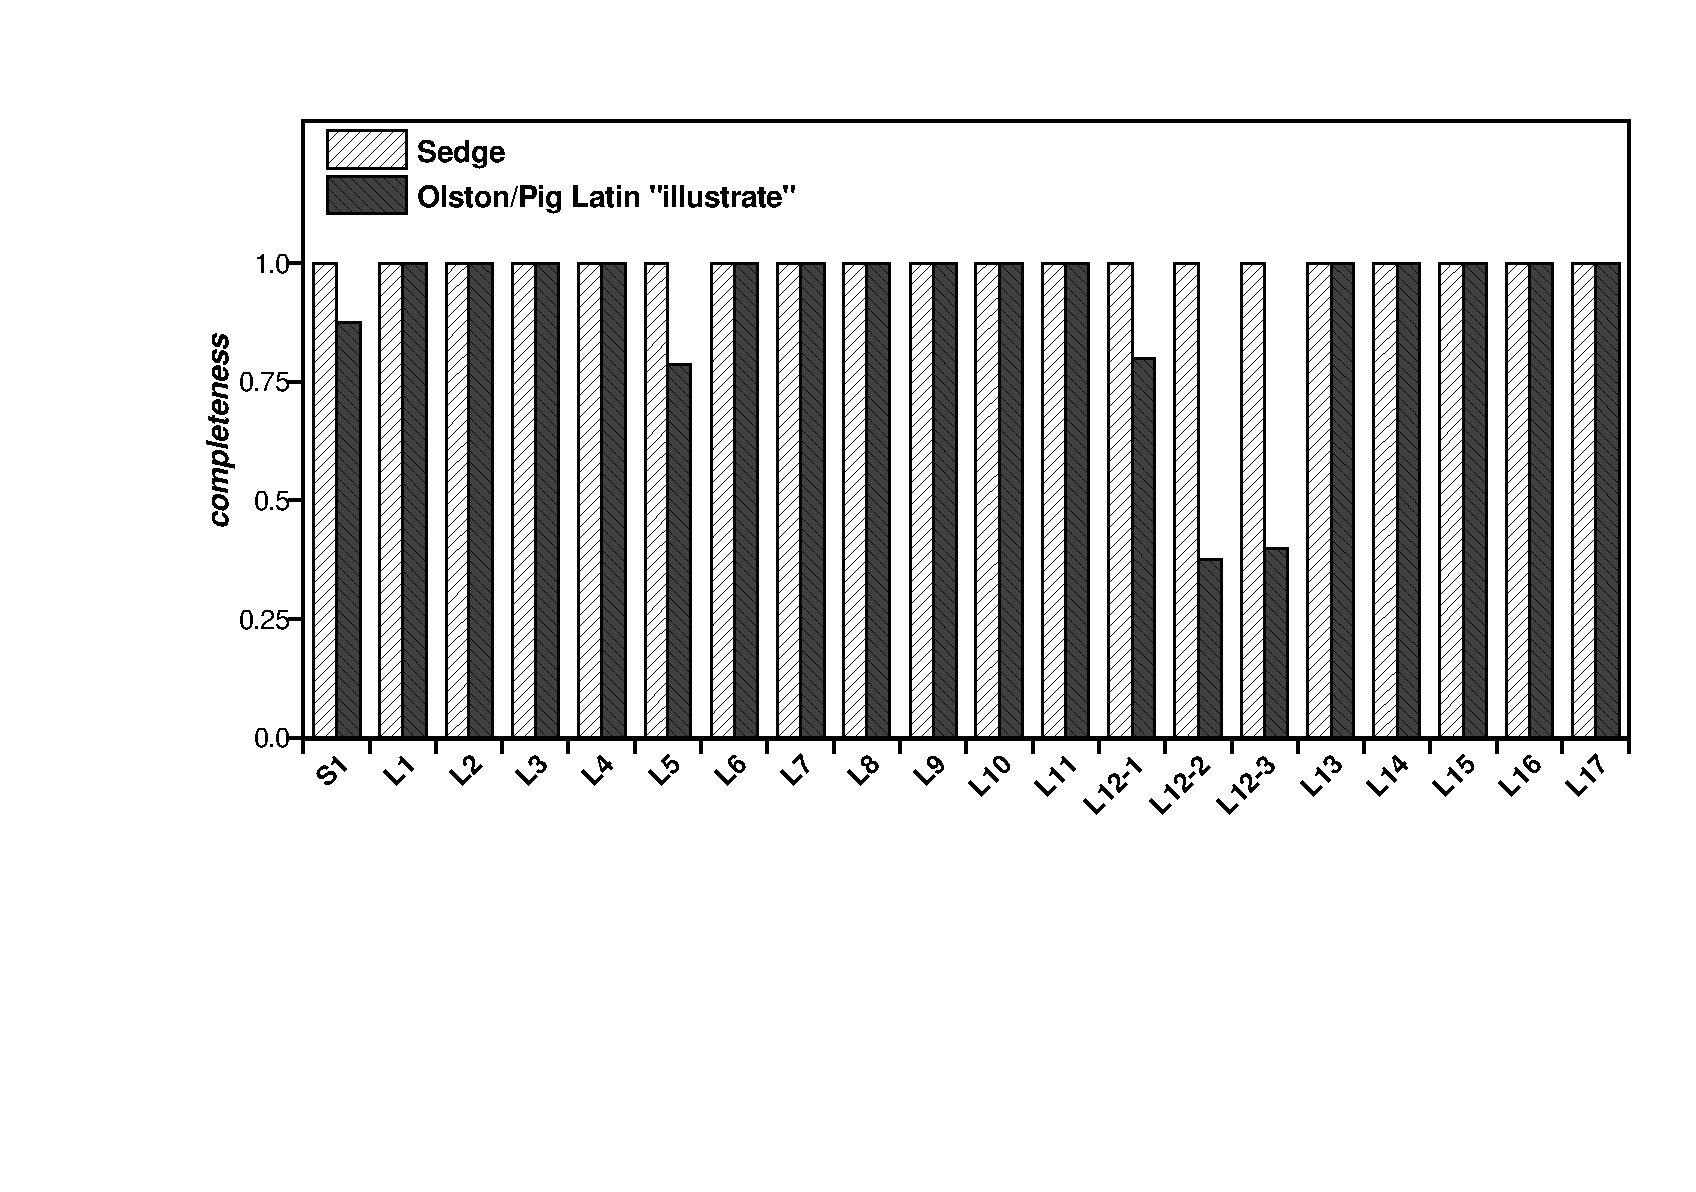
\includegraphics[scale=0.35]{CompletenessPigmix.pdf}}
\vspace{-70pt}
\caption{Completeness of sample data generation for the PigMix benchmarks}
\label{fig:pigmixC}
\end{figure}

%\cc{Figures~\ref{fig:pigmixC} and \ref{fig:sdssC}
%should only use a tiny amount of space, as
%the information density is currently very low. Each figure should 
%be single-column and take about 7 lines of vertical space.
%- Turn the x-tics to 90 degrees, not 45.
%- Move the shading legend inside the box.
%- Reduce the vertical space by 50\% at least.
%- You could replace the bars by simple dots (circle vs. x).}

\begin{figure}[ht]
\vspace{-20pt}
\centerline{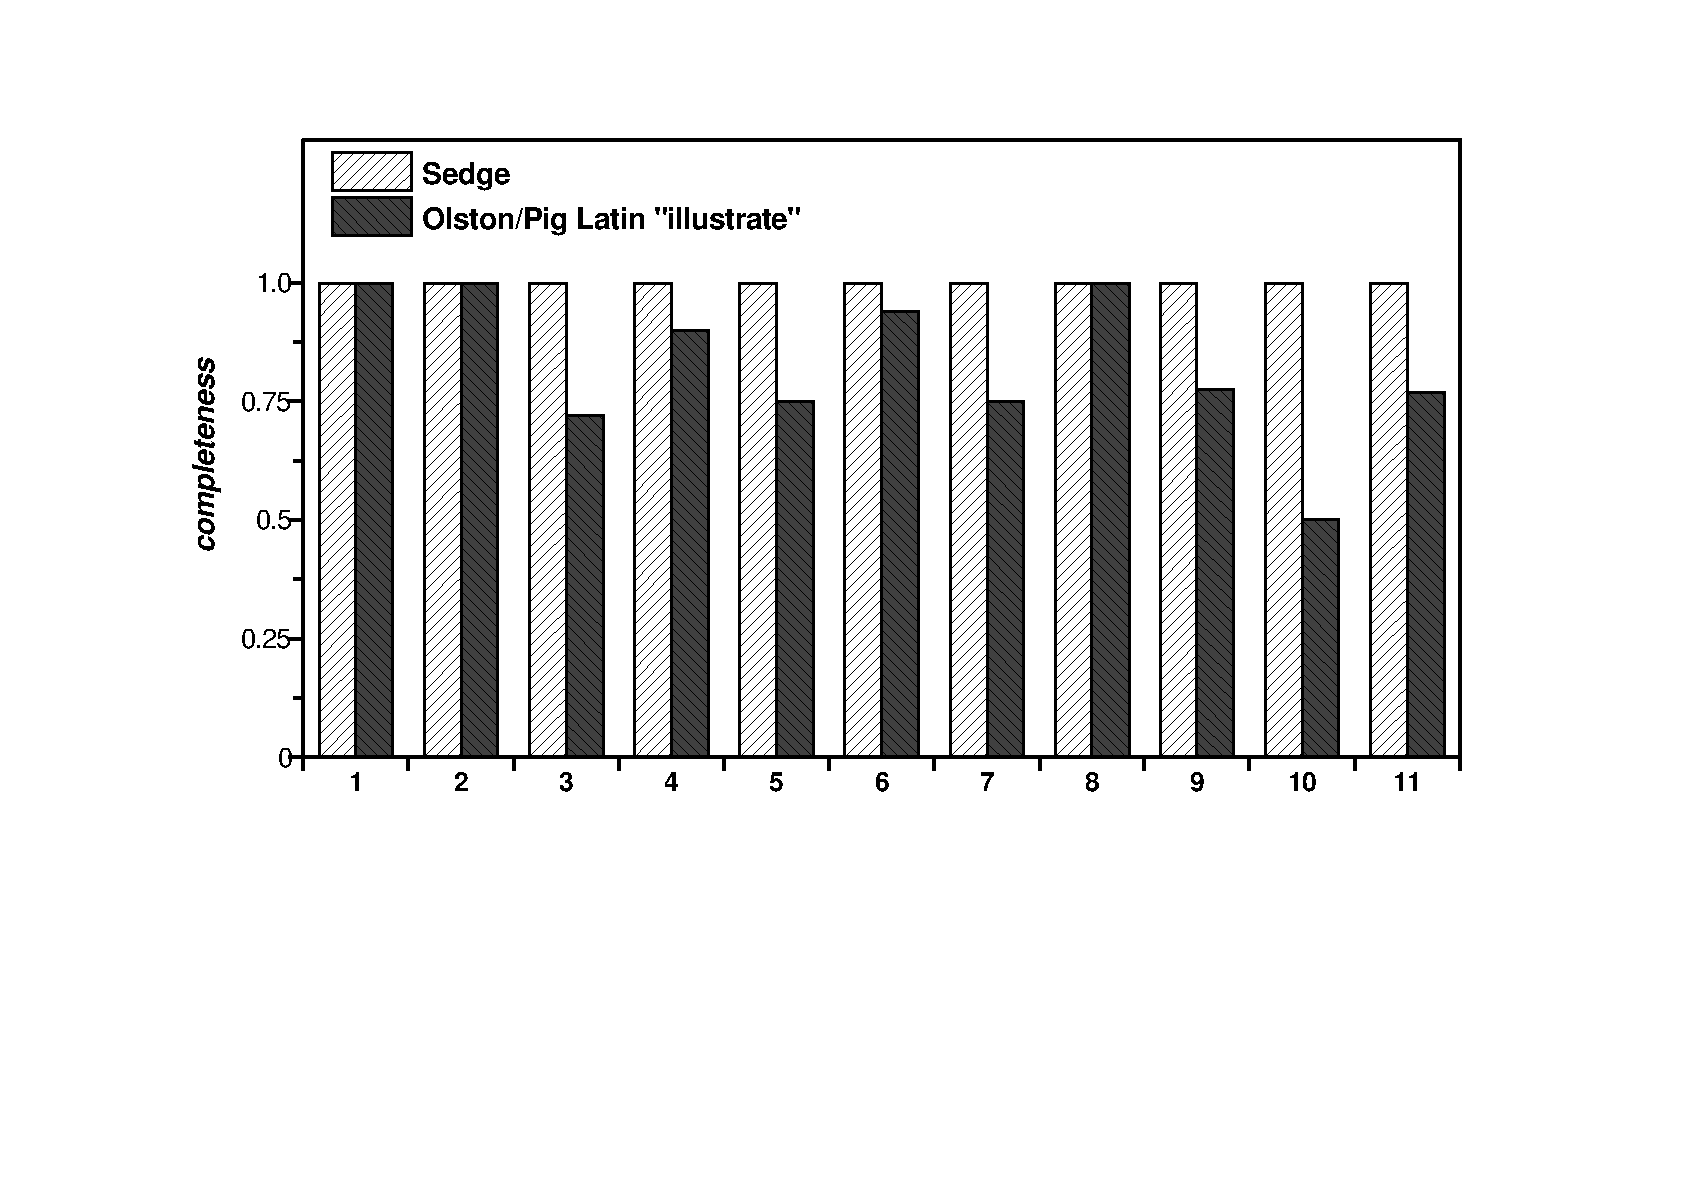
\includegraphics[scale=0.4]{CompletenessSDSS.pdf}}
\vspace{-85pt}
\caption{Completeness of sample data generation for the SDSS benchmarks}
\label{fig:sdssC}
\end{figure}

As can be seen, we improve on completeness for 5 out of 20 PigMix benchmark programs
and 7 out of 11 SDSS benchmark programs.  
Although the benchmark programs are small and much of their coverage
is achieved with random sampling of real inputs, they demonstrate
clearly the benefits of our approach. \emph{Practically every program in the
two benchmark sets that has any kind of complexity (either more than
one operator in the same path, or a user-defined function, or complex
filter conditions) is not fully covered by Olston's approach.}  For
example, Olston's system cannot generate data that fail the FILTER 
in the presence of grouping, projecting, UDF invocation
in the following program (program \emph{S1} in Figure~\ref{fig:pigmixC}).

\begin{lstlisting}[style=PigStyle, caption=PigMix program S1]
A = LOAD '$widerow' using PigStorage() 
  AS (name: chararray, c0: int, c1: int, ..., c31: int);
B = GROUP A BY name;
C = FOREACH B GENERATE group, SUM(A.c0) as c0, SUM(A.c1) as c1, ..., SUM(A.c31) as c500;
D = FILTER C BY c0 > 100 AND c1 > 100 AND c2 > 100 ... AND c31 > 100;
\end{lstlisting}

In fact, \textsc{Sedge} achieves perfect coverage (i.e., full completeness) for
all benchmark programs. 
Compared to Olston's approach our improved coverage is due to stronger
constraint solving ability (for programs \emph{4,5,6,7} in
Figure~\ref{fig:sdssC}), to UDF handling ability 
(for programs \emph{9,10} in Figure~\ref{fig:sdssC})
and also to inter-related constraints and global
reasoning (for programs \emph{S1,L5,L12-1,L12-2,L12-3} in
Figure~\ref{fig:pigmixC} and programs \emph{3,11} in
Figure~\ref{fig:sdssC}).

We also recorded how long it took \textsc{Sedge} and Olston's system to 
finish example generation.  We include the infrastructure
bootstrap time on each benchmark program.  Both 
\textsc{Sedge} and Olston's system need to prepare the Hadoop execution
environment for new executions.  \textsc{Sedge} needs to load 
its constraint solver Z3 and CORAL as well. 

As can be seen in Figure~\ref{fig:pigmixT} and Figure~\ref{fig:sdssT}, 
\textsc{Sedge} is faster on average than Olston's system in 18 out of 20 PigMix benchmark programs
and 9 out of 11 SDSS benchmark programs.  For the rest of
benchmark programs, \textsc{Sedge} incurs a little higher running time than 
Olston's system.  From these numbers we can infer that, 
although we have to conduct path exploration and constraint
solving, there are even time savings in most cases 
due to avoiding the step of pruning redundant tuples 
after the upstream pass (because our
approach does not generate redundant data).  
%\cc{Figures
%\ref{fig:pigmixT} and
%\ref{fig:sdssT}: There is a lot of white space. 
%- Shrink to 50\% of vertical space.
%- Consider replacing with tables.}

\begin{figure}[ht]
\vspace{-30pt}
\centerline{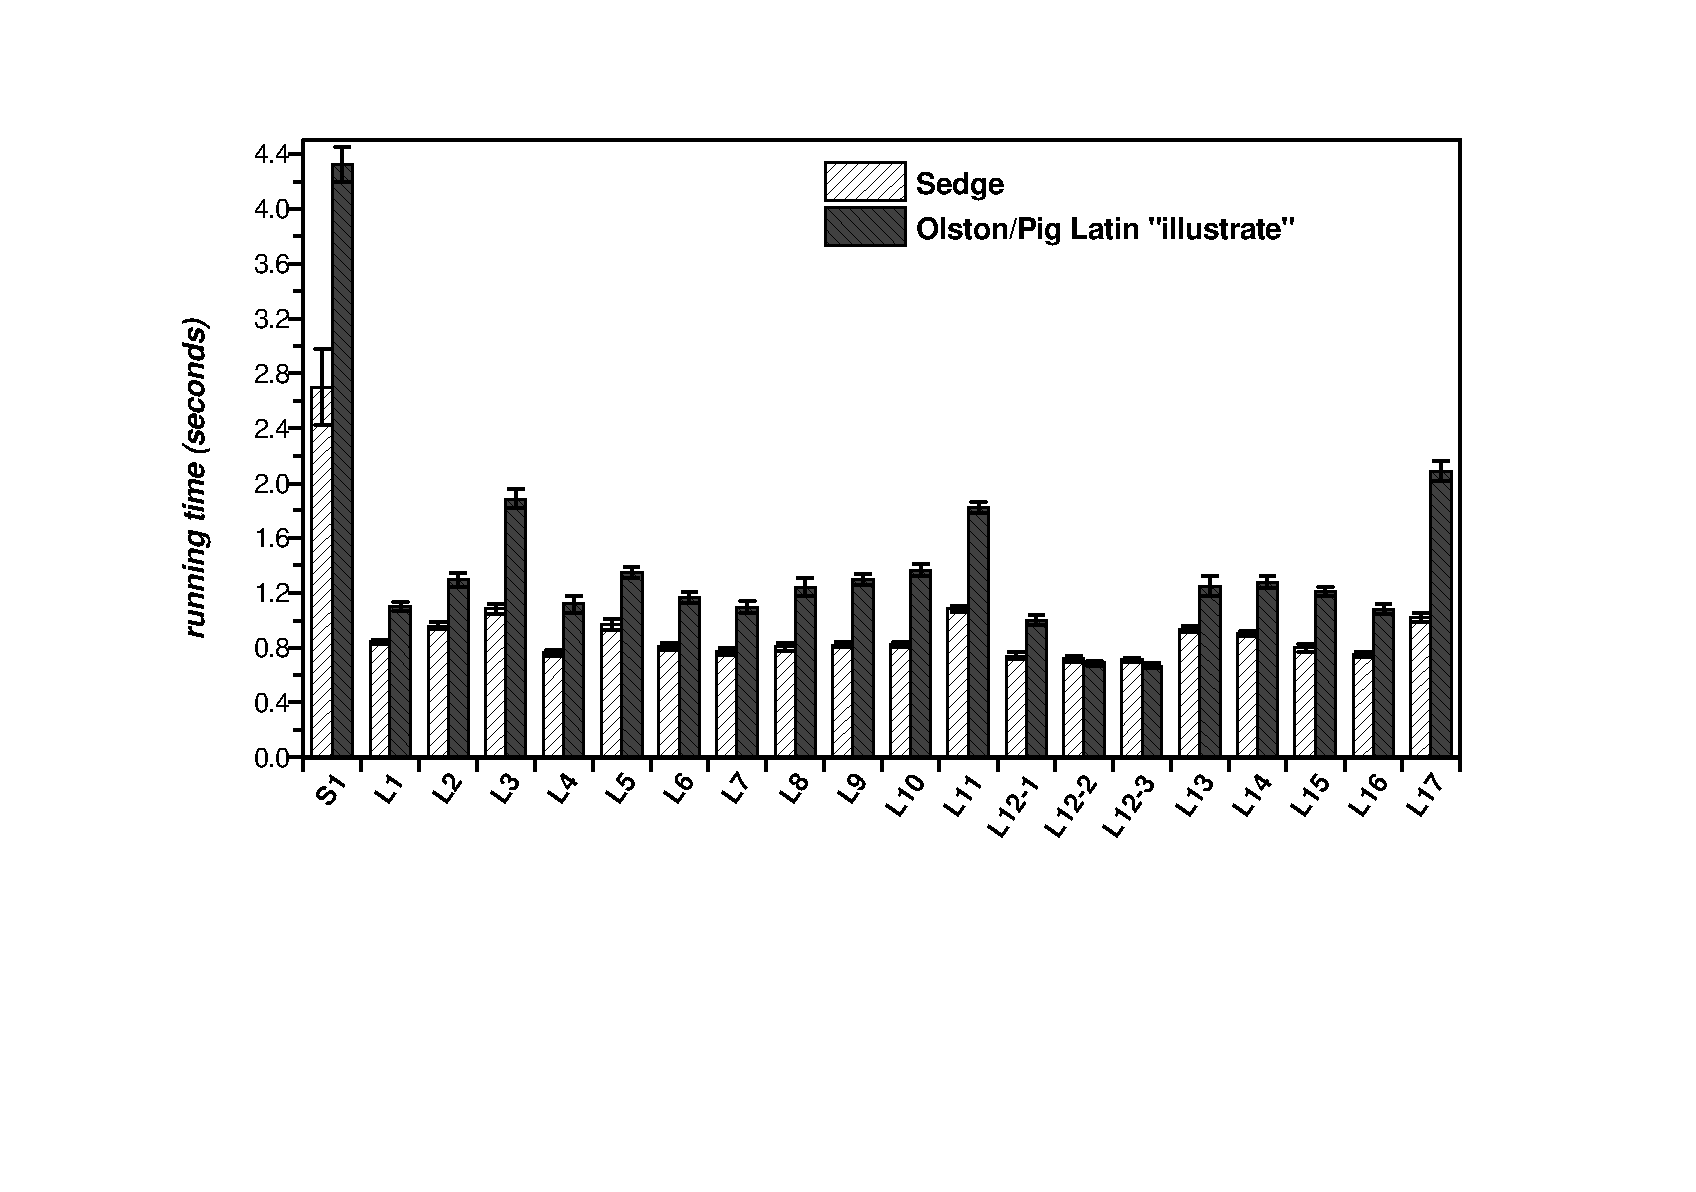
\includegraphics[scale=0.4]{TimePigmix.pdf}}
\vspace{-75pt}
\caption{Running time of sample data generation for the PigMix benchmarks}
\label{fig:pigmixT}
\end{figure}

\begin{figure}[ht]
\vspace{-30pt}
\centerline{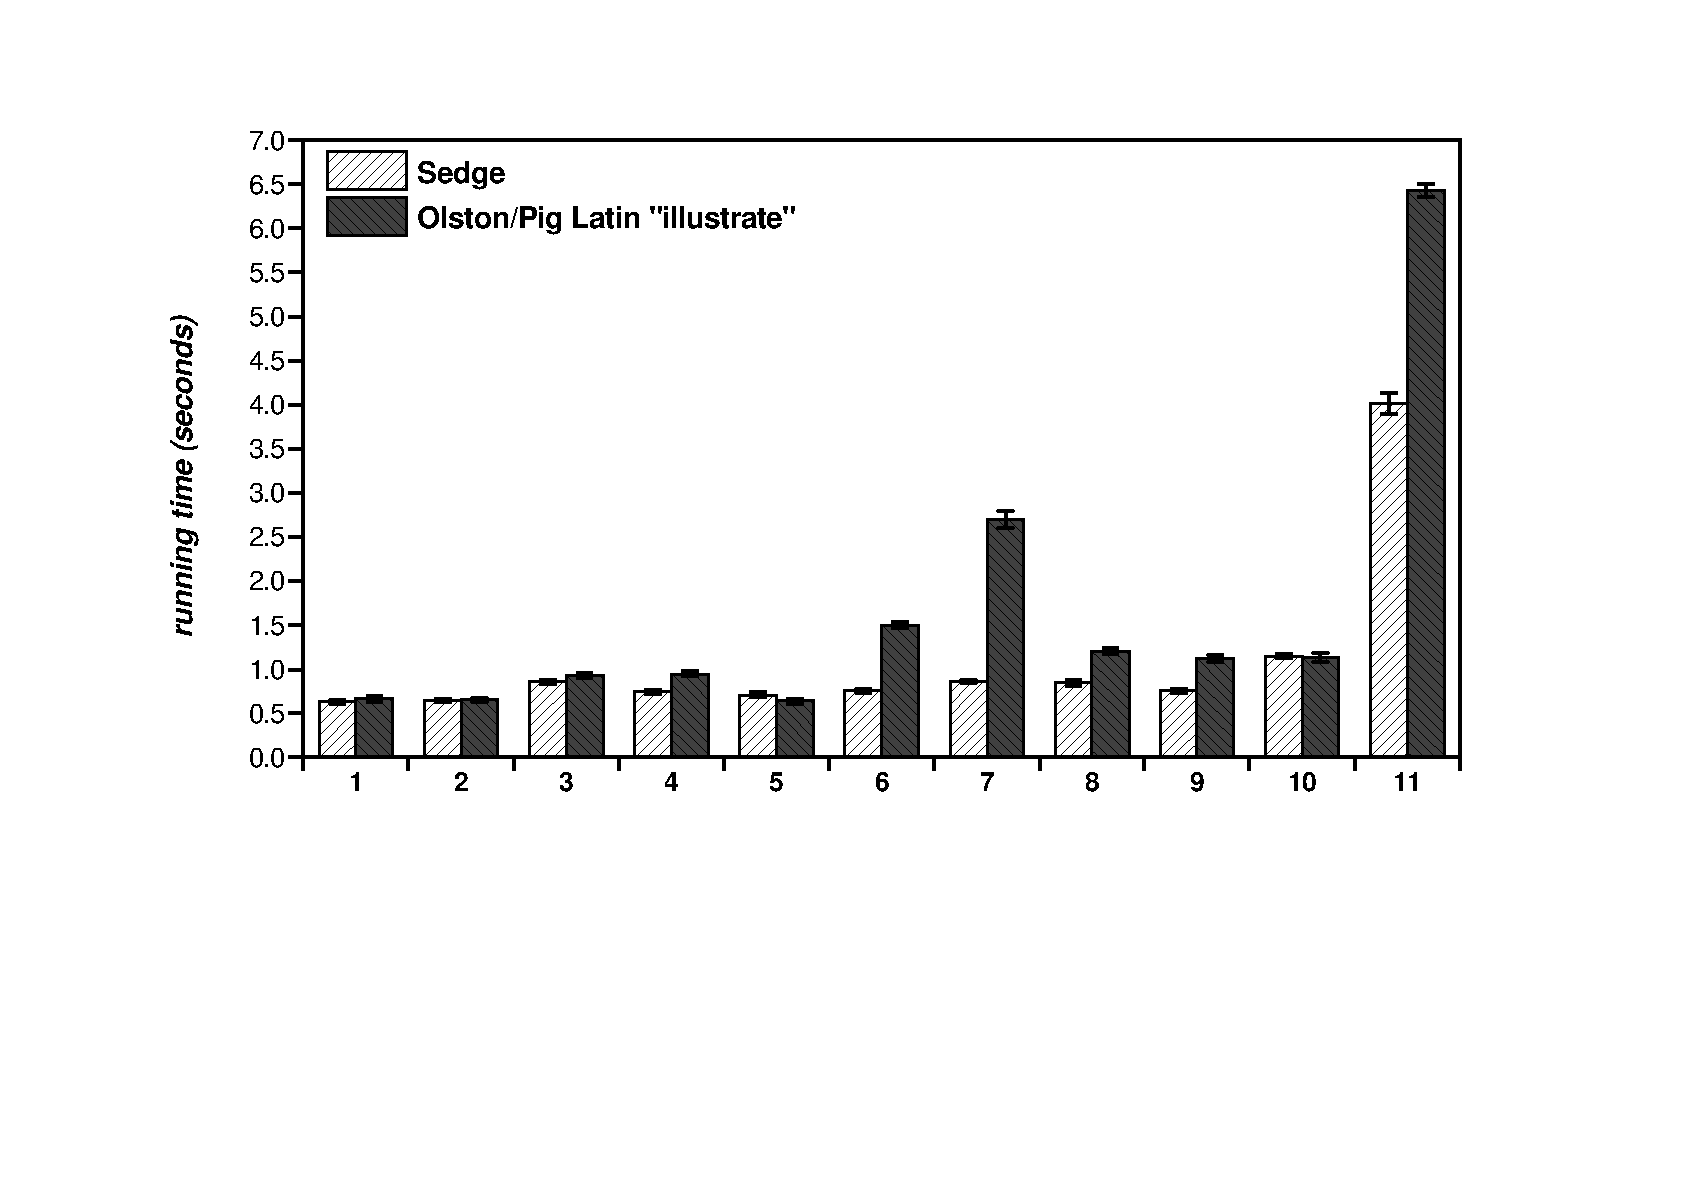
\includegraphics[scale=0.4]{TimeSDSS.pdf}}
\vspace{-85pt}
\caption{Running time of sample data generation for the SDSS benchmarks}
\label{fig:sdssT}
\end{figure}
%\subsection{Incremental analysis}
%\label{sec:eval-incremental}
%
%\begin{figure}[ht]
%\centerline{\includegraphics[scale=0.4]{2.pdf}}
%\caption{incremental}
%\label{fig:incremental}
%\end{figure}

%\subsection{Discussion}
%\label{sec:dis-benchmark-results}
%
%The example data generated by Olston's system has completeness score $1$, but its path coverage is otherwise low.

\section{Discussion: Why High-Level DSE}

%Although symbolic test data generation has not been applied before in
%the domain of dataflow languages, variations of the idea are in use
%in traditional imperative languages, in the form of dynamic-symbolic
%execution engines (e.g., Dart in C, jCute in Java, and Pex in
%C\#)~\cite{godefroid05dart,Tillmann:2008:PWB:1792786.1792798,Sen:2006:CJC:2135909.2135962}.
%We adapted the same idea to Pig, by producing constraints for the Pig
%Latin language constructs, as shown in Section~\ref{sec:design}.  The
%adaptation also changes the logical flow of the technique itself,
%however. Namely, the logical structure of our dynamic-symbolic
%execution engine is highly unconventional (compared to
%dynamic-symbolic execution engines for C, Java, or C\#).  Traditional
%dynamic-symbolic execution in C, Java, C\#, etc.  executes each
%concrete test case (given as part of the original input of the
%technique) in isolation. In the process of executing a test case that
%covers a branch of a conditional (e.g., the ``then'' condition of an
%``if-then-else''), the dynamic-symbolic engine tries to use the
%current state of the execution and only change the input variables so
%that the new data also cover the not-taken branch of the
%conditional. The need to keep the current state of the execution is
%important because complex side-effects could have taken place to
%create a global state that is consistent with the current execution
%point. In fact, dynamic-symbolic execution in imperative languages is
%powerful exactly because it avoids reasoning about complex state
%changes that took place since the starting point of the program's
%execution: the state is mostly inherited as-is from a real execution.
%
%In contrast, in our approach we first execute all concrete test
%cases, note their coverage and capture their behavior relative to
%complex expressions and user-defined functions. Then we produce
%symbolic constraints for each uncovered path in the dataflow program
%and combine this constraint with \emph{all} observations (over
%\emph{all} concrete paths) regarding complex expressions and
%user-defined functions. This represents the input to our
%constraint-solving engine, which outputs data to exercise the desired
%paths.
 
%The reason for the difference is dual. First, in dataflow languages
%there is no concept of side-effects. Data get processed through
%filters and combinators but there is no ``state of the execution'' to
%speak of. Second, in dataflow languages, data is king. Even a simple
%test case typically has inputs whose size dwarfs the size and
%complexity of the program itself. This means that it is doubly
%important to exploit concrete values that arise in real executions.
%Such concrete values are used as a hint for solving constraints that
%cannot be fully expressed symbolically or solved efficiently by our
%symbolic solver. These constraints include conditions on complex
%expressions (floating-point expressions, string and dates
%manipulation, etc.), as well as user-defined functions.
 
%More specifically, our setting contains no global mutable state. The
%tuples at every stage of an execution of a dataflow pipeline (e.g.,
%all the inputs to a specific ``filter'' operator) are a pure function
%of the original inputs of the program. This pure function cannot
%always be represented symbolically because it could contain
%user-defined operators or complex operators (e.g., floating point
%arithmetic), but it is still a function. This means that we can reason
%about all paths in parallel instead of exploring a single path and
%trying to alter it ``a little'' to produce others. In short, we can
%create compound symbolic constraints so that each one of them
%represents a single case of our desired coverage space. E.g., a
%symbolic constraint could represent ``data that pass the filter
% operator $F_1$, get joined with data that pass the filter operator
%$F_2$, so that the output fails (does not pass) filter operator
%$F_3$''. These constraints are similar to the ``path condition'' of a
%traditional symbolic execution (the conjunction of all conditions that
%gets us to the current program point). Yet our processing is still
%\emph{dynamic}-symbolic execution and not just symbolic execution
%because we use values from a concrete execution in two ways: First, we
%do not try to cover symbolically paths that are already covered by
%concrete values. Second, the concrete values are used to fix the
%behavior of unknown (e.g., user-defined) functions. If, for instance,
%a dataflow pipeline invokes an unknown function
%``\pig{function1(x,y)}'' and we observe dynamically that
%``\pig{function1(2,5) == 3}'' and ``\pig{function1(6,1) == 0}'', then we
% use these observations in our effort to solve the symbolic
%constraints, i.e., we encode these in the constraint solving process,
%thus allowing our solver to consider the possibility ``\pig{x == 2 && y
%  == 5 && function1 == 3}'' \emph{as well as} the possibility ``\pig{x
%  == 6 && y == 1 && function1 == 0}''. Because of the lack of
%side-effects, both of these possibilities can be considered
%simultaneously. In contrast, in dynamic-symbolic execution of an
%imperative program, only one value of an arbitrary user-defined
%function can be considered at a given constraint solving point.
%
%We summarize the above observation by saying that dynamic-symbolic
%execution of a dataflow program can do multiple-path analysis at
%once. Not only does a single symbolic constraint combine all
% conditions encountered in a path from input to final program output,
%but also the ability to solve a single symbolic constraint benefits
%from all other concrete executions. 
%
%\subsection{Comparison between \textsc{Sedge} and Pex}

A natural qualitative comparison is between a Dynamic Symbolic
Execution (DSE) engine at the level of the Pig Latin language and DSE
engines for imperative languages, since Pig Latin code is eventually
compiled into imperative code that uses a map-reduce library.  The
expected benefits from our approach are a) simplicity; b) conciseness
of the generated test cases (i.e., the same coverage with fewer
tests); and c) completeness: an imperative DSE engine may have trouble
solving constraints over the logically more complex generated code,
rather than the original Pig Latin code. Furthermore, an imperative
DSE engine cannot take advantage of the lack of side-effects in order
to better concretize user-defined functions, as discussed in
Section~\ref{sec:udf-recording}.


We compared \textsc{Sedge} with the Pex
\cite{Tillmann:2008:PWB:1792786.1792798} state-of-the-art DSE engine
in a limit study. Pex accepts \CS{} input, hence we hand-translated
Pig Latin programs into \CS{} programs.\footnote{Although there are
  DSE engines for Java---e.g., Dsc
  \cite{Islam:2010:DTC:1868321.1868326}---they do not match the
  industrial-strength nature of Pex. Dsc, for instance, does not
  support programs with floating point numbers, which are common in
  Pig Latin.}  The resulting \CS{} programs are single-threaded
without any call to the map-reduce API, in order to test the
applicability of Pex in the ideal case. (The inclusion of the
map-reduce library complicates the control-flow of the imperative
program even more and can easily cause the DSE engine to miss a
targeted branch of test execution, leading to low coverage of
generated test cases\cite{Xiao:2011:PIP:1985793.1985876}.)

For our translation, we inspected the Java code generated by the Pig
compiler and made a best-effort attempt to replicate it in \CS{},
without map-reduce calls. We translated 13 programs from our Pig Latin
benchmark suites. Since Pex has no knowledge of the original input (it
accepts concrete values only when passed into the test method as
parameters with primitive types) we enable just the 3rd pass (upstream
pass) of \textsc{Sedge}, for a fair comparison (i.e., \textsc{Sedge}
also does not benefit from sampled real data---this also disadvantages
\textsc{Sedge} as it removes the advantage of better UDF handling).

The results confirm our expectation. The conciseness of the test suite
generated by Pex is low since Pex needs to examine a lot of irrelevant
low-level branches or constraints that are not necessary for
equivalence class coverage of the high-level Pig Latin control flow.
% This is understandable as Pex is operating on
%a lower-level language, \CS{}, translated from a higher-level language,
%Pig Latin.  
For example, for step A in the Pig Latin program in
Listing~\ref{lst:sdss5}, Pex generates 30 tuples within 11 tables, of
which 3 tuples pass the filter in step B, while \textsc{Sedge}
generates 2 tuples within exactly 1 table, of which 1 tuple passes the
filter in step B.  The conciseness of the test suite generated by Pex
is 0.05, while the conciseness of the test suite generated by
\textsc{Sedge} is 0.75.  Furthermore, for specific complex constructs
we also get much higher completeness, although quite often Pex also gets
perfect coverage. In our experience, for Pig
Latin programs containing FILTER statements after (CO)GROUP or JOIN
statements, the test suites yielded by Pex lack in completeness.
For instance, in the SDSS program with 34 FILTER operations and 2 JOIN
operations, the Pex completeness is only 0.09.


%Our translation patterns are as follows. The
%input variables from LOAD are translated to the test method's
%parameters.  The output variables from STORE are translated to the
%test method's return variables.  In the case of FILTER, aggregate
%functions, and user-defined functions, we do basically a literal
%encoding of the MapReduce code that Hadoop would generate.  For
%example, as with Hadoop, we translate each FILTER A by P into either a
%foreach loop over all elements of A, filtering by P, or into an
%equivalent LINQ expression (which leads to very similar behavior of
%Pex).  In the case of GROUP and JOIN that have non-obvious translation
%like FILTER, we write LINQ code that is equivalent to what Pig Latin
%would have done.  In the case of UNION and COGROUP that have
%non-obvious translation like FILTER and have non-equivalent LINQ
%expression available, we write plain \CS{} code to simulate these
%operations.



%Making a fair comparison of \textsc{Sedge} and other dynamic symbolic
%execution (DSE) engines for traditional imperative languages is not
%straightforward.  One approach is to take Java Hadoop code translated
%by Pig and use DSE to generate test cases.  Unfortunately, as far as
%we know, very few Java DSE engines are publicly available.  In
%addition, most of these Java DSE engines could not be powerful enough
%to deal with real-world code bases.  For example, the Java DSE engine
%Dsc\cite{Islam:2010:DTC:1868321.1868326} does not support Java
%programs using floating-point numbers, which is common in Pig Latin
%programs. Another approach is to find a compiler to translate a Pig
%latin program into other semantically equivalent imperative language
%program that a target DSE engine can handle.  But such a full
%translation is not automated and is never complete.  Even if we can
%find a compiler to do a fair translation for a DSE engine, method
%calls to external libraries such as map-reduce API can easily cause
%the DSE engine to miss a targeted branch of test execution, leading to
%low coverage of generated test
%cases\cite{Xiao:2011:PIP:1985793.1985876}.  We want to compare
%\textsc{Sedge} with other DSE engines for imperative languages in
%terms of abstract reasoning and constraint solving.  We do not want
%method calls to MapReduce API introduced by compiler get in the way of
%symbolic reasoning for our purpose of comparison.
%
%
%Clearly, neither of the above two approaches can work. To compare
%\textsc{Sedge} and other DSE engines for traditional imperative
%languages requires careful benchmark construction.  We decide to
%manually translate a Pig Latin program into a single-threaded \CS{}
%program without any call to map-reduce API, and use Pex to generate
%test suites for the \CS{} program.  The map-reduce API call can be
%eliminated because map-reduce API calls are mostly about coordinating
%multiple machines to shuffle data between servers.  They have nothing
%to do with completeness.  Pex is by far the most mature DSE engine
%for an object-oriented language and currently in real use for .NET
%code.  The resulting \CS{} program is simpler than the code generated
%by Hadoop while still capturing the full meaning of the original Pig
%Latin program.  In this way, we have vastly reduced the complexity of
%the \CS{} code by eliminating the MapReduce overhead.  Hence, the \CS{}
%code is amenable to Pex to reason about.



%\begin{lstlisting}[style=PigStyle, caption=SDSS program 1]
%A = LOAD PhotoObj using PigStorage() AS (objID : long, field : int, ra : float, dec : float, run : int);
%B = FILTER A BY run == 1336 AND field ==11;
%\end{lstlisting}
%Pex would sometimes fail to achieve perfect completeness for Pig Latin programs containing UDF.  Consider the following program containing the UDF
%\textit{org.apache.pig.piggybank.evaluation.math.POW(double, double)} and \textit{org.apache.pig.piggybank.evaluation.math.SQRT(double)} (program \emph{10} in Figure~\ref{fig:sdssC}, shown with the UDF's name shortened).
%
%\begin{lstlisting}[style=PigStyle, caption=SDSS program 10]
%A = LOAD PhotoObj2 using PigStorage() AS (objID : long, rowv : double, colv : double);        
%B = FILTER A BY POW(rowv,2.0) + POW(colv, 2.0)) > 50.0 and rowv >= 0.0 and colv >=0.0;
%C = FOREACH B GENERATE SQRT(POW(rowv,2.0) + POW(colv, 2.0)) as velocity;
%\end{lstlisting}
%
%
%Pex fails to generate a tuple that can pass the FILTER in step B due to the presence of the UDF \textit{POW(double, double)}. This is a witness of concretization failure inside Pex.  \textsc{Sedge} can still achieve perfect completeness in this case by employing non-linear constraint solver Coral that can solve constraints with common numeric functions such as the power function and the square root function. 

%\section{Conclusions and Future Work}
%Generating example input data for dataflow programs has emerged as an
%important challenge. We presented \textsc{Sedge}: an approach and tool
%for generating example data of dataflow programs using DSE, 
%in order to achieve high coverage.  \textsc{Sedge}
%builds symbolic constraints over the equivalence classes induced by
%dataflow programming language constructs and can reason over
%constraints on user-defined functions by exploiting dynamic values as
%hints. We implemented our technique for the Pig dataflow system and
%compared it empirically with the most closely related prior work. 
%While we currently focus on the Pig Latin programming language, the principles are
%quite general.  The same high-level technique can be applied to other
%dataflow programming languages, such as
%DryadLINQ~\cite{Isard:2007:DDD:1272996.1273005} and
%Hyracks/Asterix~\cite{BehmBCGLOVDPT11}, and to relational algebra primitives, such
%as relational division and anti-join. 
%Our evaluation on third-party applications demonstrates that, with similar
%computing resources, our technique achieves better coverage of a given
%dataflow program.
%We described the first example input data generator 
%for dataflow programs that leverages dynamic symbolic program analysis. 

%The proposed \textsc{Sedge} approach has the limitation of path
%explosion as all other DSE approaches. The exponential growth of
%constraint generation will blow up constraint solvers and slow down
%the whole system significantly.  But since the Pig Latin programs we
%have seen so far are tens of lines in length, the limitation does not
%manifest itself.  For future work, we plan to study the support for a
%wider range of constraint solving optimizations
%\cite{Cadar:2013:SES:2408776.2408795} such as irrelevant constraint
%elimination and incremental solving, and consider to extend our
%techniques to allow for distributed dynamic symbolic execution
%\cite{Bucur:2011:PSE:1966445.1966463} for high performance.



%\section*{Acknowledgments}
%
%This material is based upon work supported by the National Science
%Foundation under Grants No. 1017305, 1117369, and IIS-1218524, and 
%funds from the UMass Science \& Technology Program. We also
%gratefully acknowledge funding by the European Union under a Marie
%Curie International Reintegration Grant and a European Research
%Council Starting/Consolidator grant; and by the Greek Secretariat for
%Research and Technology under an Excellence (Aristeia) award.
%
%Our tool is available at: \url{https://github.com/kaituo/sedge}.


%\chapter{Type Constraints}

\section{Introduction}
 Type constraints are logical formulas related to types. For example, the Java method header \java{void foo(List a)} implies the type constraint that the dynamic type of \java{a} is a subtype of \java{List}.  Without loss of generality, Sherman et al. \cite{Sherman:2015:DTP:2776776.2755971} finds 5 kinds of type constraints in Java programs:
 
\begin{enumerate}
    \item x $\preceq$ t: Variable type x is a subtype of constant type t. Example: From an if condition which uses \java{instanceof} to check if a given object \java{o} is a \java{Map} object, we can infer the type constraint \java{o} $\preceq$ Map.  
  \item x $\preceq$ y: Variable type x is a subtype of variable type y. Example: You might want to check if an object \java{o} is of type \java{clazz} via \java{java.lang.Class.isInstance()} like this: \java{clazz.isInstance(o)}. This expression contains the type constraint \java{o} $\preceq$ \java{clazz}.
  \item t $\preceq$ x: Constant type t is a subtype of variable type x. Example: When a method parameter \java{c} is constrained to satisfy the \java{java.lang.Class.isAssignableFrom()} constraint \java{c.isAssignableFrom(Integer.class)}, the actual type constraint is \java{Integer.class} $\preceq$ \java{c}.
  \item x $=$ y or x$\neq$ y: Variable type x equals to variable type y. The Java expressions such as \java{getClass().equals(other.getClass()} have been used to check whether one variable type equals to another variable type.
  \item x $=$ t or x$\neq$ t: Variable type x equals to constant type t. For example, Apache Hive \footnote{\url{https://github.com/apache/hive/blob/master/metastore/src/gen/thrift/gen-javabean/org/apache/hadoop/hive/metastore/api/ThriftHiveMetastore.java}} checks if a field's dynamic type equals to a constant type using a statement like \java{schemeField.type == org.apache.thrift.protocol.TType.STOP}.
\end{enumerate}


Type constraint reasoning is necessary as object oriented programming becomes prevalent.  A recent survey on open source applications with a total size of more than 2 MLOC by \cite{Islam14Generating} found three hundred cases of type constraints. Sherman et al. \cite{Sherman:2015:DTP:2776776.2755971} conducted experiments by collecting path constraints from dynamic symbolic execution. These path constraints include first-order logic formulas such as the numerical formula \java{a < 3} and the type constraint \java{a} is a subtype of \java{b}. It estimates that the average percentage of type constraints on five open source Java programs is 51\%.  

Type constraints have important application areas such as verification and testing. The official JVM spec \cite{Lindholm:2014:JVM:2636992} defines type constraints in Prolog to do type checking within Java compiler:``The type checker enforces type rules that are specified by means of Prolog clauses. English language text is used to describe the type rules in an informal way, while the Prolog clauses provide a formal specification.'' Another important application area of type constraints is dynamic symbolic execution, which often needs to create objects with correct types. Due to polymorphisms such as subtyping and dynamic dispatch, the dynamic type of a reference variable is often not equal to its declared static type. Various errors could arise if static types are to substitute dynamic types to create objects. With type constraints and a suitable constraint solver, we can easily find the correct dynamic type of an object. 

The challenge of type constraints reasoning is the analysis must be acceptably accurate not only in complete type hierarchy but also in incomplete type hierarchy while keeping the process at reasonable performance cost. Complete type hierarchy means all the required types are available in the search space. Incomplete type hierarchy means some types are missing in the search space either because the required classes have not been written (e.g. in the the test-driven development practice) or because the required classes have not been loaded yet (e.g. in languages like Java classes are loaded on demand).  

A streak of related work attempts to attack this challenge. SMT solver Z3's \cite{moura08Z3} official tutorial \footnote{\url{http://rise4fun.com/z3/tutorialcontent/guide}} provides a way of encoding type constraints using uninterpreted function.  With Z3 we have to assert the subtype relationship of every pair of x, y of types from known type systems. Sherman et al. \cite{Sherman:2015:DTP:2776776.2755971} finds that Z3 suffers severe performance degradation because of its huge number of asserted type constraints.  \cite{Islam14Generating} encodes ``subtype'' as a 2-dimensional array because they can tell Z3 to create an array whose fields are all ``false'' by default. Then they only have to assert actual subtypes. In other words, they do not have to assert ``X is not a subtype of A'', ``X is not a subtype of B'' etc. They only have to assert ``X is a subtype of C'', ``X is a subtype of D'' etc.  Still their algorithm has quadratic complexity.  For type constraints of the form x $\preceq$ t and x $=$ t, Sherman et al.'s solver \cite{Sherman:2015:DTP:2776776.2755971} is significantly faster than the two approaches mentioned above. But Sherman et al.'s solver is not able to solve the other 3 kinds of type constraints, including x $\preceq$ y, t $\preceq$ x and x $=$ y. We cannot ignore those 3 kinds of type constraints as they are common in projects.  Please see details of our case studies on the distribution of the 5 kinds of type constraints in Section~\ref{chp:case}. 

In this chapter, we describe an approach to reason about type constraints using Datalog. Datalog is a database query language that operates on relations (similar to tables in a database). Following predefined rules, new relations are computed based on projecting and joining existing relations as in relational database queries. Rules are usually in the form of implications. Our approach is guaranteed to have a polynomial complexity as the complexity class of Datalog is $P$ \cite{immerman2012descriptive}. In practice, our approach's time complexity is $O(n^2)$, where $n$ is the size of input relations.  This is because we compute unrelated input relations separately and we have rarely seen links among more than 2 relations.  Also, encoding type constraints using uninterpreted functions or arrays is slow due to its large number of asserted constraints. In contrast, Datalog makes a closed-world assumption and can define recursive rules, and the resulting type constraints are relatively smaller. A closed-world assumption treats anything that are not facts and cannot be inferred from existing facts as false. This assumption is convenient for type constraints encoding as we do not have to assert false or unknown relationships between two types: ``X is not a subtype of A'', ``X is not a subtype of B'' etc. Recursive rules are defined in a way that both body and head can contain the same relation.  This allows Datalog to instantiate new facts on demand. 

 declarative Datalog semantics

general 5 kinds of constraints

\section{Case Studies}
\label{chp:case}

 We have performed 4 case studies, searching for empirical evidence about the distribution of the 5 kinds of type constraints via the source code mining tool Boa \cite{Dyer-Nguyen-Rajan-Nguyen-13}. After analyzing 23,229,406 revisions, 7,830,023 projects of the September 2015 Github dataset available in Boa, we are able to find out the 5 kinds of type constraints are not evenly distributed, with the number of x $\preceq$ t constraints dominating the number of all other type constraints, but with other type constraints appearing in a similarly number of projects.  A caveat is some of the results may not be consistent with the programs, seemingly due to the semantic unsoundness in source code mining tools. For example, when there is a function call to \java{isAssignableFrom()}, Boa does not encode the receiver's static type. Therefore we cannot accurately determine type constraints in the function call to \java{java.lang.Class.isAssignableFrom()}.  

Our 4 case studies try to address the following research questions:

\textbf{(RQ1) How many expressions are matched with each kind of type constraints?}

While we found 69,338,416 expressions are matched with type constraints, 93.3\% of expressions contain x $\preceq$ t, as shown in Figure~\ref{fig:exprnumber}.

\textbf{(RQ2) In high quality projects, how many expressions are matched with each kind of type constraints?}

Ideally we want to use metrics like the number of downloads to measure the project quality.  But this information is not encoded by Boa.  Instead, we use the number of commits for a project as the quality metric: if a project has no less than 100 commits, we regard it as a high quality project. 

\textbf{(RQ3) How many projects are there where each kind of type constraints can be found at least once?}

There have been 164,998 projects with type constraints out of 7,830,023 projects in our dataset, according to Figure~\ref{fig:projectnumber}. We identified 63.2\% of those 164,998 projects have x $\preceq$ t expressions.  

\textbf{(RQ4) How many high quality projects are there where each kind of type constraints can be found at least once?}

Again, if a project has no less than 100 commits, we regard it as a high quality project. 




%\begin{figure*}[tb]
%\begin{center}
%\begin{scriptsize}
%\begin{tabular}{|l|r|r|r|r|r|r|r|r|r|}
%\hline
%&\multicolumn{3}{c|}{\textbf{isAssignableFrom}} & \multicolumn{3}{c|}{\textbf{isInstance}} & \textbf{instanceof} & \multicolumn{2}{c|}{\textbf{Equal}}  
%\\
%&x $<:$ t & t $<:$  x & x1 $<:$  x2 & x $<:$ t & t $<:$ x & x1 $<:$ x2 &x $<:$ t & x1 $=$ x2 & x $=$ t \\
%\hline
%\hline
%large & 1,001,478 & 178,340 & 527,760 & 194,303 & 25,054 & 513,570 &63,493,487& 1,711,876&1,692,548 \\
%%mc & 23 & 2/0 & 0/0 & 0/0 \\
%large & 12,247 & 4,075 & 9,365 & 2,949 &906 &8,193 &89,057&27,840&10,366 \\ 
%large& 4,566 & 1,735 & 3,655 & 1,193 &417&3,294&17,643&7,976&3,870 \\
%large & 882,098 & &&&&&57,704,965 & 1,495,999 & 1,617,767 \\
%\hline
%\end{tabular}
%\end{scriptsize}
%\end{center}
%\caption{Average running time in seconds for residual investigation on race 
%detection.}
%\label{fig:racetime}
%\end{figure*}

\begin{figure*}[tb]
\begin{center}
\begin{small}
\begin{tabular}{|l|c|c|c|c|c|}
\hline
& \multirow{2}{*}{x $\preceq$ t} &\multirow{2}{*}{t $\preceq$ x}& \multirow{2}{*}{x $\preceq$  y }& x $=$ y & x $=$ t
\\&&&&x$\neq$y&x$\neq$t\\
\hline
\hline
\textbf{isAssignableFrom} & 1,001,478 & 178,340 & 527,760 & n/a &n/a\\
\textbf{isInstance}&194,303 & 25,054 & 513,570&n/a&n/a\\
\textbf{instanceof} &63,493,487&n/a&n/a&n/a&n/a\\
\textbf{Equality}&n/a&n/a&n/a& 1,711,876&1,692,548 \\
%mc & 23 & 2/0 & 0/0 & 0/0 \\
\hline
\end{tabular}
\end{small}
\end{center}
\caption{Number of expressions that are matched with each kind of type constraints. For missing cells (``n/a''), the expression has no such type constraint. }
\label{fig:exprnumber}
\end{figure*}

\begin{figure*}[tb]
\begin{center}
\begin{small}
\begin{tabular}{|l|c|c|c|c|c|}
\hline
& \multirow{2}{*}{x $\preceq$ t} &\multirow{2}{*}{t $\preceq$ x}& \multirow{2}{*}{x $\preceq$  y }& x $=$ y & x $=$ t
\\&&&&x$\neq$y&x$\neq$t\\
\hline
\hline
\textbf{isAssignableFrom} & 882,098& 156,745 & 474,316 & n/a &n/a\\
\textbf{isInstance}& 169,096 & 20,018 & 474,588 &n/a&n/a\\
\textbf{instanceof} &57,704,965&n/a&n/a&n/a&n/a\\
\textbf{Equality}&n/a&n/a&n/a &1,495,999&1,617,767 \\
%mc & 23 & 2/0 & 0/0 & 0/0 \\
\hline
\end{tabular}
\end{small}
\end{center}
\caption{Number of expressions that are matched with each kind of type constraints in high quality projects. For missing cells (``n/a''), the expression has no such type constraint. }
\label{fig:exprnumber_quality}
\end{figure*}

\begin{figure*}[tb]
\begin{center}
\begin{small}
\begin{tabular}{|l|c|c|c|c|c|}
\hline
& \multirow{2}{*}{x $\preceq$ t} &\multirow{2}{*}{t $\preceq$ x}& \multirow{2}{*}{x $\preceq$  y }& x $=$ y & x $=$ t
\\&&&&x$\neq$y&x$\neq$t\\
\hline
\hline
\textbf{isAssignableFrom} & 12,247 & 4,075 & 9,365 & n/a &n/a\\
\textbf{isInstance}&2,949 &906 &8,193&n/a&n/a\\
\textbf{instanceof} &89,057&n/a&n/a&n/a&n/a\\
\textbf{Equality}&n/a&n/a&n/a&27,840&10,366 \\
%mc & 23 & 2/0 & 0/0 & 0/0 \\
\hline
\end{tabular}
\end{small}
\end{center}
\caption{Number of projects where each kind of type constraints can be found at least once.  For missing cells (``n/a''), the expression has no such type constraint. }
\label{fig:projectnumber}
\end{figure*}


\begin{figure*}[tb]
\begin{center}
\begin{small}
\begin{tabular}{|l|c|c|c|c|c|}
\hline
& \multirow{2}{*}{x $\preceq$ t} &\multirow{2}{*}{t $\preceq$ x}& \multirow{2}{*}{x $\preceq$  y }& x $=$ y & x $=$ t
\\&&&&x$\neq$y&x$\neq$t\\
\hline
\hline
\textbf{isAssignableFrom} & 4,566 & 1,735 & 3,655 & n/a &n/a\\
\textbf{isInstance}&1,193 &417&3,294&n/a&n/a\\
\textbf{instanceof} &17,643&n/a&n/a&n/a&n/a\\
\textbf{Equality}&n/a&n/a&n/a &7,976&3,870 \\
%mc & 23 & 2/0 & 0/0 & 0/0 \\
\hline
\end{tabular}
\end{small}
\end{center}
\caption{Number of high quality projects where each kind of type constraints can be found at least once.  For missing cells (``n/a''), the expression has no such type constraint. }
\label{fig:projectnumber_quality}
\end{figure*}

\section{Motivating example}

\begin{lstlisting}[style=JavaStyle, caption=An example Java program, label=lst:motivation]
static public void invokeInterface(I i) {
    new C1();
    new C2();
    int res = i.foo(0); 
    
    Goals.reached(0);
    
    if (res == 1)
      Goals.reached(1);

    else if (res == 2)
      Goals.reached(2);
    
    else
      Goals.reached(3);   
  }

\end{lstlisting}

\chapter{Related Work}
\label{chp:related}

There is a lot of interesting work on the three different research
directions covered by this dissertation. This chapter discusses 
representative work for each area as belows.

\section{Residual Investigation: Predictive and Precise Bug Detection}

% The proposed analysis is a light-weight static-dynamic combo that produces warnings that are more actionable than FindBugs warnings but not quite as actionable as a test case that exhibits the actual bug:
% 1) Run FindBugs hashCode--equals detector
% 2) Detector flags some classes as inconsistent
% 3) Detector installs dynamic check in these classes
% 4) If program (during testing, deployment) adds instance of such class into a data structure: Warning

Static and dynamic analyses are routinely chained together for
checking program correctness conditions in programming languages,
i.e., in compilers and runtime systems. Compilers check certain
properties statically and insert runtime checks for remaining
properties. A classic example is checking that an array read does not
access a memory location outside the bounds of the array. To enforce
this property, Java compilers traditionally insert a dynamic check
into the code before each array read. To reduce the runtime overhead,
static analyses such as ABCD~\cite{bodik00abcd} have been developed
that can guarantee some reads as being within bounds, so that only the
remaining ones have to be checked dynamically. Beyond array
bounds checking, a similar static dynamic analysis pipeline has been
applied to more complex properties. The Spec\# extended compiler
framework~\cite{barnett04spec} is a prime example: it can prove some
pre- and post-conditions statically and generates runtime checks for
the remaining ones. 
Gopinathan and Rajamani \cite{Gopinathan:2008:EOP:1449764.1449784} use a combination of static
and dynamic analysis for enforcing object protocols. Their approach
separates the static checking of protocol correctness from a
dynamic check of program conformance to the protocol.

In residual dynamic typestate analysis, explored by Dwyer and Purandare
\cite{dwyer07residual}, Bodden \cite{bodden10efficient} and Bodden et al.
\cite{bodden07staged}, a dynamic typestate analysis that monitors all
program transitions for bugs is reduced to a residual analysis that
just monitors those program transitions that are left undecided by a
previous static analysis. This approach exploits the fact that a
static typestate analysis is typically complete, i.e., it
over-approximates the states in which a program can be. If for a small
sub-region of the program the over-approximated state sets do not
contain an error state, all transitions within such a region can
be safely summarized and ignored by the subsequent residual
dynamic analysis. At a high level, our approach adopts this idea, by
only monitoring those aspects of the program that the static analysis
has flagged as suspicious. However, our approach is more general in
two dimensions, (1) typestate analysis is restricted to verifying
finite state machine properties (``do not pop before push''), while
our approach can be applied to more complex properties (``do not pop
more than pushed'') and (2) our dynamic analysis is predictive: it
leverages dynamic results to identify bugs in code both executed and
not executed during the analysis.
% In typestate analysis the program correctness criterion is a finite state automaton, some program actions trigger transitions in the automaton and some transitions lead to an error state. The results of the static analysis are used to minimize the automaton checked by the dynamic analysis. Short follow-up SPIN paper on residual checking of safety properties~\cite{dwyer08residual}.

Beyond typestates, the idea of speeding up a dynamic program analysis
by pre-computing some parts statically has been applied to other
analyses, such as information flow analysis. For example, recent work
by Chugh et al. \cite{chugh09staged} provides a fast dynamic
information flow analysis of JavaScript programs. JavaScript programs
are highly dynamic and can load additional code elements during
execution. These dynamically loaded program elements can only be
checked dynamically. Their staged analysis statically propagates its
results throughout the statically known code areas, up to the borders
at which code can change at runtime. These intermediate results are
then packaged into residual checkers that can be evaluated efficiently
at runtime, minimizing the runtime checking overhead.

Our analysis can be seen in a similar light as residual dynamic typestate analysis and residual information flow analysis. If we take as a hypothetical baseline somebody running only our residual checkers, then adding the static bug finding analysis as a pre-step would indeed make the residual dynamic analysis more efficient, as the static analysis focuses the residual analysis on code that may have bugs. However, our goals are very different. Our 
real baseline is an established static analysis technique whose main problem is over-approximation, which leads to users ignoring true warnings. 

Check'n'Crash~\cite{csallner05check} and DSD-Crasher~\cite{csallner06dsd-crasher,smaragdakis07combining} can be seen as strict versions of residual analysis. These earlier techniques share our goal of convincing users of the validity of static bug warnings. However, Check'n'Crash and DSD-Crasher guarantee that a given warning is true, by generating and executing concrete test cases that satisfy the static warning, until a static warning can be replicated in a concrete execution or a user-defined limit is reached. While such proof is very convincing, it also narrows the technique's scope (i.e., these tools could only confirm very few warnings). In our current residual investigation, we relax this strict interpretation and also consider predictive clues that are likely to confirm a static warning.

We have already mentioned dynamic symbolic execution in Section~\ref{sec:staticdynamic} and Chapter~\ref{chp:sedgepaper}: a combination of concrete and symbolic execution. Similar to Check'n'Crash~\cite{csallner05check} and DSD-Crasher~\cite{csallner06dsd-crasher,smaragdakis07combining}, dynamic symbolic execution is also a strict approach that warns a user only after it has generated and executed a test case that proves the
existence of a bug. Compared to our analysis, dynamic symbolic
execution is heavier-weight, by building and maintaining
during program execution a fully symbolic representation of the
program state. While such detailed symbolic information can be useful
for many kinds of program analyses, our current residual
investigations do not need such symbolic information, making our
approach more scalable.

Monitoring-oriented programming (MOP)~\cite{chen07mop} shows how
runtime monitoring of correctness conditions can be implemented more
efficiently, even without a prefixed static analysis. JavaMOP, for
example, compiles correctness conditions to Java aspects that add
little runtime overhead. This technique is orthogonal to ours,
as some of our dynamic analyses are implemented manually
using AspectJ. Expressing them in terms of JavaMOP would be a
straightforward way to reduce our runtime overhead.

Our analysis can be viewed as a ranking system on static analysis
error reports.  There has been significant work in this direction using data mining.
Kremenek et al. \cite{kremenek2004} sort error reports by their probabilities.  A
model is used for computing probabilities for each error report by
leveraging code locality, code versioning, and user feedback.  The
effectiveness of the model depends on (1) a fair number of reports and
(2) strong clustering of false positives.  Kim and Ernst \cite{kim2007} prioritize
warning categories by mining change log history messages.
Intuitively, they expect a warning category to be important if warning
instances from the category are removed many times in the revision
history of a system. Their method requires change logs of good
quality. For static tools such as FindBugs, which analyze Java
bytecode to generate warnings, they also require compilation of each
revision. Bodden et al. \cite{Bodden2008FPE} use a machine-learning approach to filter out false positives of their static analyses for validating a finite state property.  They identify cases where imprecise static analysis information can appear due to factors such as dynamic class loading and interprocedural data flow.  They then use each case as a feature for decision tree learning.  The key difference between our approach and data-mining-based ones is that our approach considers the possible objections to static error reports.  As a result, we can validate more complicated error situations that require understanding what a programmer has in mind in practice when writing their code. 

Besides Eraser~\cite{266641}, some other related work on race detection comes under the label of predictive race analysis.  
%reports a race whenever two threads access the same memory location without holding a common lock and one of the access is a write. 
Chen and Rosu \cite{Chen:2007:PSC:1770351.1770387} predict races by logging only relevant information in a program trace and then model-checking all feasible trace permutations.   jPredictor \cite{Chen:2008:JPR:1368088.1368119} present a polynomial algorithm that can search a thread scheduling for a potential race that did not occur in the observed execution. jPredictor is not sound.  Smaragdakis et al. \cite{Smaragdakis:2012:SPR:2103656.2103702} define the causally-precedes relation (CP) that weakens the traditional Happens-Before relation.  The CP approach can generalize beyond an observed execution and guarantee soundness and polynomial complexity. These sophisticated predictive approaches can offer greater precision than residual investigation in terms of race detection, whereas our residual investigation based race detector can have fewer false negatives, due to the better coverage of static analysis tools and the conservativeness of our dynamic analysis.

The precision of bug detection software can be greatly enhanced with
human supervision at residual steps.  After an automated static
program verification step, Dillig et al. \cite{Dillig:2012:AED:2254064.2254087}
rely on humans to help reduce false positives by asking humans simple
and relevant questions.  Xie \cite{Xie2012SCAM} proposes to use humans to
guide otherwise intractable problems faced by test case
generators.  Combining such techniques in our approach would be interesting.  For instance, residual investigation's precision is
influenced by the native test suite coverage.  With the help of human
users, additional test cases can be constructed if required.


\section{Second-Order Constraints in Dynamic Invariant Inference}

There is a wealth of other work on invariant inference. We next
selectively focus on some recent approaches that were not covered in
the body of the paper (typically because they focus on static
invariant inference techniques).

For reverse engineering, Gannod and Cheng \cite{gannod95strongest}
proposed to infer detailed specifications statically by computing the
strongest postconditions. Nevertheless, pre/postconditions obtained
from analyzing the implementation are usually too detailed to
understand and too specific to support program evolution. Gannod and
Cheng \cite{gannod99specification} addressed this deficiency by
generalizing the inferred specification, for instance by deleting
conjuncts, or adding disjuncts or implications. Their approach
requires loop bounds and invariants, both of which must be added
manually.

There has been some recent progress in inferring invariants using
abstract interpretation. Logozzo \cite{logozzo04automatic,logozzo-phd}
infers loop invariants while inferring class invariants.  The
limitation of his approach are the available abstract domains;
numerical domains are best studied. Resulting specifications are
expressed in terms of fields of classes. 

Flanagan and Leino \cite{flanagan01houdini} propose a lightweight
verification-based tool, named Houdini, to statically infer ESC/Java
\cite{flanagan02extended} annotations from unannotated Java
programs. Based on pre-set property patterns, Houdini conjectures a
large number of possible annotations and then uses ESC/Java to verify
or refute each of them. The ability of this approach is limited by the
patterns used. In fact, only simple patterns are feasible, otherwise
too many candidate annotations will be generated, and, consequently,
it will take a long time for ESC/Java to verify complicated
properties.

Taghdiri \cite{10.1109/ASE.2004.10075} uses a counterexample-guided
refinement process to infer over-approximate specifications for
procedures called in the function being verified. In contrast to our
approach, Taghdiri aims to approximate the behaviors for the
procedures within the caller's context instead of inferring
specifications of the procedure.

Henkel and Diwan \cite{henkel07discovering} have built a tool to
dynamically discover algebraic specifications for interfaces of Java
classes. Their specifications relate sequences of method invocations.
The tool generates many terms as test cases from the class
signature. The results of these tests are generalized to algebraic
specifications.  They use a second tool to dynamically compare
their specifications against implementations by executing both
simultaneously and comparing their behavior \cite{henkel08debugging}.

Much of the work on specification mining is targeted at inferring API
protocols dynamically.  Whaley et al. \cite{whaley-automatic} create 
a finite state machine into which a transition from method A to 
method B is added if the post-condition of method A is not mutually
exclusive with the pre-condition of method B. 
%describe a system to extract component interfaces as finite 
%state machines from execution traces. 
Meghani and Ernst \cite{MeghaniE2003} build upon Whaley's work by 
using Daikon to determine the likely pre/post-condition of each method.
Other approaches use data mining techniques.  For
instance Ammons et al. \cite{ammons02mining} use a learner to infer
nondeterministic state machines from traces; similarly, Yang and Evans
\cite{996832} built Terracotta, a tool to generate regular patterns
of method invocations from observed runs of the program. Li and Zhou
\cite{1081755} apply data mining in the source code to infer
programming rules, i.e., usage of related methods and variables, and
then detect potential bugs by locating the violation of these rules.
Gabel and Su \cite{Gabel:2010:OIE:1806799.1806806} dynamically 
infer and verify method call ordering constraints, and
report the constraints only if they are violated. 
Beschastnikh et al. \cite{Beschastnikh:2011:LEI:2025113.2025151} 
use mined temporal invariants from logs to derive a refined
finite state machine. 
Although not explicitly our goal, some of our second-order constraints
can be thought of
as a way to express temporal API protocols.
For example, we can find the general has$\ast$, next$\ast$ type
specification \cite{Gabel:2010:OIE:1806799.1806806} by checking if \emph{CanFollow(has$\ast$(return==true),next$\ast$)},
or that the postcondition of has$\ast$ when has$\ast$ 
returns true implies the precondition of next$\ast$.  
It is interesting future work to see how to integrate 
existing techniques on specification mining with our approach 
to derive automata that describe correct behavior.

\section{SEDGE: Symbolic Example Data Generation for Dataflow Programs}
%PL&SE

Dataflow languages such as Pig can be seen as a compromise between
declarative languages, such as SQL, and imperative languages, such as C
and Java. That is, Pig combines the declarative feature of
straightforward parallel computation with the imperative feature of
explicit intermediate results. 
%However, besides the work by Olston et
%al.~\cite{Olston:2009:GED:1559845.1559873}, with which we have
%compared in detail in Section
%%s~\ref{sec:background_olston} and~
%\ref{sec:eval}, we are not aware of any related work that
%addresses test data generation for dataflow languages. 
There is little work (discussed in earlier sections) that addresses
test data generation for dataflow languages. Instead, the
related work from various research communities has focused on the
extreme ends of this spectrum, i.e., either on SQL or Java-like
programming languages.

Specifically, related work in the software engineering community has
focused on traditional procedural and object-oriented database-centric
programs, tested via combinations of static and dynamic reasoning
\cite{DBLP:conf/tap/SmaragdakisC07}. The main approaches use static
symbolic execution~\cite{marcozzi12test} or dynamic symbolic
execution~\cite{emmi07dynamic,li10dynamic,pan11generating}.  While our
work is inspired by such earlier dynamic symbolic execution
approaches, we adapted this work to dataflow programs and their
execution semantics. At the other end, there is work that
automatically generates database data that satisfy external
constraints \cite{orm-ase07} but there is no coverage or conciseness
goal and no application to dataflow languages. Another work
\cite{tuya10full} has introduced the idea of code coverage to SQL
queries. For our purposes, we reused the concept of coverage for Pig
Latin as defined by Olston et al.
\cite{Olston:2009:GED:1559845.1559873}.

%\cite{Khalek:2011:STD:1989760.1990071}
%% CC says: tuya10full applies the SE idea of code coverage to SQL queries.

In the formal methods community, Qex is generating test inputs for SQL 
queries~\cite{veanes10qex}. Similar to our work, Qex maps a SQL
query to SMT and uses the Z3 constraint solver to infer data tables.
However, Qex differs from our work in that Qex does not have a dynamic 
program analysis component and therefore cannot observe how a query
processes existing example data. Earlier work in the software engineering
community on dynamic symbolic execution has shown that dynamic analysis
can make such program analysis more efficient and enable it to reason
about user-defined functions, which we leverage in our work.

%% CC says: It is probably not worth to distinguish here between
%% generating program inputs that merely select data from an existing db
%% \cite{li10dynamic,pan11generating} 
%% and synthesizing fresh db data (that may not correspond to any ``real'' 
%% db data) \cite{emmi07dynamic,marcozzi12test}.
%% CC says: 
%% - li10dynamic generates a SQL query as a program input, given a db state
%% - pan11generating generates general program inputs, given a db state
%% - marcozzi12test maps individual CFG-paths to Alloy constraints.
% \todo{YL: What is the technical difference from our work?}
%\todo{YL: Is this survey complete?}
%\cc{Nothing else comes to mind, but I will make another pass.}

%% CC says: karam01testing,karam08unit define coverage criteria for
%% (visual) dataflow languages: all-nodes, all-edges, and def-use.


%DATABASES
%(1) DB testing
In the database community, a common methodology for testing a database
management system or a database application is to generate a set of
test databases given target query workloads.  Overall our problem
differs in that, instead of a whole database, we aim to generate a
small (or minimum if desired) set of tuples that have perfect path
coverage of a given dataflow program.  The recent work on reverse
query processing~\cite{binnig07reverse} takes an application query and
a result set as input, and generates a corresponding input database by
exploiting \textit{reverse relational algebra}. In comparison, our
work focuses on dataflow programs for big data applications, where
many operators are non-relational, e.g., map(), reduce(), and
arbitrary user-defined functions, and hence a ``reverse algebra'' may
not exist.  The QAGen system~\cite{BinnigKLO07} further takes into
account a set of constraints, usually cardinality and data
distribution in input and operator output tables, and aims to generate
a database that satisfies these constraints. Analogously to earlier
work in the formal methods community, this work performs a static
symbolic analysis and does not obtain additional information from a
dynamic analysis.
%% CC says: Do we really need to discuss QAGen? These authors' other
%% work on reverse query processing (binnig07reverse) is more closely
%% related to our work.
%
%%YS: Removed both paras below for space.
%More recent work, including~\cite{Lo:2010:GDQ} and \cite{Arasu:2011:DGU}, proposes to generate databases with approximate cardinalities  for im%proved performance, but those approximation techniques are not directly relevant to our work.
%%% There is some similar work in the SE community, i.e.:
%% Testing DBMS using Alloy~\cite{khalek11systematic}.

%(2) applications of data examples 

%More broadly, data examples have been employed to assist in schema
%mapping~\cite{Alexe:2010:CSM,Alexe:2011:DRS}. But this line of work
%addresses a different question: given a finite set of data examples,
%it decides whether or not there exists a schema mapping specified by
%global and local view constraints t%hat ``fits'' these data examples.


%%%This section needs to be moved to the section of rfbi's related work.
\section{Providing dynamic symbolic execution with concrete system states}

Similar to us, hybrid concolic testing\cite{Majumdar:2007:HCT:1248820.1248874} interleaves random testing and concolic testing to increase coverage.  The switch from random testing to concolic testing happens when random testing does not find new coverage points after a predetermined steps; the switch from concolic testing to random testing happens when concolic testing finds an input to an uncovered branch goal (though concolic testing may need to explore several feasible execution paths to generate the new input).  But hybrid concolic testing is not designed to trigger one specific bug condition.  We are targeting at generating tests to trigger one specific bug condition, using call graph search and dynamic symbolic execution. 

\cite{Elbaum:2006:CDU:1181775.1181806} saves system test states and restores those states as regression tests.  We also save system test states.  But our purpose is helping setting up environment (i.e. assignments to heap variables) for starting dynamic symbolic execution of the “switching” method.

The closest work to us is \cite{Pasareanu:2008:CUS:1390630.1390635}, which uses system tests to set up the environment.  Different from\cite{Pasareanu:2008:CUS:1390630.1390635} that uses symbolic execution to generate unit tests, we use dynamic symbolic execution to generate unit tests.  This enables us to handle native method calls and some complicated constraints by replacing them with concrete values. 

\bibliographystyle{umthesis}
\bibliography{testing,testing-cc,refactoring,sigproc,dbgen}

% History dates
%\received{February 2007}{March 2009}{June 2009}

% Electronic Appendix
%\elecappendix

\medskip

% that's all folks
\end{document}
